% Options for packages loaded elsewhere
% Options for packages loaded elsewhere
\PassOptionsToPackage{unicode}{hyperref}
\PassOptionsToPackage{hyphens}{url}
\PassOptionsToPackage{dvipsnames,svgnames,x11names}{xcolor}
%
\documentclass[
  spanish,
  letterpaper,
  DIV=11,
  numbers=noendperiod]{scrreprt}
\usepackage{xcolor}
\usepackage{amsmath,amssymb}
\setcounter{secnumdepth}{5}
\usepackage{iftex}
\ifPDFTeX
  \usepackage[T1]{fontenc}
  \usepackage[utf8]{inputenc}
  \usepackage{textcomp} % provide euro and other symbols
\else % if luatex or xetex
  \usepackage{unicode-math} % this also loads fontspec
  \defaultfontfeatures{Scale=MatchLowercase}
  \defaultfontfeatures[\rmfamily]{Ligatures=TeX,Scale=1}
\fi
\usepackage{lmodern}
\ifPDFTeX\else
  % xetex/luatex font selection
\fi
% Use upquote if available, for straight quotes in verbatim environments
\IfFileExists{upquote.sty}{\usepackage{upquote}}{}
\IfFileExists{microtype.sty}{% use microtype if available
  \usepackage[]{microtype}
  \UseMicrotypeSet[protrusion]{basicmath} % disable protrusion for tt fonts
}{}
\makeatletter
\@ifundefined{KOMAClassName}{% if non-KOMA class
  \IfFileExists{parskip.sty}{%
    \usepackage{parskip}
  }{% else
    \setlength{\parindent}{0pt}
    \setlength{\parskip}{6pt plus 2pt minus 1pt}}
}{% if KOMA class
  \KOMAoptions{parskip=half}}
\makeatother
% Make \paragraph and \subparagraph free-standing
\makeatletter
\ifx\paragraph\undefined\else
  \let\oldparagraph\paragraph
  \renewcommand{\paragraph}{
    \@ifstar
      \xxxParagraphStar
      \xxxParagraphNoStar
  }
  \newcommand{\xxxParagraphStar}[1]{\oldparagraph*{#1}\mbox{}}
  \newcommand{\xxxParagraphNoStar}[1]{\oldparagraph{#1}\mbox{}}
\fi
\ifx\subparagraph\undefined\else
  \let\oldsubparagraph\subparagraph
  \renewcommand{\subparagraph}{
    \@ifstar
      \xxxSubParagraphStar
      \xxxSubParagraphNoStar
  }
  \newcommand{\xxxSubParagraphStar}[1]{\oldsubparagraph*{#1}\mbox{}}
  \newcommand{\xxxSubParagraphNoStar}[1]{\oldsubparagraph{#1}\mbox{}}
\fi
\makeatother

\usepackage{color}
\usepackage{fancyvrb}
\newcommand{\VerbBar}{|}
\newcommand{\VERB}{\Verb[commandchars=\\\{\}]}
\DefineVerbatimEnvironment{Highlighting}{Verbatim}{commandchars=\\\{\}}
% Add ',fontsize=\small' for more characters per line
\usepackage{framed}
\definecolor{shadecolor}{RGB}{241,243,245}
\newenvironment{Shaded}{\begin{snugshade}}{\end{snugshade}}
\newcommand{\AlertTok}[1]{\textcolor[rgb]{0.68,0.00,0.00}{#1}}
\newcommand{\AnnotationTok}[1]{\textcolor[rgb]{0.37,0.37,0.37}{#1}}
\newcommand{\AttributeTok}[1]{\textcolor[rgb]{0.40,0.45,0.13}{#1}}
\newcommand{\BaseNTok}[1]{\textcolor[rgb]{0.68,0.00,0.00}{#1}}
\newcommand{\BuiltInTok}[1]{\textcolor[rgb]{0.00,0.23,0.31}{#1}}
\newcommand{\CharTok}[1]{\textcolor[rgb]{0.13,0.47,0.30}{#1}}
\newcommand{\CommentTok}[1]{\textcolor[rgb]{0.37,0.37,0.37}{#1}}
\newcommand{\CommentVarTok}[1]{\textcolor[rgb]{0.37,0.37,0.37}{\textit{#1}}}
\newcommand{\ConstantTok}[1]{\textcolor[rgb]{0.56,0.35,0.01}{#1}}
\newcommand{\ControlFlowTok}[1]{\textcolor[rgb]{0.00,0.23,0.31}{\textbf{#1}}}
\newcommand{\DataTypeTok}[1]{\textcolor[rgb]{0.68,0.00,0.00}{#1}}
\newcommand{\DecValTok}[1]{\textcolor[rgb]{0.68,0.00,0.00}{#1}}
\newcommand{\DocumentationTok}[1]{\textcolor[rgb]{0.37,0.37,0.37}{\textit{#1}}}
\newcommand{\ErrorTok}[1]{\textcolor[rgb]{0.68,0.00,0.00}{#1}}
\newcommand{\ExtensionTok}[1]{\textcolor[rgb]{0.00,0.23,0.31}{#1}}
\newcommand{\FloatTok}[1]{\textcolor[rgb]{0.68,0.00,0.00}{#1}}
\newcommand{\FunctionTok}[1]{\textcolor[rgb]{0.28,0.35,0.67}{#1}}
\newcommand{\ImportTok}[1]{\textcolor[rgb]{0.00,0.46,0.62}{#1}}
\newcommand{\InformationTok}[1]{\textcolor[rgb]{0.37,0.37,0.37}{#1}}
\newcommand{\KeywordTok}[1]{\textcolor[rgb]{0.00,0.23,0.31}{\textbf{#1}}}
\newcommand{\NormalTok}[1]{\textcolor[rgb]{0.00,0.23,0.31}{#1}}
\newcommand{\OperatorTok}[1]{\textcolor[rgb]{0.37,0.37,0.37}{#1}}
\newcommand{\OtherTok}[1]{\textcolor[rgb]{0.00,0.23,0.31}{#1}}
\newcommand{\PreprocessorTok}[1]{\textcolor[rgb]{0.68,0.00,0.00}{#1}}
\newcommand{\RegionMarkerTok}[1]{\textcolor[rgb]{0.00,0.23,0.31}{#1}}
\newcommand{\SpecialCharTok}[1]{\textcolor[rgb]{0.37,0.37,0.37}{#1}}
\newcommand{\SpecialStringTok}[1]{\textcolor[rgb]{0.13,0.47,0.30}{#1}}
\newcommand{\StringTok}[1]{\textcolor[rgb]{0.13,0.47,0.30}{#1}}
\newcommand{\VariableTok}[1]{\textcolor[rgb]{0.07,0.07,0.07}{#1}}
\newcommand{\VerbatimStringTok}[1]{\textcolor[rgb]{0.13,0.47,0.30}{#1}}
\newcommand{\WarningTok}[1]{\textcolor[rgb]{0.37,0.37,0.37}{\textit{#1}}}

\usepackage{longtable,booktabs,array}
\newcounter{none} % for unnumbered tables
\usepackage{calc} % for calculating minipage widths
% Correct order of tables after \paragraph or \subparagraph
\usepackage{etoolbox}
\makeatletter
\patchcmd\longtable{\par}{\if@noskipsec\mbox{}\fi\par}{}{}
\makeatother
% Allow footnotes in longtable head/foot
\IfFileExists{footnotehyper.sty}{\usepackage{footnotehyper}}{\usepackage{footnote}}
\makesavenoteenv{longtable}
\usepackage{graphicx}
\makeatletter
\newsavebox\pandoc@box
\newcommand*\pandocbounded[1]{% scales image to fit in text height/width
  \sbox\pandoc@box{#1}%
  \Gscale@div\@tempa{\textheight}{\dimexpr\ht\pandoc@box+\dp\pandoc@box\relax}%
  \Gscale@div\@tempb{\linewidth}{\wd\pandoc@box}%
  \ifdim\@tempb\p@<\@tempa\p@\let\@tempa\@tempb\fi% select the smaller of both
  \ifdim\@tempa\p@<\p@\scalebox{\@tempa}{\usebox\pandoc@box}%
  \else\usebox{\pandoc@box}%
  \fi%
}
% Set default figure placement to htbp
\def\fps@figure{htbp}
\makeatother



\ifLuaTeX
\usepackage[bidi=basic,shorthands=off]{babel}
\else
\usepackage[bidi=default,shorthands=off]{babel}
\fi
\ifLuaTeX
  \usepackage{selnolig} % disable illegal ligatures
\fi


\setlength{\emergencystretch}{3em} % prevent overfull lines

\providecommand{\tightlist}{%
  \setlength{\itemsep}{0pt}\setlength{\parskip}{0pt}}



 


\usepackage{booktabs}
\usepackage{longtable}
\usepackage{array}
\usepackage{multirow}
\usepackage{wrapfig}
\usepackage{float}
\usepackage{colortbl}
\usepackage{pdflscape}
\usepackage{tabu}
\usepackage{threeparttable}
\usepackage{threeparttablex}
\usepackage[normalem]{ulem}
\usepackage{makecell}
\usepackage{xcolor}
\KOMAoption{captions}{tableheading}
\makeatletter
\@ifpackageloaded{tcolorbox}{}{\usepackage[skins,breakable]{tcolorbox}}
\@ifpackageloaded{fontawesome5}{}{\usepackage{fontawesome5}}
\definecolor{quarto-callout-color}{HTML}{909090}
\definecolor{quarto-callout-note-color}{HTML}{0758E5}
\definecolor{quarto-callout-important-color}{HTML}{CC1914}
\definecolor{quarto-callout-warning-color}{HTML}{EB9113}
\definecolor{quarto-callout-tip-color}{HTML}{00A047}
\definecolor{quarto-callout-caution-color}{HTML}{FC5300}
\definecolor{quarto-callout-color-frame}{HTML}{acacac}
\definecolor{quarto-callout-note-color-frame}{HTML}{4582ec}
\definecolor{quarto-callout-important-color-frame}{HTML}{d9534f}
\definecolor{quarto-callout-warning-color-frame}{HTML}{f0ad4e}
\definecolor{quarto-callout-tip-color-frame}{HTML}{02b875}
\definecolor{quarto-callout-caution-color-frame}{HTML}{fd7e14}
\makeatother
\makeatletter
\@ifpackageloaded{bookmark}{}{\usepackage{bookmark}}
\makeatother
\makeatletter
\@ifpackageloaded{caption}{}{\usepackage{caption}}
\AtBeginDocument{%
\ifdefined\contentsname
  \renewcommand*\contentsname{Tabla de contenidos}
\else
  \newcommand\contentsname{Tabla de contenidos}
\fi
\ifdefined\listfigurename
  \renewcommand*\listfigurename{Listado de Figuras}
\else
  \newcommand\listfigurename{Listado de Figuras}
\fi
\ifdefined\listtablename
  \renewcommand*\listtablename{Listado de Tablas}
\else
  \newcommand\listtablename{Listado de Tablas}
\fi
\ifdefined\figurename
  \renewcommand*\figurename{Figura}
\else
  \newcommand\figurename{Figura}
\fi
\ifdefined\tablename
  \renewcommand*\tablename{Tabla}
\else
  \newcommand\tablename{Tabla}
\fi
}
\@ifpackageloaded{float}{}{\usepackage{float}}
\floatstyle{ruled}
\@ifundefined{c@chapter}{\newfloat{codelisting}{h}{lop}}{\newfloat{codelisting}{h}{lop}[chapter]}
\floatname{codelisting}{Listado}
\newcommand*\listoflistings{\listof{codelisting}{Listado de Listados}}
\makeatother
\makeatletter
\makeatother
\makeatletter
\@ifpackageloaded{caption}{}{\usepackage{caption}}
\@ifpackageloaded{subcaption}{}{\usepackage{subcaption}}
\makeatother
\usepackage{bookmark}
\IfFileExists{xurl.sty}{\usepackage{xurl}}{} % add URL line breaks if available
\urlstyle{same}
% fallback for those not using the hyperref driver hyperxmp:
\makeatletter
\@ifundefined{xmpquote}{\newcommand{\xmpquote}[1]{#1}}{}
\makeatother
\hypersetup{
  pdftitle={\textbar{} BIOSTADÍSTICA},
  pdfauthor={Juan Manuel Solís},
  pdflang={es},
  colorlinks=true,
  linkcolor={blue},
  filecolor={Maroon},
  citecolor={Blue},
  urlcolor={Blue},
  pdfcreator={LaTeX via pandoc}}


\title{\textbar{} BIOSTADÍSTICA}
\usepackage{etoolbox}
\makeatletter
\providecommand{\subtitle}[1]{% add subtitle to \maketitle
  \apptocmd{\@title}{\par {\large #1 \par}}{}{}
}
\makeatother
\subtitle{Universidad Nacional de Jujuy \textbar{} Facultad de Ciencias
Agrarias \textbar{} Lic. en Ciencias Biológicas}
\author{Juan Manuel Solís}
\date{2026-10-17}
\begin{document}
\maketitle

\renewcommand*\contentsname{Tabla de contenidos}
{
\setcounter{tocdepth}{2}
\tableofcontents
}

\bookmarksetup{startatroot}

\chapter*{}\label{section}
\addcontentsline{toc}{chapter}{}

\markboth{}{}

\begin{center}

\includegraphics[width=1\linewidth,height=\textheight,keepaspectratio]{LOGO_MATERIA.png}
\end{center}

\textbf{Equipo de cátedra}

\begin{itemize}
\tightlist
\item
  Responsable de Cátedra: Prof.~Asociado Ing. Agr. Jorge Quiquinto
\end{itemize}

\emph{Responsables del dictado de Bioestadística 2026}

\begin{itemize}
\item
  Prof.~Adjunta Ing. Agr. Marta Leaño
\item
  Jefe de Trabajos Prácticos Mg. Ing. Agr. Juan Manuel Solís
\item
  Ayudante de Segunda: Sr.~Daniel Vilca
\end{itemize}

\textbf{Atención: esta guía se irá actualizando paulatinamente.}

\bookmarksetup{startatroot}

\chapter{Pautas de cursada}\label{pautas-de-cursada}

Esta guía interactiva pretende ser un ordenador de algunas pautas
propuestas para llevar adelante las actividades durante las clases
prácticas de Bioestadística, a manera de síntesis de lo desarrollado en
el libro
\textbf{\texttt{Apuntes\ de\ Bioestadística.\ Con\ ejercicios\ resueltos}}\texttt{,}
que será la principal fuente de referencia para las clases prácticas. No
obstante, en el apartado de referencias podrán consultar otras fuentes
sugeridas, las cuales están disponibles en la Pestaña de Trabajos
Prácticos del Aula Virtual.

Esta guía se irá actualizando paulatinamente con el recorrido de la
cursada. Debido a que usualmente los tiempos de la clase presencial son
acotados, una práctica de rutina que les pedimos seguir es \textbf{leer
los objetivos de la clase, y la literatura específica sugerida, antes de
cada clase práctica}, de forma tal que podamos comenzar la clase
práctica sin necesidad de realizar un repaso de estos puntos y destinar
esos minutos valiosos a la realización de actividades de clase, con un
marco de referencia ya fijado.

A partir del Trabajo Práctico 3, se les solicitará realizar una
\texttt{actividad\ de\ pre-clase\ o\ inter-clase}, la cual estará
disponible con anticipación antes de cada clase práctica. Estas
actividades son \textbf{obligatorias}.

Finalmente, en esta guía contarán con recursos interactivos (como R en
la web y Geogebra), como así también la devolución de algunas de las
actividades realizadas a lo largo de la cursada.

Por dudas, consultas, comentarios y aportes, no duden en escribir
preferentemente por el foro del Aula Virtual, el grupo de whatsapp, o
visitarnos en el Gabinete \texttt{\#403} en el tercer piso de la
Facultad.

\section{Modalidad: Aprendizaje Basado en
Competencias}\label{modalidad-aprendizaje-basado-en-competencias}

\begin{figure}

\centering{

\pandocbounded{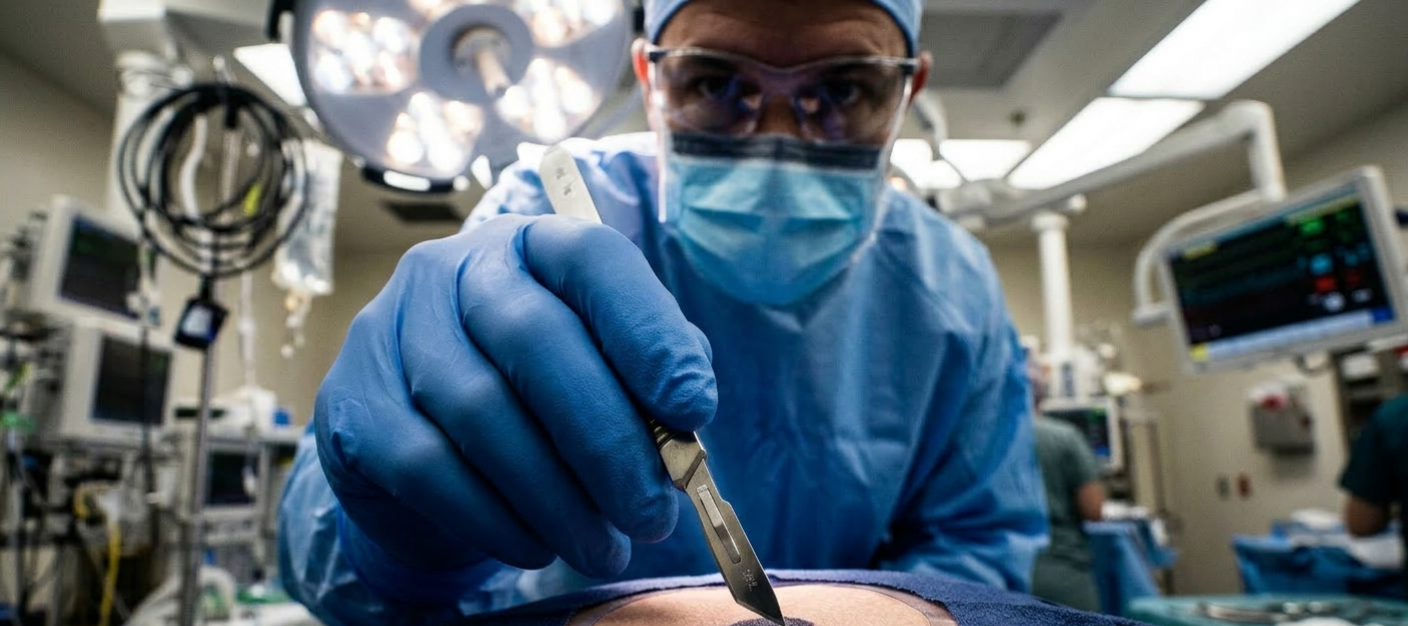
\includegraphics[keepaspectratio]{IMAGENES/cirugia.png}}

}

\caption{\label{fig-enfoques}Saber, saber hacer, saber ser (Imágen
creada con IA)}

\end{figure}%

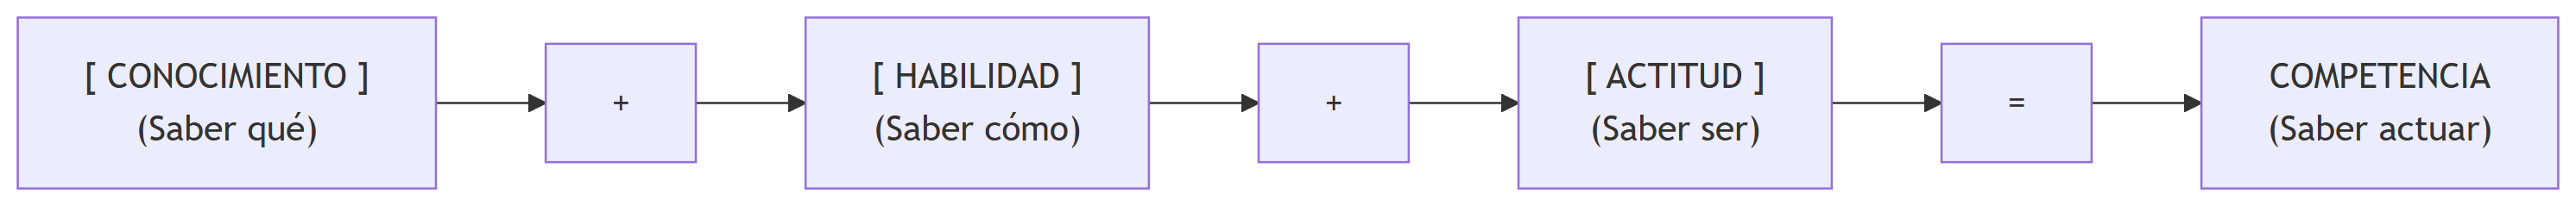
\includegraphics[width=12.22in,height=0.98in]{01_pautas_files/figure-latex/mermaid-figure-1.png}

Modelo de competencias en Bioestadística

\begin{tcolorbox}[enhanced jigsaw, arc=.35mm, bottomrule=.15mm, bottomtitle=1mm, breakable, colback=white, colbacktitle=quarto-callout-note-color!10!white, colframe=quarto-callout-note-color-frame, coltitle=black, left=2mm, leftrule=.75mm, opacityback=0, opacitybacktitle=0.6, rightrule=.15mm, title=\textcolor{quarto-callout-note-color}{\faInfo}\hspace{0.5em}{Descripción de la cursada}, titlerule=0mm, toprule=.15mm, toptitle=1mm]

\begin{itemize}
\item
  La modalidad del dictado presencial es de
  \texttt{tipo\ taller\ o\ laboratorio\ de\ análisis\ estadístico},
  donde los alumnos deben \texttt{aplicar} los conceptos desarrollados
  durante la introducción teórica en la resolución de ejercicios
  propuestos utilizando software estadístico. A tal fin, se admite la
  conformación de
  \texttt{grupos\ de\ hasta\ dos\ estudiantes\ por\ computadora}. Los
  estudiantes tendrán libertad de asistir a cualquiera de las comisiones
  prácticas, siempre y cuando hayan asistido previamente a la clase
  teórica del tema en curso, debido a que la cátedra adoptará una
  modalidad teórico-práctica.
\item
  Las actividades se complementan con al menos una actividad de campo,
  para la obtención de datos y su posterior análisis y aplicación de los
  métodos aprendidos.
\item
  También se implementa un trabajo o Proyecto de Investigación, en el
  cual los estudiantes deben analizar datos proporcionados en el
  contexto de casos reales o publicaciones realizadas y comparar sus
  conclusiones y el planteo de resolución que propusieron, con los
  descritos en las publicaciones. O bien, la aplicación de análisis de
  datos en estudios que hayan realizado previamente para otras materias.
\item
  Existe una instancia de evaluación permanente por medio de ejercicios
  de entrenamiento y auto-evaluación proporcionados en el Aula Virtual,
  que los alumnos deben resolver fuera del horario de clase. Estos
  ejercicios estarán acompañados por mecanismos de
  \texttt{retroalimentación} en la forma de encuestas y monitoreo para
  realizar el seguimiento de sus actividades.
  \texttt{Deberán\ tener\ aprobadas\ todas\ las\ actividades\ de\ entrenamiento\ para\ poder\ acceder\ a\ los\ parciales\ correspondientes}.
\item
  La nota obtenida en cada parcial se compone de un
  \texttt{promedio\ entre\ la\ nota\ del\ parcial\ y\ de\ las\ actividades\ prácticas}.
\end{itemize}

\end{tcolorbox}

\bookmarksetup{startatroot}

\chapter{Competencias prácticas de la
bioestadística}\label{competencias-pruxe1cticas-de-la-bioestaduxedstica}

\section{Niveles de competencias}\label{niveles-de-competencias}

Se adopta la jerarquía de niveles de conocimiento estadístico propuesta
por \textbf{Ben-Zvi y Garfield (2005)}: a) alfabetización estadística,
b) razonamiento estadístico y c) pensamiento estadístico, como un
continuo de desarrollo formativo, adaptado a un entorno de múltiples
herramientas informáticas. Desde una perspectiva práctica, esto
significa que cada nivel no solo se declara, sino que se pone en juego
en la resolución concreta de los ejercicios propuestos. El motivo es que
el profesional no sólo debe reconocer qué procedimiento estadístico es
adecuado para cada situación, sino que también debe saber cómo
implementarlo.

Cada nivel de conocimiento estadístico se construye sobre el anterior,
incorporando progresivamente elementos de niveles superiores a lo largo
de la cursada.

\begin{itemize}
\item
  Alfabetización estadística: representa la comprensión del ``qué''
  (conceptos, gráficos, símbolos, funciones). En la práctica, supone
  reconocer el procedimiento o sintaxis necesarios para ejecutar una
  prueba, leer correctamente su salida y verificar que no haya errores
  de especificación en el software elegido. Constituye la base en las
  competencias estadísticas.
\item
  Razonamiento estadístico: capacidad de seleccionar y justificar
  procedimientos, interpretar resultados más allá de la consigna y
  detectar errores. En la práctica, supone tareas como elegir la prueba
  estadística adecuada ante un problema dado, explicar por qué se
  rechaza o no una hipótesis, o detectar que un gráfico generado por
  software no es apropiado para los datos analizados.
\item
  Pensamiento estadístico: comprensión del ``para qué'' y ``en qué
  contexto'', formular problemas en términos estadísticos, reconocer la
  variabilidad como un aspecto inherente, evaluar supuestos, conectar
  datos con procesos generadores, tomar decisiones bajo incertidumbre,
  comunicar conclusiones con rigor disciplinar.
\end{itemize}

~

\begin{tcolorbox}[enhanced jigsaw, arc=.35mm, bottomrule=.15mm, bottomtitle=1mm, breakable, colback=white, colbacktitle=quarto-callout-note-color!10!white, colframe=quarto-callout-note-color-frame, coltitle=black, left=2mm, leftrule=.75mm, opacityback=0, opacitybacktitle=0.6, rightrule=.15mm, title=\textcolor{quarto-callout-note-color}{\faInfo}\hspace{0.5em}{Objetivo del curso (actividades prácticas)}, titlerule=0mm, toprule=.15mm, toptitle=1mm]

El objetivo mínimo de este curso es que, al finalizar, cada estudiante
demuestre al menos habilidades relacionadas con el \textbf{razonamiento
estadístico} en problemas estructurados, y principios de
\textbf{pensamiento estadístico} en problemas abiertos de su disciplina:
no se exige dominio pleno del pensamiento estadístico, pero sí que el
estudiante sea capaz de identificar cuándo el razonamiento no es
suficiente y qué preguntas de contexto quedan abiertas.

\end{tcolorbox}

En virtud de lo anterior, ciertos contenidos usualmente incluidos en
cursos introductorios de bioestadística (como algunos tipos de gráficos,
ciertas distribuciones de probabilidad, etc.) han sido deliberadamente
omitidos a fin de priorizar un tratamiento en mayor profundidad de
aquellos conceptos y herramientas que se considera permiten desarrollar
mejor los criterios de análisis, interpretación y toma de decisiones.

\begin{center}\rule{0.5\linewidth}{0.5pt}\end{center}

\section{Evaluación práctica}\label{evaluaciuxf3n-pruxe1ctica}

La propuesta didáctica de este material se inspira en recomendaciones
internacionales para la enseñanza de la estadística, como el estándar
\textbf{GAISE}, adaptándolas al contexto de formación situada en la
provincia de Jujuy.

\begin{tcolorbox}[enhanced jigsaw, arc=.35mm, bottomrule=.15mm, bottomtitle=1mm, breakable, colback=white, colbacktitle=quarto-callout-note-color!10!white, colframe=quarto-callout-note-color-frame, coltitle=black, left=2mm, leftrule=.75mm, opacityback=0, opacitybacktitle=0.6, rightrule=.15mm, title=\textcolor{quarto-callout-note-color}{\faInfo}\hspace{0.5em}{Metas del estándar GAISE}, titlerule=0mm, toprule=.15mm, toptitle=1mm]

\begin{enumerate}
\def\labelenumi{\arabic{enumi}.}
\tightlist
\item
  Enseñar pensamiento estadístico.
\item
  Enseñar la estadística como un proceso de investigación para la
  resolución de problemas y la toma de decisiones.
\item
  Brindar a los estudiantes experiencia en pensamiento multivariable.
\item
  Enfocarse en la comprensión conceptual.
\item
  Integrar datos reales con un contexto y un propósito.
\item
  Fomentar el aprendizaje activo.
\item
  Utilizar la tecnología para explorar conceptos y analizar datos.
\item
  Usar evaluaciones para mejorar y valorar el aprendizaje de los
  estudiantes.
\end{enumerate}

\end{tcolorbox}

Con ese marco, al finalizar el curso, \textbf{cada estudiante debe ser
capaz de}:

\begin{itemize}
\tightlist
\item
  \texttt{Seleccionar\ y\ aplicar\ correctamente}, de forma autónoma,
  una técnica estadística ante un problema concreto.
\item
  \texttt{Justificar\ su\ elección} (supuestos, limitaciones,
  alternativas).
\item
  \texttt{Ejecutar\ correctamente} la técnica estadística seleccionada
  en al menos un entorno de software (acción y resultado).
\item
  \texttt{Interpretar\ los\ resultados} tanto en términos estadísticos
  como disciplinares: agronomía, biología, ciencias ambientales,
  bromatología, etc.
\item
  Poder \texttt{identificar\ al\ menos\ una\ fuente\ de\ variabilidad}
  no controlada en el problema.
\item
  \texttt{Señalar\ una\ limitación\ del\ análisis} que requeriría datos
  adicionales, un ajuste del diseño o un análisis diferente.
\end{itemize}

\begin{center}\rule{0.5\linewidth}{0.5pt}\end{center}

\begin{tcolorbox}[enhanced jigsaw, arc=.35mm, bottomrule=.15mm, bottomtitle=1mm, breakable, colback=white, colbacktitle=quarto-callout-warning-color!10!white, colframe=quarto-callout-warning-color-frame, coltitle=black, left=2mm, leftrule=.75mm, opacityback=0, opacitybacktitle=0.6, rightrule=.15mm, title=\textcolor{quarto-callout-warning-color}{\faExclamationTriangle}\hspace{0.5em}{Modalidad de las evaluaciones}, titlerule=0mm, toprule=.15mm, toptitle=1mm]

\begin{itemize}
\item
  Los parciales serán presenciales y podrán ser realizados en grupos de
  hasta 2 (dos) personas. Deberán contar con una computadora ya que
  deberán realizar cálculos estadísticos (tomar las previsiones con
  tiempo, informar a la cátedra si se dificulta contar con una
  computadora para tratar de resolver la situación). En función de la
  cantidad de estudiantes, el formato de entrega podrá ser escrito o
  bien mediante la entrega del script con la resolución de los
  ejercicios. Además de la entrega, los parciales deberán ser
  defendidos/validados en forma oral, cuya implementación será
  oportunamente consensuada.
\item
  Los informes de análisis y tareas de campo deberán ser defendidas en
  forma oral, cuya implementación será oportunamente consensuada.
\end{itemize}

\end{tcolorbox}

\begin{center}\rule{0.5\linewidth}{0.5pt}\end{center}

\section{Estrategia pedagógica}\label{estrategia-pedaguxf3gica}

Se propone una integración gradual entre la práctica guiada y la
construcción del razonamiento. Desde la primera clase se combinan:

\begin{itemize}
\tightlist
\item
  \textbf{Secuencias simples de manipulación y análisis de datos} con
  software estadístico especializado, como mecanismos de
  estímulo-respuesta (acción - resultado inmediato) que permiten al
  alumno asociar rápidamente una operación, como hacer click en un menú
  o ejecutar una línea de código, obteniendo una salida numérica o
  gráfica, generando así un primer anclaje sobre conceptos abstractos.
\item
  \textbf{Ejercicios dirigidos} (para fijar alfabetización y primeros
  pasos del razonamiento).
\item
  \textbf{Preguntas de reflexión crítica} (¿por qué un gráfico puede
  sugerir comportamientos atípicos? ¿qué pasaría si se modifican valores
  en el set de datos?).
\item
  \textbf{Análisis y discusión de datos reales} (para desarrollar un
  sentido crítico y razonamiento estadístico).
\end{itemize}

\texttt{Las\ clases\ prácticas\ se\ organizarán\ en\ dos\ etapas:\ la\ primera\ etapa,\ hasta\ el\ primer\ parcial,\ tendrá\ una\ orientación\ principalmente\ focalizada\ en\ lograr\ que\ los\ estudiantes\ adquieran\ destrezas\ procedimentales\ de\ análisis\ estadístico,\ tanto\ en\ el\ manejo\ conceptual\ de\ terminología\ estadística\ orientada\ a\ su\ aplicación,\ como\ la\ manipulación\ del\ software\ estadístico.\ Es\ por\ ello\ que\ se\ aplicará\ una\ estrategia\ de\ aprendizaje\ basado\ en\ problemas\ (ejercicios).\ Una\ vez\ finalizada\ esta\ etapa,\ se\ asumirá\ que\ el\ estudiante\ ya\ cuenta\ con\ las\ competencias\ básicas\ para\ avanzar\ hacia\ el\ desarrollo\ del\ razonamiento\ y\ el\ pensamiento\ estadístico,\ momento\ en\ que\ se\ incorporará,\ además,\ un\ enfoque\ basado\ en\ proyectos}.

En este marco, se reconoce una progresión en los niveles de aprendizaje:

\begin{enumerate}
\def\labelenumi{\arabic{enumi}.}
\tightlist
\item
  Cuando el estudiante se centra en la sintaxis de un programa o en la
  identificación de procedimientos adecuados, se encuentra en una etapa
  de alfabetización estadística.
\item
  Cuando es capaz de justificar la elección de un método o modelo en
  función de los datos, avanza hacia el razonamiento estadístico.
\item
  Cuando cuestiona la adecuación de ese modelo considerando los
  mecanismos subyacentes del fenómeno en estudio, incorpora elementos
  del pensamiento estadístico.
\end{enumerate}

Esta secuencia no debe interpretarse como etapas rígidas o lineales,
sino como niveles que se superponen y retroalimentan a lo largo del
proceso de aprendizaje.

\begin{center}\rule{0.5\linewidth}{0.5pt}\end{center}

\section{Estrategias de estudio}\label{estrategias-de-estudio}

Las siguientes estrategias están orientadas a fortalecer el razonamiento
estadístico y mejorar la comunicación de resultados, priorizando la
comprensión de los conceptos por sobre la aplicación mecánica de
técnicas. Su objetivo es guiar el estudio y la preparación de
evaluaciones, promoviendo una mirada integrada entre teoría, práctica e
interpretación.

\begin{itemize}
\tightlist
\item
  Comprender antes de memorizar: identificar qué problema estadístico
  resuelve cada método.
\item
  Practicar interpretación: explicar siempre qué significa un resultado
  en términos de un fenómeno real.
\item
  Conectar conceptos: vincular muestreo, inferencia, modelos y diseño
  experimental.
\item
  Preparar ejemplos: practicar la explicación con una o dos situaciones
  de ejemplo. Aplicar el lema: \emph{``ejemplos, ejemplos y más
  ejemplos''}.
\item
  Explicar supuestos: todo método estadístico tiene condiciones de
  validez.
\item
  Pensar como investigador: preguntarse siempre cuál es la pregunta
  científica.
\item
  Sostener el razonamiento: si no se recuerda una fórmula exacta,
  explicar el razonamiento estadístico.
\end{itemize}

~

\begin{tcolorbox}[enhanced jigsaw, arc=.35mm, bottomrule=.15mm, bottomtitle=1mm, breakable, colback=white, colbacktitle=quarto-callout-tip-color!10!white, colframe=quarto-callout-tip-color-frame, coltitle=black, left=2mm, leftrule=.75mm, opacityback=0, opacitybacktitle=0.6, rightrule=.15mm, title=\textcolor{quarto-callout-tip-color}{\faLightbulb}\hspace{0.5em}{Jerarquía para explicar un problema estadístico}, titlerule=0mm, toprule=.15mm, toptitle=1mm]

Es importante poder explicar cualquier problema estadístico en el
siguiente orden jerárquico:

\begin{enumerate}
\def\labelenumi{\arabic{enumi}.}
\tightlist
\item
  \textbf{Pregunta de investigación} (o problema a resolver)
\item
  \textbf{Datos} (reconocer variables, estructura, procedencia, calidad,
  etc.)
\item
  \textbf{Descripción} (caracterizar estadísticamente los datos)
\item
  \textbf{Método a utilizar} (incluye especificar criterios de selección
  del método o modelo)
\item
  \textbf{Resultado}
\item
  \textbf{Interpretación}
\item
  \textbf{Comunicación}
\end{enumerate}

\end{tcolorbox}

\begin{center}\rule{0.5\linewidth}{0.5pt}\end{center}

\section{Inteligencia artificial generativa: Pautas de trabajo en el
curso}\label{inteligencia-artificial-generativa-pautas-de-trabajo-en-el-curso}

En 2024, la UNESCO (2024) publicó la \emph{Guía para el uso de IA
generativa en educación e investigación}. En ella, recomienda:

\begin{tcolorbox}[enhanced jigsaw, arc=.35mm, bottomrule=.15mm, bottomtitle=1mm, breakable, colback=white, colbacktitle=quarto-callout-note-color!10!white, colframe=quarto-callout-note-color-frame, coltitle=black, left=2mm, leftrule=.75mm, opacityback=0, opacitybacktitle=0.6, rightrule=.15mm, title=\textcolor{quarto-callout-note-color}{\faInfo}\hspace{0.5em}{Recomendación UNESCO (2024)}, titlerule=0mm, toprule=.15mm, toptitle=1mm]

\begin{quote}
\emph{``Evitar el uso de la IA generativa cuando pudiera privar a los
estudiantes de oportunidades para desarrollar capacidades cognitivas a
través del razonamiento lógico independiente.''}
\end{quote}

\end{tcolorbox}

Esta recomendación guiará el enfoque pedagógico adoptado en el presente
curso, orientando el uso de estas herramientas hacia un rol
complementario y no sustitutivo del aprendizaje.

El desarrollo vertiginoso de la inteligencia artificial generativa
(IAGEN o simplemente IA) supone la coexistencia de dos aspectos
complementarios, inseparables, con implicancias profundas en el proceso
de formación profesional:

\begin{enumerate}
\def\labelenumi{\arabic{enumi}.}
\tightlist
\item
  \textbf{Oportunidad extraordinaria}: permite lograr una formación
  técnica y profesional de mayor profundidad, superando limitaciones de
  accesibilidad a la información y aspectos técnicos u operativos para
  focalizar en las bases científicas y éticas del conocimiento.
\item
  \textbf{Responsabilidad y desafío}: exige desarrollar un uso crítico,
  reflexivo y éticamente fundamentado, evitando la delegación acrítica
  del razonamiento. Se vuelve central fortalecer la capacidad de
  formular problemas, evaluar la pertinencia de métodos, validar
  resultados y sostener una interpretación fundada en criterios
  disciplinares.
\end{enumerate}

\subsection{¿Qué puede aportar la IA en
Bioestadística?}\label{quuxe9-puede-aportar-la-ia-en-bioestaduxedstica}

\begin{itemize}
\tightlist
\item
  Explicar qué hace una función, o interpretar un mensaje de error.
\item
  Sugerir código o secuencias de análisis para resolver tareas
  analíticas.
\item
  Reformular explicaciones estadísticas desde distintos enfoques.
\item
  Proponer alternativas cuando un procedimiento no funciona.
\end{itemize}

\subsection{Lo que la IA NO puede
hacer}\label{lo-que-la-ia-no-puede-hacer}

\begin{itemize}
\tightlist
\item
  \textbf{Comprender} el contexto específico del análisis, ni asumir las
  consecuencias de los resultados obtenidos.
\item
  \textbf{Garantizar} que el código generado o la secuencia de análisis
  propuesta sean correctos para un determinado problema.
\item
  \textbf{Sustituir el criterio} para elegir una medida o un método
  estadístico.
\item
  \textbf{Interpretar resultados} con fundamento disciplinar
  (agronómico, bromatológico, biológico o ambiental).
\end{itemize}

\subsection{Esquema de trabajo
propuesto}\label{esquema-de-trabajo-propuesto}

Se propone el siguiente esquema de trabajo con herramientas de IA (como
\textbf{NotebookLM} de Google u opciones similares):

\begin{enumerate}
\def\labelenumi{\arabic{enumi}.}
\tightlist
\item
  \textbf{Crear un espacio de trabajo} (carpeta o notebook) y llamarlo
  con el nombre de la materia: \texttt{Bioestadística}.
\item
  \textbf{Cargar los materiales del curso}:

  \begin{itemize}
  \tightlist
  \item
    La guía: \emph{Apuntes de Bioestadística con ejercicios resueltos}.
  \item
    La bibliografía sugerida por la cátedra.
  \end{itemize}
\item
  \textbf{Interactuar bajo el rol de asistente pedagógico}:

  \begin{itemize}
  \tightlist
  \item
    Resolver dudas conceptuales.
  \item
    Guiar el aprendizaje mediante preguntas orientadoras.
  \item
    Generar explicaciones alternativas (analogías, ejemplos).
  \item
    Producir recursos complementarios (cuestionarios, esquemas,
    resúmenes, etc.).
  \item
    Entender mensajes de error.
  \item
    Comprender la sintaxis u opciones en diferentes programas
    estadísticos.
  \item
    Explorar alternativas de análisis.
  \end{itemize}
\end{enumerate}

~

\begin{tcolorbox}[enhanced jigsaw, arc=.35mm, bottomrule=.15mm, bottomtitle=1mm, breakable, colback=white, colbacktitle=quarto-callout-warning-color!10!white, colframe=quarto-callout-warning-color-frame, coltitle=black, left=2mm, leftrule=.75mm, opacityback=0, opacitybacktitle=0.6, rightrule=.15mm, title=\textcolor{quarto-callout-warning-color}{\faExclamationTriangle}\hspace{0.5em}{Criterios de precaución y verificación obligatoria}, titlerule=0mm, toprule=.15mm, toptitle=1mm]

\begin{itemize}
\tightlist
\item
  Naturaleza Probabilística: Las herramientas de IA operan mediante
  modelos probabilísticos de lenguaje y no mediante algoritmos lógicos o
  fórmulas matemáticas cerradas. Por lo tanto, pueden generar
  ``alucinaciones'', produciendo explicaciones que parecen técnicamente
  coherentes, pero que no siempre son coherentes con los fundamentos
  teóricos de la estadística.
\item
  Prevalencia bibliográfica: En caso de discrepancia entre una
  explicación generada por la IA y los marcos conceptuales desarrollados
  en la bibliografía propuesta por la cátedra, \textbf{deben prevalecer
  siempre el contenido de la obra y la bibliografía académica}.
\item
  Criterio disciplinar: El criterio del investigador es el único capaz
  de validar si una interpretación es agronómica, biológica, ambiental o
  bromatológicamente plausible, más allá de la corrección sintáctica del
  código sugerido.
\item
  Verificación Obligatoria: Todo código generado (especialmente en R,
  Python o Julia) debe ser verificado. Pequeños errores en funciones
  (por ejemplo, confundir parámetros de varianza con desvío estándar)
  pueden invalidar completamente una prueba.
\end{itemize}

\end{tcolorbox}

\bookmarksetup{startatroot}

\chapter{Trabajo Práctico 0: Introducción al manejo de
R}\label{trabajo-pruxe1ctico-0-introducciuxf3n-al-manejo-de-r}

\section{Primeros pasos}\label{primeros-pasos}

\begin{itemize}
\tightlist
\item
  La instalación del lenguaje \textbf{R} puede realizarse desde la
  \textbf{Red Integral de Archivos de R (CRAN)}. En esta interface se
  debe seleccionar el sistema operativo que corresponda, por ejemplo
  \textbf{WINDOWS}. En la siguiente interface, seleccionar \textbf{base}
  (o bien \textbf{``install R for the first time''}) y, finalmente, en
  la siguiente pantalla, seleccionar Download R-4.4.2 for Windows (o la
  versión que se desee). Se descargará un archivo ejecutable con el
  instalador del lenguaje, el cual deberemos correr aceptando todas las
  instancias.
\end{itemize}

~

~

\begin{itemize}
\tightlist
\item
  \textbf{RStudio} es un \emph{entorno de desarrollo integrado}
  (\textbf{IDE}, por sus siglas en inglés) para el lenguaje de
  programación R, que ofrece una interfaz gráfica de usuario (GUI)
  amigable y diversas herramientas para facilitar el desarrollo,
  depuración y visualización de código. Entre sus características se
  incluyen la edición de código con resaltado de sintaxis, la ejecución
  de código línea por línea o por bloques, la gestión de paquetes, la
  creación de gráficos y la integración con otros programas y
  herramientas para el análisis de datos.
\end{itemize}

~

\begin{center}
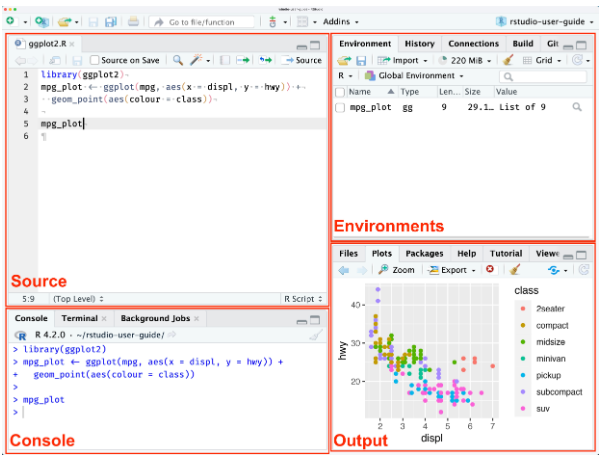
\includegraphics[width=1\linewidth,height=\textheight,keepaspectratio]{1.png}
\end{center}

\begin{itemize}
\tightlist
\item
  \textbf{RStudioCloud}: Actualmente administrada por la compañía
  \emph{Posit}, permite trabajar con Rstudio en la nube. Es necesario
  crear un cuenta (``Sign up'') cuando se accede por primera vez, o bien
  ingresar los datos de acceso (``log in'') en caso de que ya se posea
  una cuenta. La versión gratuita permite actualmente trabajar hasta con
  50 proyectos y 25 horas de trabajo mensuales.
\end{itemize}

\textbf{\emph{Enlaces}}

\begin{itemize}
\item
  \href{https://cran.r-project.org/}{CRAN(``click'')}. Descarga del
  \textbf{\emph{lenguaje}} R.
\item
  \href{https://www.rstudio.com/products/rstudio/download/}{Rstudio(``click'')}.
  Descarga del \textbf{\emph{IDE}} RStudio.
\item
  \href{https://posit.cloud/plans/free}{Rstudio Cloud(``click'')}.
\end{itemize}

\begin{tcolorbox}[enhanced jigsaw, arc=.35mm, bottomrule=.15mm, bottomtitle=1mm, breakable, colback=white, colbacktitle=quarto-callout-note-color!10!white, colframe=quarto-callout-note-color-frame, coltitle=black, left=2mm, leftrule=.75mm, opacityback=0, opacitybacktitle=0.6, rightrule=.15mm, title=\textcolor{quarto-callout-note-color}{\faInfo}\hspace{0.5em}{Compatibilidad}, titlerule=0mm, toprule=.15mm, toptitle=1mm]

R 4.1 es la última versión compatible con versiones de 32 bits. Windows
Vista ya no es compatible.

R 4.2.0 y versiones posteriores requieren Universal C Runtime (UCRT),
que se incluye en Windows 10 y Windows Server 2016 o posterior. En
versiones anteriores de Windows, UCRT debe instalarse antes de instalar
R. UCRT está disponible para Windows desde Windows Vista SP2 y Windows
Server 2008 SP2.

\end{tcolorbox}

\begin{tcolorbox}[enhanced jigsaw, arc=.35mm, bottomrule=.15mm, bottomtitle=1mm, breakable, colback=white, colbacktitle=quarto-callout-tip-color!10!white, colframe=quarto-callout-tip-color-frame, coltitle=black, left=2mm, leftrule=.75mm, opacityback=0, opacitybacktitle=0.6, rightrule=.15mm, title=\textcolor{quarto-callout-tip-color}{\faLightbulb}\hspace{0.5em}{Importante}, titlerule=0mm, toprule=.15mm, toptitle=1mm]

Antes de instalar \emph{RStudio}, tienes que haber instalado R.

\end{tcolorbox}

\subsection{Otros IDE}\label{otros-ide}

\begin{itemize}
\item
  \href{https://www.navure.com/inicio/}{Navure (``click'')}
\item
  \href{https://www.infostat.com.ar/}{InfoStat (``click'')}
\item
  \href{https://jupyter.org/}{Jupyter (``click'')}
\item
  \href{https://jasp-stats.org/download/}{JASP (``click'')}
\item
  \href{https://www.jamovi.org/download.html}{JAMOVI (``click'')}
\item
  \href{https://projects.eclipse.org/projects/science.statet}{StatET
  (``click'')}
\item
  \href{https://ess.r-project.org/}{ESS (``click'')}
\item
  \href{http://r.analyticflow.com/en/}{R Analytic flow (``click'')}
\item
  \href{https://rattle.togaware.com/}{Rattle (``click'')}
\end{itemize}

\begin{tcolorbox}[enhanced jigsaw, arc=.35mm, bottomrule=.15mm, bottomtitle=1mm, breakable, colback=white, colbacktitle=quarto-callout-tip-color!10!white, colframe=quarto-callout-tip-color-frame, coltitle=black, left=2mm, leftrule=.75mm, opacityback=0, opacitybacktitle=0.6, rightrule=.15mm, title=\textcolor{quarto-callout-tip-color}{\faLightbulb}\hspace{0.5em}{Tip}, titlerule=0mm, toprule=.15mm, toptitle=1mm]

\textbf{¡¡¡ R PUEDE SER EJECUTADO SIN NECESIDAD DE UN IDE!!!}

Por ejemplo, en la barra de búsqueda de \emph{Windows}, seleccionar
\textbf{Editar las variables de entorno de esta cuenta}. Aparecerá la
ventana \textbf{Variables de entorno}. En el bloque \textbf{Variables de
usuario para usuario}, seleccionar \textbf{Path} y luego presionar
\textbf{Editar\ldots{}}. Aparecerá la ventana \textbf{Editar las
variables de entorno}. Presionar la opción \textbf{Nuevo} e ingresar
\textbf{C:\textbackslash Program
Files\textbackslash R\textbackslash R-4.4.2\textbackslash bin} (o la
versión que se desee). Finalmente, \emph{Aceptar}.

Desde ahora podremos correr código R desde la ventana de comandos
\textbf{Símbolo del sistema}, a la cual se accede ingresando el comando
\textbf{CMD} en la barra de búsqueda de \emph{Windows}. Basta ejecutar
el comando \textbf{r} para comenzar a correr código de R, y \textbf{q()}
para salir.

\end{tcolorbox}

\section{Objetos}\label{objetos}

``Todo en R es un objeto''

Se conoce como objeto a toda entidad creada y manipulada en \textbf{R}.
Datos, tablas, gráficos, funciones, vectores, matrices, son algunos
tipos de objetos en R.

Los objetos en R se caracterizan porque pueden presentar distintos
atributos, por ejemplo, un nombre. Esto quiere decir que al momento de
almacenar un objeto es posible asignarle un nombre.

\begin{tcolorbox}[enhanced jigsaw, arc=.35mm, bottomrule=.15mm, bottomtitle=1mm, breakable, colback=white, colbacktitle=quarto-callout-note-color!10!white, colframe=quarto-callout-note-color-frame, coltitle=black, left=2mm, leftrule=.75mm, opacityback=0, opacitybacktitle=0.6, rightrule=.15mm, title=\textcolor{quarto-callout-note-color}{\faInfo}\hspace{0.5em}{\textbf{Nota}}, titlerule=0mm, toprule=.15mm, toptitle=1mm]

Al momento de nombrar un objeto en \textbf{R}, es importante utilizar
nombres claros y cortos que permitan manipular con sencillez el objeto.
También se sugiere utilizar nombres que permitan recordar fácilmente el
contenido de los objetos.

Los nombres pueden incluir letras, números (siempre y cuando estén
precedidos por una letra), guión bajo y puntos (antes o después de las
letras). No se pueden utilizar símbolos especiales (``*'', ``:'', ``-'',
``\textasciitilde{}'',``\$'', entre otros) ni palabras reservadas (NA,
for, while, TRUE, FALSE, Inf, NaN, NULL) en la denominación de un
objeto.

\textbf{R} distingue mayúsculas y minúsculas, por lo que las variables
\emph{a} y \emph{A} serán consideradas como objetos diferentes.

\end{tcolorbox}

Podemos almacenar los datos en variables por medio del operador ``='' o
bien por medio de los operadores de asignación ``\textless-'' o
``-\textgreater{}''. También podemos asignar valores utilizando la
función \textbf{assign()}.

La función \textbf{class()} nos devuelve el atributo \emph{tipo de
dato}.

\begin{Shaded}
\begin{Highlighting}[]
\NormalTok{a }\OtherTok{=} \DecValTok{1}
\NormalTok{a}
\FunctionTok{class}\NormalTok{(a)}

\NormalTok{a }\OtherTok{\textless{}{-}} \DecValTok{1}
\NormalTok{a}
\FunctionTok{class}\NormalTok{(a)}

\DecValTok{1} \OtherTok{{-}\textgreater{}}\NormalTok{ a}
\NormalTok{a}
\FunctionTok{class}\NormalTok{(a)}

\FunctionTok{assign}\NormalTok{(}\StringTok{"a"}\NormalTok{, }\DecValTok{1}\NormalTok{)}
\NormalTok{a}
\FunctionTok{class}\NormalTok{(a)}
\end{Highlighting}
\end{Shaded}

\begin{tcolorbox}[enhanced jigsaw, arc=.35mm, bottomrule=.15mm, bottomtitle=1mm, breakable, colback=white, colbacktitle=quarto-callout-note-color!10!white, colframe=quarto-callout-note-color-frame, coltitle=black, left=2mm, leftrule=.75mm, opacityback=0, opacitybacktitle=0.6, rightrule=.15mm, title=\textcolor{quarto-callout-note-color}{\faInfo}\hspace{0.5em}{Nota}, titlerule=0mm, toprule=.15mm, toptitle=1mm]

Notar que las asignaciones se realizaron de derecha a izquierda en los
dos primeros casos, y de izquierda a derecha en el tercero. La práctica
más extendida es realizar la asignación de derecha a izquierda.

\end{tcolorbox}

\emph{Ejemplos de atributos}

\begin{itemize}
\item
  Class
\item
  Dim: dimensión (matrices, dataframes, arreglos)
\item
  Names: nombre de los componentes de un objeto
\item
  Length: longitud de un vector.
\item
  Ncol, Nrow: número de columnas/filas (en matrices, dataframes, etc.)
\item
  Frecuency: frecuencia en una serie de tiempo
\item
  Etc.
\end{itemize}

\begin{tcolorbox}[enhanced jigsaw, arc=.35mm, bottomrule=.15mm, bottomtitle=1mm, breakable, colback=white, colbacktitle=quarto-callout-note-color!10!white, colframe=quarto-callout-note-color-frame, coltitle=black, left=2mm, leftrule=.75mm, opacityback=0, opacitybacktitle=0.6, rightrule=.15mm, title=\textcolor{quarto-callout-note-color}{\faInfo}\hspace{0.5em}{Tipos de datos}, titlerule=0mm, toprule=.15mm, toptitle=1mm]

En R, los tipos de datos principales se pueden agrupar en \textbf{tipos
atómicos}, que son las unidades mínimas de información, y las
\textbf{estructuras de datos}. Los principales tipos de datos atómicos
son:

\begin{itemize}
\item
  numeric: son datos numéricos. Un caso especial de datos numéricos es
  el tipo integer (entero).
\item
  character: son datos de tipo texto
\item
  logical: son datos lógicos, que pueden adoptar uno de dos valores:
  TRUE o FALSE.
\item
  complex: Números complejos, por ejemplo a = 2 + 3i.
\end{itemize}

También puede mencionarse el tipo de dato raw, usado para almacenar
secuencias de bytes útiles para trabajar con datos binarios, pero su
empleo se realiza en contextos muy específicos, por lo que usualmente no
trabajaremos con ellos.

Además, según la estructura de los datos, los objetos pueden ser:

\begin{itemize}
\item
  Vectores: son series de objetos del mismo tipo atómico.
\item
  Matrices: son arreglos en filas y columnas de objetos del mismo tipo
  atómico.
\item
  Arreglos (``arrays''): extienden las matrices a más dimensiones.
\item
  Tablas(data.frames o tibbles): son arreglos en filas y columnas de
  objetos que pueden pertenecer a diferentes tipos atómicos.
\item
  Listas: son series de objetos que pueden presentar diferentes
  estructuras.
\item
  Factores: son series de objetos indexados o que presentan un
  ordenamiento jerárquico. Para indicar el índice de un objeto, se
  emplea {[}{[}{]}{]} en lugar de {[}{]}.
\end{itemize}

\end{tcolorbox}

\subsubsection{Ejemplos de clases de
datos}\label{ejemplos-de-clases-de-datos}

\begin{Shaded}
\begin{Highlighting}[]

\NormalTok{x }\OtherTok{=} \DecValTok{5}
\FunctionTok{class}\NormalTok{(x)}
\FunctionTok{mode}\NormalTok{(x)}

\NormalTok{x }\OtherTok{=} \DecValTok{5}\NormalTok{L}
\FunctionTok{class}\NormalTok{(x)}

\NormalTok{z }\OtherTok{=} \FunctionTok{seq}\NormalTok{(}\DecValTok{0}\NormalTok{, }\DecValTok{10}\NormalTok{, }\DecValTok{2}\NormalTok{) }\CommentTok{\# Secuencia: \textquotesingle{}desde\textquotesingle{}, \textquotesingle{}hasta\textquotesingle{}, \textquotesingle{}cada\textquotesingle{}}
\FunctionTok{class}\NormalTok{(z)}

\NormalTok{z }\OtherTok{=} \FunctionTok{as.integer}\NormalTok{(z)}
\FunctionTok{class}\NormalTok{(z)}

\NormalTok{sexo }\OtherTok{=} \FunctionTok{c}\NormalTok{(}\StringTok{"masculino"}\NormalTok{, }\StringTok{"femenino"}\NormalTok{)}
\FunctionTok{class}\NormalTok{(sexo)}

\NormalTok{notas }\OtherTok{=} \FunctionTok{c}\NormalTok{(}\StringTok{"1"}\NormalTok{, }\StringTok{"2"}\NormalTok{, }\StringTok{"3"}\NormalTok{, }\StringTok{"4"}\NormalTok{, }\StringTok{"5"}\NormalTok{, }\StringTok{"6"}\NormalTok{, }\StringTok{"7"}\NormalTok{, }\StringTok{"8"}\NormalTok{, }\StringTok{"9"}\NormalTok{, }\StringTok{"10"}\NormalTok{)}
\FunctionTok{class}\NormalTok{(notas)}
\FunctionTok{mean}\NormalTok{(notas)}
\NormalTok{notas }\OtherTok{=} \FunctionTok{as.numeric}\NormalTok{(notas)}
\FunctionTok{class}\NormalTok{(notas)}
\FunctionTok{mean}\NormalTok{(notas)}

\NormalTok{condicion }\OtherTok{=}\NormalTok{ (z }\SpecialCharTok{\textgreater{}}\NormalTok{ x)}
\NormalTok{condicion}
\FunctionTok{class}\NormalTok{(condicion)}

\NormalTok{complejo }\OtherTok{=} \DecValTok{2} \SpecialCharTok{+} \DecValTok{3}\NormalTok{i}
\NormalTok{complejo}
\FunctionTok{class}\NormalTok{(complejo)}

\NormalTok{calificacion }\OtherTok{=} \FunctionTok{factor}\NormalTok{(}\AttributeTok{levels =} \FunctionTok{c}\NormalTok{(}\StringTok{"insuficiente"}\NormalTok{,}\StringTok{"regular"}\NormalTok{,}\StringTok{"sobresaliente"}\NormalTok{))}
\NormalTok{calificacion}
\FunctionTok{class}\NormalTok{(calificacion)}

\NormalTok{factor.sexo }\OtherTok{=} \FunctionTok{as.factor}\NormalTok{(sexo)}
\NormalTok{factor.sexo}
\FunctionTok{class}\NormalTok{(factor.sexo)}

\NormalTok{matrizNotas }\OtherTok{=} \FunctionTok{matrix}\NormalTok{(notas, }\AttributeTok{nrow =} \DecValTok{5}\NormalTok{, }\AttributeTok{ncol =} \DecValTok{2}\NormalTok{)}
\NormalTok{matrizNotas}
\FunctionTok{class}\NormalTok{(matrizNotas)}

\NormalTok{serie }\OtherTok{=} \FunctionTok{seq}\NormalTok{(}\DecValTok{12}\NormalTok{)}
\NormalTok{serie}
\NormalTok{miArreglo }\OtherTok{=} \FunctionTok{array}\NormalTok{(serie, }\AttributeTok{dim =} \FunctionTok{c}\NormalTok{(}\DecValTok{2}\NormalTok{,}\DecValTok{2}\NormalTok{,}\DecValTok{2}\NormalTok{)) }\CommentTok{\# Las dimensiones hacen referencia al número de filas, número de columnas y número de capas, en ese orden}
\NormalTok{miArreglo}

\NormalTok{miLista }\OtherTok{=} \FunctionTok{list}\NormalTok{(sexo, notas, calificacion)}
\NormalTok{miLista}

\NormalTok{miLista1 }\OtherTok{=}\NormalTok{ miLista[[}\DecValTok{1}\NormalTok{]]}
\NormalTok{miLista1}
\FunctionTok{class}\NormalTok{(miLista1)}

\NormalTok{tabla }\OtherTok{=} \FunctionTok{data.frame}\NormalTok{(}
  \AttributeTok{Alumno =} \FunctionTok{c}\NormalTok{(}\StringTok{"Juan"}\NormalTok{, }\StringTok{"Ana"}\NormalTok{, }\StringTok{"María"}\NormalTok{), }\CommentTok{\# Columna 1}
  \AttributeTok{Notas =} \FunctionTok{c}\NormalTok{(}\DecValTok{5}\NormalTok{, }\DecValTok{8}\NormalTok{, }\DecValTok{10}\NormalTok{) }\CommentTok{\# Columna 2}
\NormalTok{)}
\NormalTok{tabla}
\end{Highlighting}
\end{Shaded}

\begin{tcolorbox}[enhanced jigsaw, arc=.35mm, bottomrule=.15mm, bottomtitle=1mm, breakable, colback=white, colbacktitle=quarto-callout-tip-color!10!white, colframe=quarto-callout-tip-color-frame, coltitle=black, left=2mm, leftrule=.75mm, opacityback=0, opacitybacktitle=0.6, rightrule=.15mm, title=\textcolor{quarto-callout-tip-color}{\faLightbulb}\hspace{0.5em}{Comentarios (\#)}, titlerule=0mm, toprule=.15mm, toptitle=1mm]

En \textbf{R}, toda línea precedida por el símbolo \# (numeral) no es
ejecutada. Su empleo es muy útil para realizar comentarios o
descripciones dentro del código.

\end{tcolorbox}

Los tipos de estructuras más utilizados en el análisis de datos
estadísticos son los vectores, matrices, tablas y factores.

Podemos ver que es posible modificar la tipología de un dato por otra,
de ser necesario. Algunas funciones utilizadas son:

\begin{itemize}
\item
  as.numeric(); as.integer()
\item
  as.character()
\item
  as.factor()
\item
  as.logical()
\item
  as.data.frame()
\item
  as.array()
\end{itemize}

\subsubsection{Borrado de objetos}\label{borrado-de-objetos}

Para borrar objetos almacenados, se utiliza la función \textbf{rm()}.

\begin{Shaded}
\begin{Highlighting}[]

\CommentTok{\# Borrado de un objeto}

\FunctionTok{rm}\NormalTok{(a)}
\NormalTok{a}
\CommentTok{\# Error: objeto \textquotesingle{}a\textquotesingle{} no encontrado}

\CommentTok{\# Borrado de todos los objetos en el entorno}

\FunctionTok{rm}\NormalTok{(}\AttributeTok{list =} \FunctionTok{ls}\NormalTok{())}
\end{Highlighting}
\end{Shaded}

\begin{tcolorbox}[enhanced jigsaw, arc=.35mm, bottomrule=.15mm, bottomtitle=1mm, breakable, colback=white, colbacktitle=quarto-callout-tip-color!10!white, colframe=quarto-callout-tip-color-frame, coltitle=black, left=2mm, leftrule=.75mm, opacityback=0, opacitybacktitle=0.6, rightrule=.15mm, title=\textcolor{quarto-callout-tip-color}{\faLightbulb}\hspace{0.5em}{Tip}, titlerule=0mm, toprule=.15mm, toptitle=1mm]

\textbf{Antes de comenzar cualquier análisis estadístico, se sugiere
borrar todos los objetos que pudieran estar almacenados en el entorno.}

\end{tcolorbox}

\begin{center}\rule{0.5\linewidth}{0.5pt}\end{center}

\section{Funciones}\label{funciones}

Todo lo que ocurre en R es el resultado de una función

Una función en \textbf{R} es un bloque de código que realiza una tarea
específica. Se la invoca por medio de un nombre seguido de paréntesis
que pueden contener argumentos si son necesarios. Por ejemplo:

\begin{Shaded}
\begin{Highlighting}[]

\NormalTok{a }\OtherTok{=} \DecValTok{30}

\NormalTok{b }\OtherTok{=} \DecValTok{20}

\FunctionTok{sort}\NormalTok{(}\FunctionTok{c}\NormalTok{(a, b))}

\FunctionTok{sum}\NormalTok{(a, b) }\CommentTok{\# equivalente a \textquotesingle{}a + b\textquotesingle{}}
\end{Highlighting}
\end{Shaded}

R tiene muchas funciones integradas para realizar diversas operaciones,
como cálculos matemáticos, manipulación de datos, gráficos, etc.
Ejemplos incluyen \textbf{sum()}, \textbf{mean()}, \textbf{length()},
\textbf{plot()}, \textbf{sort()}, entre otros. Aún así, es posible crear
funciones propias, lo cual se trabajará más adelante en la cursada.

\begin{center}\rule{0.5\linewidth}{0.5pt}\end{center}

\subsection{Paquetes}\label{paquetes}

En R, todas las funciones y sets de datos están almacenados en
\emph{paquetes}. Sólo cuando se \emph{cargue} un paquete su contenido
estará disponible. Ésto se realiza por una cuestión de eficiencia en el
uso de los recursos computacionales, y también por seguridad.

Algunos paquetes o \emph{librerías} forman parte del código fuente de R,
y son conocidos como librerías de \emph{base}, disponibles con la
instalación de R. El resto de las librerías deben ser instaladas desde
el \emph{CRAN}, mediante el comando \emph{install.packages(``nombre del
paquete'')}. En este último caso, para poder utilizar las funciones de
estas librerías, se debe correr el comando \emph{library(``nombre del
paquete'')}.

\begin{tcolorbox}[enhanced jigsaw, arc=.35mm, bottomrule=.15mm, bottomtitle=1mm, breakable, colback=white, colbacktitle=quarto-callout-note-color!10!white, colframe=quarto-callout-note-color-frame, coltitle=black, left=2mm, leftrule=.75mm, opacityback=0, opacitybacktitle=0.6, rightrule=.15mm, title=\textcolor{quarto-callout-note-color}{\faInfo}\hspace{0.5em}{Nota}, titlerule=0mm, toprule=.15mm, toptitle=1mm]

También es posible instalar paquetes desde un archivo previamente
descargado desde el CRAN. Para ello se puede correr el comando:

\textbf{install.packages(file.choose(), repos = NULL, type=``source'')}

\end{tcolorbox}

Por ejemplo, para importar archivos de datos con distintas extensiones,
se puede utilizar la función \textbf{import()} de la librería
\emph{\{rio\}}.

\begin{Shaded}
\begin{Highlighting}[]
\FunctionTok{install.packages}\NormalTok{(}\StringTok{"rio"}\NormalTok{) }\CommentTok{\# instalación de la librería (solo una vez)}
\FunctionTok{library}\NormalTok{(}\StringTok{"rio"}\NormalTok{) }\CommentTok{\# invocación de la librería (cada vez que deseemos utilizar alguna de sus funciones)}
\FunctionTok{import}\NormalTok{(}\FunctionTok{file.choose}\NormalTok{()) }\CommentTok{\# función import para leer archivos de datos y file.choose() para seleccionar archivos almacenados}
\end{Highlighting}
\end{Shaded}

Algunas de las librerías más utilizadas en R están ``empaquetadas'' en
la librería \emph{Tidyverse}.

\subsection{\texorpdfstring{Concatenación de funciones: el operador
``\textbar\textgreater{}''
(\emph{pipe})}{Concatenación de funciones: el operador ``\textbar\textgreater'' (pipe)}}\label{concatenaciuxf3n-de-funciones-el-operador-pipe}

Con frecuencia es necesario ``anidar'' funciones en \textbf{R}, por
ejemplo:

\begin{Shaded}
\begin{Highlighting}[]

\NormalTok{numeros }\OtherTok{=} \FunctionTok{seq}\NormalTok{(}\DecValTok{20}\NormalTok{)}
\NormalTok{numeros}
\FunctionTok{round}\NormalTok{(}\FunctionTok{sqrt}\NormalTok{(}\FunctionTok{mean}\NormalTok{(numeros)), }\AttributeTok{digits =} \DecValTok{2}\NormalTok{)}
\end{Highlighting}
\end{Shaded}

En la función anterior, la función \textbf{mean()} está anidada dentro
de la función \textbf{sqrt()}, que a su vez está anidada dentro de la
función \textbf{round()}. En estos casos, se dificulta llevar un control
de las operaciones realizadas, por lo que se suele recurrir al operador
\textbar\textgreater{} (``pipe''), que permite concatenar funciones:

\begin{Shaded}
\begin{Highlighting}[]

\NormalTok{numeros }\OtherTok{=} \FunctionTok{seq}\NormalTok{(}\DecValTok{20}\NormalTok{)}
\NormalTok{numeros }\SpecialCharTok{|\textgreater{}} \FunctionTok{mean}\NormalTok{() }\SpecialCharTok{|\textgreater{}} \FunctionTok{sqrt}\NormalTok{() }\SpecialCharTok{|\textgreater{}} \FunctionTok{round}\NormalTok{(}\AttributeTok{digits =} \DecValTok{2}\NormalTok{)}
\end{Highlighting}
\end{Shaded}

o bien:

\begin{Shaded}
\begin{Highlighting}[]

\NormalTok{numeros }\SpecialCharTok{|\textgreater{}} 
  \FunctionTok{mean}\NormalTok{() }\SpecialCharTok{|\textgreater{}} 
  \FunctionTok{sqrt}\NormalTok{() }\SpecialCharTok{|\textgreater{}} 
  \FunctionTok{round}\NormalTok{(}\AttributeTok{digits =} \DecValTok{2}\NormalTok{)}
\end{Highlighting}
\end{Shaded}

\begin{center}\rule{0.5\linewidth}{0.5pt}\end{center}

\section{Estructuras de datos}\label{estructuras-de-datos}

\subsection{El vector}\label{el-vector}

En R, un vector es una serie o conjunto de elementos del \emph{mismo
tipo}. Un vector puede definirse por medio del operador \textbf{c()}, y
ser asignado a una variable por medio del operador = ó \textless-. Por
ejemplo:

\begin{Shaded}
\begin{Highlighting}[]
\NormalTok{decimales }\OtherTok{=} \FunctionTok{c}\NormalTok{(}\DecValTok{1}\NormalTok{,}\DecValTok{2}\NormalTok{,}\FloatTok{3.5}\NormalTok{,}\FloatTok{7.8}\NormalTok{,}\DecValTok{9}\NormalTok{); decimales; }\FunctionTok{class}\NormalTok{(decimales)}
\NormalTok{enteros }\OtherTok{=} \FunctionTok{c}\NormalTok{(}\DecValTok{1}\NormalTok{L, }\DecValTok{2}\NormalTok{L, }\DecValTok{3}\NormalTok{L, }\DecValTok{7}\NormalTok{L, }\DecValTok{9}\NormalTok{L); enteros; }\FunctionTok{class}\NormalTok{(enteros)}
\CommentTok{\# o bien}
\NormalTok{enteros }\OtherTok{=} \FunctionTok{as.integer}\NormalTok{(decimales); enteros; }\FunctionTok{class}\NormalTok{(enteros)}
\NormalTok{logicos }\OtherTok{=} \FunctionTok{c}\NormalTok{(}\ConstantTok{TRUE}\NormalTok{,}\ConstantTok{FALSE}\NormalTok{,}\ConstantTok{FALSE}\NormalTok{,}\ConstantTok{TRUE}\NormalTok{); logicos; }\FunctionTok{class}\NormalTok{(logicos)}
\end{Highlighting}
\end{Shaded}

\begin{tcolorbox}[enhanced jigsaw, arc=.35mm, bottomrule=.15mm, bottomtitle=1mm, breakable, colback=white, colbacktitle=quarto-callout-note-color!10!white, colframe=quarto-callout-note-color-frame, coltitle=black, left=2mm, leftrule=.75mm, opacityback=0, opacitybacktitle=0.6, rightrule=.15mm, title=\textcolor{quarto-callout-note-color}{\faInfo}\hspace{0.5em}{Nota}, titlerule=0mm, toprule=.15mm, toptitle=1mm]

Notar el empleo de ``;'' para concatenar diferentes comandos

\end{tcolorbox}

En R, los vectores constituyen las estructuras de menor nivel. Es decir,
en R, no existen las magnitudes \emph{escalares}, las cuales son
consideradas como \emph{vectores de tamaño 1}.

Cuando en un vector hay elementos de distinto tipo, R automáticamente
``coerciona'' elementos de un tipo y los asigna a otro tipo en el
siguiente orden: character, numeric, integer.

\begin{Shaded}
\begin{Highlighting}[]

\NormalTok{caracteres }\OtherTok{=} \FunctionTok{c}\NormalTok{(}\DecValTok{1}\NormalTok{,}\DecValTok{2}\NormalTok{,}\StringTok{"a"}\NormalTok{,}\StringTok{"b"}\NormalTok{,}\DecValTok{3}\NormalTok{); caracteres; }\FunctionTok{class}\NormalTok{(caracteres)}
\FunctionTok{sort}\NormalTok{(caracteres) }\CommentTok{\#ordenamiento de caracteres}

\NormalTok{numeros }\OtherTok{=} \FunctionTok{c}\NormalTok{(}\FloatTok{1.5}\NormalTok{, }\FloatTok{2.5}\NormalTok{, }\DecValTok{3}\NormalTok{L, }\DecValTok{5}\NormalTok{L, }\FloatTok{7.5}\NormalTok{); }\FunctionTok{sort}\NormalTok{(numeros);}\FunctionTok{class}\NormalTok{(numeros)}
\end{Highlighting}
\end{Shaded}

Operaciones aritméticas, relaciones e indexación

\begin{Shaded}
\begin{Highlighting}[]

\CommentTok{\# Operaciones aritméticas}

\NormalTok{numeros }\OtherTok{=} \FunctionTok{c}\NormalTok{(}\DecValTok{1}\SpecialCharTok{:}\DecValTok{10}\NormalTok{)}

\FunctionTok{sum}\NormalTok{(numeros)}

\FunctionTok{mean}\NormalTok{(numeros)}

\NormalTok{a }\OtherTok{=} \DecValTok{4}

\NormalTok{numeros }\SpecialCharTok{+}\NormalTok{ a}

\NormalTok{numeros }\SpecialCharTok{{-}}\NormalTok{ a}

\NormalTok{numeros }\SpecialCharTok{*}\NormalTok{ a}

\NormalTok{numeros }\SpecialCharTok{/}\NormalTok{ a}

\NormalTok{numeros }\SpecialCharTok{\%/\%}\NormalTok{ a}

\NormalTok{numeros }\SpecialCharTok{\%\%}\NormalTok{ a}

\NormalTok{numeros2 }\OtherTok{=} \FunctionTok{c}\NormalTok{(}\DecValTok{11}\SpecialCharTok{:}\DecValTok{20}\NormalTok{)}

\NormalTok{numeros }\SpecialCharTok{+}\NormalTok{ numeros2}

\NormalTok{b }\OtherTok{=} \FunctionTok{c}\NormalTok{(}\DecValTok{3}\NormalTok{,}\DecValTok{4}\NormalTok{)}

\NormalTok{numeros }\SpecialCharTok{+}\NormalTok{ b }\CommentTok{\# ojo!}

\NormalTok{a}\SpecialCharTok{\^{}}\DecValTok{2}

\NormalTok{a}\SpecialCharTok{**}\DecValTok{2}

\CommentTok{\# Relaciones (se aplica a condiciones)}

\DecValTok{1} \SpecialCharTok{\textless{}}\NormalTok{ a}

\DecValTok{5} \SpecialCharTok{\textless{}}\NormalTok{ a}

\NormalTok{b }\SpecialCharTok{\textgreater{}}\NormalTok{ a}

\NormalTok{b }\SpecialCharTok{\textgreater{}=}\NormalTok{ a}

\NormalTok{b }\SpecialCharTok{==}\NormalTok{ a}

\NormalTok{b }\SpecialCharTok{!=}\NormalTok{ a}

\NormalTok{a }\SpecialCharTok{\%in\%}\NormalTok{ b}

\NormalTok{a }\SpecialCharTok{\%in\%}\NormalTok{ numeros}

\CommentTok{\# Indexación}

\NormalTok{n2 }\OtherTok{=}\NormalTok{ numeros[}\DecValTok{2}\NormalTok{]; n2}

\FunctionTok{mean}\NormalTok{(numeros[}\DecValTok{2}\SpecialCharTok{:}\DecValTok{10}\NormalTok{])}

\FunctionTok{mean}\NormalTok{(numeros[}\DecValTok{2}\SpecialCharTok{:}\FunctionTok{length}\NormalTok{(numeros)])}

\FunctionTok{mean}\NormalTok{(numeros[}\SpecialCharTok{{-}}\DecValTok{1}\NormalTok{])}

\NormalTok{numeros[numeros }\SpecialCharTok{\textgreater{}=} \DecValTok{5}\NormalTok{]}

\FunctionTok{mean}\NormalTok{(numeros[numeros }\SpecialCharTok{\textless{}} \DecValTok{8}\NormalTok{])}
\end{Highlighting}
\end{Shaded}

\subsection{Matrices}\label{matrices}

Una matriz es un arreglo \emph{bidimensional} de datos \emph{del mismo
tipo}. De hecho, un vector puede ser visto como un caso especial de una
matriz en la cual hay solo una fila (o solo una columna). En el caso de
las matrices, es posible consultar el atributo \emph{dim()}:

\begin{Shaded}
\begin{Highlighting}[]

\NormalTok{serie }\OtherTok{=} \FunctionTok{c}\NormalTok{(}\DecValTok{1}\SpecialCharTok{:}\DecValTok{16}\NormalTok{); serie}
\NormalTok{matriz }\OtherTok{=} \FunctionTok{matrix}\NormalTok{(serie,}\AttributeTok{ncol =} \DecValTok{4}\NormalTok{); matriz}
\NormalTok{matriz }\OtherTok{=} \FunctionTok{matrix}\NormalTok{(serie,}\AttributeTok{ncol =} \DecValTok{4}\NormalTok{,}\AttributeTok{byrow =} \ConstantTok{TRUE}\NormalTok{); matriz}
\FunctionTok{dim}\NormalTok{(matriz)}

\CommentTok{\# indexación}

\NormalTok{matriz }\OtherTok{=} \FunctionTok{matrix}\NormalTok{(serie,}\AttributeTok{ncol =} \DecValTok{4}\NormalTok{)}
\NormalTok{matriz[,}\DecValTok{2}\NormalTok{] }\CommentTok{\# columna 2}
\NormalTok{matriz[}\DecValTok{2}\NormalTok{,] }\CommentTok{\# fila 2}
\NormalTok{matriz[}\DecValTok{2}\NormalTok{,}\DecValTok{2}\NormalTok{] }\CommentTok{\# columna 2 fila 2}

\CommentTok{\# operaciones sobre filas y columnas}

\FunctionTok{colSums}\NormalTok{(matriz)}

\FunctionTok{colMeans}\NormalTok{(matriz)}

\FunctionTok{rowSums}\NormalTok{(matriz)}

\FunctionTok{rowMeans}\NormalTok{(matriz)}

\FunctionTok{apply}\NormalTok{(matriz,}\DecValTok{1}\NormalTok{,sum) }\CommentTok{\# suma marginal de filas}

\FunctionTok{apply}\NormalTok{(matriz,}\DecValTok{2}\NormalTok{,sum) }\CommentTok{\# suma marginal de columnas}
\end{Highlighting}
\end{Shaded}

\subsection{Uniones}\label{uniones}

Son funciones que permiten combinar objetos como vectores, matrices y
tablas.

\subsubsection{Unión ``cbind'' (unión de
``columnas'')}\label{uniuxf3n-cbind-uniuxf3n-de-columnas}

\begin{Shaded}
\begin{Highlighting}[]

\NormalTok{matriz.union.col }\OtherTok{=} \FunctionTok{cbind}\NormalTok{(decimales,enteros); matriz.union.col}
\FunctionTok{class}\NormalTok{(matriz.union.col)}
\FunctionTok{dim}\NormalTok{(matriz.union.col)}
\end{Highlighting}
\end{Shaded}

\subsubsection{Unión ``rbind'' (unión de
``filas'')}\label{uniuxf3n-rbind-uniuxf3n-de-filas}

\begin{Shaded}
\begin{Highlighting}[]

\NormalTok{matriz.union.fila }\OtherTok{=} \FunctionTok{rbind}\NormalTok{(decimales,enteros); matriz.union.fila}
\FunctionTok{class}\NormalTok{(matriz.union.fila)}
\FunctionTok{dim}\NormalTok{(matriz.union.fila)}
\end{Highlighting}
\end{Shaded}

\subsection{Data frames}\label{data-frames}

A diferencia de una matriz, un \emph{dataframe} puede ser visto como una
colección de vectores de distinto tipo. Por ejemplo:

\begin{Shaded}
\begin{Highlighting}[]
\NormalTok{letras }\OtherTok{=}\NormalTok{ letters[}\DecValTok{1}\SpecialCharTok{:}\DecValTok{10}\NormalTok{]}
\NormalTok{numeros }\OtherTok{=} \FunctionTok{c}\NormalTok{(}\DecValTok{1}\SpecialCharTok{:}\DecValTok{10}\NormalTok{)}
\NormalTok{df }\OtherTok{=} \FunctionTok{cbind}\NormalTok{(letras,numeros)}
\NormalTok{df}
\FunctionTok{class}\NormalTok{(df)}
\end{Highlighting}
\end{Shaded}

Entonces:

\begin{Shaded}
\begin{Highlighting}[]
\NormalTok{letras }\OtherTok{=}\NormalTok{ letters[}\DecValTok{1}\SpecialCharTok{:}\DecValTok{10}\NormalTok{]}
\NormalTok{numeros }\OtherTok{=} \FunctionTok{c}\NormalTok{(}\DecValTok{1}\SpecialCharTok{:}\DecValTok{10}\NormalTok{)}
\NormalTok{df }\OtherTok{=} \FunctionTok{data.frame}\NormalTok{(}\AttributeTok{letras=}\NormalTok{letras,}\AttributeTok{numeros=}\NormalTok{numeros)}
\NormalTok{df}
\FunctionTok{class}\NormalTok{(df)}
\end{Highlighting}
\end{Shaded}

\begin{tcolorbox}[enhanced jigsaw, arc=.35mm, bottomrule=.15mm, bottomtitle=1mm, breakable, colback=white, colbacktitle=quarto-callout-note-color!10!white, colframe=quarto-callout-note-color-frame, coltitle=black, left=2mm, leftrule=.75mm, opacityback=0, opacitybacktitle=0.6, rightrule=.15mm, title=\textcolor{quarto-callout-note-color}{\faInfo}\hspace{0.5em}{Nota}, titlerule=0mm, toprule=.15mm, toptitle=1mm]

Una \emph{dataframe} puede ser visto como una unión de vectores:

\begin{Shaded}
\begin{Highlighting}[]
\NormalTok{colNumeros }\OtherTok{=}\NormalTok{ df}\SpecialCharTok{$}\NormalTok{numeros}
\NormalTok{colNumeros}
\FunctionTok{summary}\NormalTok{(colNumeros)}
\end{Highlighting}
\end{Shaded}

Notar el empleo del signo \(\$\), indicando que el vector ``numeros''
\emph{pertenece} al objeto ``df''.

\end{tcolorbox}

Un objeto \emph{tibble} es un data frame mejorado:

\begin{Shaded}
\begin{Highlighting}[]

\NormalTok{letras }\OtherTok{=}\NormalTok{ letters[}\DecValTok{1}\SpecialCharTok{:}\DecValTok{10}\NormalTok{]}
\NormalTok{numeros }\OtherTok{=} \FunctionTok{c}\NormalTok{(}\DecValTok{1}\SpecialCharTok{:}\DecValTok{10}\NormalTok{)}
\NormalTok{df }\OtherTok{=} \FunctionTok{tibble}\NormalTok{(}\AttributeTok{letras=}\NormalTok{letras,}\AttributeTok{numeros=}\NormalTok{numeros)}
\NormalTok{df}
\FunctionTok{class}\NormalTok{(df)}
\end{Highlighting}
\end{Shaded}

\subsection{Otras estructuras}\label{otras-estructuras}

Como se mencionó, además de los vectores, matrices y data frames, otros
tipos de estructura de datos son los arreglos o ``arrays'' y las listas,
pero difícilmente las utilicemos en durante la cursada.

\begin{center}\rule{0.5\linewidth}{0.5pt}\end{center}

\section{Importación de datos}\label{importaciuxf3n-de-datos}

\subsection{Archivos .xlsx}\label{archivos-.xlsx}

\begin{Shaded}
\begin{Highlighting}[]

\FunctionTok{library}\NormalTok{(readxl)}

\NormalTok{datos }\OtherTok{=} \FunctionTok{file.choose}\NormalTok{() }\SpecialCharTok{|\textgreater{}}
  \FunctionTok{read\_excel}\NormalTok{()}

\FunctionTok{View}\NormalTok{(datos)}

\FunctionTok{rm}\NormalTok{(datos)}
\end{Highlighting}
\end{Shaded}

\subsection{Archivos .csv}\label{archivos-.csv}

\begin{Shaded}
\begin{Highlighting}[]

\NormalTok{datos }\OtherTok{=} \FunctionTok{read.csv}\NormalTok{(}\FunctionTok{file.choose}\NormalTok{(), }\AttributeTok{header =} \ConstantTok{TRUE}\NormalTok{, }\AttributeTok{dec =} \StringTok{","}\NormalTok{)}

\CommentTok{\# O bien}

\NormalTok{datos }\OtherTok{=} \FunctionTok{file.choose}\NormalTok{() }\SpecialCharTok{|\textgreater{}}
  \FunctionTok{read.csv}\NormalTok{(}\AttributeTok{header =} \ConstantTok{TRUE}\NormalTok{,}\AttributeTok{dec =} \StringTok{","}\NormalTok{)}

\FunctionTok{View}\NormalTok{(datos)}
\FunctionTok{rm}\NormalTok{(datos)}
\end{Highlighting}
\end{Shaded}

\subsection{Archivos en general (librería
``\{rio\}'')}\label{archivos-en-general-libreruxeda-rio}

\begin{Shaded}
\begin{Highlighting}[]

\FunctionTok{library}\NormalTok{(rio)}

\NormalTok{datos }\OtherTok{=} \FunctionTok{file.choose}\NormalTok{() }\SpecialCharTok{|\textgreater{}}
  \FunctionTok{import}\NormalTok{()}

\FunctionTok{View}\NormalTok{(datos)}
\FunctionTok{rm}\NormalTok{(datos)}
\end{Highlighting}
\end{Shaded}

\subsection{\texorpdfstring{Desde el repositorio de
\textbf{R}}{Desde el repositorio de R}}\label{desde-el-repositorio-de-r}

\textbf{R} provee un extenso listado de sets de datos reales para
entrenamiento, que puede consultarse por medio de la función
\textbf{data()}. En caso de que se desee importar un set de datos en
particular, se puede ejecutar la instrucción \textbf{data(\emph{nombre
del set de datos})}, o simplemente, el nombre del set de datos. En
nuestro caso:

\begin{Shaded}
\begin{Highlighting}[]
\NormalTok{datos }\OtherTok{=}\NormalTok{ PlantGrowth}
\end{Highlighting}
\end{Shaded}

Para consultar mayores detalles acerca del set de datos, se puede
ejecutar:

\begin{Shaded}
\begin{Highlighting}[]
\NormalTok{?PlantGrowth}
\end{Highlighting}
\end{Shaded}

\begin{center}\rule{0.5\linewidth}{0.5pt}\end{center}

\section{Exploración de datos}\label{exploraciuxf3n-de-datos}

\begin{Shaded}
\begin{Highlighting}[]

\FunctionTok{str}\NormalTok{(datos) }\CommentTok{\# estructura}
\FunctionTok{head}\NormalTok{(datos,}\DecValTok{10}\NormalTok{) }\CommentTok{\# primeros 10 registros}
\FunctionTok{tail}\NormalTok{(datos,}\DecValTok{10}\NormalTok{) }\CommentTok{\# últimos 10 registros}
\FunctionTok{summary}\NormalTok{(datos) }\CommentTok{\# resumen}
\end{Highlighting}
\end{Shaded}

\begin{center}\rule{0.5\linewidth}{0.5pt}\end{center}

\section{Exportación de datos}\label{exportaciuxf3n-de-datos}

Veremos únicamente cómo exportar un archivo en formato excel con el
paquete \{rio\}:

\begin{Shaded}
\begin{Highlighting}[]

\FunctionTok{install.packages}\NormalTok{(}\StringTok{"rio"}\NormalTok{)}

\FunctionTok{library}\NormalTok{(rio)}

\NormalTok{ruta }\OtherTok{=} \FunctionTok{choose.dir}\NormalTok{() }\CommentTok{\# selección destino (carpeta)}

\NormalTok{nombreArchivo }\OtherTok{=} \StringTok{"crecimientoPlantas.xlsx"}

\NormalTok{pg }\SpecialCharTok{|\textgreater{}} \CommentTok{\# Exportación en formato .xlsx}
  \FunctionTok{export}\NormalTok{(}
    \AttributeTok{file =} \FunctionTok{file.path}\NormalTok{(ruta, nombreArchivo)}
\NormalTok{  )}
\end{Highlighting}
\end{Shaded}

\section{Funciones (Profundización, lectura
optativa)}\label{funciones-profundizaciuxf3n-lectura-optativa}

Como se estableció anteriormente, en \textbf{R}, las funciones son
bloques de código reutilizables que realizan una tarea específica. Toman
unos valores de entrada o \texttt{argumentos}, ejecutan una serie de
operaciones y devuelven un resultado. Las funciones permiten organizar
el código, evitar la repetición y facilitar el mantenimiento.

\subsection{Estructura general de una
función}\label{estructura-general-de-una-funciuxf3n}

\begin{Shaded}
\begin{Highlighting}[]
\NormalTok{nombre\_funcion }\OtherTok{=} \ControlFlowTok{function}\NormalTok{(argumento1, argumento2, ...) \{}
  \CommentTok{\# Cuerpo de la función}
  \CommentTok{\# Operaciones con los argumentos}
  \FunctionTok{return}\NormalTok{(resultado)  }\CommentTok{\# Devuelve un valor (opcional)}
\NormalTok{\}}
\end{Highlighting}
\end{Shaded}

\textbf{Componentes de una función:}

\begin{itemize}
\item
  \texttt{Nombre\ de\ la\ función}: Identificador que se usa para llamar
  a la función.
\item
  \texttt{Argumentos}: Valores de entrada que la función necesita para
  operar. Pueden ser opcionales o tener valores por defecto.
\item
  \texttt{Cuerpo\ de\ la\ función}: Contiene las operaciones que se
  ejecutan cuando se llama a la función.
\item
  \texttt{Valor\ de\ retorno}: El resultado que devuelve la función
  (usualmente usando la función \emph{return()}). Si no se especifica,
  la función devuelve el valor de la última expresión evaluada.
\end{itemize}

\textbf{Ventajas de utilizar funciones (Wickham, 2024)}

\begin{itemize}
\item
  Se puede dar a la función un nombre evocador que hará el código más
  fácil de entender.
\item
  A medida que cambien los requerimientos, solo se necesitará cambiar el
  código en un solo lugar, en vez de en varios lugares.
\item
  Se eliminan las probabilidades de errores accidentales al copiar y
  pegar (por ej., al actualizar el nombre de una variable en un lugar,
  pero no en otro).
\end{itemize}

\textbf{Ejemplo de una función básica}

\begin{Shaded}
\begin{Highlighting}[]
\NormalTok{multiplicar }\OtherTok{=} \ControlFlowTok{function}\NormalTok{(a, }\AttributeTok{b =} \DecValTok{2}\NormalTok{) \{}
  \FunctionTok{return}\NormalTok{(a }\SpecialCharTok{*}\NormalTok{ b)}
\NormalTok{\}}
\FunctionTok{multiplicar}\NormalTok{(}\DecValTok{5}\NormalTok{)  }\CommentTok{\# Usa b = 2 por defecto}

\FunctionTok{multiplicar}\NormalTok{(}\DecValTok{5}\NormalTok{, }\DecValTok{3}\NormalTok{)}
\end{Highlighting}
\end{Shaded}

\textbf{Funciones anónimas}

Son funciones sin nombre que se definen y usan directamente.

\begin{Shaded}
\begin{Highlighting}[]
\NormalTok{(}\ControlFlowTok{function}\NormalTok{(x) x}\SpecialCharTok{\^{}}\DecValTok{2}\NormalTok{)(}\DecValTok{3}\NormalTok{)  }\CommentTok{\# ¿Qué valor devuelve?}
\end{Highlighting}
\end{Shaded}

\textbf{Funciones como objetos}

Las funciones pueden asignarse a variables, pasarse como argumentos a
otras funciones o devolverse como resultados.

\begin{Shaded}
\begin{Highlighting}[]
\NormalTok{operacion }\OtherTok{=}\NormalTok{ multiplicar}
\FunctionTok{operacion}\NormalTok{(}\DecValTok{2}\NormalTok{, }\DecValTok{3}\NormalTok{)  }
\end{Highlighting}
\end{Shaded}

\begin{tcolorbox}[enhanced jigsaw, arc=.35mm, bottomrule=.15mm, bottomtitle=1mm, breakable, colback=white, colbacktitle=quarto-callout-note-color!10!white, colframe=quarto-callout-note-color-frame, coltitle=black, left=2mm, leftrule=.75mm, opacityback=0, opacitybacktitle=0.6, rightrule=.15mm, title=\textcolor{quarto-callout-note-color}{\faInfo}\hspace{0.5em}{Nota}, titlerule=0mm, toprule=.15mm, toptitle=1mm]

Las variables definidas dentro de una función son locales y no afectan
el entorno global.

\end{tcolorbox}

\subsection{Estructuras de control}\label{estructuras-de-control}

\subsubsection{\texorpdfstring{Estructuras de control en R: \texttt{if}
y
\texttt{for}}{Estructuras de control en R: if y for}}\label{estructuras-de-control-en-r-if-y-for}

En R, las estructuras de control permiten manejar el flujo de ejecución
del código. Dos de las más comunes son las estructuras condicionales
(\texttt{if}) y los bucles (\texttt{for}). A continuación, se describe
su uso y se proporcionan ejemplos básicos.

\paragraph{\texorpdfstring{Estructura condicional
\texttt{if}}{Estructura condicional if}}\label{estructura-condicional-if}

La estructura \texttt{if} se utiliza para ejecutar un bloque de código
si se cumple alguna condición específica. Su sintaxis básica es:

\begin{Shaded}
\begin{Highlighting}[]
\ControlFlowTok{if}\NormalTok{ (condición) \{}
  \CommentTok{\# Bloque de código que se ejecuta si la condición es verdadera}
\NormalTok{\}}
\end{Highlighting}
\end{Shaded}

Si la condición es verdadera (\texttt{TRUE}), se ejecuta el bloque de
código dentro del \texttt{if}. En caso contrario, no se ejecuta.

\textbf{Ejemplo:}

\begin{Shaded}
\begin{Highlighting}[]
\NormalTok{x }\OtherTok{=} \DecValTok{10}

\ControlFlowTok{if}\NormalTok{ (x }\SpecialCharTok{\textgreater{}} \DecValTok{5}\NormalTok{) \{}
  \FunctionTok{print}\NormalTok{(}\StringTok{"x es mayor que 5"}\NormalTok{)}
\NormalTok{\}}
\end{Highlighting}
\end{Shaded}

También es posible agregar una cláusula \texttt{else} para manejar el
caso en que la condición no se cumpla:

\begin{Shaded}
\begin{Highlighting}[]
\ControlFlowTok{if}\NormalTok{ (x }\SpecialCharTok{\textgreater{}} \DecValTok{15}\NormalTok{) \{}
  \FunctionTok{print}\NormalTok{(}\StringTok{"x es mayor que 15"}\NormalTok{)}
\NormalTok{\} }\ControlFlowTok{else}\NormalTok{ \{}
  \FunctionTok{print}\NormalTok{(}\StringTok{"x no es mayor que 15"}\NormalTok{)}
\NormalTok{\}}
\end{Highlighting}
\end{Shaded}

\paragraph{\texorpdfstring{Bucles
\texttt{for}}{Bucles for}}\label{bucles-for}

El bucle \texttt{for} se utiliza para repetir un bloque de código un
número específico de veces, iterando sobre una secuencia de valores. Su
sintaxis básica es:

\begin{Shaded}
\begin{Highlighting}[]
\ControlFlowTok{for}\NormalTok{ (variable }\ControlFlowTok{in}\NormalTok{ secuencia) \{}
  \CommentTok{\# Bloque de código que se ejecuta en cada iteración}
\NormalTok{\}}
\end{Highlighting}
\end{Shaded}

En cada iteración, la variable toma un valor de la secuencia, y el
bloque de código se ejecuta con ese valor.

\textbf{Ejemplo:}

\begin{Shaded}
\begin{Highlighting}[]
\ControlFlowTok{for}\NormalTok{ (i }\ControlFlowTok{in} \DecValTok{1}\SpecialCharTok{:}\DecValTok{5}\NormalTok{) \{}
  \FunctionTok{print}\NormalTok{(}\FunctionTok{paste}\NormalTok{(}\StringTok{"Iteración:"}\NormalTok{, i))}
\NormalTok{\}}
\end{Highlighting}
\end{Shaded}

También es posible iterar sobre vectores o listas:

\begin{Shaded}
\begin{Highlighting}[]
\NormalTok{frutas }\OtherTok{=} \FunctionTok{c}\NormalTok{(}\StringTok{"manzana"}\NormalTok{, }\StringTok{"banana"}\NormalTok{, }\StringTok{"naranja"}\NormalTok{)}

\ControlFlowTok{for}\NormalTok{ (fruta }\ControlFlowTok{in}\NormalTok{ frutas) \{}
  \FunctionTok{print}\NormalTok{(fruta)}
\NormalTok{\}}
\end{Highlighting}
\end{Shaded}

\paragraph{\texorpdfstring{Combinación de \texttt{if} y
\texttt{for}}{Combinación de if y for}}\label{combinaciuxf3n-de-if-y-for}

Las estructuras \texttt{if} y \texttt{for} pueden combinarse para crear
lógicas más complejas. Por ejemplo, se puede usar un \texttt{if} dentro
de un bucle \texttt{for} para realizar acciones condicionales en cada
iteración.

\textbf{Ejemplo:}

\begin{Shaded}
\begin{Highlighting}[]
\NormalTok{numeros }\OtherTok{=} \FunctionTok{c}\NormalTok{(}\DecValTok{1}\NormalTok{, }\DecValTok{3}\NormalTok{, }\DecValTok{5}\NormalTok{, }\DecValTok{7}\NormalTok{, }\DecValTok{10}\NormalTok{)}

\ControlFlowTok{for}\NormalTok{ (num }\ControlFlowTok{in}\NormalTok{ numeros) \{}
  \ControlFlowTok{if}\NormalTok{ (num }\SpecialCharTok{\%\%} \DecValTok{2} \SpecialCharTok{==} \DecValTok{0}\NormalTok{) \{}
    \FunctionTok{print}\NormalTok{(}\FunctionTok{paste}\NormalTok{(num, }\StringTok{"es par"}\NormalTok{))}
\NormalTok{  \} }\ControlFlowTok{else}\NormalTok{ \{}
    \FunctionTok{print}\NormalTok{(}\FunctionTok{paste}\NormalTok{(num, }\StringTok{"es impar"}\NormalTok{))}
\NormalTok{  \}}
\NormalTok{\}}
\end{Highlighting}
\end{Shaded}

\begin{verbatim}
[1] "1 es impar"
[1] "3 es impar"
[1] "5 es impar"
[1] "7 es impar"
[1] "10 es par"
\end{verbatim}

\section{Micro-ejercicios de aplicación
(optativos)}\label{micro-ejercicios-de-aplicaciuxf3n-optativos}

Los siguientes micro-ejercicios te permitirán practicar los conceptos
revisados en esta unidad (objetos, vectores, matrices, data frames,
importación de datos, funciones y estructuras de control). Puedes copiar
y pegar las preguntas en un script de R local, o bien utilizar
\texttt{webR}, que es la versión \emph{online} de R, disponible en esta
guía.

\texttt{Nota}: los ejercicios están inspirados en trabajos científicos
publicados, pero contienen datos simulados. Por lo tanto, los resultados
obtenidos deben interpretarse únicamente con fines didácticos y no como
evidencia científica.

La finalidad es familiarizarse con el análisis estadístico y con el uso
de R a partir de situaciones similares a las que pueden encontrarse en
investigaciones reales.

\begin{Shaded}
\begin{Highlighting}[]

\CommentTok{\# =============================================================================}
\CommentTok{\# MICRO{-}EJERCICIOS DE APLICACIÓN — Introducción a R}
\CommentTok{\# =============================================================================}

\CommentTok{\# {-}{-}{-}{-}{-}{-}{-}{-}{-}{-}{-}{-}{-}{-}{-}{-}{-}{-}{-}{-}{-}{-}{-}{-}{-}{-}{-}{-}{-}{-}{-}{-}{-}{-}{-}{-}{-}{-}{-}{-}{-}{-}{-}{-}{-}{-}{-}{-}{-}{-}{-}{-}{-}{-}{-}{-}{-}{-}{-}{-}{-}{-}{-}{-}{-}{-}{-}{-}{-}{-}{-}{-}{-}{-}{-}{-}{-}}
\CommentTok{\# I. OBJETOS, ASIGNACIÓN Y CLASES}
\CommentTok{\# {-}{-}{-}{-}{-}{-}{-}{-}{-}{-}{-}{-}{-}{-}{-}{-}{-}{-}{-}{-}{-}{-}{-}{-}{-}{-}{-}{-}{-}{-}{-}{-}{-}{-}{-}{-}{-}{-}{-}{-}{-}{-}{-}{-}{-}{-}{-}{-}{-}{-}{-}{-}{-}{-}{-}{-}{-}{-}{-}{-}{-}{-}{-}{-}{-}{-}{-}{-}{-}{-}{-}{-}{-}{-}{-}{-}{-}}

\CommentTok{\# 1) Asigne a un objeto llamado \textquotesingle{}altitud\_pozuelos\textquotesingle{} el valor 3650 (m s.n.m.,}
\CommentTok{\#    altitud aproximada de la Laguna de Pozuelos) usando el operador "\textless{}{-}".}


\CommentTok{\# 2) Consulte la clase del objeto \textquotesingle{}altitud\_pozuelos\textquotesingle{} con class().}


\CommentTok{\# 3) Asigne el nombre de la especie "Vultur gryphus" (cóndor andino) al objeto}
\CommentTok{\#    \textquotesingle{}especie\_condor\textquotesingle{} usando el operador "=". Verifique su clase.}


\CommentTok{\# 4) Cree el objeto \textquotesingle{}vicuna\_avistada\textquotesingle{} con el valor lógico TRUE, indicando que}
\CommentTok{\#    se registró presencia de vicuña (Vicugna vicugna) en un transecto de la Puna.}
\CommentTok{\#    Verifique su clase.}


\CommentTok{\# 5) Asigne el valor 4 (número de parches de bofedal muestreados) al objeto}
\CommentTok{\#    \textquotesingle{}n\_bofedales\textquotesingle{} utilizando la función assign().}


\CommentTok{\# 6) Cree el objeto \textquotesingle{}temp\_media\_puna\textquotesingle{} = 8.5 (°C) usando el operador "{-}\textgreater{}".}


\CommentTok{\# 7) Convierta el objeto \textquotesingle{}n\_bofedales\textquotesingle{} a tipo entero con as.integer() y}
\CommentTok{\#    verifique su clase con class().}


\CommentTok{\# 8) Borre el objeto \textquotesingle{}temp\_media\_puna\textquotesingle{} del entorno con rm() y confirme el}
\CommentTok{\#    error al intentar invocarlo nuevamente.}


\CommentTok{\# {-}{-}{-}{-}{-}{-}{-}{-}{-}{-}{-}{-}{-}{-}{-}{-}{-}{-}{-}{-}{-}{-}{-}{-}{-}{-}{-}{-}{-}{-}{-}{-}{-}{-}{-}{-}{-}{-}{-}{-}{-}{-}{-}{-}{-}{-}{-}{-}{-}{-}{-}{-}{-}{-}{-}{-}{-}{-}{-}{-}{-}{-}{-}{-}{-}{-}{-}{-}{-}{-}{-}{-}{-}{-}{-}{-}{-}}
\CommentTok{\# II. VECTORES: CREACIÓN, OPERACIONES ARITMÉTICAS Y RELACIONES}
\CommentTok{\# {-}{-}{-}{-}{-}{-}{-}{-}{-}{-}{-}{-}{-}{-}{-}{-}{-}{-}{-}{-}{-}{-}{-}{-}{-}{-}{-}{-}{-}{-}{-}{-}{-}{-}{-}{-}{-}{-}{-}{-}{-}{-}{-}{-}{-}{-}{-}{-}{-}{-}{-}{-}{-}{-}{-}{-}{-}{-}{-}{-}{-}{-}{-}{-}{-}{-}{-}{-}{-}{-}{-}{-}{-}{-}{-}{-}{-}}

\CommentTok{\# 9) Cree un vector \textquotesingle{}peso\_zorro\textquotesingle{} con las masas corporales (kg) de 5 ejemplares}
\CommentTok{\#    de zorro colorado (Lycalopex culpaeus) capturados en la Quebrada de}
\CommentTok{\#    Humahuaca: 4.8, 5.2, 4.5, 5.6, 4.9.}


\CommentTok{\# 10) Calcule la media y el desvío estándar de \textquotesingle{}peso\_zorro\textquotesingle{}.}


\CommentTok{\# 11) Cree el vector \textquotesingle{}temp\_max\_yungas\textquotesingle{} con las temperaturas máximas diarias (°C)}
\CommentTok{\#     registradas en el Parque Nacional Calilegua durante una semana:}
\CommentTok{\#     28, 30, 27, 31, 29, 26, 30.}


\CommentTok{\# 12) Calcule cuántos días la temperatura máxima superó los 29°C, usando una}
\CommentTok{\#     operación de relación sobre \textquotesingle{}temp\_max\_yungas\textquotesingle{}.}


\CommentTok{\# 13) Cree el vector \textquotesingle{}cobertura\_cardon\textquotesingle{} con porcentajes de cobertura de cardón}
\CommentTok{\#     (Echinopsis atacamensis) en 6 parcelas de la Quebrada: 12, 8, 15, 20, 10, 18.}


\CommentTok{\# 14) Sume 5 puntos porcentuales a cada valor de \textquotesingle{}cobertura\_cardon\textquotesingle{} (simulando}
\CommentTok{\#     un año de crecimiento) y guarde el resultado en \textquotesingle{}cobertura\_cardon\_2027\textquotesingle{}.}


\CommentTok{\# 15) Cree el vector \textquotesingle{}ph\_suelo\_chaco\textquotesingle{} con valores de pH de suelo en 5 sitios del}
\CommentTok{\#     Chaco jujeño: 6.8, 7.1, 6.5, 7.4, 6.9. Determine cuántos sitios son}
\CommentTok{\#     alcalinos (pH \textgreater{} 7).}


\CommentTok{\# 16) Cree el vector \textquotesingle{}altura\_algarrobo\textquotesingle{} con la altura (m) de 8 ejemplares de}
\CommentTok{\#     algarrobo negro (Prosopis nigra): 6.2, 7.5, 5.8, 8.1, 6.9, 7.0, 5.5, 8.4.}
\CommentTok{\#     Calcule el rango (máximo {-} mínimo) sin usar la función range().}


\CommentTok{\# 17) Cree dos vectores, \textquotesingle{}machos\textquotesingle{} y \textquotesingle{}hembras\textquotesingle{}, con el número de vicuñas}
\CommentTok{\#     contadas por punto de muestreo (5 puntos cada uno):}
\CommentTok{\#     machos = c(3,5,2,4,6); hembras = c(4,6,3,5,7).}
\CommentTok{\#     Calcule el vector \textquotesingle{}total\_grupo\textquotesingle{} sumando ambos vectores elemento a elemento.}


\CommentTok{\# 18) A partir de \textquotesingle{}total\_grupo\textquotesingle{}, determine en qué puntos de muestreo el grupo}
\CommentTok{\#     total superó los 9 individuos (operación de relación).}


\CommentTok{\# 19) Cree el vector \textquotesingle{}especies\_yungas\textquotesingle{} con los nombres: "Tremarctos ornatus",}
\CommentTok{\#     "Puma concolor", "Tapirus terrestris". Verifique su clase y longitud.}


\CommentTok{\# 20) Convierta \textquotesingle{}especies\_yungas\textquotesingle{} a tipo factor con factor() y aplique}
\CommentTok{\#     summary() para contar cuántos registros hay por especie.}


\CommentTok{\# {-}{-}{-}{-}{-}{-}{-}{-}{-}{-}{-}{-}{-}{-}{-}{-}{-}{-}{-}{-}{-}{-}{-}{-}{-}{-}{-}{-}{-}{-}{-}{-}{-}{-}{-}{-}{-}{-}{-}{-}{-}{-}{-}{-}{-}{-}{-}{-}{-}{-}{-}{-}{-}{-}{-}{-}{-}{-}{-}{-}{-}{-}{-}{-}{-}{-}{-}{-}{-}{-}{-}{-}{-}{-}{-}{-}{-}}
\CommentTok{\# III. INDEXACIÓN DE VECTORES}
\CommentTok{\# {-}{-}{-}{-}{-}{-}{-}{-}{-}{-}{-}{-}{-}{-}{-}{-}{-}{-}{-}{-}{-}{-}{-}{-}{-}{-}{-}{-}{-}{-}{-}{-}{-}{-}{-}{-}{-}{-}{-}{-}{-}{-}{-}{-}{-}{-}{-}{-}{-}{-}{-}{-}{-}{-}{-}{-}{-}{-}{-}{-}{-}{-}{-}{-}{-}{-}{-}{-}{-}{-}{-}{-}{-}{-}{-}{-}{-}}

\CommentTok{\# 21) A partir de \textquotesingle{}peso\_zorro\textquotesingle{} (ejercicio 9), extraiga el peso del tercer}
\CommentTok{\#     individuo capturado.}


\CommentTok{\# 22) A partir de \textquotesingle{}temp\_max\_yungas\textquotesingle{} (ejercicio 11), extraiga las temperaturas}
\CommentTok{\#     registradas entre el segundo y el quinto día.}


\CommentTok{\# 23) A partir de \textquotesingle{}cobertura\_cardon\textquotesingle{} (ejercicio 13), excluya el primer valor y}
\CommentTok{\#     calcule la media de los restantes.}


\CommentTok{\# 24) A partir de \textquotesingle{}altura\_algarrobo\textquotesingle{} (ejercicio 16), extraiga únicamente los}
\CommentTok{\#     valores mayores o iguales a 7 metros.}


\CommentTok{\# 25) A partir de \textquotesingle{}ph\_suelo\_chaco\textquotesingle{} (ejercicio 15), calcule la media de los}
\CommentTok{\#     sitios con pH menor a 7.}


\CommentTok{\# 26) A partir de \textquotesingle{}total\_grupo\textquotesingle{} (ejercicio 17), extraiga el valor máximo}
\CommentTok{\#     registrado utilizando indexación combinada con la función which.max().}

\CommentTok{\# {-}{-}{-}{-}{-}{-}{-}{-}{-}{-}{-}{-}{-}{-}{-}{-}{-}{-}{-}{-}{-}{-}{-}{-}{-}{-}{-}{-}{-}{-}{-}{-}{-}{-}{-}{-}{-}{-}{-}{-}{-}{-}{-}{-}{-}{-}{-}{-}{-}{-}{-}{-}{-}{-}{-}{-}{-}{-}{-}{-}{-}{-}{-}{-}{-}{-}{-}{-}{-}{-}{-}{-}{-}{-}{-}{-}{-}}
\CommentTok{\# IV. MATRICES}
\CommentTok{\# {-}{-}{-}{-}{-}{-}{-}{-}{-}{-}{-}{-}{-}{-}{-}{-}{-}{-}{-}{-}{-}{-}{-}{-}{-}{-}{-}{-}{-}{-}{-}{-}{-}{-}{-}{-}{-}{-}{-}{-}{-}{-}{-}{-}{-}{-}{-}{-}{-}{-}{-}{-}{-}{-}{-}{-}{-}{-}{-}{-}{-}{-}{-}{-}{-}{-}{-}{-}{-}{-}{-}{-}{-}{-}{-}{-}{-}}

\CommentTok{\# 27) Un investigador registró la abundancia de cuatro especies de aves}
\CommentTok{\#     acuáticas (filas) en tres lagunas altoandinas (columnas): }
\CommentTok{\#     12,8,15, 5,10,7, 20,18,22, 3,6,4 (por filas). }
\CommentTok{\#     Cree la matriz \textquotesingle{}abundancia\_aves\textquotesingle{} de 4 filas y 3 columnas (byrow = TRUE).}


\CommentTok{\# 28) Consulte las dimensiones de \textquotesingle{}abundancia\_aves\textquotesingle{} con dim().}


\CommentTok{\# 29) Extraiga la columna correspondiente a la segunda laguna muestreada.}


\CommentTok{\# 30) Calcule la abundancia total registrada por laguna (suma por columnas).}


\CommentTok{\# 31) Calcule la abundancia promedio por especie (promedio por filas).}


\CommentTok{\# 32) Determine, mediante apply(), la laguna con mayor abundancia total de}
\CommentTok{\#     aves acuáticas.}

\CommentTok{\# {-}{-}{-}{-}{-}{-}{-}{-}{-}{-}{-}{-}{-}{-}{-}{-}{-}{-}{-}{-}{-}{-}{-}{-}{-}{-}{-}{-}{-}{-}{-}{-}{-}{-}{-}{-}{-}{-}{-}{-}{-}{-}{-}{-}{-}{-}{-}{-}{-}{-}{-}{-}{-}{-}{-}{-}{-}{-}{-}{-}{-}{-}{-}{-}{-}{-}{-}{-}{-}{-}{-}{-}{-}{-}{-}{-}{-}}
\CommentTok{\# V. UNIONES (cbind / rbind)}
\CommentTok{\# {-}{-}{-}{-}{-}{-}{-}{-}{-}{-}{-}{-}{-}{-}{-}{-}{-}{-}{-}{-}{-}{-}{-}{-}{-}{-}{-}{-}{-}{-}{-}{-}{-}{-}{-}{-}{-}{-}{-}{-}{-}{-}{-}{-}{-}{-}{-}{-}{-}{-}{-}{-}{-}{-}{-}{-}{-}{-}{-}{-}{-}{-}{-}{-}{-}{-}{-}{-}{-}{-}{-}{-}{-}{-}{-}{-}{-}}

\CommentTok{\# 33) Cree dos vectores: \textquotesingle{}sitio\textquotesingle{} = c("Yungas","Puna","Chaco") y}
\CommentTok{\#     \textquotesingle{}riqueza\_sp\textquotesingle{} = c(45, 18, 27) (riqueza de especies de aves por}
\CommentTok{\#     ecorregión). Únalos por columnas con cbind() en el objeto \textquotesingle{}union\_col\textquotesingle{}.}


\CommentTok{\# 34) Verifique la clase y dimensión de \textquotesingle{}union\_col\textquotesingle{}.}


\CommentTok{\# 35) Una los mismos vectores por filas con rbind() y compare la estructura}
\CommentTok{\#     resultante con la del ejercicio 33.}

\CommentTok{\# {-}{-}{-}{-}{-}{-}{-}{-}{-}{-}{-}{-}{-}{-}{-}{-}{-}{-}{-}{-}{-}{-}{-}{-}{-}{-}{-}{-}{-}{-}{-}{-}{-}{-}{-}{-}{-}{-}{-}{-}{-}{-}{-}{-}{-}{-}{-}{-}{-}{-}{-}{-}{-}{-}{-}{-}{-}{-}{-}{-}{-}{-}{-}{-}{-}{-}{-}{-}{-}{-}{-}{-}{-}{-}{-}{-}{-}}
\CommentTok{\# VI. DATA FRAMES}
\CommentTok{\# {-}{-}{-}{-}{-}{-}{-}{-}{-}{-}{-}{-}{-}{-}{-}{-}{-}{-}{-}{-}{-}{-}{-}{-}{-}{-}{-}{-}{-}{-}{-}{-}{-}{-}{-}{-}{-}{-}{-}{-}{-}{-}{-}{-}{-}{-}{-}{-}{-}{-}{-}{-}{-}{-}{-}{-}{-}{-}{-}{-}{-}{-}{-}{-}{-}{-}{-}{-}{-}{-}{-}{-}{-}{-}{-}{-}{-}}

\CommentTok{\# 36) Cree un data frame \textquotesingle{}aves\_NOA\textquotesingle{} con las columnas \textquotesingle{}ecorregion\textquotesingle{} =}
\CommentTok{\#     c("Yungas","Puna","Chaco") y \textquotesingle{}riqueza\textquotesingle{} = c(45, 18, 27).}


\CommentTok{\# 37) Verifique la clase de \textquotesingle{}aves\_NOA\textquotesingle{} y su estructura con str().}


\CommentTok{\# 38) Extraiga la columna \textquotesingle{}riqueza\textquotesingle{} utilizando el operador "$" y calcule su}
\CommentTok{\#     media.}


\CommentTok{\# 39) Agregue al data frame \textquotesingle{}aves\_NOA\textquotesingle{} una nueva columna \textquotesingle{}superficie\_km2\textquotesingle{} =}
\CommentTok{\#     c(2500, 8600, 4100), correspondiente a la superficie aproximada}
\CommentTok{\#     relevada en cada ecorregión.}


\CommentTok{\# 40) Calcule la densidad de riqueza (riqueza / superficie\_km2) para cada}
\CommentTok{\#     ecorregión y almacénela en una nueva columna \textquotesingle{}densidad\_riqueza\textquotesingle{}.}


\CommentTok{\# 41) Utilizando indexación de data frame ([fila, columna]), extraiga el}
\CommentTok{\#     valor de riqueza correspondiente a la Puna.}


\CommentTok{\# 42) Aplique summary() sobre el data frame \textquotesingle{}aves\_NOA\textquotesingle{} completo e identifique}
\CommentTok{\#     qué ecorregión presenta mayor riqueza de aves.}

\CommentTok{\# {-}{-}{-}{-}{-}{-}{-}{-}{-}{-}{-}{-}{-}{-}{-}{-}{-}{-}{-}{-}{-}{-}{-}{-}{-}{-}{-}{-}{-}{-}{-}{-}{-}{-}{-}{-}{-}{-}{-}{-}{-}{-}{-}{-}{-}{-}{-}{-}{-}{-}{-}{-}{-}{-}{-}{-}{-}{-}{-}{-}{-}{-}{-}{-}{-}{-}{-}{-}{-}{-}{-}{-}{-}{-}{-}{-}{-}}
\CommentTok{\# VII. IMPORTACIÓN Y EXPORTACIÓN DE DATOS (\{rio\})}
\CommentTok{\# {-}{-}{-}{-}{-}{-}{-}{-}{-}{-}{-}{-}{-}{-}{-}{-}{-}{-}{-}{-}{-}{-}{-}{-}{-}{-}{-}{-}{-}{-}{-}{-}{-}{-}{-}{-}{-}{-}{-}{-}{-}{-}{-}{-}{-}{-}{-}{-}{-}{-}{-}{-}{-}{-}{-}{-}{-}{-}{-}{-}{-}{-}{-}{-}{-}{-}{-}{-}{-}{-}{-}{-}{-}{-}{-}{-}{-}}

\CommentTok{\# 43) Exporte el data frame \textquotesingle{}aves\_NOA\textquotesingle{} a un archivo "aves\_NOA.xlsx" utilizando}
\CommentTok{\#     la función export() de la librería \{rio\}.}


\CommentTok{\# 44) Importe nuevamente el archivo "aves\_NOA.xlsx" y asígnelo al objeto}
\CommentTok{\#     \textquotesingle{}aves\_importado\textquotesingle{}.}


\CommentTok{\# 45) Verifique con class() e str() que la estructura de \textquotesingle{}aves\_importado\textquotesingle{}}
\CommentTok{\#     coincide con la del objeto original \textquotesingle{}aves\_NOA\textquotesingle{}.}


\CommentTok{\# 46) Exporte únicamente la columna \textquotesingle{}riqueza\textquotesingle{} de \textquotesingle{}aves\_NOA\textquotesingle{} a un archivo CSV}
\CommentTok{\#     llamado "riqueza\_aves.csv".}

\CommentTok{\# {-}{-}{-}{-}{-}{-}{-}{-}{-}{-}{-}{-}{-}{-}{-}{-}{-}{-}{-}{-}{-}{-}{-}{-}{-}{-}{-}{-}{-}{-}{-}{-}{-}{-}{-}{-}{-}{-}{-}{-}{-}{-}{-}{-}{-}{-}{-}{-}{-}{-}{-}{-}{-}{-}{-}{-}{-}{-}{-}{-}{-}{-}{-}{-}{-}{-}{-}{-}{-}{-}{-}{-}{-}{-}{-}{-}{-}}
\CommentTok{\# VIII. FUNCIONES PROPIAS Y ESTRUCTURAS DE CONTROL}
\CommentTok{\# {-}{-}{-}{-}{-}{-}{-}{-}{-}{-}{-}{-}{-}{-}{-}{-}{-}{-}{-}{-}{-}{-}{-}{-}{-}{-}{-}{-}{-}{-}{-}{-}{-}{-}{-}{-}{-}{-}{-}{-}{-}{-}{-}{-}{-}{-}{-}{-}{-}{-}{-}{-}{-}{-}{-}{-}{-}{-}{-}{-}{-}{-}{-}{-}{-}{-}{-}{-}{-}{-}{-}{-}{-}{-}{-}{-}{-}}

\CommentTok{\# 47) Escriba una función \textquotesingle{}convertir\_mm\_cm\textquotesingle{} que reciba un valor en milímetros}
\CommentTok{\#     y devuelva su equivalente en centímetros. Aplíquela al vector \textquotesingle{}svl\textquotesingle{}}
\CommentTok{\#     (longitud hocico{-}cloaca) del Ejemplo 1 del script de clase.}


\CommentTok{\# 48) Escriba una función \textquotesingle{}clasificar\_cobertura\textquotesingle{} que reciba un valor de}
\CommentTok{\#     cobertura vegetal (\%) y devuelva "Degradado" si es menor a 30, o}
\CommentTok{\#     "Conservado" en caso contrario, utilizando una estructura if/else.}


\CommentTok{\# 49) Utilizando un bucle for, recorra el vector \textquotesingle{}cobertura\_cardon\textquotesingle{} (ejercicio}
\CommentTok{\#     13) e imprima, para cada parcela, si su cobertura es "Baja" (\textless{}15) o}
\CommentTok{\#     "Alta" (\textgreater{}=15), combinando for e if.}


\CommentTok{\# 50) Utilizando un bucle for sobre el vector \textquotesingle{}peso\_zorro\textquotesingle{} (ejercicio 9),}
\CommentTok{\#     imprima un mensaje indicando el número de individuo y su peso en}
\CommentTok{\#     gramos (convirtiendo de kg a g dentro del bucle).}
\end{Highlighting}
\end{Shaded}

\bookmarksetup{startatroot}

\chapter{Trabajo Práctico 1: Estadística
Descriptiva}\label{trabajo-pruxe1ctico-1-estaduxedstica-descriptiva}

Objetivos del Trabajo Práctico El trabajo práctico tiene como objetivos:
(1) Reconocer que el rol de la estadística, dentro de un proceso de
investigación cuantitativa, provee métodos para obtener información a
partir de datos ; (2) Clasificar correctamente las variables según su
naturaleza y escala de medición; (3) Aplicar técnicas de análisis
exploratorio de datos, incluyendo medidas de resumen y gráficos para
series simples y agrupadas; (4)Reconocer las principales dimensiones de
la descripción de datos: centro + forma + dispersión; y (5) Realizar
lecturas y síntesis interpretativas a partir de las medidas de resumen y
gráficos descriptivos.

\begin{tcolorbox}[enhanced jigsaw, arc=.35mm, bottomrule=.15mm, bottomtitle=1mm, breakable, colback=white, colbacktitle=quarto-callout-important-color!10!white, colframe=quarto-callout-important-color-frame, coltitle=black, left=2mm, leftrule=.75mm, opacityback=0, opacitybacktitle=0.6, rightrule=.15mm, title=\textcolor{quarto-callout-important-color}{\faExclamation}\hspace{0.5em}{Lectura Sugerida para el Trabajo Práctico}, titlerule=0mm, toprule=.15mm, toptitle=1mm]

Se recomienda a los estudiantes consultar el libro \textbf{«Apuntes de
Bioestadística. Con ejercicios resueltos»} para profundizar los
conceptos teóricos y metodológicos desarrollados en este marco:

\begin{itemize}
\tightlist
\item
  \textbf{Unidad 2: Introducción y Generalidades}: Reflexionar sobre
  \emph{el Proceso de Investigación Cuantitativa y Modelación
  Estadística}. Esta lectura nos da información acerca de la importancia
  del contexto en la interpretación de un resultado estadístico, en el
  marco de una investigación científica.
\item
  \textbf{Unidad 2: Población, Muestra y Variables}: Consultar las
  definiciones de \emph{Población, Muestra, Unidades de Análisis
  \textbf{y sobre todo,} Clasificación de Variables y Escalas de
  Medición}.
\item
  \textbf{Unidad 3: Estadística Descriptiva}: Revisar los apartados de
  \emph{Análisis Exploratorio de Datos para Series Simples y Series
  Agrupadas}, prestando atención sobre todo a la \textbf{interpretación}
  de las fórmulas, las medidas de resumen y gráficos descriptivos.
\end{itemize}

\end{tcolorbox}

\section{Introducción y
Generalidades}\label{introducciuxf3n-y-generalidades}

\subsection{Definición de
Estadística}\label{definiciuxf3n-de-estaduxedstica}

Desde una perspectiva \textbf{práctico-procedimental}, la Estadística es
la parte del método científico que tiene por objeto la recolección,
organización, análisis, interpretación y presentación de datos. Bajo un
\textbf{enfoque sistémico}, los métodos estadísticos constituyen un
proceso que transforma entradas (datos) en salidas (información).

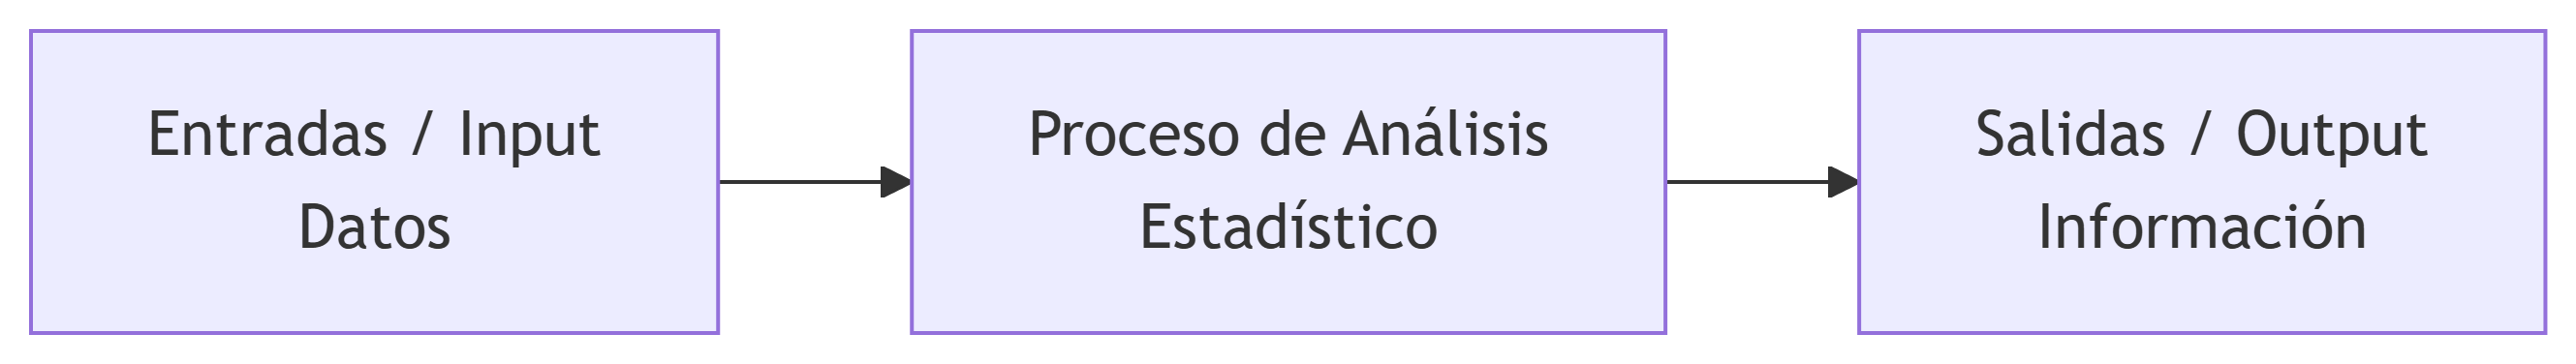
\includegraphics[width=6.93in,height=0.98in]{04_estadistica_descriptiva_files/figure-latex/mermaid-figure-1.png}

Enfoque sistémico del análisis estadístico

Esta información se integra dentro del proceso de investigación
cuantitativa para generar o actualizar conocimiento en contextos de
incertidumbre. El proceso forma un ciclo de retroalimentación continua
mediante la contrastación (validación, ampliación, modificación o
refutación del conocimiento previo).

\begin{figure}[H]

{\centering \pandocbounded{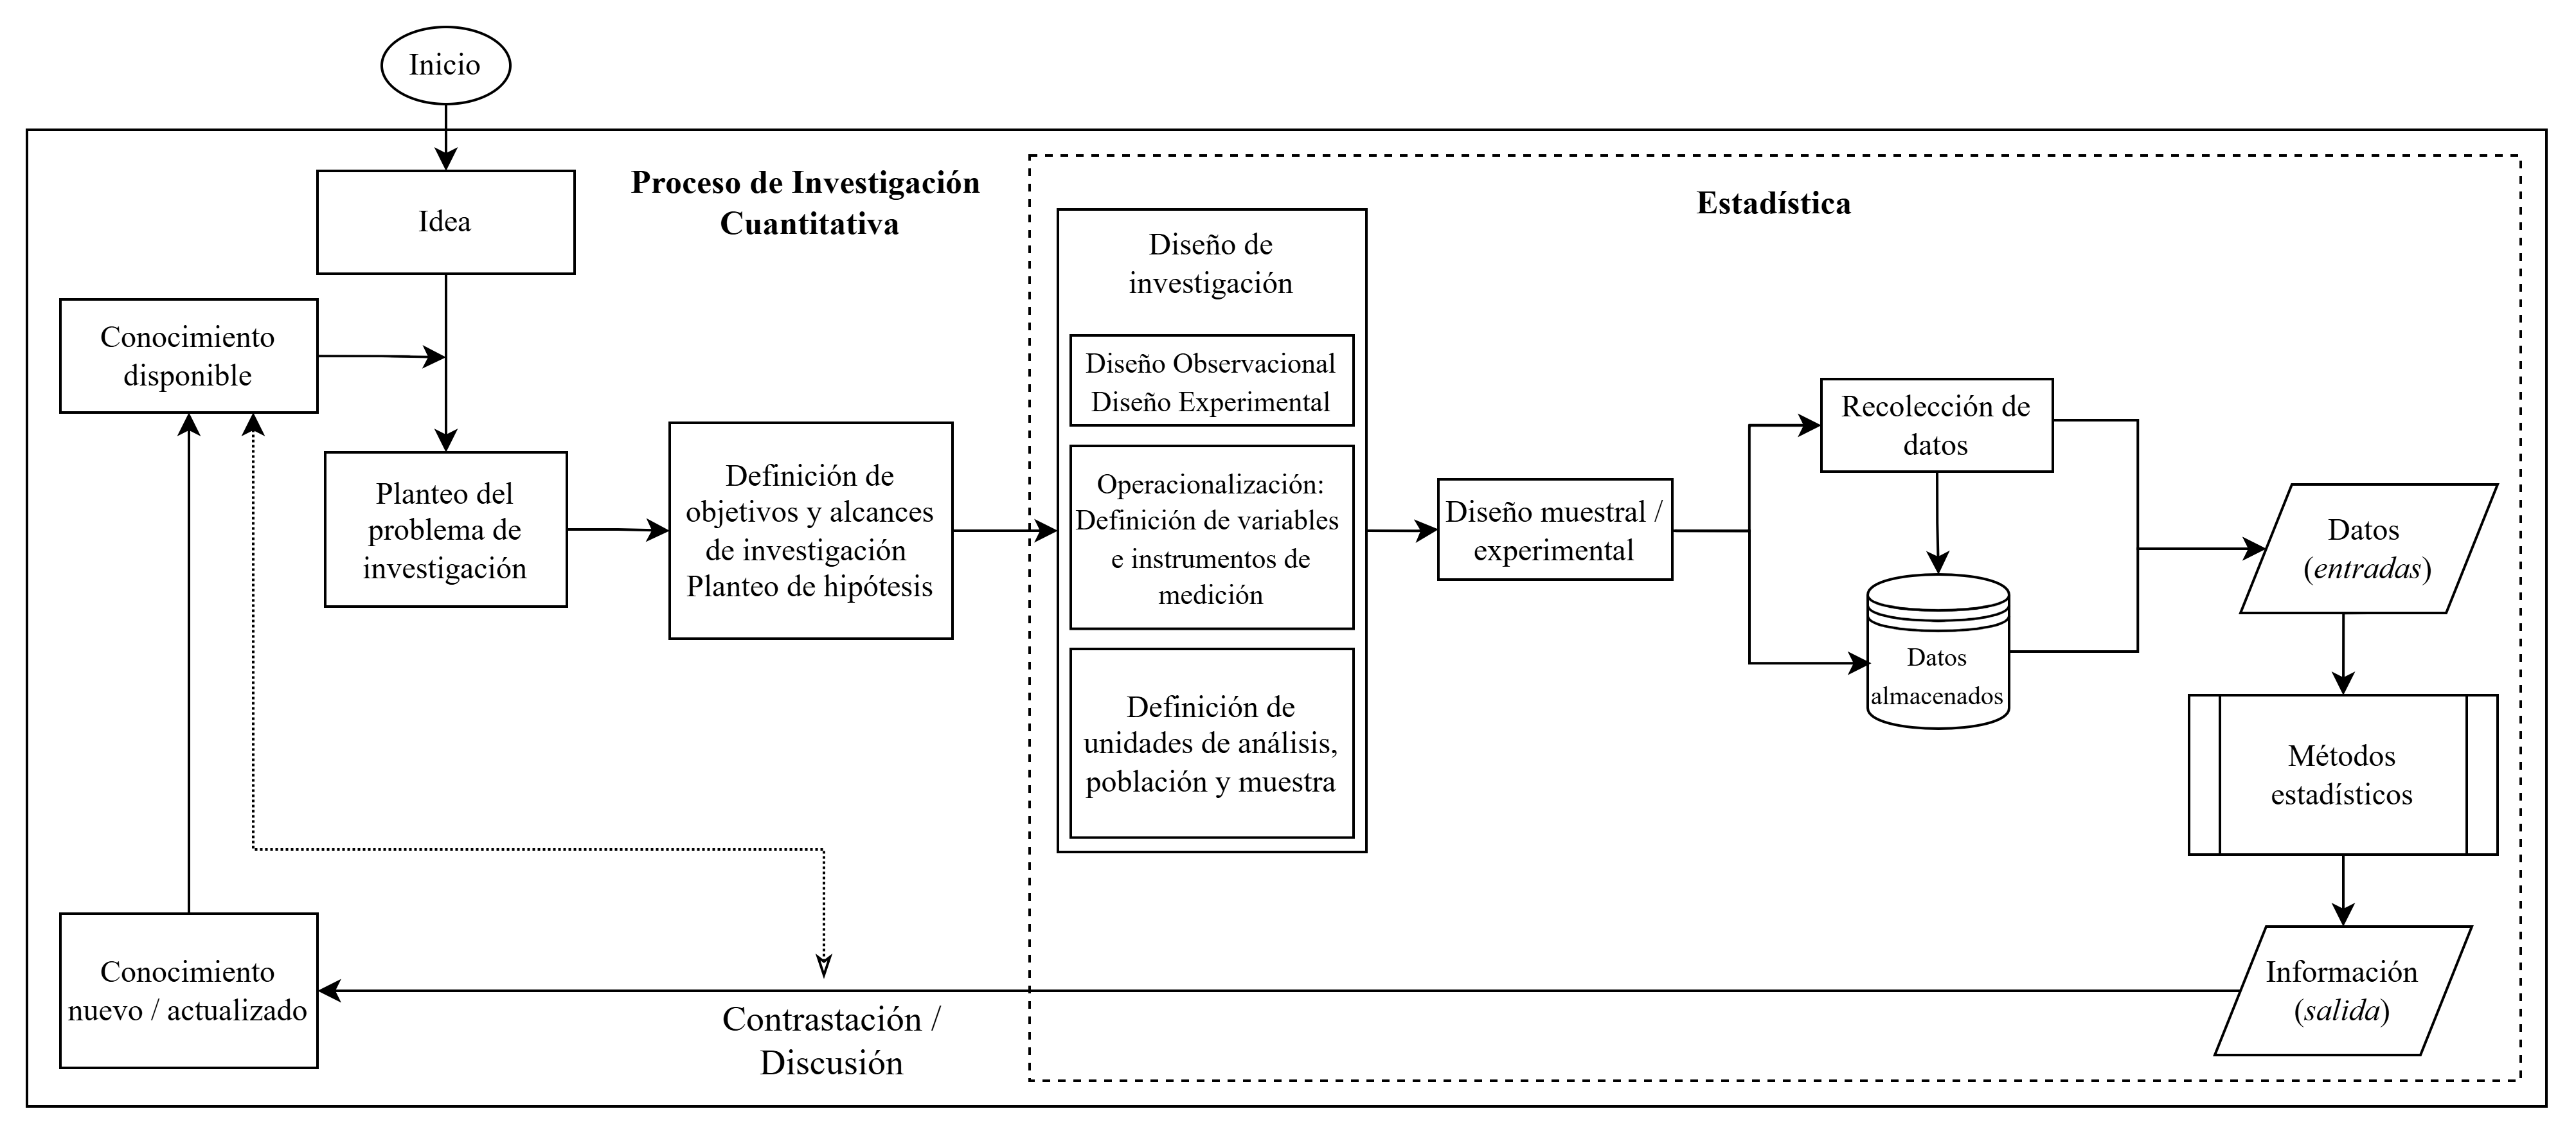
\includegraphics[keepaspectratio]{IMAGENES/2_INTRODUCCIÓN/Estadística dentro del proceso de investigación cuantitativa.jpg}}

}

\caption{Estadística dentro del proceso de investigación cuantitativa}

\end{figure}%

Desde un punto de vista \textbf{conceptual}, la estadística es la
ciencia que permite \textbf{aprender de los datos en contextos de
incertidumbre}. Su objetivo central es aislar la «señal» del «ruido»
mediante la \textbf{modelación estadística}.

\texttt{Modelo\ Estadístico}: Representación matemática con componentes
determinísticos y aleatorios para describir un proceso generador de
datos, basado en ciertos supuestos acerca de dicho proceso.

\section{Tipos de Problemas de Aprendizaje a partir de
Datos}\label{tipos-de-problemas-de-aprendizaje-a-partir-de-datos}

Según Vapnik (2000), el aprendizaje a partir de datos abarca tres tipos
de problemas:

\begin{enumerate}
\def\labelenumi{\arabic{enumi}.}
\tightlist
\item
  \textbf{Reconocimiento de patrones:} Identificación de regularidades o
  características significativas para clasificar o categorizar
  observaciones.
\item
  \textbf{Estimaciones por regresión:} Uso de relaciones matemáticas
  para predecir valores de una variable dependiente o realizar
  contrastes de hipótesis.
\item
  \textbf{Estimaciones de densidad:} Estimación de la probabilidad de
  ocurrencia de diferentes valores en un rango determinado.
\end{enumerate}

\subsection{Criterios de Clasificación de la Información
Estadística}\label{criterios-de-clasificaciuxf3n-de-la-informaciuxf3n-estaduxedstica}

La naturaleza de la información generada depende de los siguientes
factores:

\begin{itemize}
\tightlist
\item
  \textbf{Objetivos de la investigación:}

  \begin{itemize}
  \tightlist
  \item
    \textbf{Estadística Exploratoria / Descriptiva:} Busca descubrir
    relaciones o describir comportamientos de datos disponibles sin
    generalizar por fuera de la muestra.
  \item
    \textbf{Estadística Inferencial:} Permite contrastar hipótesis,
    estimar parámetros poblacionales o ajustar modelos generalizables.
    Incluye métodos \emph{explicativos} (mecanismos causales) y
    \emph{predictivos} (pronósticos).
  \end{itemize}
\item
  \textbf{Tipo de investigación (intervención):}

  \begin{itemize}
  \tightlist
  \item
    \textbf{Experimental:} Intervención activa y deliberada; describe
    relaciones de causa/efecto.
  \item
    \textbf{Observacional:} Sin intervención activa; describe
    asociaciones entre variables.
  \item
    \textbf{Semiexperimental:} Combina elementos observacionales y
    experimentales.
  \end{itemize}
\item
  \textbf{Naturaleza de la variable respuesta:}

  \begin{itemize}
  \tightlist
  \item
    \textbf{Respuesta numérica:} Requiere modelos de regresión
    (paramétricos o no paramétricos).
  \item
    \textbf{Respuesta categórica:} Requiere modelos de clasificación
    (métodos no paramétricos).
  \end{itemize}
\item
  \textbf{Número de variables analizadas:} Univariados, bivariados y
  multivariados.
\item
  \textbf{Relación Datos - Modelo - Predicción:}

  \begin{itemize}
  \tightlist
  \item
    \textbf{Inductivo/Inferencial:} Datos empíricos \(\rightarrow\)
    Regla general / Modelo teórico.
  \item
    \textbf{Deductivo:} Modelo teórico \(\rightarrow\) Evaluación de
    plausibilidad de predicciones.
  \item
    \textbf{Transductivo/Predictivo:} Datos empíricos \(\rightarrow\)
    Predicciones directas.
  \end{itemize}
\end{itemize}

\begin{figure}

\centering{

\pandocbounded{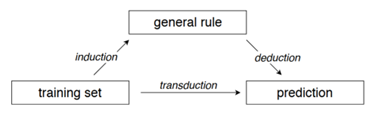
\includegraphics[keepaspectratio]{IMAGENES/2_INTRODUCCIÓN/enfoques.jpg}}

}

\caption{\label{fig-enfoques}Enfoques inductivo, deductivo y
transductivo}

\end{figure}%

\begin{figure}

\centering{

\pandocbounded{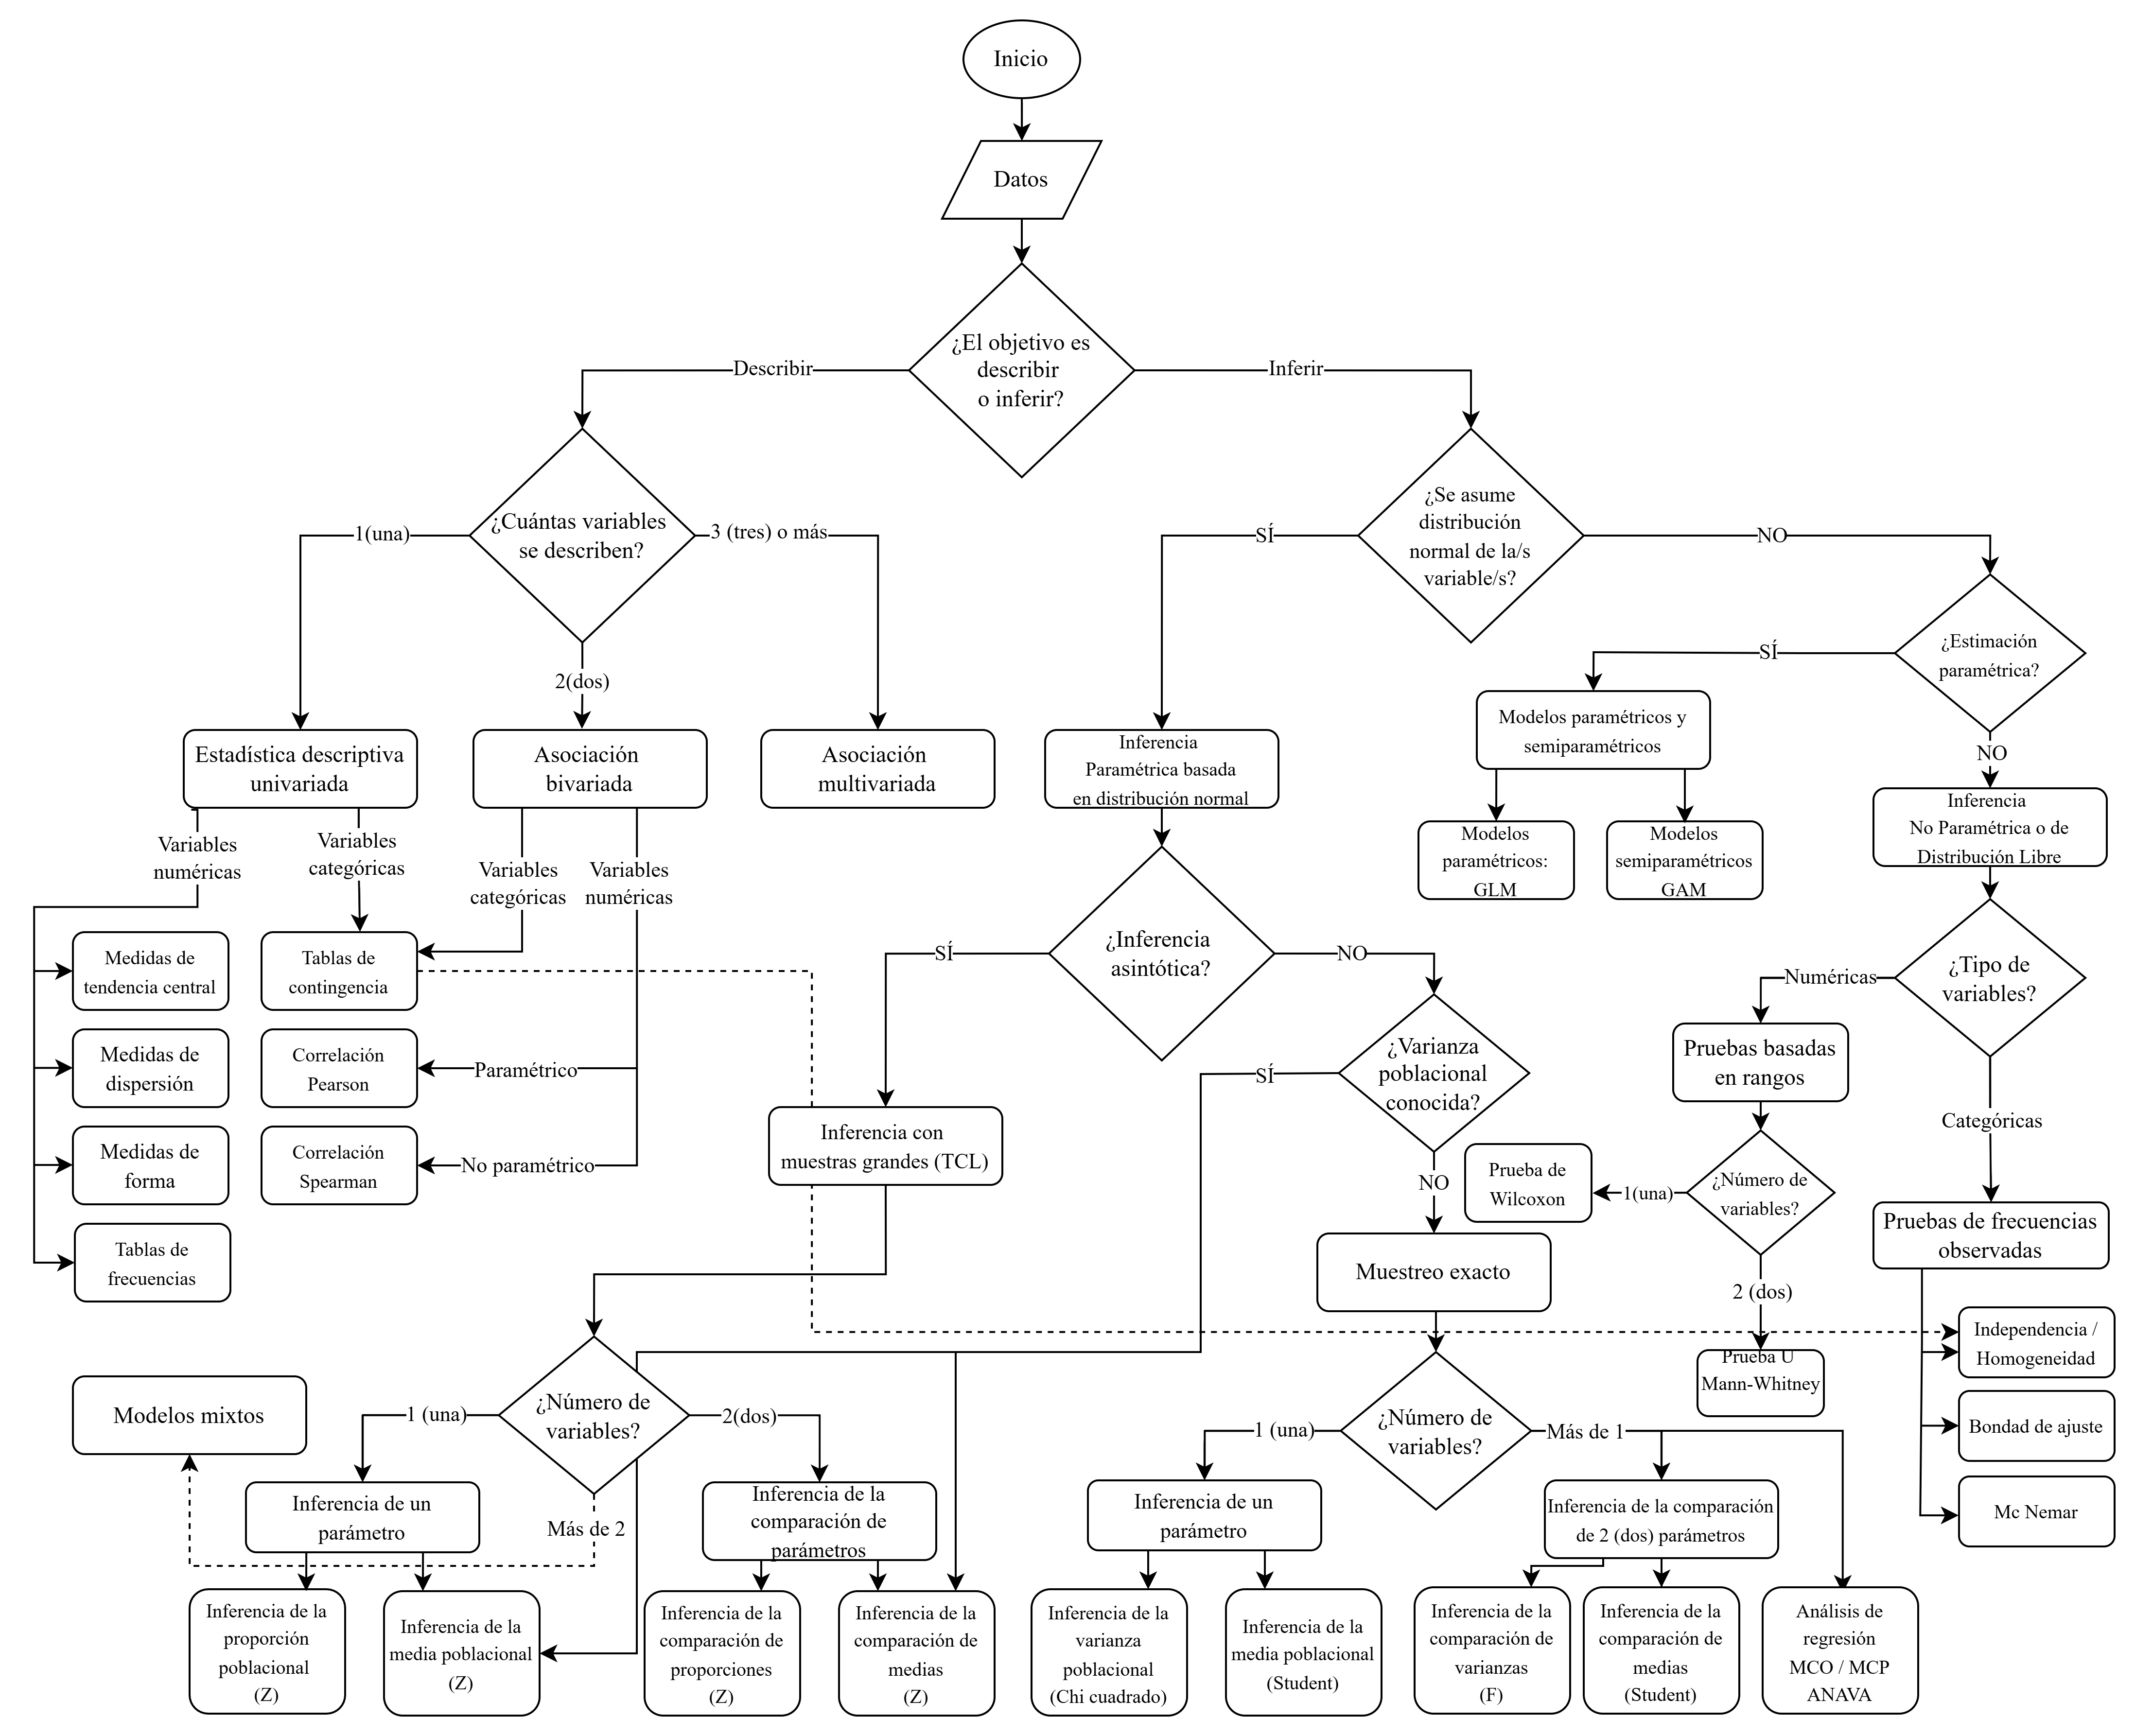
\includegraphics[keepaspectratio]{IMAGENES/2_INTRODUCCIÓN/Proceso de selección de métodos de análisis estadístico.jpg}}

}

\caption{\label{fig-seleccion-metodos}Proceso de selección de métodos de
análisis estadístico}

\end{figure}%

\subsection{Bioestadística}\label{bioestaduxedstica}

La \textbf{Bioestadística} es la rama que estudia los criterios para la
aplicación adecuada de los métodos estadísticos en las ciencias
biológicas, agrícolas, ambientales y de la salud, caracterizadas por la
elevada complejidad y variabilidad de los fenómenos biológicos.

\begin{center}\rule{0.5\linewidth}{0.5pt}\end{center}

\section{Población y Muestra}\label{poblaciuxf3n-y-muestra}

\subsection{Conceptos}\label{conceptos}

\begin{itemize}
\tightlist
\item
  \textbf{Población:} Conjunto de elementos acotados en un tiempo y
  espacio determinados, con alguna característica común observable o
  medible. Se delimita formalmente para definir el alcance de la
  inferencia.
\item
  \textbf{Tamaño Poblacional (}\(N\)): Número total de elementos de la
  población.
\item
  \textbf{Muestra:} Subconjunto representativo de la población.
\item
  \textbf{Tamaño Muestral (}\(n\)): Número de elementos incluidos en la
  muestra.
\end{itemize}

\subsection{Tipos de Poblaciones y
Muestreo}\label{tipos-de-poblaciones-y-muestreo}

\begin{itemize}
\tightlist
\item
  \textbf{Población Finita:} Aquella cuyos elementos constitutivos
  pueden ser contados y es posible determinar \(N\).
\item
  \textbf{Población Infinita:} Aquella en la que no es posible
  determinar el número total \(N\) mediante conteo.
\item
  \textbf{Muestreo Probabilístico vs.~Oportunista:} Para garantizar
  representatividad y medir el error de estimación se requieren métodos
  probabilísticos mediante marcos muestrales; no obstante, en biología
  se recurre frecuentemente a muestreos oportunistas por restricciones
  prácticas.
\end{itemize}

\subsection{Unidades de Estudio}\label{unidades-de-estudio}

\begin{itemize}
\tightlist
\item
  \textbf{Unidad de Observación (U.O.):} Elemento individual en la
  muestra sobre el cual se realiza la medición, conteo o clasificación.
\item
  \textbf{Unidad de Análisis (U.A.):} Objeto final del estudio sobre el
  cual se extraen las conclusiones inferenciales.
\end{itemize}

\begin{tcolorbox}[enhanced jigsaw, arc=.35mm, bottomrule=.15mm, bottomtitle=1mm, breakable, colback=white, colbacktitle=quarto-callout-note-color!10!white, colframe=quarto-callout-note-color-frame, coltitle=black, left=2mm, leftrule=.75mm, opacityback=0, opacitybacktitle=0.6, rightrule=.15mm, title=\textcolor{quarto-callout-note-color}{\faInfo}\hspace{0.5em}{Nota}, titlerule=0mm, toprule=.15mm, toptitle=1mm]

La Unidad de Observación (U.O.) y la Unidad de Análisis (U.A.) pueden o
no coincidir según el diseño muestral.

\end{tcolorbox}

\begin{center}\rule{0.5\linewidth}{0.5pt}\end{center}

\section{Variables Estadísticas y Escalas de
Medición}\label{variables-estaduxedsticas-y-escalas-de-mediciuxf3n}

\subsection{Definiciones}\label{definiciones}

\begin{itemize}
\tightlist
\item
  \textbf{Variable:} Característica o atributo que puede adoptar
  distintos valores numéricos o categóricos a partir de un conjunto de
  valores posibles. Se denota con letras mayúsculas (\(X, Y\)).
\item
  \textbf{Realización / Dato (}\(x_i\)): Valor específico que asume la
  variable en una unidad de observación (\(x_i, i=1, 2, \dots, n\)).
\item
  \textbf{Constante:} Atributo cuyo valor permanece invariante entre las
  unidades observadas.
\end{itemize}

\subsection{Clasificación por Naturaleza y Escala de
Medición}\label{clasificaciuxf3n-por-naturaleza-y-escala-de-mediciuxf3n}

\begin{figure}

\centering{

\pandocbounded{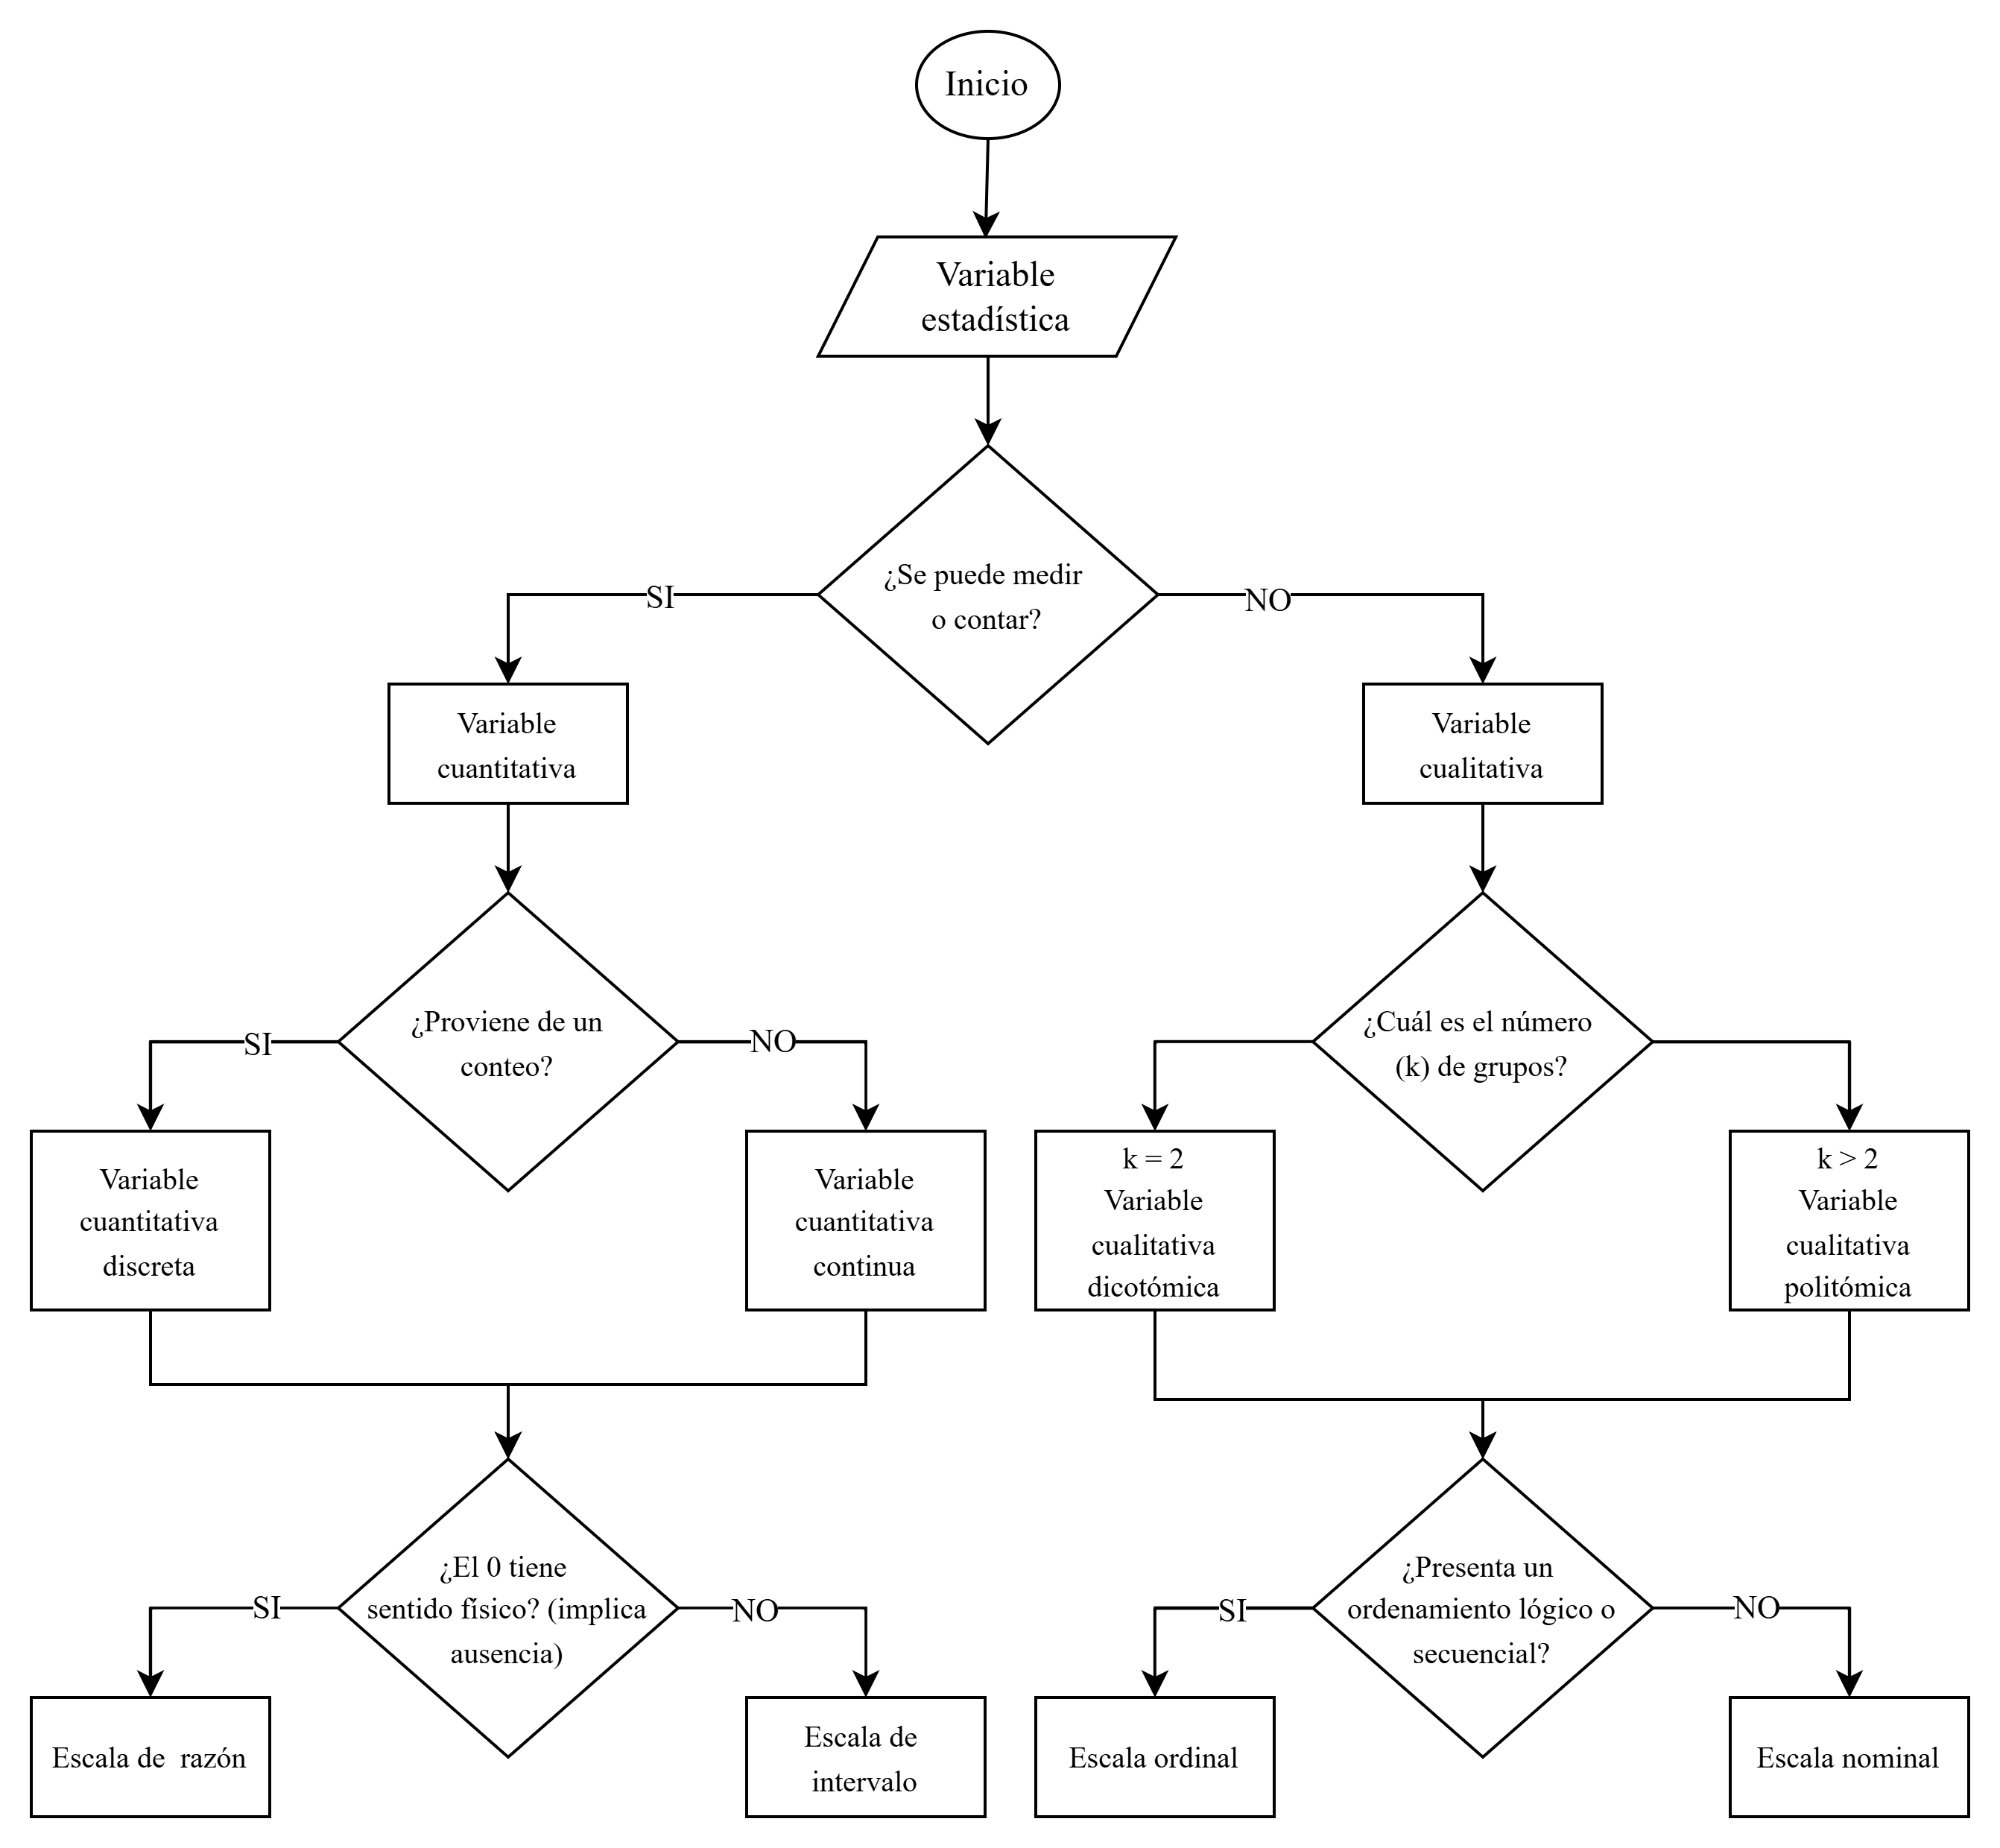
\includegraphics[keepaspectratio]{IMAGENES/2_INTRODUCCIÓN/Clasificación de variables estadísticas.jpg}}

}

\caption{\label{fig-clasificacion-variables}Clasificación de variables
estadísticas}

\end{figure}%

\subsubsection{Atributos de las Escalas de
Medición}\label{atributos-de-las-escalas-de-mediciuxf3n}

{\def\LTcaptype{none} % do not increment counter
\begin{longtable}[]{@{}
  >{\raggedright\arraybackslash}p{(\linewidth - 4\tabcolsep) * \real{0.3333}}
  >{\raggedright\arraybackslash}p{(\linewidth - 4\tabcolsep) * \real{0.3333}}
  >{\raggedright\arraybackslash}p{(\linewidth - 4\tabcolsep) * \real{0.3333}}@{}}
\toprule\noalign{}
\begin{minipage}[b]{\linewidth}\raggedright
Escala
\end{minipage} & \begin{minipage}[b]{\linewidth}\raggedright
Propiedades Operativas
\end{minipage} & \begin{minipage}[b]{\linewidth}\raggedright
Definición
\end{minipage} \\
\midrule\noalign{}
\endhead
\bottomrule\noalign{}
\endlastfoot
\textbf{Nominal} & Clasificación & Clasifica en categorías mutuamente
excluyentes sin orden implícito. \\
\textbf{Ordinal} & Clasificación, Orden & Establece un orden lógico o
jerarquía entre categorías, pero no mide distancias. \\
\textbf{Intervalo} & Clasificación, Orden, Distancia & Medición numérica
con cero arbitrario (no indica ausencia del atributo). \\
\textbf{Razón} & Clasificación, Orden, Distancia, Origen & Medición
numérica con cero real (ausencia del atributo); admite todas las
operaciones matemáticas. \\
\end{longtable}
}

\begin{center}\rule{0.5\linewidth}{0.5pt}\end{center}

\section{Estadística Descriptiva}\label{estaduxedstica-descriptiva}

Su objetivo es sintetizar y caracterizar los atributos de
\textbf{centralidad, variabilidad y forma} de la distribución de los
datos empíricos.

\begin{figure}

\centering{

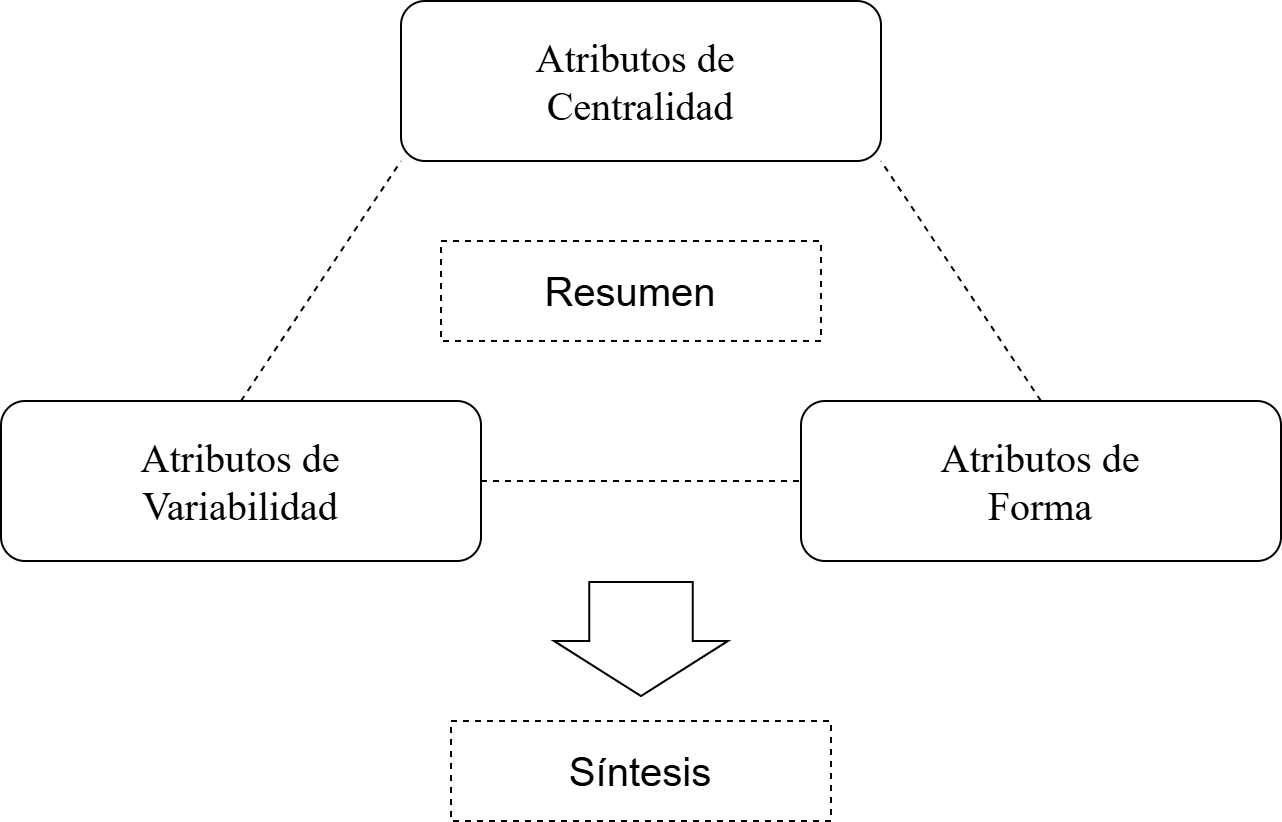
\includegraphics[width=0.8\linewidth,height=\textheight,keepaspectratio]{IMAGENES/3_ESTADÍSTICA DESCRIPTIVA/descriptiva_sintesis.jpg}

}

\caption{\label{fig-atributos-datos}Tipos de atributos para describir
datos empíricos}

\end{figure}%

\begin{figure}

\centering{

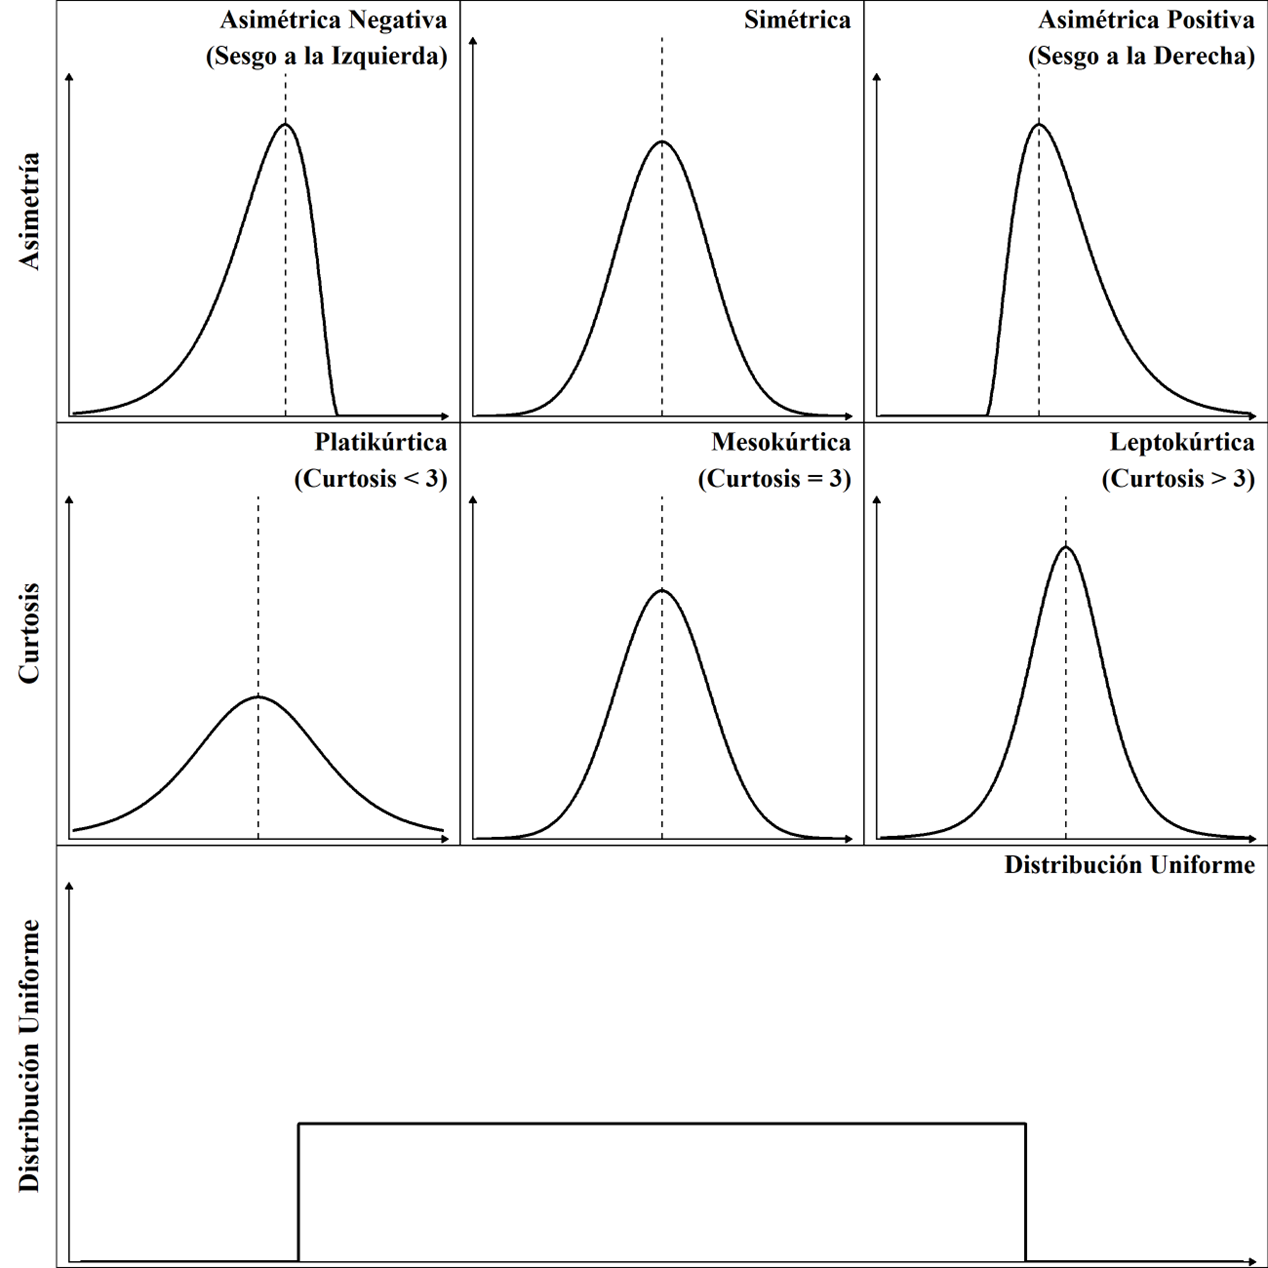
\includegraphics[width=0.8\linewidth,height=\textheight,keepaspectratio]{IMAGENES/3_ESTADÍSTICA DESCRIPTIVA/Ejemplos de algunas formas características.jpg}

}

\caption{\label{fig-formas-distribuciones}Ejemplos de algunas formas
características de distribuciones}

\end{figure}%

\begin{center}\rule{0.5\linewidth}{0.5pt}\end{center}

\section{Análisis Exploratorio de Series Simples y
Agrupadas}\label{anuxe1lisis-exploratorio-de-series-simples-y-agrupadas}

Realizar una lactura complementaria de la Unidad 3 del libro
\texttt{Apuntes\ de\ Bioestadística.\ Con\ ejercicios\ resueltos}.

\section{Estrategias de interacción con la
IA}\label{estrategias-de-interacciuxf3n-con-la-ia}

\begin{tcolorbox}[enhanced jigsaw, arc=.35mm, bottomrule=.15mm, bottomtitle=1mm, breakable, colback=white, colbacktitle=quarto-callout-tip-color!10!white, colframe=quarto-callout-tip-color-frame, coltitle=black, left=2mm, leftrule=.75mm, opacityback=0, opacitybacktitle=0.6, rightrule=.15mm, title=\textcolor{quarto-callout-tip-color}{\faLightbulb}\hspace{0.5em}{Estrategias de interacción con la IA}, titlerule=0mm, toprule=.15mm, toptitle=1mm]

\begin{itemize}
\tightlist
\item
  Dilema del número de clases: Pedir a la IA que compare los resultados
  del número de clases para cualquier serie de 30 valores utilizando los
  métodos de Sturges, Scott y Freedman-Diaconis. Preguntar: ``¿En qué
  situaciones preferiríamos una distribución más `suavizada' (Sturges)
  frente a una que resalte más los picos de variabilidad local?''.
\item
  Contraste de precisión (Muestra simple vs.~Agrupada): Solicitar a la
  IA que explique por qué existe una diferencia (aunque sea mínima)
  entre la media aritmética de la serie simple y la media ponderada
  calculada a partir de las marcas de clase. Reflexionar sobre el
  concepto de que la marca de clase ``asume'' que los datos se
  distribuyen uniformemente dentro del intervalo.
\item
  Razonamiento sobre la Mediana por Interpolación: Presentar a la IA la
  fórmula de interpolación para la mediana en variables continuas y
  pedirle que explique, mediante una analogía física, qué representan
  los componentes y por qué se multiplican por la amplitud.
\item
  Gráficos acumulados: Solicitar a la IA que justifique por qué una
  variable discreta (como el recuento de huevos de barrenador) debe
  graficarse con un gráfico escalonado que muestre saltos o
  discontinuidades, mientras que una variable continua (como el
  arsénico) permite una ojiva de líneas rectas que asumen una transición
  suave entre límites.
\item
  Análisis de la Moda en intervalos: Debatir con la IA sobre la
  sensibilidad de la clase modal. Preguntar: ``Si cambiamos la amplitud
  de los intervalos en el ejemplo de arsénico en Tumbaya, ¿podría la
  moda desplazarse de intervalo? ¿Qué nos dice esto sobre la estabilidad
  de esta medida en datos agrupados?''.
\item
  Simulación de sesgos por intervalos: Pedir a la IA que genere un
  escenario donde un investigador ``manipula'' visualmente un histograma
  aumentando excesivamente el número de clases hasta que cada barra
  tenga frecuencia 1, y discutir por qué esto anula el propósito del
  análisis de series agrupadas.
\item
  Traducción de algoritmos de software: Preguntar a la IA cómo el
  argumento breaks en la función hist() de R o la opción de ``Número de
  clases personalizado'' en InfoStat afectan el cálculo automático de
  las frecuencias, comparándolo con el procedimiento manual.
\end{itemize}

\end{tcolorbox}

\section{Micro-ejercicios de aplicación
(optativos)}\label{micro-ejercicios-de-aplicaciuxf3n-optativos-1}

Los siguientes micro-ejercicios te permitirán practicar los conceptos
revisados en esta unidad. Puedes copiar y pegar las preguntas en un
script de R local, o bien utilizar \texttt{webR}, que es la versión
\emph{online} de R, disponible en esta guía.

\texttt{Nota}: los ejercicios están inspirados en trabajos científicos
publicados, pero contienen datos simulados. Por lo tanto, los resultados
obtenidos deben interpretarse únicamente con fines didácticos y no como
evidencia científica.

La finalidad es familiarizarse con el análisis estadístico y con el uso
de R a partir de situaciones similares a las que pueden encontrarse en
investigaciones reales.

\begin{Shaded}
\begin{Highlighting}[]


\CommentTok{\# =============================================================================}
\CommentTok{\# MICRO{-}EJERCICIOS OPTATIVOS — Estadística Descriptiva}
\CommentTok{\# =============================================================================}

\CommentTok{\# {-}{-}{-}{-}{-}{-}{-}{-}{-}{-}{-}{-}{-}{-}{-}{-}{-}{-}{-}{-}{-}{-}{-}{-}{-}{-}{-}{-}{-}{-}{-}{-}{-}{-}{-}{-}{-}{-}{-}{-}{-}{-}{-}{-}{-}{-}{-}{-}{-}{-}{-}{-}{-}{-}{-}{-}{-}{-}{-}{-}{-}{-}{-}{-}{-}{-}{-}{-}{-}{-}{-}{-}{-}{-}{-}{-}{-}}
\CommentTok{\# I. POBLACIÓN, MUESTRA Y UNIDAD DE ANÁLISIS}
\CommentTok{\# {-}{-}{-}{-}{-}{-}{-}{-}{-}{-}{-}{-}{-}{-}{-}{-}{-}{-}{-}{-}{-}{-}{-}{-}{-}{-}{-}{-}{-}{-}{-}{-}{-}{-}{-}{-}{-}{-}{-}{-}{-}{-}{-}{-}{-}{-}{-}{-}{-}{-}{-}{-}{-}{-}{-}{-}{-}{-}{-}{-}{-}{-}{-}{-}{-}{-}{-}{-}{-}{-}{-}{-}{-}{-}{-}{-}{-}}

\CommentTok{\# 1) Contexto: En la Reserva de Biosfera Laguna de Pozuelos habita una población}
\CommentTok{\#    de aproximadamente 800 vicuñas (Vicugna vicugna). Durante una jornada de}
\CommentTok{\#    esquila comunitaria (chaku) se arrean y capturan 40 individuos para medir}
\CommentTok{\#    el diámetro de su fibra.}
\CommentTok{\#    a) Identifique la población en estudio.}
\CommentTok{\#    b) Identifique la muestra y su tamaño (n).}
\CommentTok{\#    c) Identifique la unidad de análisis.}
\CommentTok{\#    Comente.}


\CommentTok{\# 2) Contexto: Un equipo de investigación releva la altura de individuos de cardón}
\CommentTok{\#    (Trichocereus atacamensis) en un sector de la Quebrada de Humahuaca que}
\CommentTok{\#    contiene aproximadamente 1200 ejemplares. Se seleccionan al azar 60}
\CommentTok{\#    individuos para la medición.}
\CommentTok{\#    a) Identifique la población y la muestra.}
\CommentTok{\#    b) Identifique la unidad observacional.}
\CommentTok{\#    Comente.}



\CommentTok{\# 3) Contexto: Se estudia el ataque de una plaga sobre cultivos de papa andina}
\CommentTok{\#    (Solanum tuberosum ssp. andigena) en la Quebrada de Humahuaca. De un total}
\CommentTok{\#    de 300 hectáreas cultivadas, un técnico selecciona 12 parcelas y, dentro}
\CommentTok{\#    de cada una, examina 20 plantas.}
\CommentTok{\#    a) Identifique la población en estudio.}
\CommentTok{\#    b) Identifique la unidad de análisis y la unidad observacional.}
\CommentTok{\#    c) Indique si la variable de interés surge a nivel de parcela o de planta.}
\CommentTok{\#    Comente.}


\CommentTok{\# 4) Contexto: Un equipo de limnología estudia la calidad del agua de los}
\CommentTok{\#    bofedales altoandinos de la cuenca de la Laguna de Pozuelos. De un total de 25}
\CommentTok{\#    bofedales en la cuenca, se seleccionan 8 al azar y se mide el pH del agua}
\CommentTok{\#    en cada uno.}
\CommentTok{\#    a) Identifique la población y la muestra.}
\CommentTok{\#    b) Identifique la unidad de análisis.}
\CommentTok{\#    Comente.}


\CommentTok{\# 5) Contexto: Un investigador afirma:}
\CommentTok{\#    "Coloqué 5 cámaras trampa en el Parque Nacional Calilegua y cada cámara}
\CommentTok{\#    registró en promedio 15 fotografías de puma (Puma concolor) durante el}
\CommentTok{\#    mes, por lo tanto mi tamaño muestral es n = 75."}
\CommentTok{\#    a) Analice la afirmación del investigador.}
\CommentTok{\#    b) Identifique cuál es la verdadera unidad de análisis del estudio.}
\CommentTok{\#    c) Explique la consecuencia de confundir las fotografías repetidas de un}
\CommentTok{\#       mismo individuo (pseudorréplicas) con el tamaño muestral real.}
\CommentTok{\#    Comente.}


\CommentTok{\# 6) Contexto: Se evalúa el efecto de la clausura al pastoreo sobre la}
\CommentTok{\#    regeneración de bosques de queñoa (Polylepis australis) en lel Bosque Montano}
\CommentTok{\#    de las Yungas Jujeñas. Un investigador instala 5 parcelas clausuradas y, dentro de cada}
\CommentTok{\#    una, cuenta el número de plantines en 4 subparcelas de 1 m².}
\CommentTok{\#    a) ¿Cuál es la unidad de análisis correcta: la parcela clausurada o la}
\CommentTok{\#       subparcela?}
\CommentTok{\#    b) Explique por qué tratar cada subparcela como una réplica independiente}
\CommentTok{\#       podría subestimar la variabilidad real del estudio.}
\CommentTok{\#    Comente.}


\CommentTok{\# {-}{-}{-}{-}{-}{-}{-}{-}{-}{-}{-}{-}{-}{-}{-}{-}{-}{-}{-}{-}{-}{-}{-}{-}{-}{-}{-}{-}{-}{-}{-}{-}{-}{-}{-}{-}{-}{-}{-}{-}{-}{-}{-}{-}{-}{-}{-}{-}{-}{-}{-}{-}{-}{-}{-}{-}{-}{-}{-}{-}{-}{-}{-}{-}{-}{-}{-}{-}{-}{-}{-}{-}{-}{-}{-}{-}{-}}
\CommentTok{\# II. ESCALAS DE MEDICIÓN}
\CommentTok{\# {-}{-}{-}{-}{-}{-}{-}{-}{-}{-}{-}{-}{-}{-}{-}{-}{-}{-}{-}{-}{-}{-}{-}{-}{-}{-}{-}{-}{-}{-}{-}{-}{-}{-}{-}{-}{-}{-}{-}{-}{-}{-}{-}{-}{-}{-}{-}{-}{-}{-}{-}{-}{-}{-}{-}{-}{-}{-}{-}{-}{-}{-}{-}{-}{-}{-}{-}{-}{-}{-}{-}{-}{-}{-}{-}{-}{-}}

\CommentTok{\# 7) Contexto: En un estudio de termorregulación de Liolaemus sp. en la Puna,}
\CommentTok{\#    se registra la temperatura corporal de un individuo asoleándose: 15 °C}
\CommentTok{\#    en la mañana y 30 °C al mediodía.}
\CommentTok{\#    Situación: un estudiante afirma: "El lagarto tiene exactamente el doble}
\CommentTok{\#    de temperatura corporal al mediodía que en la mañana."}
\CommentTok{\#    Comente.}


\CommentTok{\# 8) Contexto: Se mide la precipitación anual (mm) en dos sitios del NOA: uno}
\CommentTok{\#    recibe 400 mm y otro 800 mm.}
\CommentTok{\#    Situación: un investigador afirma: "El segundo sitio recibe exactamente}
\CommentTok{\#    el doble de precipitación que el primero."}
\CommentTok{\#    a) Comente si esta afirmación es válida.}
\CommentTok{\#    b) Compare con el caso de la temperatura en °C del ejercicio anterior:}
\CommentTok{\#       ¿por qué en este caso sí es correcto hablar de "el doble"?}


\CommentTok{\# 9) Contexto: Se clasifica el estado de conservación de poblaciones de}
\CommentTok{\#    Vultur gryphus según las categorías de la UICN: Preocupación menor,}
\CommentTok{\#    Casi amenazada, Vulnerable, En peligro, En peligro crítico.}
\CommentTok{\#    Situación: un investigador afirma: "Una población \textquotesingle{}En peligro crítico\textquotesingle{}}
\CommentTok{\#    está exactamente el doble de amenazada que una \textquotesingle{}Vulnerable\textquotesingle{}."}
\CommentTok{\#    Comente.}


\CommentTok{\# 10) Contexto: Se registra el tipo de cobertura vegetal dominante en sitios}
\CommentTok{\#     de muestreo de la Puna jujeña: Pastizal, Bofedal, Roquedal.}
\CommentTok{\#     Situación: un estudiante afirma: "El bofedal representa un nivel de}
\CommentTok{\#     cobertura mayor que el roquedal."}
\CommentTok{\#     Comente, identificando la escala de medición de la variable.}


\CommentTok{\# {-}{-}{-}{-}{-}{-}{-}{-}{-}{-}{-}{-}{-}{-}{-}{-}{-}{-}{-}{-}{-}{-}{-}{-}{-}{-}{-}{-}{-}{-}{-}{-}{-}{-}{-}{-}{-}{-}{-}{-}{-}{-}{-}{-}{-}{-}{-}{-}{-}{-}{-}{-}{-}{-}{-}{-}{-}{-}{-}{-}{-}{-}{-}{-}{-}{-}{-}{-}{-}{-}{-}{-}{-}{-}{-}{-}{-}}
\CommentTok{\# III. SERIES SIMPLES — MEDIDAS DE RESUMEN}
\CommentTok{\# {-}{-}{-}{-}{-}{-}{-}{-}{-}{-}{-}{-}{-}{-}{-}{-}{-}{-}{-}{-}{-}{-}{-}{-}{-}{-}{-}{-}{-}{-}{-}{-}{-}{-}{-}{-}{-}{-}{-}{-}{-}{-}{-}{-}{-}{-}{-}{-}{-}{-}{-}{-}{-}{-}{-}{-}{-}{-}{-}{-}{-}{-}{-}{-}{-}{-}{-}{-}{-}{-}{-}{-}{-}{-}{-}{-}{-}}

\CommentTok{\# 11) Se midió la longitud del ala (mm) de 10 individuos de aguilucho común}
\CommentTok{\#     (Geranoaetus polyosoma) capturados:}

\NormalTok{ala\_aguilucho }\OtherTok{=} \FunctionTok{c}\NormalTok{(}\DecValTok{365}\NormalTok{, }\DecValTok{372}\NormalTok{, }\DecValTok{358}\NormalTok{, }\DecValTok{380}\NormalTok{, }\DecValTok{369}\NormalTok{, }\DecValTok{374}\NormalTok{, }\DecValTok{361}\NormalTok{, }\DecValTok{377}\NormalTok{, }\DecValTok{366}\NormalTok{, }\DecValTok{371}\NormalTok{)}

\CommentTok{\#     a) Identifique el tipo de variable y su escala de medición.}
\CommentTok{\#     b) Calcule la media y la mediana.}
\CommentTok{\#     c) Calcule el desvío estándar muestral.}
\CommentTok{\#     d) Interprete}
\CommentTok{\# Su código aquí:}


\CommentTok{\# 12) Se midió el diámetro medio (cm) de 8 individuos de yareta}
\CommentTok{\#     (Azorella compacta) en laderas rocosas de la Puna:}

\NormalTok{diametro\_yareta }\OtherTok{=} \FunctionTok{c}\NormalTok{(}\DecValTok{85}\NormalTok{, }\DecValTok{102}\NormalTok{, }\DecValTok{78}\NormalTok{, }\DecValTok{95}\NormalTok{, }\DecValTok{110}\NormalTok{, }\DecValTok{88}\NormalTok{, }\DecValTok{92}\NormalTok{, }\DecValTok{99}\NormalTok{)}

\CommentTok{\#     a) Calcule el coeficiente de variación (cv\_x) manualmente.}
\CommentTok{\#     b) Interprete si la muestra es homogénea o heterogénea.}
\CommentTok{\# Su código aquí:}


\CommentTok{\# 13) Se registró el peso (g) de 12 huevos de cóndor andino (Vultur gryphus)}
\CommentTok{\#     recolectados en un programa de cría en cautiverio:}

\NormalTok{peso\_huevo\_condor }\OtherTok{=} \FunctionTok{c}\NormalTok{(}\DecValTok{280}\NormalTok{, }\DecValTok{265}\NormalTok{, }\DecValTok{290}\NormalTok{, }\DecValTok{275}\NormalTok{, }\DecValTok{268}\NormalTok{, }\DecValTok{285}\NormalTok{, }\DecValTok{272}\NormalTok{, }\DecValTok{278}\NormalTok{, }\DecValTok{283}\NormalTok{, }\DecValTok{269}\NormalTok{, }\DecValTok{276}\NormalTok{, }\DecValTok{288}\NormalTok{)}

\CommentTok{\#     a) Calcule el rango (range()) y la amplitud (r\_x, manual).}
\CommentTok{\#     b) Calcule el primer y tercer cuartil con quantile().}
\CommentTok{\#     c) Interprete}
\CommentTok{\# Su código aquí:}


\CommentTok{\# 14) Se registró la duración (segundos) de despliegues territoriales de}
\CommentTok{\#     machos de Liolaemus sp. observados en la Quebrada de Humahuaca:}

\NormalTok{despliegue\_liolaemus }\OtherTok{=} \FunctionTok{c}\NormalTok{(}\DecValTok{8}\NormalTok{, }\DecValTok{12}\NormalTok{, }\DecValTok{6}\NormalTok{, }\DecValTok{15}\NormalTok{, }\DecValTok{9}\NormalTok{, }\DecValTok{11}\NormalTok{, }\DecValTok{7}\NormalTok{, }\DecValTok{14}\NormalTok{, }\DecValTok{10}\NormalTok{, }\DecValTok{13}\NormalTok{, }\DecValTok{9}\NormalTok{, }\DecValTok{16}\NormalTok{)}

\CommentTok{\#     a) Calcule la media y el desvío estándar.}
\CommentTok{\#     b) Calcule el coeficiente de asimetría con skewness() de \{moments\}.}
\CommentTok{\#     c) Interprete el signo del coeficiente obtenido.}
\CommentTok{\# Su código aquí:}


\CommentTok{\# 15) Se midió la concentración de oxígeno disuelto (mg/L) en 10 puntos de un}
\CommentTok{\#     arroyo de montaña de las Yungas jujeñas:}

\NormalTok{oxigeno\_arroyo }\OtherTok{=} \FunctionTok{c}\NormalTok{(}\FloatTok{7.2}\NormalTok{, }\FloatTok{6.8}\NormalTok{, }\FloatTok{7.5}\NormalTok{, }\FloatTok{6.9}\NormalTok{, }\FloatTok{7.1}\NormalTok{, }\FloatTok{8.0}\NormalTok{, }\FloatTok{6.5}\NormalTok{, }\FloatTok{7.8}\NormalTok{, }\FloatTok{7.0}\NormalTok{, }\FloatTok{7.4}\NormalTok{)}

\CommentTok{\#     a) Calcule la media y la mediana.}
\CommentTok{\#     b) Calcule la curtosis con kurtosis() de \{moments\}.}
\CommentTok{\#     c) Interprete el grado de concentración de los datos alrededor de la media.}
\CommentTok{\# Su código aquí:}


\CommentTok{\# 16) Se midió la longitud del pico (mm) de 9 individuos de picaflor puneño}
\CommentTok{\#     (Oreotrochilus sp.) capturados con red de niebla:}

\NormalTok{pico\_picaflor }\OtherTok{=} \FunctionTok{c}\NormalTok{(}\FloatTok{23.5}\NormalTok{, }\FloatTok{24.1}\NormalTok{, }\FloatTok{22.8}\NormalTok{, }\FloatTok{24.6}\NormalTok{, }\FloatTok{23.2}\NormalTok{, }\FloatTok{24.0}\NormalTok{, }\FloatTok{23.8}\NormalTok{, }\FloatTok{22.9}\NormalTok{, }\FloatTok{24.3}\NormalTok{)}

\CommentTok{\#     a) Aplique s\_simple() de \{resumiR\} para obtener todas las medidas de}
\CommentTok{\#        resumen de una vez.}
\CommentTok{\#     b) Identifique el valor del coeficiente de variación en la salida.}
\CommentTok{\#     c) Interprete}
\CommentTok{\# Su código aquí:}


\CommentTok{\# 17) Se registró el peso de fibra esquilada (g) por vicuña en una jornada de}
\CommentTok{\#     esquila comunitaria de la Puna jujeña:}

\NormalTok{fibra\_vicuna }\OtherTok{=} \FunctionTok{c}\NormalTok{(}\DecValTok{220}\NormalTok{, }\DecValTok{245}\NormalTok{, }\DecValTok{198}\NormalTok{, }\DecValTok{260}\NormalTok{, }\DecValTok{235}\NormalTok{, }\DecValTok{210}\NormalTok{, }\DecValTok{250}\NormalTok{, }\DecValTok{228}\NormalTok{, }\DecValTok{242}\NormalTok{, }\DecValTok{205}\NormalTok{, }\DecValTok{233}\NormalTok{, }\DecValTok{218}\NormalTok{)}

\CommentTok{\#     a) Calcule la media, la mediana y el desvío estándar.}
\CommentTok{\#     b) Calcule el cv\_x (manual) e interprete la homogeneidad del rendimiento}
\CommentTok{\#        de fibra en la jornada.}
\CommentTok{\# Su código aquí:}


\CommentTok{\# 18) Se midió la altura (m) de 10 individuos de queñoa (Polylepis australis)}
\CommentTok{\#     en un bosque relictual de la Puna:}

\NormalTok{altura\_quenoa\_bosque }\OtherTok{=} \FunctionTok{c}\NormalTok{(}\FloatTok{2.4}\NormalTok{, }\FloatTok{3.1}\NormalTok{, }\FloatTok{2.8}\NormalTok{, }\FloatTok{3.5}\NormalTok{, }\FloatTok{2.6}\NormalTok{, }\FloatTok{3.0}\NormalTok{, }\FloatTok{2.9}\NormalTok{, }\FloatTok{3.3}\NormalTok{, }\FloatTok{2.7}\NormalTok{, }\FloatTok{3.2}\NormalTok{)}

\CommentTok{\#     a) Calcule el cv\_x (manual).}
\CommentTok{\#     b) Compare mentalmente con el cv obtenido en el ejercicio 12 (yareta):}
\CommentTok{\#        ¿cuál de las dos especies presenta mayor variabilidad relativa?}
\CommentTok{\# Su código aquí:}


\CommentTok{\# {-}{-}{-}{-}{-}{-}{-}{-}{-}{-}{-}{-}{-}{-}{-}{-}{-}{-}{-}{-}{-}{-}{-}{-}{-}{-}{-}{-}{-}{-}{-}{-}{-}{-}{-}{-}{-}{-}{-}{-}{-}{-}{-}{-}{-}{-}{-}{-}{-}{-}{-}{-}{-}{-}{-}{-}{-}{-}{-}{-}{-}{-}{-}{-}{-}{-}{-}{-}{-}{-}{-}{-}{-}{-}{-}{-}{-}}
\CommentTok{\# IV. SERIES AGRUPADAS — VARIABLES CONTINUAS}
\CommentTok{\# {-}{-}{-}{-}{-}{-}{-}{-}{-}{-}{-}{-}{-}{-}{-}{-}{-}{-}{-}{-}{-}{-}{-}{-}{-}{-}{-}{-}{-}{-}{-}{-}{-}{-}{-}{-}{-}{-}{-}{-}{-}{-}{-}{-}{-}{-}{-}{-}{-}{-}{-}{-}{-}{-}{-}{-}{-}{-}{-}{-}{-}{-}{-}{-}{-}{-}{-}{-}{-}{-}{-}{-}{-}{-}{-}{-}{-}}

\CommentTok{\# 19) Se midió el pH del agua en 20 bofedales altoandinos de la cuenca de la}
\CommentTok{\#     Laguna de Pozuelos:}

\NormalTok{ph\_bofedales }\OtherTok{=} \FunctionTok{c}\NormalTok{(}\FloatTok{6.8}\NormalTok{, }\FloatTok{7.2}\NormalTok{, }\FloatTok{7.5}\NormalTok{, }\FloatTok{6.9}\NormalTok{, }\FloatTok{7.1}\NormalTok{, }\FloatTok{7.8}\NormalTok{, }\FloatTok{6.6}\NormalTok{, }\FloatTok{7.4}\NormalTok{, }\FloatTok{7.0}\NormalTok{, }\FloatTok{7.3}\NormalTok{,}
                  \FloatTok{6.7}\NormalTok{, }\FloatTok{7.6}\NormalTok{, }\FloatTok{7.2}\NormalTok{, }\FloatTok{6.9}\NormalTok{, }\FloatTok{7.5}\NormalTok{, }\FloatTok{7.1}\NormalTok{, }\FloatTok{6.8}\NormalTok{, }\FloatTok{7.7}\NormalTok{, }\FloatTok{7.0}\NormalTok{, }\FloatTok{7.3}\NormalTok{)}

\CommentTok{\#     a) Aplique s\_agrupada() de \{resumiR\} para construir la tabla de}
\CommentTok{\#        frecuencias por intervalos.}
\CommentTok{\#     b) Identifique el intervalo de clase más frecuente.}
\CommentTok{\# Su código aquí:}


\CommentTok{\# 20) Se midió el diámetro a la altura del pecho (DAP, cm) de 20 individuos de}
\CommentTok{\#     algarrobo negro (Prosopis nigra) en un relicto de bosque chaqueño:}

\NormalTok{dap\_algarrobo }\OtherTok{=} \FunctionTok{c}\NormalTok{(}\DecValTok{18}\NormalTok{, }\DecValTok{22}\NormalTok{, }\DecValTok{25}\NormalTok{, }\DecValTok{19}\NormalTok{, }\DecValTok{21}\NormalTok{, }\DecValTok{28}\NormalTok{, }\DecValTok{17}\NormalTok{, }\DecValTok{24}\NormalTok{, }\DecValTok{20}\NormalTok{, }\DecValTok{26}\NormalTok{,}
                   \DecValTok{19}\NormalTok{, }\DecValTok{23}\NormalTok{, }\DecValTok{27}\NormalTok{, }\DecValTok{18}\NormalTok{, }\DecValTok{22}\NormalTok{, }\DecValTok{25}\NormalTok{, }\DecValTok{20}\NormalTok{, }\DecValTok{24}\NormalTok{, }\DecValTok{21}\NormalTok{, }\DecValTok{26}\NormalTok{)}

\CommentTok{\#     a) Aplique s\_agrupada() y obtenga la tabla de frecuencias.}
\CommentTok{\#     b) Calcule la media y el desvío estándar a partir de la salida.}
\CommentTok{\# Su código aquí:}


\CommentTok{\# 21) Se midió la turbidez del agua (NTU) en 20 muestras de una laguna}
\CommentTok{\#     altoandina utilizada como bebedero de fauna silvestre:}

\NormalTok{turbidez\_laguna }\OtherTok{=} \FunctionTok{c}\NormalTok{(}\DecValTok{12}\NormalTok{, }\DecValTok{18}\NormalTok{, }\DecValTok{25}\NormalTok{, }\DecValTok{15}\NormalTok{, }\DecValTok{20}\NormalTok{, }\DecValTok{30}\NormalTok{, }\DecValTok{10}\NormalTok{, }\DecValTok{22}\NormalTok{, }\DecValTok{17}\NormalTok{, }\DecValTok{28}\NormalTok{,}
                     \DecValTok{14}\NormalTok{, }\DecValTok{24}\NormalTok{, }\DecValTok{19}\NormalTok{, }\DecValTok{11}\NormalTok{, }\DecValTok{26}\NormalTok{, }\DecValTok{16}\NormalTok{, }\DecValTok{21}\NormalTok{, }\DecValTok{13}\NormalTok{, }\DecValTok{27}\NormalTok{, }\DecValTok{23}\NormalTok{)}

\CommentTok{\#     a) Aplique s\_agrupada() y obtenga la tabla de frecuencias.}
\CommentTok{\#     b) A partir de la tabla, elabore una conclusión sobre la distribución de}
\CommentTok{\#        los datos.}
\CommentTok{\# Su código aquí:}


\CommentTok{\# 22) Se midió la temperatura corporal (°C) de 20 sapos andinos (Rhinella}
\CommentTok{\#     spinulosa) activos en un bofedal de la Puna jujeña:}

\NormalTok{temp\_corporal\_sapo }\OtherTok{=} \FunctionTok{c}\NormalTok{(}\FloatTok{13.5}\NormalTok{, }\FloatTok{15.2}\NormalTok{, }\FloatTok{16.8}\NormalTok{, }\FloatTok{14.1}\NormalTok{, }\FloatTok{15.5}\NormalTok{, }\FloatTok{17.2}\NormalTok{, }\FloatTok{12.9}\NormalTok{, }\FloatTok{16.0}\NormalTok{, }\FloatTok{14.5}\NormalTok{, }\FloatTok{17.5}\NormalTok{,}
                        \FloatTok{13.8}\NormalTok{, }\FloatTok{16.3}\NormalTok{, }\FloatTok{15.0}\NormalTok{, }\FloatTok{12.5}\NormalTok{, }\FloatTok{17.0}\NormalTok{, }\FloatTok{14.8}\NormalTok{, }\FloatTok{15.8}\NormalTok{, }\FloatTok{13.2}\NormalTok{, }\FloatTok{16.5}\NormalTok{, }\FloatTok{15.3}\NormalTok{)}

\CommentTok{\#     a) Aplique s\_agrupada() y obtenga la tabla de frecuencias.}
\CommentTok{\#     b) Identifique el intervalo modal de la distribución.}
\CommentTok{\# Su código aquí:}


\CommentTok{\# NOTA: EN TODOS LOS EJERCICIOS, CONSTRUYA EL HISTOGRAMA DE FRECUENCIAS Y EL }
\CommentTok{\# GRÁFICO DE OJIVA.}

\CommentTok{\# {-}{-}{-}{-}{-}{-}{-}{-}{-}{-}{-}{-}{-}{-}{-}{-}{-}{-}{-}{-}{-}{-}{-}{-}{-}{-}{-}{-}{-}{-}{-}{-}{-}{-}{-}{-}{-}{-}{-}{-}{-}{-}{-}{-}{-}{-}{-}{-}{-}{-}{-}{-}{-}{-}{-}{-}{-}{-}{-}{-}{-}{-}{-}{-}{-}{-}{-}{-}{-}{-}{-}{-}{-}{-}{-}{-}{-}}
\CommentTok{\# V. SERIES AGRUPADAS — VARIABLES DISCRETAS}
\CommentTok{\# {-}{-}{-}{-}{-}{-}{-}{-}{-}{-}{-}{-}{-}{-}{-}{-}{-}{-}{-}{-}{-}{-}{-}{-}{-}{-}{-}{-}{-}{-}{-}{-}{-}{-}{-}{-}{-}{-}{-}{-}{-}{-}{-}{-}{-}{-}{-}{-}{-}{-}{-}{-}{-}{-}{-}{-}{-}{-}{-}{-}{-}{-}{-}{-}{-}{-}{-}{-}{-}{-}{-}{-}{-}{-}{-}{-}{-}}

\CommentTok{\# 23) Se registró el número de crías por camada en 25 hembras de zorro}
\CommentTok{\#     colorado (Lycalopex culpaeus) monitoreadas en la Quebrada de Humahuaca:}

\NormalTok{crias\_zorro }\OtherTok{=} \FunctionTok{c}\NormalTok{(}\DecValTok{3}\NormalTok{, }\DecValTok{4}\NormalTok{, }\DecValTok{2}\NormalTok{, }\DecValTok{5}\NormalTok{, }\DecValTok{3}\NormalTok{, }\DecValTok{4}\NormalTok{, }\DecValTok{3}\NormalTok{, }\DecValTok{2}\NormalTok{, }\DecValTok{4}\NormalTok{, }\DecValTok{5}\NormalTok{,}
                 \DecValTok{3}\NormalTok{, }\DecValTok{4}\NormalTok{, }\DecValTok{2}\NormalTok{, }\DecValTok{3}\NormalTok{, }\DecValTok{4}\NormalTok{, }\DecValTok{5}\NormalTok{, }\DecValTok{3}\NormalTok{, }\DecValTok{2}\NormalTok{, }\DecValTok{4}\NormalTok{, }\DecValTok{3}\NormalTok{,}
                 \DecValTok{4}\NormalTok{, }\DecValTok{3}\NormalTok{, }\DecValTok{5}\NormalTok{, }\DecValTok{2}\NormalTok{, }\DecValTok{4}\NormalTok{)}

\CommentTok{\#     a) Construya la tabla de distribución de frecuencias con table().}
\CommentTok{\#     b) Identifique la moda de la distribución.}
\CommentTok{\# Su código aquí:}


\CommentTok{\# 24) Se registró el número de huevos por puesta en 30 hembras de sapo andino}
\CommentTok{\#     (Rhinella spinulosa) de un bofedal altoandino:}

\NormalTok{huevos\_sapo }\OtherTok{=} \FunctionTok{c}\NormalTok{(}\DecValTok{0}\NormalTok{, }\DecValTok{1}\NormalTok{, }\DecValTok{2}\NormalTok{, }\DecValTok{1}\NormalTok{, }\DecValTok{0}\NormalTok{, }\DecValTok{3}\NormalTok{, }\DecValTok{2}\NormalTok{, }\DecValTok{1}\NormalTok{, }\DecValTok{0}\NormalTok{, }\DecValTok{2}\NormalTok{,}
                \DecValTok{1}\NormalTok{, }\DecValTok{4}\NormalTok{, }\DecValTok{2}\NormalTok{, }\DecValTok{1}\NormalTok{, }\DecValTok{0}\NormalTok{, }\DecValTok{3}\NormalTok{, }\DecValTok{2}\NormalTok{, }\DecValTok{1}\NormalTok{, }\DecValTok{0}\NormalTok{, }\DecValTok{2}\NormalTok{,}
                \DecValTok{1}\NormalTok{, }\DecValTok{3}\NormalTok{, }\DecValTok{2}\NormalTok{, }\DecValTok{0}\NormalTok{, }\DecValTok{1}\NormalTok{, }\DecValTok{2}\NormalTok{, }\DecValTok{4}\NormalTok{, }\DecValTok{1}\NormalTok{, }\DecValTok{0}\NormalTok{, }\DecValTok{2}\NormalTok{)}

\CommentTok{\#     a) Construya la tabla de frecuencias absolutas y relativas}
\CommentTok{\#        (prop.table()).}
\CommentTok{\#     b) Calcule la media aritmética ponderada de huevos por puesta.}
\CommentTok{\# Su código aquí:}


\CommentTok{\# 25) Se registró el número de individuos por bandada en 20 avistamientos de}
\CommentTok{\#     parina grande (Phoenicoparrus andinus) en las Salinas Grandes de Jujuy:}

\NormalTok{bandada\_parina }\OtherTok{=} \FunctionTok{c}\NormalTok{(}\DecValTok{8}\NormalTok{, }\DecValTok{12}\NormalTok{, }\DecValTok{5}\NormalTok{, }\DecValTok{20}\NormalTok{, }\DecValTok{15}\NormalTok{, }\DecValTok{9}\NormalTok{, }\DecValTok{25}\NormalTok{, }\DecValTok{11}\NormalTok{, }\DecValTok{7}\NormalTok{, }\DecValTok{18}\NormalTok{,}
                    \DecValTok{14}\NormalTok{, }\DecValTok{6}\NormalTok{, }\DecValTok{22}\NormalTok{, }\DecValTok{10}\NormalTok{, }\DecValTok{16}\NormalTok{, }\DecValTok{9}\NormalTok{, }\DecValTok{13}\NormalTok{, }\DecValTok{19}\NormalTok{, }\DecValTok{8}\NormalTok{, }\DecValTok{17}\NormalTok{)}

\CommentTok{\#     a) Construya la tabla de frecuencias agrupando en intervalos si lo}
\CommentTok{\#        considera necesario.}
\CommentTok{\#     b) Calcule los cuartiles (quantile()) e interprete el valor de Q3.}
\CommentTok{\# Su código aquí:}


\CommentTok{\# 26) Se registró, en 30 trampas Sherman instaladas en un transecto de}
\CommentTok{\#     micromamíferos del Parque Nacional Calilegua, el número de capturas por}
\CommentTok{\#     trampa durante una noche de muestreo:}

\NormalTok{capturas\_trampa }\OtherTok{=} \FunctionTok{c}\NormalTok{(}\DecValTok{0}\NormalTok{, }\DecValTok{1}\NormalTok{, }\DecValTok{0}\NormalTok{, }\DecValTok{2}\NormalTok{, }\DecValTok{0}\NormalTok{, }\DecValTok{0}\NormalTok{, }\DecValTok{1}\NormalTok{, }\DecValTok{0}\NormalTok{, }\DecValTok{3}\NormalTok{, }\DecValTok{0}\NormalTok{,}
                     \DecValTok{1}\NormalTok{, }\DecValTok{0}\NormalTok{, }\DecValTok{0}\NormalTok{, }\DecValTok{2}\NormalTok{, }\DecValTok{0}\NormalTok{, }\DecValTok{1}\NormalTok{, }\DecValTok{0}\NormalTok{, }\DecValTok{0}\NormalTok{, }\DecValTok{1}\NormalTok{, }\DecValTok{0}\NormalTok{,}
                     \DecValTok{0}\NormalTok{, }\DecValTok{2}\NormalTok{, }\DecValTok{0}\NormalTok{, }\DecValTok{1}\NormalTok{, }\DecValTok{0}\NormalTok{, }\DecValTok{0}\NormalTok{, }\DecValTok{3}\NormalTok{, }\DecValTok{0}\NormalTok{, }\DecValTok{1}\NormalTok{, }\DecValTok{0}\NormalTok{)}

\CommentTok{\#     a) Construya la tabla de frecuencias absolutas y la frecuencia relativa}
\CommentTok{\#        acumulada.}
\CommentTok{\#     b) A partir de la frecuencia acumulada, responda: ¿qué porcentaje de}
\CommentTok{\#        las trampas registró como máximo 1 captura?}
\CommentTok{\# Su código aquí:}


\CommentTok{\# 27) Se registró el número de brotes nuevos por plantín en 25 individuos de}
\CommentTok{\#     queñoa (Polylepis australis) reforestados en la Puna jujeña:}

\NormalTok{brotes\_quenoa }\OtherTok{=} \FunctionTok{c}\NormalTok{(}\DecValTok{1}\NormalTok{, }\DecValTok{2}\NormalTok{, }\DecValTok{0}\NormalTok{, }\DecValTok{3}\NormalTok{, }\DecValTok{1}\NormalTok{, }\DecValTok{2}\NormalTok{, }\DecValTok{1}\NormalTok{, }\DecValTok{0}\NormalTok{, }\DecValTok{2}\NormalTok{, }\DecValTok{4}\NormalTok{,}
                   \DecValTok{1}\NormalTok{, }\DecValTok{2}\NormalTok{, }\DecValTok{3}\NormalTok{, }\DecValTok{0}\NormalTok{, }\DecValTok{1}\NormalTok{, }\DecValTok{2}\NormalTok{, }\DecValTok{1}\NormalTok{, }\DecValTok{3}\NormalTok{, }\DecValTok{0}\NormalTok{, }\DecValTok{2}\NormalTok{,}
                   \DecValTok{1}\NormalTok{, }\DecValTok{2}\NormalTok{, }\DecValTok{0}\NormalTok{, }\DecValTok{1}\NormalTok{, }\DecValTok{3}\NormalTok{)}

\CommentTok{\#     a) Construya la tabla de distribución de frecuencias completa (absoluta,}
\CommentTok{\#        relativa, acumulada y relativa acumulada).}
\CommentTok{\#     b) Redacte una breve interpretación sobre el vigor de rebrote de los}
\CommentTok{\#        plantines reforestados.}
\CommentTok{\# Su código aquí:}


\CommentTok{\# {-}{-}{-}{-}{-}{-}{-}{-}{-}{-}{-}{-}{-}{-}{-}{-}{-}{-}{-}{-}{-}{-}{-}{-}{-}{-}{-}{-}{-}{-}{-}{-}{-}{-}{-}{-}{-}{-}{-}{-}{-}{-}{-}{-}{-}{-}{-}{-}{-}{-}{-}{-}{-}{-}{-}{-}{-}{-}{-}{-}{-}{-}{-}{-}{-}{-}{-}{-}{-}{-}{-}{-}{-}{-}{-}{-}{-}}
\CommentTok{\# VI. GRÁFICOS PARA VARIABLES DISCRETAS}
\CommentTok{\# {-}{-}{-}{-}{-}{-}{-}{-}{-}{-}{-}{-}{-}{-}{-}{-}{-}{-}{-}{-}{-}{-}{-}{-}{-}{-}{-}{-}{-}{-}{-}{-}{-}{-}{-}{-}{-}{-}{-}{-}{-}{-}{-}{-}{-}{-}{-}{-}{-}{-}{-}{-}{-}{-}{-}{-}{-}{-}{-}{-}{-}{-}{-}{-}{-}{-}{-}{-}{-}{-}{-}{-}{-}{-}{-}{-}{-}}

\CommentTok{\# 28) A partir del vector \textquotesingle{}huevos\_sapo\textquotesingle{} (ejercicio 24), construya:}
\CommentTok{\#     a) Un gráfico de bastones para la frecuencia absoluta.}
\CommentTok{\#     b) Un gráfico escalonado para la frecuencia relativa acumulada.}
\CommentTok{\# Su código aquí:}


\CommentTok{\# 29) A partir del vector \textquotesingle{}crias\_zorro\textquotesingle{} (ejercicio 23), construya un gráfico}
\CommentTok{\#     de bastones para la frecuencia relativa (fri) e interprete cuál es la}
\CommentTok{\#     cantidad de crías por camada más común en la población monitoreada.}
\CommentTok{\# Su código aquí:}


\CommentTok{\# 30) A partir del vector \textquotesingle{}bandada\_parina\textquotesingle{} (ejercicio 25), construya un}
\CommentTok{\#     gráfico de bastones para la frecuencia absoluta y un gráfico escalonado}
\CommentTok{\#     para la frecuencia acumulada. Interprete el tamaño de bandada por debajo}
\CommentTok{\#     del cual se concentra el 50\% de los avistamientos.}
\CommentTok{\# Su código aquí:}

\CommentTok{\# =============================================================================}
\end{Highlighting}
\end{Shaded}

\bookmarksetup{startatroot}

\chapter{Trabajo Práctico 2:
Probabilidad}\label{trabajo-pruxe1ctico-2-probabilidad}

Objetivos del Trabajo Práctico El trabajo práctico tiene como objetivos:
(1) Reconocer a la probabilidad como una \textbf{medida de
incertidumbre} en el marco de un proceso aleatorio, el espacio muestral
y los eventos asociados a fenómenos biológicos y ambientales; (2)
Clasificar eventos según su relación (independientes o dependientes,
mutuamente excluyentes o solapados, complementarios); (3) Aplicar los
axiomas y las reglas de probabilidad (clásica, frecuentista, aditiva y
multiplicativa) para calcular probabilidades de eventos simples y
compuestos; (4) Calcular probabilidades condicionales y aplicar el
Teorema de Bayes en problemas de diagnóstico biológico, sanitario y
ambiental; (5) Interpretar los resultados probabilísticos obtenidos en
el marco de la práctica profesional en Ciencias Biológicas.

\begin{tcolorbox}[enhanced jigsaw, arc=.35mm, bottomrule=.15mm, bottomtitle=1mm, breakable, colback=white, colbacktitle=quarto-callout-important-color!10!white, colframe=quarto-callout-important-color-frame, coltitle=black, left=2mm, leftrule=.75mm, opacityback=0, opacitybacktitle=0.6, rightrule=.15mm, title=\textcolor{quarto-callout-important-color}{\faExclamation}\hspace{0.5em}{Lectura Sugerida para el Trabajo Práctico}, titlerule=0mm, toprule=.15mm, toptitle=1mm]

Se recomienda a los estudiantes consultar el libro \textbf{«Apuntes de
Bioestadística. Con ejercicios resueltos»} para profundizar los
conceptos teóricos y metodológicos desarrollados en este marco:

\begin{itemize}
\tightlist
\item
  \textbf{Unidad 4: Proceso Aleatorio, Espacio Muestral y Eventos}:
  Consultar las definiciones de \emph{proceso aleatorio, experimento
  aleatorio, espacio muestral y punto muestral}, y repasar las
  relaciones entre eventos (unión, intersección, complemento y eventos
  mutuamente excluyentes).
\item
  \textbf{Unidad 4: Probabilidad y sus Reglas}: Revisar los
  \emph{axiomas de Kolmogorov}, los enfoques clásico, frecuentista y
  bayesiano de la probabilidad, y las \emph{reglas aditiva,
  multiplicativa y de probabilidad condicional} (incluyendo el Teorema
  de Bayes).
\item
  \textbf{Unidad 4: Variables Aleatorias Discretas}: Prestar especial
  atención a la \emph{función de probabilidad de masa}, la \emph{función
  de distribución acumulada}, y al cálculo e interpretación de la
  \textbf{esperanza matemática y la varianza}.
\end{itemize}

Como lectura complementaria, se sugiere también revisar la unidad
\emph{«Variables aleatorias y probabilidades»} del libro
\textbf{«Introducción a la Bioestadística»} de Balzarini et al.

\end{tcolorbox}

\section{Generalidades}\label{generalidades}

A diferencia de la Unidad anterior, centrada en describir datos ya
observados, esta unidad se ocupa de modelar la ocurrencia de eventos
futuros o desconocidos. La probabilidad es la herramienta conceptual que
permite trabajar formalmente con la incertidumbre inherente a los
fenómenos biológicos y ambientales, y constituye la base sobre la que se
apoyan la inferencia estadística y los modelos de regresión (incluidos
los Modelos Lineales Generalizados) que se desarrollarán en las unidades
siguientes.

\subsection{¿Qué es un proceso
aleatorio?}\label{quuxe9-es-un-proceso-aleatorio}

Se llama proceso aleatorio o estocástico a todo fenómeno cuyo resultado
no puede predecirse con certeza absoluta, aun cuando se conozcan las
condiciones que lo originan. Por ejemplo, el fenotipo de coloración que
presentará un ejemplar de murciélago de cola libre (\emph{Tadarida
brasiliensis}) al ser capturado en un muestreo, o si una plántula de
queñoa (\emph{Polylepis australis}) logrará establecerse tras una
reforestación, son resultados de procesos aleatorios: no se pueden
anticipar con exactitud, aunque sí es posible cuantificar su
incertidumbre mediante una medida de probabilidad. Formalmente, este
tipo de proceso se modela a través de un \textbf{espacio muestral} (Ω),
que reúne todos los resultados posibles, y de los \textbf{eventos}, que
son subconjuntos de interés dentro de ese espacio.

\subsection{La Probabilidad como
medida.}\label{la-probabilidad-como-medida.}

Una vez definidos el espacio muestral y los eventos, la probabilidad
asigna a cada evento un número entre 0 y 1 que expresa su chance de
ocurrencia, respetando ciertos axiomas básicos. A partir de estos
axiomas se derivan las reglas que se emplean para combinar eventos: la
regla aditiva (para calcular la probabilidad de que ocurra un evento u
otro), la regla multiplicativa (para la ocurrencia conjunta de eventos)
y la probabilidad condicional (para actualizar la probabilidad de un
evento a la luz de información adicional, como en el Teorema de Bayes).
Estas herramientas son las que permiten, por ejemplo, evaluar si dos
especies coexisten de forma independiente en un mismo microhábitat, o
estimar la confiabilidad de una prueba diagnóstica en sanidad animal.

\subsection{Objetivos de esta unidad}\label{objetivos-de-esta-unidad}

El objetivo de este Trabajo Práctico es fijar un marco conceptual común
desde el cual abordar las unidades siguientes. En particular, las
nociones de \textbf{variable aleatoria discreta} y \textbf{variable
aleatoria continua}, anticipa el tratamiento de las distribuciones de
probabilidad (binomial, Poisson, Normal) que se emplearán más adelante.

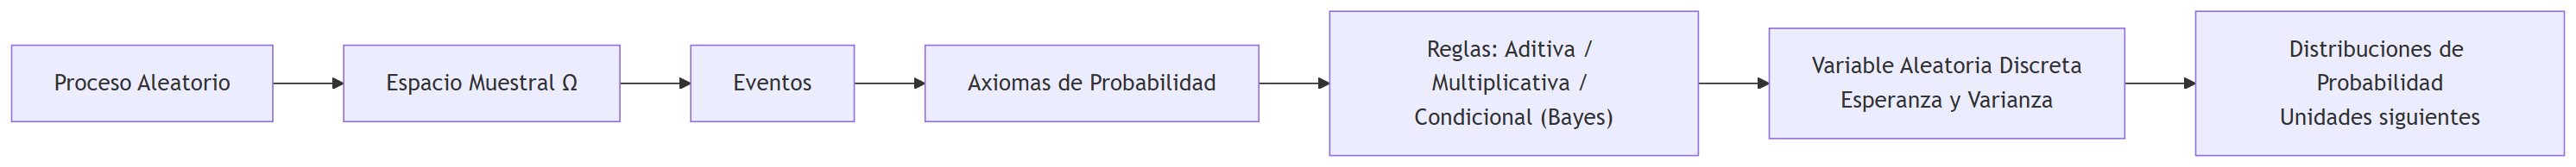
\includegraphics[width=18.92in,height=1.23in]{05_probabilidad_files/figure-latex/mermaid-figure-1.png}

Marco conceptual de la Unidad de Probabilidad

\section{Micro-ejercicios de aplicación
(optativos)}\label{micro-ejercicios-de-aplicaciuxf3n-optativos-2}

Los siguientes micro-ejercicios te permitirán practicar los conceptos
revisados en esta unidad. Puedes copiar y pegar las preguntas en un
script de R local, o bien utilizar \texttt{webR}, que es la versión
\emph{online} de R, disponible en esta guía.

\texttt{Nota}: los ejercicios están inspirados en trabajos científicos
publicados, pero contienen datos simulados. Por lo tanto, los resultados
obtenidos deben interpretarse únicamente con fines didácticos y no como
evidencia científica.

La finalidad es familiarizarse con el análisis estadístico y con el uso
de R a partir de situaciones similares a las que pueden encontrarse en
investigaciones reales.

\begin{Shaded}
\begin{Highlighting}[]


\CommentTok{\# =============================================================================}
\CommentTok{\# MICRO{-}EJERCICIOS OPTATIVOS — Probabilidad}
\CommentTok{\# =============================================================================}

\CommentTok{\# {-}{-}{-}{-}{-}{-}{-}{-}{-}{-}{-}{-}{-}{-}{-}{-}{-}{-}{-}{-}{-}{-}{-}{-}{-}{-}{-}{-}{-}{-}{-}{-}{-}{-}{-}{-}{-}{-}{-}{-}{-}{-}{-}{-}{-}{-}{-}{-}{-}{-}{-}{-}{-}{-}{-}{-}{-}{-}{-}{-}{-}{-}{-}{-}{-}{-}{-}{-}{-}{-}{-}{-}{-}{-}{-}{-}{-}}
\CommentTok{\# I. EXPERIMENTO ALEATORIO, ESPACIO MUESTRAL Y EVENTOS}
\CommentTok{\# {-}{-}{-}{-}{-}{-}{-}{-}{-}{-}{-}{-}{-}{-}{-}{-}{-}{-}{-}{-}{-}{-}{-}{-}{-}{-}{-}{-}{-}{-}{-}{-}{-}{-}{-}{-}{-}{-}{-}{-}{-}{-}{-}{-}{-}{-}{-}{-}{-}{-}{-}{-}{-}{-}{-}{-}{-}{-}{-}{-}{-}{-}{-}{-}{-}{-}{-}{-}{-}{-}{-}{-}{-}{-}{-}{-}{-}}

\CommentTok{\# 1) Contexto: En un relevamiento de fauna en la Reserva de Biosfera Laguna de}
\CommentTok{\#    Pozuelos, un observador selecciona al azar un grupo familiar de guanaco}
\CommentTok{\#    (Lama guanicoe) y registra si el macho dominante del grupo es territorial}
\CommentTok{\#    (T) o no (E).}
\CommentTok{\#    a) Identifique el experimento aleatorio.}
\CommentTok{\#    b) Escriba el espacio muestral Ω.}
\CommentTok{\#    c) ¿Cuántos puntos muestrales tiene Ω?}
\CommentTok{\#    Comente.}


\CommentTok{\# 2) Contexto: Se capturan 2 individuos de taruca (Hippocamelus antisensis) en}
\CommentTok{\#    un cerco de arreo en los Nevados de Cachi (límite Jujuy{-}Salta) y se}
\CommentTok{\#    registra el sexo de cada uno (Macho/Hembra), respetando el orden de}
\CommentTok{\#    captura.}
\CommentTok{\#    a) Escriba el espacio muestral Ω del experimento.}
\CommentTok{\#    b) ¿Cuántos puntos muestrales tiene Ω?}
\CommentTok{\#    c) Defina el evento A = "ambos individuos son hembras" y liste los}
\CommentTok{\#       puntos muestrales que lo componen.}
\CommentTok{\#    Comente si A es un evento simple o compuesto.}


\CommentTok{\# 3) Contexto: En un nido de ñandú de la Puna (Rhea pennata garleppi) se}
\CommentTok{\#    registra si cada uno de los 3 huevos incubados resulta viable (V) o no}
\CommentTok{\#    viable (N).}
\CommentTok{\#    a) Escriba el espacio muestral Ω.}
\CommentTok{\#    b) ¿Cuántos puntos muestrales lo componen?}
\CommentTok{\#    c) Defina el evento B = "exactamente dos huevos viables" y liste sus}
\CommentTok{\#       puntos muestrales.}
\CommentTok{\#    Comente.}


\CommentTok{\# 4) Contexto: Se define la variable G = "germinación de una semilla de}
\CommentTok{\#    queñoa (Polylepis australis) en un ensayo de vivero", con dos resultados}
\CommentTok{\#    posibles: germina (G) o no germina (NoG).}
\CommentTok{\#    a) Escriba el espacio muestral Ω.}
\CommentTok{\#    b) Clasifique a Ω según su cardinalidad (finito/infinito, numerable/no}
\CommentTok{\#       numerable).}
\CommentTok{\#    Comente, comparando con el ejemplo de germinación de maíz capia visto en}
\CommentTok{\#    la guía de cátedra.}


\CommentTok{\# 5) Contexto: En un punto de conteo de aves en las Yungas de Jujuy, un}
\CommentTok{\#    ornitólogo registra el número de individuos de parina grande}
\CommentTok{\#    (Phoenicoparrus andinus) avistados en una bandada, sin un máximo teórico}
\CommentTok{\#    acotado de antemano.}
\CommentTok{\#    a) Escriba el espacio muestral Ω.}
\CommentTok{\#    b) Clasifique a Ω según su cardinalidad.}
\CommentTok{\#    Comente por qué, en la práctica, se trunca el conteo a un valor máximo}
\CommentTok{\#    razonable.}


\CommentTok{\# {-}{-}{-}{-}{-}{-}{-}{-}{-}{-}{-}{-}{-}{-}{-}{-}{-}{-}{-}{-}{-}{-}{-}{-}{-}{-}{-}{-}{-}{-}{-}{-}{-}{-}{-}{-}{-}{-}{-}{-}{-}{-}{-}{-}{-}{-}{-}{-}{-}{-}{-}{-}{-}{-}{-}{-}{-}{-}{-}{-}{-}{-}{-}{-}{-}{-}{-}{-}{-}{-}{-}{-}{-}{-}{-}{-}{-}}
\CommentTok{\# II. PROBABILIDAD CLÁSICA Y FRECUENTISTA}
\CommentTok{\# {-}{-}{-}{-}{-}{-}{-}{-}{-}{-}{-}{-}{-}{-}{-}{-}{-}{-}{-}{-}{-}{-}{-}{-}{-}{-}{-}{-}{-}{-}{-}{-}{-}{-}{-}{-}{-}{-}{-}{-}{-}{-}{-}{-}{-}{-}{-}{-}{-}{-}{-}{-}{-}{-}{-}{-}{-}{-}{-}{-}{-}{-}{-}{-}{-}{-}{-}{-}{-}{-}{-}{-}{-}{-}{-}{-}{-}}

\CommentTok{\# 6) Contexto: En un estudio de estructura poblacional de vizcacha de la}
\CommentTok{\#    sierra (Lagidium viscacia) en afloramientos rocosos de la Puna, se}
\CommentTok{\#    examinan 150 individuos y se registra su sexo y la presencia de}
\CommentTok{\#    ectoparásitos.}
\CommentTok{\#}
\CommentTok{\#    Matriz de frecuencias observadas (Sexo vs Parasitismo):}
\CommentTok{\#    Filas: Hembra (H), Macho (M)}
\CommentTok{\#    Columnas: Parasitado (P), No parasitado (NP)}

\NormalTok{vizcachas }\OtherTok{=} \FunctionTok{matrix}\NormalTok{(}\FunctionTok{c}\NormalTok{(}\DecValTok{38}\NormalTok{, }\DecValTok{52}\NormalTok{, }\DecValTok{27}\NormalTok{, }\DecValTok{33}\NormalTok{), }\AttributeTok{nrow =} \DecValTok{2}\NormalTok{, }\AttributeTok{byrow =} \ConstantTok{TRUE}\NormalTok{)}
\FunctionTok{rownames}\NormalTok{(vizcachas) }\OtherTok{=} \FunctionTok{c}\NormalTok{(}\StringTok{"Hembra"}\NormalTok{, }\StringTok{"Macho"}\NormalTok{)}
\FunctionTok{colnames}\NormalTok{(vizcachas) }\OtherTok{=} \FunctionTok{c}\NormalTok{(}\StringTok{"Parasitado"}\NormalTok{, }\StringTok{"No\_parasitado"}\NormalTok{)}

\CommentTok{\#    a) Calcule el total de individuos (N) y las frecuencias marginales}
\CommentTok{\#       (addmargins()).}
\CommentTok{\#    b) Calcule P(Hembra), P(Parasitado) y P(Hembra y Parasitado).}
\CommentTok{\#    c) Interprete}
\CommentTok{\# Su código aquí:}


\CommentTok{\# 7) Contexto: En un chaku (esquila comunitaria) de vicuñas (Vicugna vicugna)}
\CommentTok{\#    en la Puna jujeña se capturan 90 individuos, de los cuales 63 son}
\CommentTok{\#    adultos y el resto juveniles.}

\NormalTok{n\_vicunas }\OtherTok{=} \DecValTok{90}
\NormalTok{adultos\_vicuna }\OtherTok{=} \DecValTok{63}

\CommentTok{\#    a) Defina el evento E = "individuo adulto" y calcule su probabilidad}
\CommentTok{\#       frecuentista P(E).}
\CommentTok{\#    b) Interprete el resultado en términos de la estructura etaria de la}
\CommentTok{\#       población muestreada.}
\CommentTok{\# Su código aquí:}


\CommentTok{\# 8) Contexto: En un muestreo de artrópodos edáficos en un sector de Yungas}
\CommentTok{\#    degradado por incendios, se registran 120 individuos pertenecientes a 5}
\CommentTok{\#    especies.}
\CommentTok{\#}
\CommentTok{\#    Especie       Abundancia}
\CommentTok{\#    Especie A          50}
\CommentTok{\#    Especie B          28}
\CommentTok{\#    Especie C          20}
\CommentTok{\#    Especie D          14}
\CommentTok{\#    Especie E           8}

\NormalTok{abundancias\_artropodos }\OtherTok{=} \FunctionTok{c}\NormalTok{(}\DecValTok{50}\NormalTok{, }\DecValTok{28}\NormalTok{, }\DecValTok{20}\NormalTok{, }\DecValTok{14}\NormalTok{, }\DecValTok{8}\NormalTok{)}

\CommentTok{\#    a) Calcule el Índice de Simpson (D).}
\CommentTok{\#    b) Calcule el Índice de Diversidad (1 {-} D) e interprete en términos probabilísticos.}
\CommentTok{\# Su código aquí:}


\CommentTok{\# 9) Contexto: En una parcela de regeneración natural de algarrobo negro}
\CommentTok{\#    (Prosopis nigra) en el Chaco jujeño se relevaron 85 plantines de un año,}
\CommentTok{\#    de los cuales 61 sobrevivieron a la primera estación seca.}

\NormalTok{n\_plantines\_algarrobo }\OtherTok{=} \DecValTok{85}
\NormalTok{sobrevivientes\_algarrobo }\OtherTok{=} \DecValTok{61}

\CommentTok{\#    a) Defina el evento S = "plantín sobrevive a la primera estación seca" y}
\CommentTok{\#       calcule P(S).}
\CommentTok{\#    b) Calcule la probabilidad complementaria P(Sᶜ) e interprete en términos}
\CommentTok{\#       de manejo de la regeneración.}
\CommentTok{\# Su código aquí:}


\CommentTok{\# 10) Contexto: En un relicto de bosque de Yungas se identifican 4 tipos de}
\CommentTok{\#     sustrato de nidificación utilizados por el pato de torrentes}
\CommentTok{\#     (Merganetta armata): oquedad en roca, vegetación ribereña, barranco de}
\CommentTok{\#     tierra y raíces expuestas, considerados igualmente probables a priori}
\CommentTok{\#     por el investigador.}
\CommentTok{\#     a) Escriba el espacio muestral y asigne la probabilidad clásica a cada}
\CommentTok{\#        punto muestral.}
\CommentTok{\#     b) Calcule la probabilidad de que un nido se ubique en un sustrato}
\CommentTok{\#        vegetal (vegetación ribereña o raíces expuestas).}
\CommentTok{\#     Comente si el supuesto de equiprobabilidad es razonable en un estudio}
\CommentTok{\#     real de campo.}


\CommentTok{\# {-}{-}{-}{-}{-}{-}{-}{-}{-}{-}{-}{-}{-}{-}{-}{-}{-}{-}{-}{-}{-}{-}{-}{-}{-}{-}{-}{-}{-}{-}{-}{-}{-}{-}{-}{-}{-}{-}{-}{-}{-}{-}{-}{-}{-}{-}{-}{-}{-}{-}{-}{-}{-}{-}{-}{-}{-}{-}{-}{-}{-}{-}{-}{-}{-}{-}{-}{-}{-}{-}{-}{-}{-}{-}{-}{-}{-}}
\CommentTok{\# III. REGLA ADITIVA, EVENTOS SOLAPADOS Y MUTUAMENTE EXCLUYENTES}
\CommentTok{\# {-}{-}{-}{-}{-}{-}{-}{-}{-}{-}{-}{-}{-}{-}{-}{-}{-}{-}{-}{-}{-}{-}{-}{-}{-}{-}{-}{-}{-}{-}{-}{-}{-}{-}{-}{-}{-}{-}{-}{-}{-}{-}{-}{-}{-}{-}{-}{-}{-}{-}{-}{-}{-}{-}{-}{-}{-}{-}{-}{-}{-}{-}{-}{-}{-}{-}{-}{-}{-}{-}{-}{-}{-}{-}{-}{-}{-}}

\CommentTok{\# 11) Contexto: En un relevamiento herpetológico en los Valles Templados de}
\CommentTok{\#     Jujuy se evalúan 130 transectas para registrar la presencia de dos}
\CommentTok{\#     especies de lagartija del género Liolaemus: L. irregularis (Evento A,}
\CommentTok{\#     presente en 48 transectas) y L. quilmes (Evento B, presente en 35}
\CommentTok{\#     transectas). En 14 transectas se registró la coexistencia de ambas}
\CommentTok{\#     especies.}

\NormalTok{n\_transectas\_liolaemus }\OtherTok{=} \DecValTok{130}
\NormalTok{nA\_liolaemus }\OtherTok{=} \DecValTok{48}\NormalTok{; nB\_liolaemus }\OtherTok{=} \DecValTok{35}\NormalTok{; nAB\_liolaemus }\OtherTok{=} \DecValTok{14}

\CommentTok{\#     a) Calcule P(A), P(B) y P(A ∩ B).}
\CommentTok{\#     b) ¿Los eventos A y B son mutuamente excluyentes? Aplique la regla}
\CommentTok{\#        aditiva correspondiente para calcular P(A ∪ B).}
\CommentTok{\#     c) Calcule la probabilidad de que en una transecta no se registre}
\CommentTok{\#        ninguna de las dos especies.}
\CommentTok{\# Su código aquí:}


\CommentTok{\# 12) Contexto: En un ensayo de sanidad vegetal sobre 90 plantines de quinoa}
\CommentTok{\#     (Chenopodium quinoa) inoculados con Trichoderma spp., se registra la}
\CommentTok{\#     presencia de dos problemas fitosanitarios: mildiu (Evento M, en 22}
\CommentTok{\#     plantines) y pudrición radicular (Evento R, en 15 plantines), con 6}
\CommentTok{\#     plantines afectados por ambos problemas simultáneamente.}

\NormalTok{n\_plantines\_quinoa }\OtherTok{=} \DecValTok{90}
\NormalTok{nM\_quinoa }\OtherTok{=} \DecValTok{22}\NormalTok{; nR\_quinoa }\OtherTok{=} \DecValTok{15}\NormalTok{; nMR\_quinoa }\OtherTok{=} \DecValTok{6}

\CommentTok{\#     a) Calcule P(M), P(R) y P(M ∩ R).}
\CommentTok{\#     b) Calcule la probabilidad de que un plantín presente al menos uno de}
\CommentTok{\#        los dos problemas.}
\CommentTok{\#     c) Calcule la probabilidad de que un plantín esté completamente sano.}
\CommentTok{\# Su código aquí:}


\CommentTok{\# 13) Contexto: En un muestreo de calidad de agua en 40 vertientes de la}
\CommentTok{\#     Quebrada de Humahuaca se clasifica cada vertiente según supere (Evento}
\CommentTok{\#     X) o no el límite de arsénico, y según supere (Evento Y) o no el}
\CommentTok{\#     límite de boro. Se sabe que P(X) = 0.30, P(Y) = 0.25 y P(X ∩ Y) = 0.10.}

\NormalTok{p\_X\_arsenico }\OtherTok{=} \FloatTok{0.30}
\NormalTok{p\_Y\_boro }\OtherTok{=} \FloatTok{0.25}
\NormalTok{p\_XY\_arsenico\_boro }\OtherTok{=} \FloatTok{0.10}

\CommentTok{\#     a) Calcule P(X ∪ Y): probabilidad de que una vertiente supere al menos}
\CommentTok{\#        uno de los dos límites.}
\CommentTok{\#     b) Calcule la probabilidad de que una vertiente sea apta según ambos}
\CommentTok{\#        parámetros simultáneamente.}
\CommentTok{\# Su código aquí:}


\CommentTok{\# 14) Contexto: Se clasifica la cobertura vegetal dominante en 60 sitios de}
\CommentTok{\#     muestreo de la Puna jujeña en tres categorías mutuamente excluyentes:}
\CommentTok{\#     Pastizal (24 sitios), Bofedal (16 sitios) y Roquedal (20 sitios).}

\NormalTok{cobertura\_puna }\OtherTok{=} \FunctionTok{c}\NormalTok{(}\AttributeTok{Pastizal =} \DecValTok{24}\NormalTok{, }\AttributeTok{Bofedal =} \DecValTok{16}\NormalTok{, }\AttributeTok{Roquedal =} \DecValTok{20}\NormalTok{)}

\CommentTok{\#     a) Verifique que las tres categorías son mutuamente excluyentes y}
\CommentTok{\#        exhaustivas.}
\CommentTok{\#     b) Calcule la probabilidad de que un sitio sea Pastizal o Bofedal.}
\CommentTok{\# Su código aquí:}


\CommentTok{\# 15) Contexto: En un estudio de conservación de humedales altoandinos se}
\CommentTok{\#     evalúa la presencia de tres especies de aves acuáticas en 100}
\CommentTok{\#     bofedales: flamenco austral (30 bofedales), parina chica (25}
\CommentTok{\#     bofedales) y pato puna (20 bofedales), sabiendo que ningún bofedal}
\CommentTok{\#     registró más de una especie en el muestreo (categorías mutuamente}
\CommentTok{\#     excluyentes por diseño).}

\NormalTok{n\_bofedales\_aves }\OtherTok{=} \DecValTok{100}
\NormalTok{flamenco\_austral }\OtherTok{=} \DecValTok{30}\NormalTok{; parina\_chica }\OtherTok{=} \DecValTok{25}\NormalTok{; pato\_puna }\OtherTok{=} \DecValTok{20}

\CommentTok{\#     a) Calcule la probabilidad de que un bofedal seleccionado al azar}
\CommentTok{\#        tenga alguna de las tres especies.}
\CommentTok{\#     b) Calcule la probabilidad de que no se registre ninguna de las tres}
\CommentTok{\#        especies.}
\CommentTok{\# Su código aquí:}


\CommentTok{\# {-}{-}{-}{-}{-}{-}{-}{-}{-}{-}{-}{-}{-}{-}{-}{-}{-}{-}{-}{-}{-}{-}{-}{-}{-}{-}{-}{-}{-}{-}{-}{-}{-}{-}{-}{-}{-}{-}{-}{-}{-}{-}{-}{-}{-}{-}{-}{-}{-}{-}{-}{-}{-}{-}{-}{-}{-}{-}{-}{-}{-}{-}{-}{-}{-}{-}{-}{-}{-}{-}{-}{-}{-}{-}{-}{-}{-}}
\CommentTok{\# IV. INDEPENDENCIA DE EVENTOS}
\CommentTok{\# {-}{-}{-}{-}{-}{-}{-}{-}{-}{-}{-}{-}{-}{-}{-}{-}{-}{-}{-}{-}{-}{-}{-}{-}{-}{-}{-}{-}{-}{-}{-}{-}{-}{-}{-}{-}{-}{-}{-}{-}{-}{-}{-}{-}{-}{-}{-}{-}{-}{-}{-}{-}{-}{-}{-}{-}{-}{-}{-}{-}{-}{-}{-}{-}{-}{-}{-}{-}{-}{-}{-}{-}{-}{-}{-}{-}{-}}

\CommentTok{\# 16) Retome la matriz de vizcachas del ejercicio 6 (sexo vs. parasitismo).}
\CommentTok{\#     a) Determine si el sexo del individuo y la presencia de ectoparásitos}
\CommentTok{\#        son eventos independientes.}
\CommentTok{\#     b) Interprete el resultado en términos de la dinámica de transmisión}
\CommentTok{\#        de parásitos en la población.}
\CommentTok{\# Su código aquí:}


\CommentTok{\# 17) Contexto: En 200 parcelas de bosque chaqueño se registra si cada}
\CommentTok{\#     parcela fue afectada por un incendio en los últimos 5 años (Evento F,}
\CommentTok{\#     70 parcelas) y si presenta regeneración de quebracho blanco}
\CommentTok{\#     (Aspidosperma quebracho{-}blanco) (Evento R, 90 parcelas). De las}
\CommentTok{\#     parcelas quemadas, 28 presentan regeneración.}

\NormalTok{n\_parcelas\_chaco }\OtherTok{=} \DecValTok{200}
\NormalTok{nF\_incendio }\OtherTok{=} \DecValTok{70}\NormalTok{; nR\_regeneracion }\OtherTok{=} \DecValTok{90}\NormalTok{; nFR\_incendio\_regen }\OtherTok{=} \DecValTok{28}

\CommentTok{\#     a) Calcule P(F), P(R) y P(F ∩ R).}
\CommentTok{\#     b) Determine si los eventos F y R son independientes.}
\CommentTok{\#     c) Interprete el resultado en términos de la resiliencia post{-}fuego}
\CommentTok{\#        del quebracho blanco.}
\CommentTok{\# Su código aquí:}


\CommentTok{\# 18) Contexto: En un relevamiento genético de 180 individuos de bagre de}
\CommentTok{\#     torrente (Trichomycterus sp.) en dos afluentes del Río Grande de}
\CommentTok{\#     Jujuy, se registra el sitio de captura y la presencia de un morfotipo}
\CommentTok{\#     de coloración particular.}

\NormalTok{morfotipos\_bagre }\OtherTok{=} \FunctionTok{matrix}\NormalTok{(}\FunctionTok{c}\NormalTok{(}\DecValTok{42}\NormalTok{, }\DecValTok{48}\NormalTok{, }\DecValTok{38}\NormalTok{, }\DecValTok{52}\NormalTok{), }\AttributeTok{nrow =} \DecValTok{2}\NormalTok{, }\AttributeTok{byrow =} \ConstantTok{TRUE}\NormalTok{)}
\FunctionTok{rownames}\NormalTok{(morfotipos\_bagre) }\OtherTok{=} \FunctionTok{c}\NormalTok{(}\StringTok{"Afluente\_1"}\NormalTok{, }\StringTok{"Afluente\_2"}\NormalTok{)}
\FunctionTok{colnames}\NormalTok{(morfotipos\_bagre) }\OtherTok{=} \FunctionTok{c}\NormalTok{(}\StringTok{"Morfotipo\_presente"}\NormalTok{, }\StringTok{"Morfotipo\_ausente"}\NormalTok{)}

\CommentTok{\#     a) Calcule las probabilidades marginales y la probabilidad conjunta de}
\CommentTok{\#        "Afluente 1 y Morfotipo presente".}
\CommentTok{\#     b) Determine si el sitio de captura y la presencia del morfotipo son}
\CommentTok{\#        eventos independientes.}
\CommentTok{\#     c) Interprete en términos de flujo génico entre las subpoblaciones.}
\CommentTok{\# Su código aquí:}


\CommentTok{\# 19) Contexto: Un gen loci en una población de chinchilla silvestre}
\CommentTok{\#     (Chinchilla chinchilla) de la Puna presenta dos alelos (A1, A2) con}
\CommentTok{\#     frecuencias p = 0.65 y q = 0.35. Asumiendo equilibrio de}
\CommentTok{\#     Hardy{-}Weinberg y selección aleatoria e independiente de ambos}
\CommentTok{\#     gametos:}

\NormalTok{p\_A1\_chinchilla }\OtherTok{=} \FloatTok{0.65}
\NormalTok{p\_A2\_chinchilla }\OtherTok{=} \FloatTok{0.35}

\CommentTok{\#     a) Calcule la probabilidad de que un individuo sea homocigoto A1A1.}
\CommentTok{\#     b) Calcule la probabilidad de que un individuo sea heterocigoto A1A2.}
\CommentTok{\#     c) Verifique que la suma de las probabilidades de todos los genotipos}
\CommentTok{\#        posibles es igual a 1.}
\CommentTok{\# Su código aquí:}


\CommentTok{\# {-}{-}{-}{-}{-}{-}{-}{-}{-}{-}{-}{-}{-}{-}{-}{-}{-}{-}{-}{-}{-}{-}{-}{-}{-}{-}{-}{-}{-}{-}{-}{-}{-}{-}{-}{-}{-}{-}{-}{-}{-}{-}{-}{-}{-}{-}{-}{-}{-}{-}{-}{-}{-}{-}{-}{-}{-}{-}{-}{-}{-}{-}{-}{-}{-}{-}{-}{-}{-}{-}{-}{-}{-}{-}{-}{-}{-}}
\CommentTok{\# V. PROBABILIDAD CONDICIONAL Y TEOREMA DE BAYES}
\CommentTok{\# {-}{-}{-}{-}{-}{-}{-}{-}{-}{-}{-}{-}{-}{-}{-}{-}{-}{-}{-}{-}{-}{-}{-}{-}{-}{-}{-}{-}{-}{-}{-}{-}{-}{-}{-}{-}{-}{-}{-}{-}{-}{-}{-}{-}{-}{-}{-}{-}{-}{-}{-}{-}{-}{-}{-}{-}{-}{-}{-}{-}{-}{-}{-}{-}{-}{-}{-}{-}{-}{-}{-}{-}{-}{-}{-}{-}{-}}

\CommentTok{\# 20) Contexto: En un programa de vigilancia sanitaria de camélidos, se}
\CommentTok{\#     evalúa la presencia de sarna sarcóptica en tropas de llama (Lama}
\CommentTok{\#     glama) de la Puna mediante inspección visual de campo.}
\CommentTok{\#}
\CommentTok{\#     Situación:}
\CommentTok{\#     {-} Prevalencia estimada de sarna en la población: P(D) = 0.12.}
\CommentTok{\#     {-} Sensibilidad de la inspección visual: P(+|D) = 0.85.}
\CommentTok{\#     {-} Especificidad de la inspección visual: P({-}|Dᶜ) = 0.90.}

\NormalTok{p\_D\_sarna }\OtherTok{=} \FloatTok{0.12}
\NormalTok{p\_pos\_dado\_D\_sarna }\OtherTok{=} \FloatTok{0.85}
\NormalTok{p\_neg\_dado\_Dc\_sarna }\OtherTok{=} \FloatTok{0.90}

\CommentTok{\#     a) Calcule la probabilidad total de que un animal inspeccionado al}
\CommentTok{\#        azar dé resultado positivo P(+).}
\CommentTok{\#     b) Aplique el Teorema de Bayes para calcular el Valor Predictivo}
\CommentTok{\#        Positivo P(D|+).}
\CommentTok{\#     c) Interprete la utilidad de la inspección visual como herramienta de}
\CommentTok{\#        tamizaje en terreno.}
\CommentTok{\# Su código aquí:}


\CommentTok{\# 21) Contexto: En un peritaje biológico sobre decomiso de fauna silvestre,}
\CommentTok{\#     se realiza una prueba de identificación molecular para determinar si}
\CommentTok{\#     una muestra de pelo corresponde a Puma concolor o a un cánido}
\CommentTok{\#     doméstico.}
\CommentTok{\#}
\CommentTok{\#     Situación:}
\CommentTok{\#     {-} Probabilidad a priori de que la muestra sea de puma: P(Pu) = 0.20.}
\CommentTok{\#     {-} La prueba da positivo cuando la muestra es de puma: P(+|Pu) = 0.97.}
\CommentTok{\#     {-} La prueba da falso positivo en muestras de cánido: P(+|Puᶜ) = 0.04.}

\NormalTok{p\_Pu }\OtherTok{=} \FloatTok{0.20}
\NormalTok{p\_pos\_dado\_Pu }\OtherTok{=} \FloatTok{0.97}
\NormalTok{p\_pos\_dado\_Pucomp }\OtherTok{=} \FloatTok{0.04}

\CommentTok{\#     a) Calcule la probabilidad de que una muestra elegida al azar dé}
\CommentTok{\#        resultado positivo P(+).}
\CommentTok{\#     b) Calcule el Valor Predictivo Positivo P(Pu|+).}
\CommentTok{\#     c) Elabore una breve conclusión técnica sobre la confiabilidad de la}
\CommentTok{\#        prueba para un dictamen pericial.}
\CommentTok{\# Su código aquí:}


\CommentTok{\# 22) Contexto: En el monitoreo de calidad de agua de una cuenca minera de la}
\CommentTok{\#     Puna, se utiliza al anfípodo Hyalella sp. como bioindicador.}
\CommentTok{\#}
\CommentTok{\#     {-} La probabilidad de que un punto de muestreo supere el límite de}
\CommentTok{\#       plomo es P(Pb) = 0.18.}
\CommentTok{\#     {-} Si se supera el límite de plomo, la probabilidad de mortalidad}
\CommentTok{\#       significativa de Hyalella es P(M|Pb) = 0.75.}
\CommentTok{\#     {-} Si no se supera el límite, la probabilidad de mortalidad}
\CommentTok{\#       significativa es P(M|Pbᶜ) = 0.08.}

\NormalTok{p\_Pb }\OtherTok{=} \FloatTok{0.18}
\NormalTok{p\_M\_dado\_Pb }\OtherTok{=} \FloatTok{0.75}
\NormalTok{p\_M\_dado\_Pbcomp }\OtherTok{=} \FloatTok{0.08}

\CommentTok{\#     a) Calcule la probabilidad total de observar mortalidad significativa}
\CommentTok{\#        de Hyalella P(M).}
\CommentTok{\#     b) Si se observa mortalidad significativa en un punto, calcule la}
\CommentTok{\#        probabilidad de que dicho punto supere el límite de plomo P(Pb|M).}
\CommentTok{\#     c) Interprete la eficiencia de Hyalella sp. como bioindicador de}
\CommentTok{\#        contaminación por plomo.}
\CommentTok{\# Su código aquí:}


\CommentTok{\# 23) Contexto: Se caracterizaron 20 majadas caprinas de dos departamentos de}
\CommentTok{\#     la Puna jujeña (Susques y Rinconada) según su estado sanitario}
\CommentTok{\#     respecto a fasciolosis (Libre / No libre).}
\CommentTok{\#}
\CommentTok{\#     Tabla de contingencia (majadas):}
\CommentTok{\#                  Libre   No\_libre}
\CommentTok{\#     Susques        7         3}
\CommentTok{\#     Rinconada      5         5}

\NormalTok{fasciolosis }\OtherTok{=} \FunctionTok{matrix}\NormalTok{(}\FunctionTok{c}\NormalTok{(}\DecValTok{7}\NormalTok{, }\DecValTok{3}\NormalTok{, }\DecValTok{5}\NormalTok{, }\DecValTok{5}\NormalTok{), }\AttributeTok{nrow =} \DecValTok{2}\NormalTok{, }\AttributeTok{byrow =} \ConstantTok{TRUE}\NormalTok{)}
\FunctionTok{rownames}\NormalTok{(fasciolosis) }\OtherTok{=} \FunctionTok{c}\NormalTok{(}\StringTok{"Susques"}\NormalTok{, }\StringTok{"Rinconada"}\NormalTok{)}
\FunctionTok{colnames}\NormalTok{(fasciolosis) }\OtherTok{=} \FunctionTok{c}\NormalTok{(}\StringTok{"Libre"}\NormalTok{, }\StringTok{"No\_libre"}\NormalTok{)}

\CommentTok{\#     a) Calcule la probabilidad de que una majada esté libre de}
\CommentTok{\#        fasciolosis, sabiendo que es de Susques.}
\CommentTok{\#     b) Calcule la probabilidad de que una majada sea de Rinconada,}
\CommentTok{\#        sabiendo que está libre de fasciolosis.}
\CommentTok{\#     c) Compare ambos resultados con las probabilidades marginales}
\CommentTok{\#        correspondientes e interprete.}
\CommentTok{\# Su código aquí:}


\CommentTok{\# 24) Contexto: En una estación de monitoreo de fauna silvestre se}
\CommentTok{\#     identifican individuos de zorro colorado (Lycalopex culpaeus) mediante}
\CommentTok{\#     trampas cámara, clasificándolos como adultos o juveniles, y}
\CommentTok{\#     registrando además si presentan signos de sarna.}
\CommentTok{\#     {-} P(Adulto) = 0.70 ; P(Juvenil) = 0.30.}
\CommentTok{\#     {-} P(Sarna | Adulto) = 0.10 ; P(Sarna | Juvenil) = 0.25.}

\NormalTok{p\_adulto\_zorro }\OtherTok{=} \FloatTok{0.70}\NormalTok{; p\_juvenil\_zorro }\OtherTok{=} \FloatTok{0.30}
\NormalTok{p\_sarna\_dado\_adulto }\OtherTok{=} \FloatTok{0.10}\NormalTok{; p\_sarna\_dado\_juvenil }\OtherTok{=} \FloatTok{0.25}

\CommentTok{\#     a) Aplique el teorema de la probabilidad total para calcular}
\CommentTok{\#        P(Sarna).}
\CommentTok{\#     b) Calcule P(Juvenil | Sarna) mediante el Teorema de Bayes.}
\CommentTok{\#     c) Interprete el resultado en términos de vulnerabilidad sanitaria}
\CommentTok{\#        por clase etaria.}
\CommentTok{\# Su código aquí:}


\CommentTok{\# 25) Contexto: Se evalúa el desempeño de una prueba serológica rápida para}
\CommentTok{\#     detectar Trypanosoma cruzi (agente del Mal de Chagas) en reservorios}
\CommentTok{\#     silvestres (Dasypus novemcinctus, quirquincho) capturados en el Chaco}
\CommentTok{\#     jujeño. Se sabe que P(D) = 0.08, P(+|D) = 0.93 y P(+|Dᶜ) = 0.06.}

\NormalTok{p\_D\_chagas }\OtherTok{=} \FloatTok{0.08}
\NormalTok{p\_pos\_dado\_D\_chagas }\OtherTok{=} \FloatTok{0.93}
\NormalTok{p\_pos\_dado\_Dcomp\_chagas }\OtherTok{=} \FloatTok{0.06}

\CommentTok{\#     a) Calcule P(+) y P(D|+).}
\CommentTok{\#     b) Calcule el Valor Predictivo Negativo P(Dᶜ|{-}).}
\CommentTok{\#     c) Discuta la utilidad de la prueba para el monitoreo epidemiológico}
\CommentTok{\#        de reservorios silvestres.}
\CommentTok{\# Su código aquí:}


\CommentTok{\# {-}{-}{-}{-}{-}{-}{-}{-}{-}{-}{-}{-}{-}{-}{-}{-}{-}{-}{-}{-}{-}{-}{-}{-}{-}{-}{-}{-}{-}{-}{-}{-}{-}{-}{-}{-}{-}{-}{-}{-}{-}{-}{-}{-}{-}{-}{-}{-}{-}{-}{-}{-}{-}{-}{-}{-}{-}{-}{-}{-}{-}{-}{-}{-}{-}{-}{-}{-}{-}{-}{-}{-}{-}{-}{-}{-}{-}}
\CommentTok{\# VI. VARIABLES ALEATORIAS DISCRETAS — FUNCIÓN DE PROBABILIDAD, ESPERANZA Y VARIANZA}
\CommentTok{\# {-}{-}{-}{-}{-}{-}{-}{-}{-}{-}{-}{-}{-}{-}{-}{-}{-}{-}{-}{-}{-}{-}{-}{-}{-}{-}{-}{-}{-}{-}{-}{-}{-}{-}{-}{-}{-}{-}{-}{-}{-}{-}{-}{-}{-}{-}{-}{-}{-}{-}{-}{-}{-}{-}{-}{-}{-}{-}{-}{-}{-}{-}{-}{-}{-}{-}{-}{-}{-}{-}{-}{-}{-}{-}{-}{-}{-}}

\CommentTok{\# 26) Contexto: En un programa de conservación del cóndor andino (Vultur}
\CommentTok{\#     gryphus) en la Quebrada de Humahuaca, se define la variable aleatoria}
\CommentTok{\#     X: "número de pichones eclosionados por pareja reproductora en una}
\CommentTok{\#     temporada", con la siguiente función de probabilidad estimada a partir}
\CommentTok{\#     de 80 parejas monitoreadas:}

\NormalTok{x\_condor }\OtherTok{=} \FunctionTok{c}\NormalTok{(}\DecValTok{0}\NormalTok{, }\DecValTok{1}\NormalTok{)}
\NormalTok{prob\_condor }\OtherTok{=} \FunctionTok{c}\NormalTok{(}\FloatTok{0.35}\NormalTok{, }\FloatTok{0.65}\NormalTok{)}

\CommentTok{\#     a) Verifique que p(x) cumple los axiomas de una función de}
\CommentTok{\#        probabilidad.}
\CommentTok{\#     b) Calcule la Esperanza E(X) e interprete en términos de éxito}
\CommentTok{\#        reproductivo.}
\CommentTok{\#     c) Calcule la Varianza Var(X) y el desvío estándar.}
\CommentTok{\# Su código aquí:}


\CommentTok{\# 28) Contexto: En un estudio de comportamiento reproductivo del picaflor}
\CommentTok{\#     puneño (Oreotrochilus estella), se define X: "número de huevos por}
\CommentTok{\#     puesta", con la siguiente función de probabilidad observada a partir}
\CommentTok{\#     de 60 nidos:}

\NormalTok{x\_picaflor }\OtherTok{=} \FunctionTok{c}\NormalTok{(}\DecValTok{1}\NormalTok{, }\DecValTok{2}\NormalTok{, }\DecValTok{3}\NormalTok{)}
\NormalTok{prob\_picaflor }\OtherTok{=} \FunctionTok{c}\NormalTok{(}\FloatTok{0.15}\NormalTok{, }\FloatTok{0.70}\NormalTok{, }\FloatTok{0.15}\NormalTok{)}

\CommentTok{\#     a) Verifique los axiomas de probabilidad.}
\CommentTok{\#     b) Calcule F(x) mediante suma acumulada (cumsum()).}
\CommentTok{\#     c) Calcule E(X) y Var(X), e interprete el tamaño de puesta esperado.}
\CommentTok{\# Su código aquí:}


\CommentTok{\# 29) Contexto: En 40 trampas Sherman instaladas en un transecto de}
\CommentTok{\#     micromamíferos de las Yungas jujeñas, se registró el número de}
\CommentTok{\#     capturas por trampa durante una noche de muestreo, obteniéndose la}
\CommentTok{\#     siguiente distribución de frecuencias relativas, interpretada como una}
\CommentTok{\#     aproximación de la función de probabilidad de X: "número de capturas}
\CommentTok{\#     por trampa":}

\NormalTok{x\_capturas }\OtherTok{=} \FunctionTok{c}\NormalTok{(}\DecValTok{0}\NormalTok{, }\DecValTok{1}\NormalTok{, }\DecValTok{2}\NormalTok{, }\DecValTok{3}\NormalTok{)}
\NormalTok{prob\_capturas }\OtherTok{=} \FunctionTok{c}\NormalTok{(}\FloatTok{0.50}\NormalTok{, }\FloatTok{0.30}\NormalTok{, }\FloatTok{0.15}\NormalTok{, }\FloatTok{0.05}\NormalTok{)}

\CommentTok{\#     a) Verifique los axiomas de probabilidad.}
\CommentTok{\#     b) Calcule E(X) y Var(X).}
\CommentTok{\#     c) Calcule la probabilidad acumulada de registrar como máximo 1}
\CommentTok{\#        captura P(X ≤ 1).}
\CommentTok{\#     d) Construya el gráfico de bastones de la función de probabilidad}
\CommentTok{\#        (barplot()).}
\CommentTok{\# Su código aquí:}


\CommentTok{\# 30) Contexto integrador: En un bofedal de la Puna jujeña se realiza el}
\CommentTok{\#     monitoreo de sapo andino (Rhinella spinulosa). Se sabe que la}
\CommentTok{\#     probabilidad de que un bofedal presente contaminación por}
\CommentTok{\#     agroquímicos es P(C) = 0.20. En bofedales contaminados, el número de}
\CommentTok{\#     individuos de sapo observados por transecta (X) sigue la función de}
\CommentTok{\#     probabilidad:}

\NormalTok{x\_sapo\_contaminado }\OtherTok{=} \FunctionTok{c}\NormalTok{(}\DecValTok{0}\NormalTok{, }\DecValTok{1}\NormalTok{, }\DecValTok{2}\NormalTok{)}
\NormalTok{prob\_sapo\_contaminado }\OtherTok{=} \FunctionTok{c}\NormalTok{(}\FloatTok{0.60}\NormalTok{, }\FloatTok{0.30}\NormalTok{, }\FloatTok{0.10}\NormalTok{)}

\CommentTok{\#     mientras que en bofedales no contaminados:}

\NormalTok{x\_sapo\_sano }\OtherTok{=} \FunctionTok{c}\NormalTok{(}\DecValTok{0}\NormalTok{, }\DecValTok{1}\NormalTok{, }\DecValTok{2}\NormalTok{, }\DecValTok{3}\NormalTok{, }\DecValTok{4}\NormalTok{)}
\NormalTok{prob\_sapo\_sano }\OtherTok{=} \FunctionTok{c}\NormalTok{(}\FloatTok{0.05}\NormalTok{, }\FloatTok{0.15}\NormalTok{, }\FloatTok{0.30}\NormalTok{, }\FloatTok{0.30}\NormalTok{, }\FloatTok{0.20}\NormalTok{)}

\CommentTok{\#     a) Calcule E(X) y Var(X) para cada escenario (contaminado / no}
\CommentTok{\#        contaminado).}
\CommentTok{\#     b) Compare ambos valores esperados e interprete el efecto de la}
\CommentTok{\#        contaminación sobre la abundancia de sapo andino.}
\CommentTok{\#     c) Si se selecciona una transecta al azar y se observan 0 individuos,}
\CommentTok{\#        y sabiendo además que P(X=0 | Cᶜ) = 0.05, aplique el Teorema de}
\CommentTok{\#        Bayes para calcular la probabilidad de que el bofedal esté}
\CommentTok{\#        contaminado dado ese resultado P(C | X=0).}
\CommentTok{\# Su código aquí:}

\CommentTok{\# =============================================================================}
\end{Highlighting}
\end{Shaded}

\bookmarksetup{startatroot}

\chapter*{\texorpdfstring{Mi primer cuaderno
\emph{Notebooklm}}{Mi primer cuaderno Notebooklm}}\label{mi-primer-cuaderno-notebooklm}
\addcontentsline{toc}{chapter}{Mi primer cuaderno \emph{Notebooklm}}

\markboth{Mi primer cuaderno \emph{Notebooklm}}{Mi primer cuaderno
\emph{Notebooklm}}

A partir del Trabajo Práctico 3 vamos a comenzar a realizar algunas
\emph{actividades de pre-clase o inter-clase}, utilizando el recurso
\texttt{Notebooklm} de Google. En clase comentaremos un poco más acerca
de las pautas de su empleo. En este apartado les compartimos un breve
instructivo de cómo crear un cuaderno y realizar configuraciones básicas
antes de comenzar a utilizarlo.

\section*{Primeros pasos}\label{primeros-pasos-1}
\addcontentsline{toc}{section}{Primeros pasos}

\markright{Primeros pasos}

A continuación se presenta un micro tutorial para que crear sus primeros
cuadernos en \emph{Notebooklm}, un entorno de aprendizaje basado en la
IA Gemini de Google.

\url{https://youtu.be/T4cqdV9f5vE?si=aQ3QO2WE0_t6G1-w&t=2}

Te recomendamos una lectura complementaria sobre la herramienta en este
\href{https://www.datacamp.com/es/tutorial/notebooklm}{enlace}.

Y por supuesto, complementa con la lectura de la Unidad 2 del libro
``Apuntes de Bioestadística. Con ejercicios resueltos'', acerca de
pautas de empleo de los cuadernos.

\begin{center}\rule{0.5\linewidth}{0.5pt}\end{center}

\bookmarksetup{startatroot}

\chapter{Trabajo Práctico 3: Distribuciones
Discretas}\label{trabajo-pruxe1ctico-3-distribuciones-discretas}

Objetivos del Trabajo Práctico El trabajo práctico tiene como objetivos:
(1) Reconocer situaciones donde los supuestos de los modelos Binomial y
Poisson resultan razonables (ensayos independientes con probabilidad
constante, o conteo de ocurrencias en un intervalo continuo de espacio o
tiempo); (2) Especificar correctamente los parámetros de cada
distribución a partir del contexto biológico o ambiental (n y p para el
modelo Binomial; λ para el modelo de Poisson); (3) Calcular e
interpretar probabilidades puntuales y acumuladas {[}P(X = k), P(X ≤ k),
P(X \textgreater{} k){]} utilizando las funciones de R correspondientes;
(4) Calcular e interpretar la esperanza, la varianza y el desvío
estándar de variables con distribución Binomial y de Poisson; (5)
Verificar las condiciones de aplicabilidad de la aproximación de la
distribución Binomial por la de Poisson, y aplicarla en el estudio de
eventos de baja probabilidad; y (6) Interpretar los resultados obtenidos
en el marco de la práctica profesional en Ciencias Biológicas.

\begin{tcolorbox}[enhanced jigsaw, arc=.35mm, bottomrule=.15mm, bottomtitle=1mm, breakable, colback=white, colbacktitle=quarto-callout-important-color!10!white, colframe=quarto-callout-important-color-frame, coltitle=black, left=2mm, leftrule=.75mm, opacityback=0, opacitybacktitle=0.6, rightrule=.15mm, title=\textcolor{quarto-callout-important-color}{\faExclamation}\hspace{0.5em}{Lectura Sugerida para el Trabajo Práctico}, titlerule=0mm, toprule=.15mm, toptitle=1mm]

Se recomienda a los estudiantes consultar el libro \textbf{«Apuntes de
Bioestadística. Con ejercicios resueltos»} para profundizar los
conceptos teóricos y metodológicos desarrollados en este marco:

\begin{itemize}
\tightlist
\item
  \textbf{Unidad 5: Distribución Binomial}: Consultar las condiciones de
  aplicabilidad del modelo (ensayos tipo Bernoulli, independencia,
  probabilidad de éxito constante), su definición formal y el cálculo de
  probabilidades puntuales y acumuladas.
\item
  \textbf{Unidad 5: Distribución de Poisson}: Revisar las condiciones
  del modelo (independencia de ocurrencias, tasa media constante λ,
  sucesos ``raros''), su definición formal y sus propiedades (esperanza
  y varianza iguales a λ).
\item
  \textbf{Unidad 5: Aproximación de la Binomial por la Poisson}: Prestar
  atención a las condiciones bajo las cuales dicha aproximación es
  válida, y a su utilidad práctica para el estudio de eventos de baja
  probabilidad en muestras grandes.
\end{itemize}

Como lecturas complementarias, se sugiere también revisar la unidad
\emph{«Modelos probabilísticos»} del libro \textbf{«Estadística y
Biometría»} de Balzarini et al., y la unidad \emph{«Statistical Models»}
del libro \textbf{«Data Analysis for the Life Sciences»} de Irizarry et
al.

\end{tcolorbox}

\section{Generalidades}\label{generalidades-1}

En la Unidad anterior se estableció que toda variable aleatoria discreta
queda caracterizada por una función de probabilidad de masa y su
correspondiente función de distribución acumulada. Ahora bien, en la
práctica no siempre es necesario construir esa función ``desde cero'':
existen modelos teóricos que, bajo determinados supuestos, permiten
asignar probabilidades a una variable discreta a partir de unos pocos
parámetros. En este Trabajo Práctico se trabaja con dos de los modelos
discretos más utilizados en Ciencias Biológicas: el modelo
\textbf{Binomial} y el modelo de \textbf{Poisson}.

\subsection{El modelo Binomial: conteo de éxitos en ensayos
independientes}\label{el-modelo-binomial-conteo-de-uxe9xitos-en-ensayos-independientes}

El modelo Binomial se aplica cuando un experimento consiste en repetir
un número fijo \emph{n} de ensayos independientes entre sí, cada uno con
solo dos resultados posibles (éxito/fracaso) y con una probabilidad de
éxito \emph{p} que se mantiene constante en cada ensayo. La variable de
interés es el número total de éxitos obtenidos, que puede tomar
cualquier valor entero entre 0 y \emph{n}. Este esquema aparece, por
ejemplo, al registrar cuántos individuos de una muestra presentan una
determinada condición (una infección, un fenotipo, la presencia de una
especie en un cuadrante), siempre que los individuos puedan considerarse
independientes entre sí y la probabilidad de la condición sea
razonablemente constante en la población muestreada.

\subsection{El modelo de Poisson: conteo de eventos en un
continuo}\label{el-modelo-de-poisson-conteo-de-eventos-en-un-continuo}

El modelo de Poisson, en cambio, no parte de un número fijo de ensayos,
sino de un intervalo continuo, por ejemplo de espacio o de tiempo, y
modela el número de veces que ocurre un evento dentro de ese intervalo.
Se aplica cuando los eventos ocurren de forma independiente unos de
otros, a una tasa media constante λ, y cuando la probabilidad de que
ocurra más de un evento en un intervalo infinitamente pequeño es
prácticamente nula. Es el modelo natural para conteos como el número de
individuos avistados por transecto, el número de larvas por cuadrante de
muestreo, o el número de lesiones por unidad de longitud de una
secuencia génica.

\subsection{De la Binomial a la Poisson: una aproximación
útil}\label{de-la-binomial-a-la-poisson-una-aproximaciuxf3n-uxfatil}

Cuando en un esquema Binomial el número de ensayos \emph{n} es muy
grande y la probabilidad de éxito \emph{p} es muy pequeña ---de modo que
su producto λ = n·p se mantiene moderado---, la distribución de Poisson
con parámetro λ constituye una buena aproximación de la distribución
Binomial. Esta propiedad resulta especialmente útil en Biología para
estudiar sucesos de baja probabilidad en muestras grandes, como la
aparición de una mutación rara en una población o el registro de una
especie poco frecuente en un muestreo extenso, evitando el cálculo
directo de factoriales con valores de \emph{n} muy grandes.

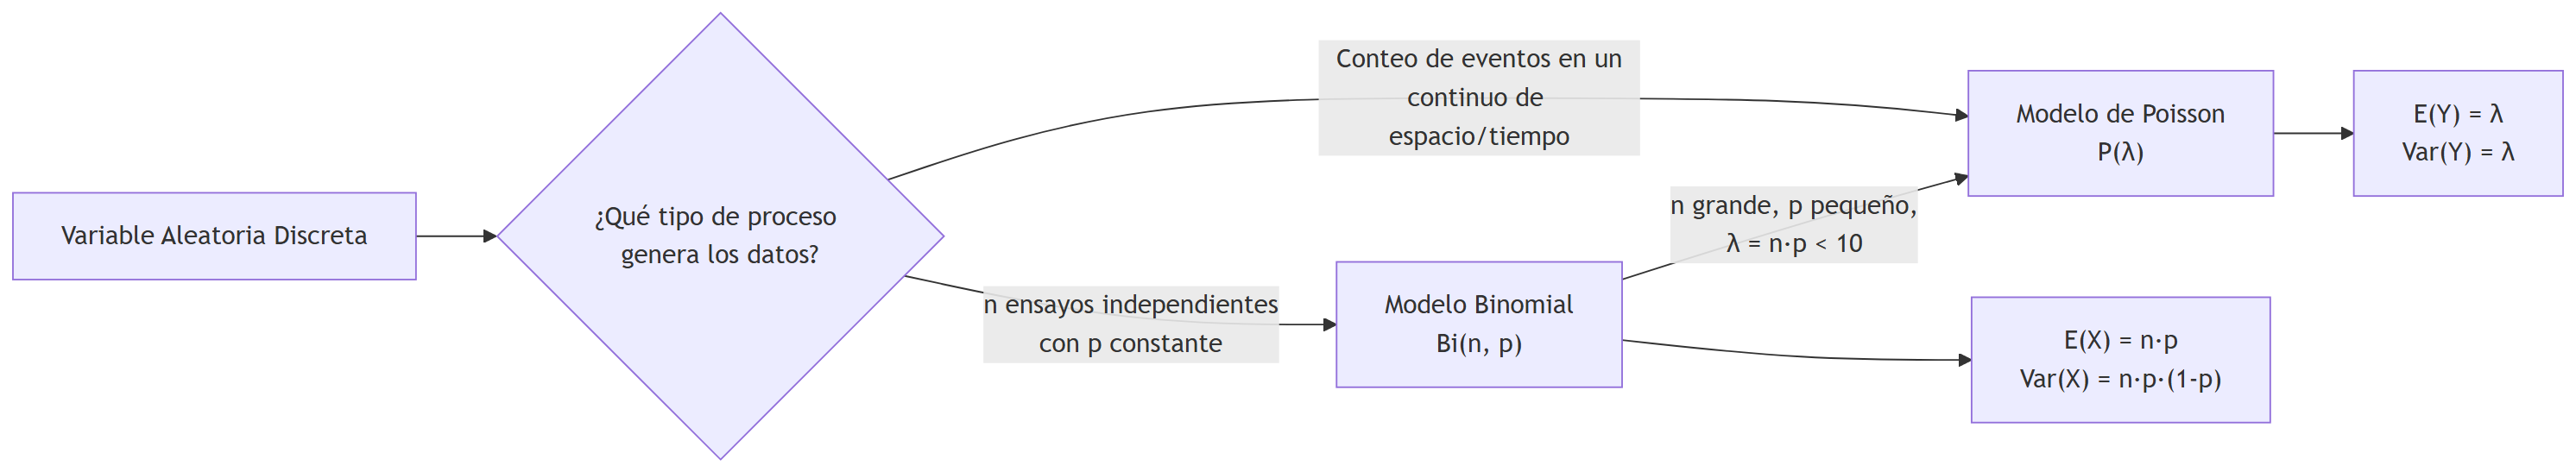
\includegraphics[width=16.69in,height=3.06in]{06_discretas_files/figure-latex/mermaid-figure-1.png}

Marco conceptual de la Unidad de Distribuciones Discretas

\section{\texorpdfstring{\textbf{Actividad de
pre-clase}}{Actividad de pre-clase}}\label{actividad-de-pre-clase}

Deberá copiar y pegar el siguiente \emph{prompt} dentro del chat del
cuaderno de \emph{Notebooklm} creado luego de la clase anterior. Luego
deberá copiar y pegar el ejercicio generado por la IA en un archivo .txt
o bien en un documento de word o similar.
\texttt{Se\ le\ solicitará\ la\ presentación\ del\ ejercicio\ durante\ la\ clase}.

\begin{Shaded}
\begin{Highlighting}[]

\NormalTok{Actúa como un docente de Bioestadística de la Licenciatura en Ciencias Biológicas. }
\NormalTok{Genera 1 único ejercicio basado en un caso de aplicación de estudio biológico que pueda ser resuelto utilizando las distribuciones Binomial y Poisson.}
\NormalTok{El ejercicio debe incluir incisos específicos para:}
\NormalTok{{-} Identificar la variable aleatoria y fundamentar los supuestos de ambos modelos.}
\NormalTok{{-} Definir los parámetros de cada distribución (n, p, lambda).}
\NormalTok{{-} Calcular la esperanza, varianza y desvío estándar para ambos modelos.}
\NormalTok{{-} Calcular probabilidades puntuales y acumuladas.}
\NormalTok{{-} Evaluar las condiciones de aplicabilidad de la aproximación de la Binomial por Poisson.}
\NormalTok{{-} Proporciona únicamente la consigna completa redactada de forma clara y directa. No generes la solución.}
\end{Highlighting}
\end{Shaded}

\section{\texorpdfstring{\textbf{Actividad de
clase}}{Actividad de clase}}\label{actividad-de-clase}

\textbf{Notas de clase}

\begin{itemize}
\tightlist
\item
  \textbf{Santiago, Paloma, Antonella} (Ejercicio 1)

  \begin{itemize}
  \tightlist
  \item
    \begin{enumerate}
    \def\labelenumi{\alph{enumi})}
    \tightlist
    \item
      Identificación correcta: Modelo Binomial con \texttt{n\ =\ 80},
      \texttt{p\ =\ 0,04}. \texttt{Nota:}faltó definir la variable
      aleatoria.
    \end{enumerate}
  \item
    \begin{enumerate}
    \def\labelenumi{\alph{enumi})}
    \setcounter{enumi}{1}
    \tightlist
    \item
      \texttt{P(X\ =\ 10)\ =\ 0,00099} (correcto).
    \end{enumerate}
  \item
    \begin{enumerate}
    \def\labelenumi{\alph{enumi})}
    \setcounter{enumi}{2}
    \tightlist
    \item
      \texttt{P(X\ ≥\ 5)\ =\ 0,2164} (correcto, precisión decimal
      adecuada).
    \end{enumerate}
  \item
    \begin{enumerate}
    \def\labelenumi{\alph{enumi})}
    \setcounter{enumi}{3}
    \tightlist
    \item
      \texttt{E(X)\ =\ 3,2}; \texttt{Var(X)\ =\ 3,072};
      \texttt{DE(X)\ =\ 1,7527} (correctos en su totalidad).
    \end{enumerate}
  \end{itemize}
\end{itemize}

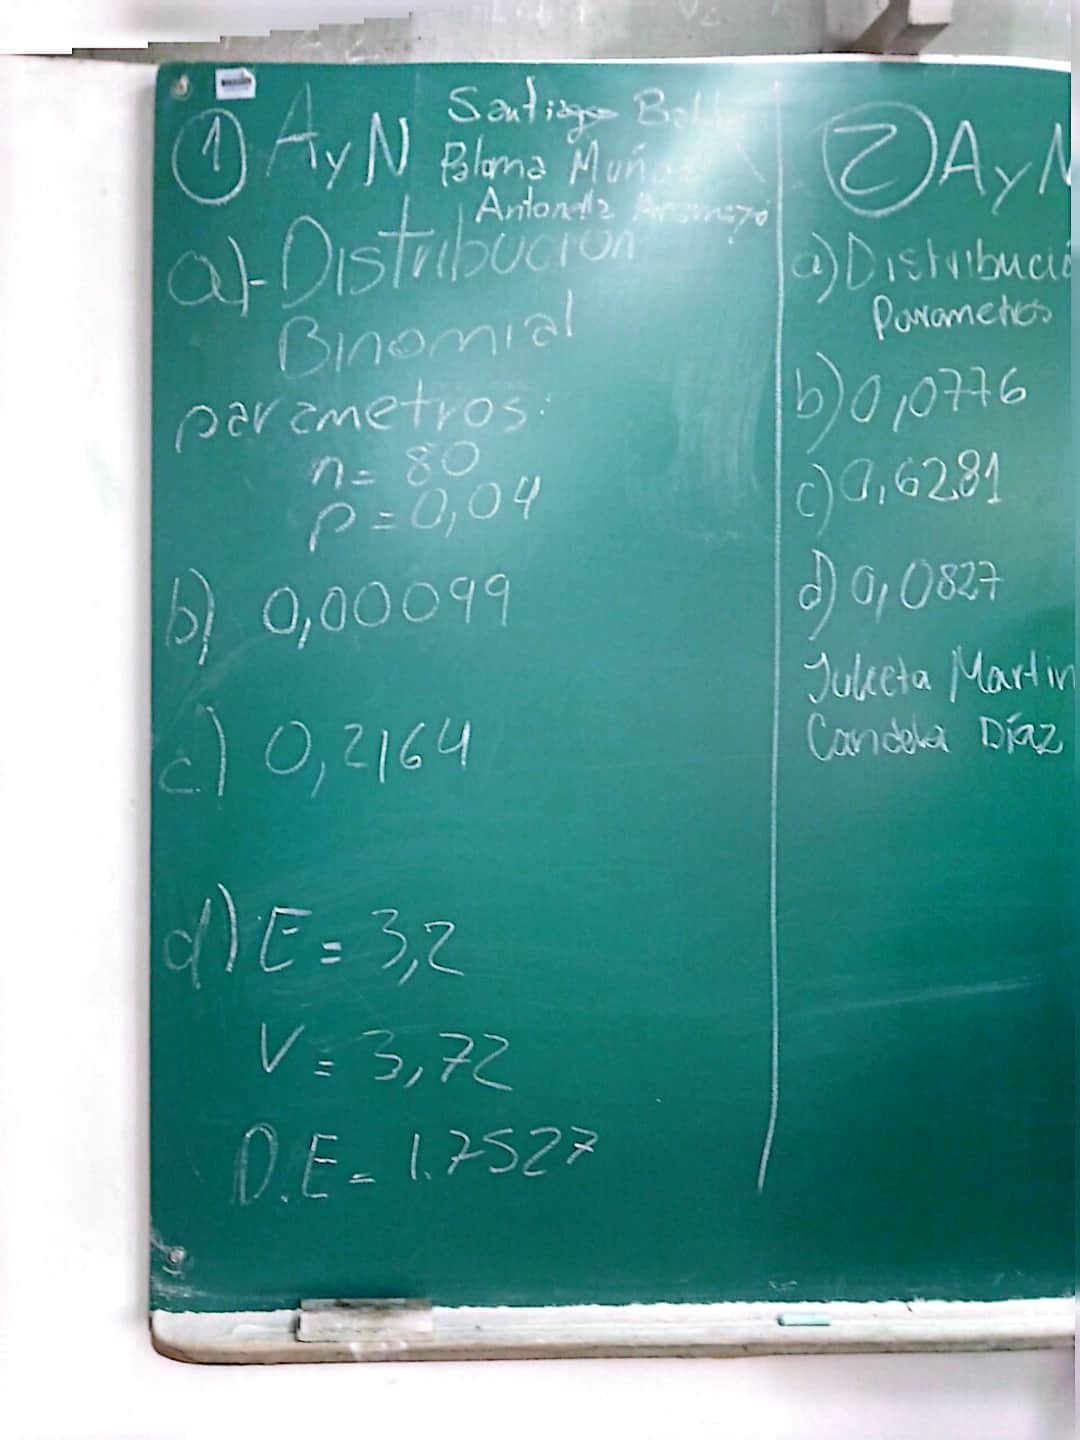
\includegraphics[width=0.4\linewidth,height=\textheight,keepaspectratio]{./IMAGENES/DISCRETAS/ej1-M.jpeg}

\begin{itemize}
\tightlist
\item
  \textbf{Arnaldo, Leandro, Kyara Avendaño, Veronica} (Ejercicio 3)

  \begin{itemize}
  \tightlist
  \item
    \begin{enumerate}
    \def\labelenumi{\alph{enumi})}
    \tightlist
    \item
      Identificación correcta: Modelo Binomial con \texttt{n\ =\ 80},
      \texttt{p\ =\ 0,04}.
    \end{enumerate}
  \item
    \begin{enumerate}
    \def\labelenumi{\alph{enumi})}
    \setcounter{enumi}{1}
    \tightlist
    \item
      \texttt{P(X\ =\ 10)\ =\ 0,00099} (correcto).
    \end{enumerate}
  \item
    \begin{enumerate}
    \def\labelenumi{\alph{enumi})}
    \setcounter{enumi}{2}
    \tightlist
    \item
      \texttt{P(X\ ≥\ 5)\ =\ 0,22} (correcto por redondeo).
    \end{enumerate}
  \item
    \begin{enumerate}
    \def\labelenumi{\alph{enumi})}
    \setcounter{enumi}{3}
    \tightlist
    \item
      \texttt{E(X)\ =\ 3,2} y \texttt{DE(X)\ =\ 1,75} (correctos).
      \textbf{Nota: Ustedes tenían que resolver el 3!}
    \end{enumerate}
  \end{itemize}
\end{itemize}

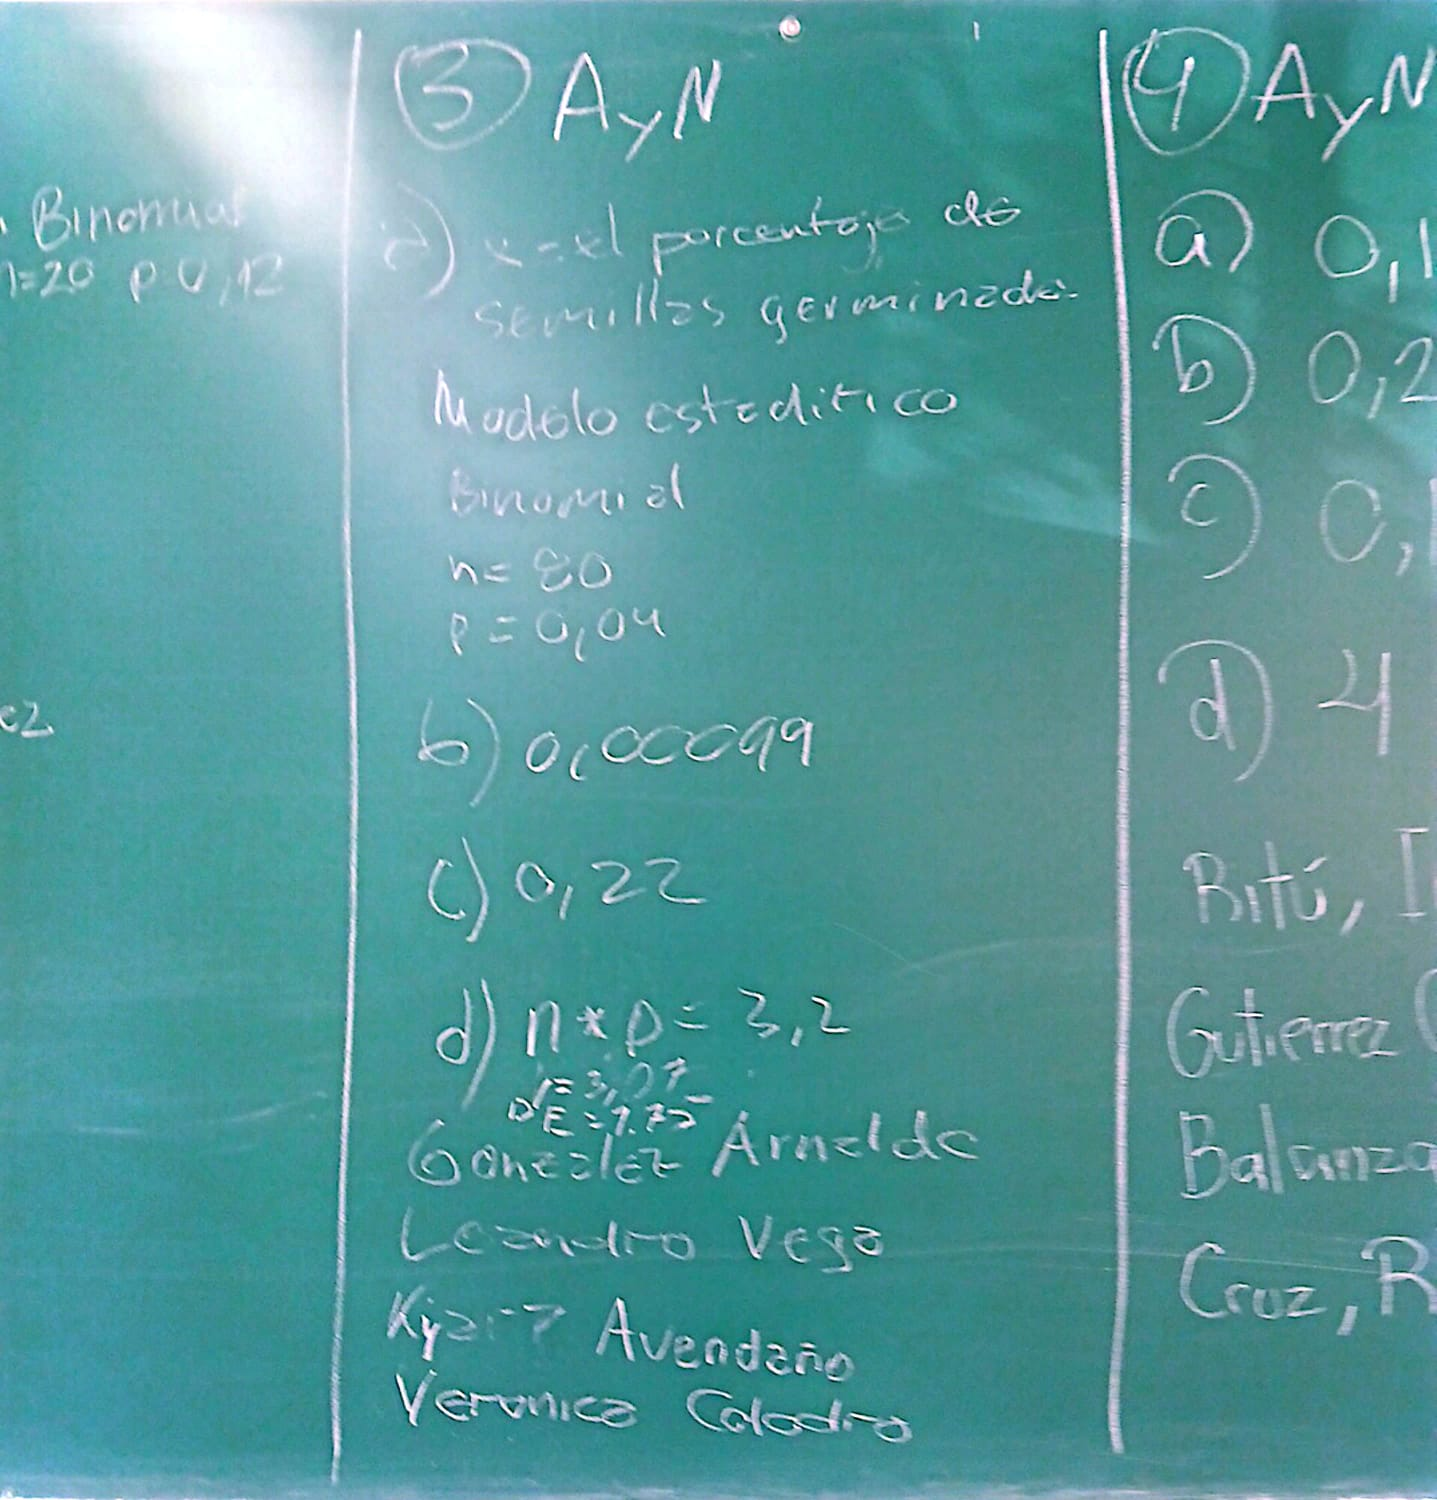
\includegraphics[width=0.4\linewidth,height=\textheight,keepaspectratio]{./IMAGENES/DISCRETAS/ej3-M.jpeg}

\begin{itemize}
\tightlist
\item
  \textbf{Candela Carrizo, Benjamín Gómez} (Ejercicio 1)

  \begin{itemize}
  \tightlist
  \item
    \begin{enumerate}
    \def\labelenumi{\alph{enumi})}
    \tightlist
    \item
      Modelo Binomial correcto: \texttt{n\ =\ 80}, \texttt{p\ =\ 0,04}.
      Variable aleatoria bien definida.
    \end{enumerate}
  \item
    \begin{enumerate}
    \def\labelenumi{\alph{enumi})}
    \setcounter{enumi}{1}
    \tightlist
    \item
      \texttt{P(X\ =\ 10)\ !=\ 0,99} (revisar decimales).
    \end{enumerate}
  \item
    \begin{enumerate}
    \def\labelenumi{\alph{enumi})}
    \setcounter{enumi}{2}
    \tightlist
    \item
      \texttt{P(X\ ≥\ 5)\ !=\ 0,94} (revisar los cálculos)
    \end{enumerate}
  \end{itemize}
\end{itemize}

\begin{Shaded}
\begin{Highlighting}[]
\NormalTok{n}\OtherTok{=}\DecValTok{80}\NormalTok{; p}\OtherTok{=}\FloatTok{0.04}
\DecValTok{1} \SpecialCharTok{{-}} \FunctionTok{pbinom}\NormalTok{(}\DecValTok{4}\NormalTok{, n, p) }\CommentTok{\# ¿por qué 4?}
\end{Highlighting}
\end{Shaded}

\begin{enumerate}
\def\labelenumi{\alph{enumi})}
\setcounter{enumi}{3}
\tightlist
\item
  No se pidió por falta de tiempo.
\end{enumerate}

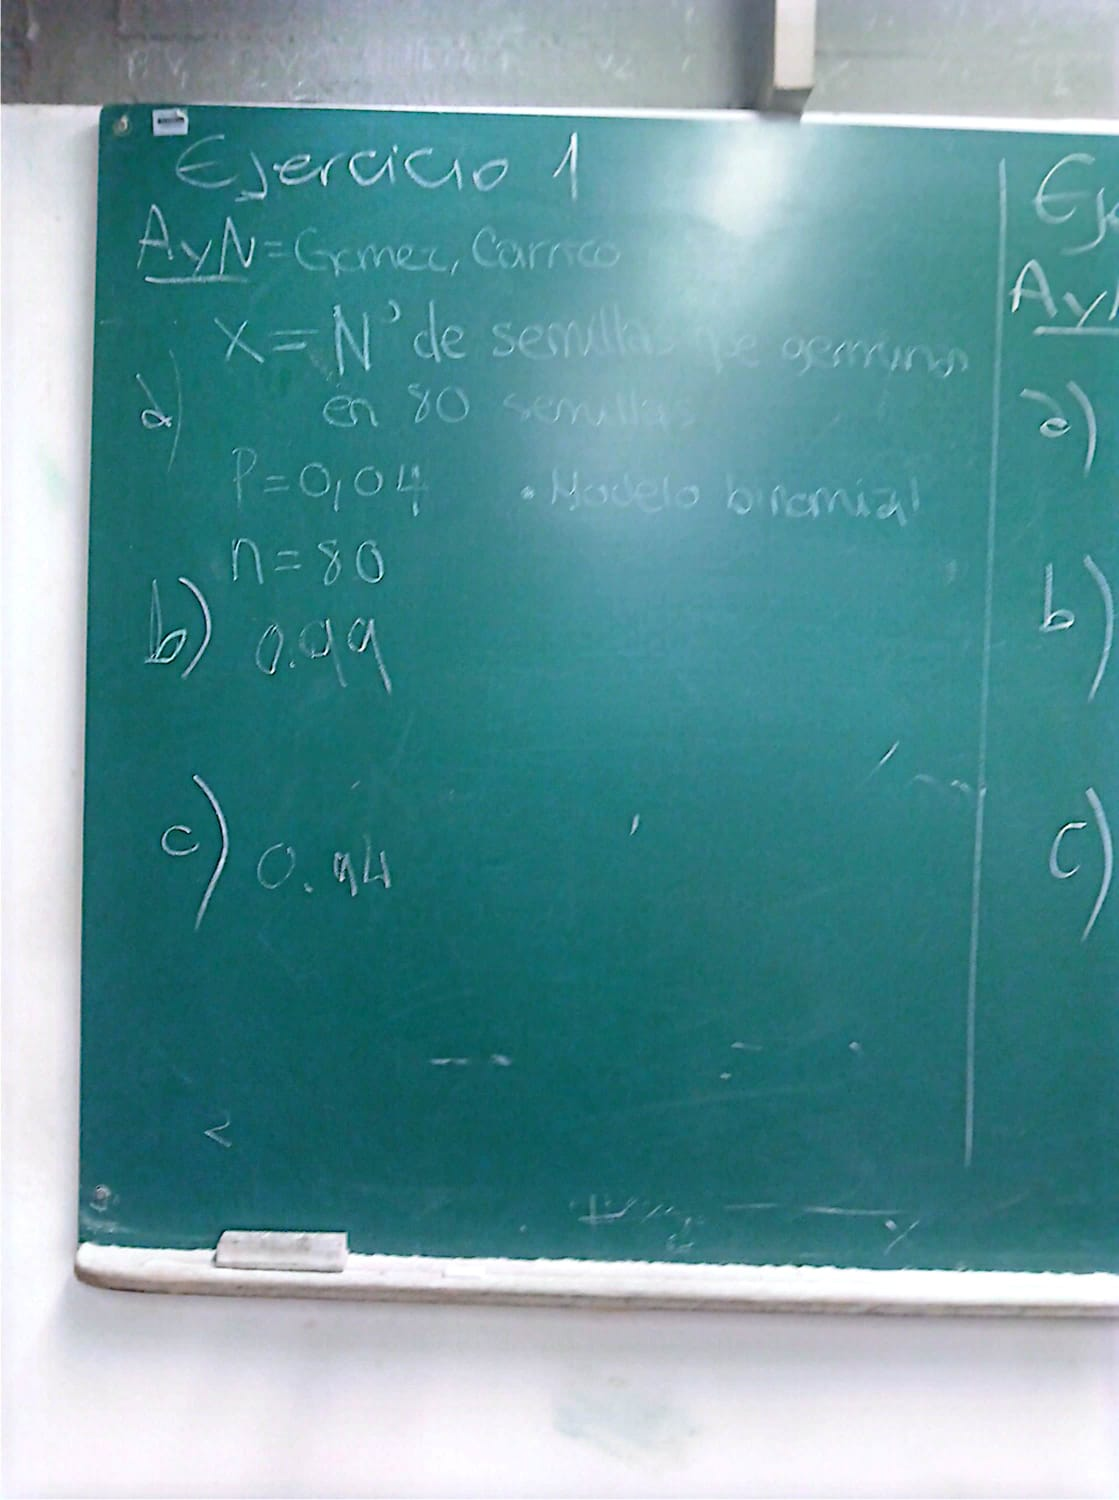
\includegraphics[width=0.4\linewidth,height=\textheight,keepaspectratio]{./IMAGENES/DISCRETAS/ej1-T.jpeg}

\begin{itemize}
\item
  \textbf{Julieta Martínez, Candela Díaz} (Ejercicio 2)

  \begin{itemize}
  \tightlist
  \item
    \begin{enumerate}
    \def\labelenumi{\alph{enumi})}
    \tightlist
    \item
      Modelo Binomial correcto: \texttt{n\ =\ 20}, \texttt{p\ =\ 0,12}.
    \end{enumerate}
  \item
    \begin{enumerate}
    \def\labelenumi{\alph{enumi})}
    \setcounter{enumi}{1}
    \tightlist
    \item
      \texttt{P(X\ =\ 0)\ =\ 0,0776} (correcto).
    \end{enumerate}
  \item
    \begin{enumerate}
    \def\labelenumi{\alph{enumi})}
    \setcounter{enumi}{2}
    \tightlist
    \item
      \texttt{0,6281} (correcto).
    \end{enumerate}
  \item
    \begin{enumerate}
    \def\labelenumi{\alph{enumi})}
    \setcounter{enumi}{3}
    \tightlist
    \item
      \texttt{0,0827} (correcto).
    \end{enumerate}
  \end{itemize}
\end{itemize}

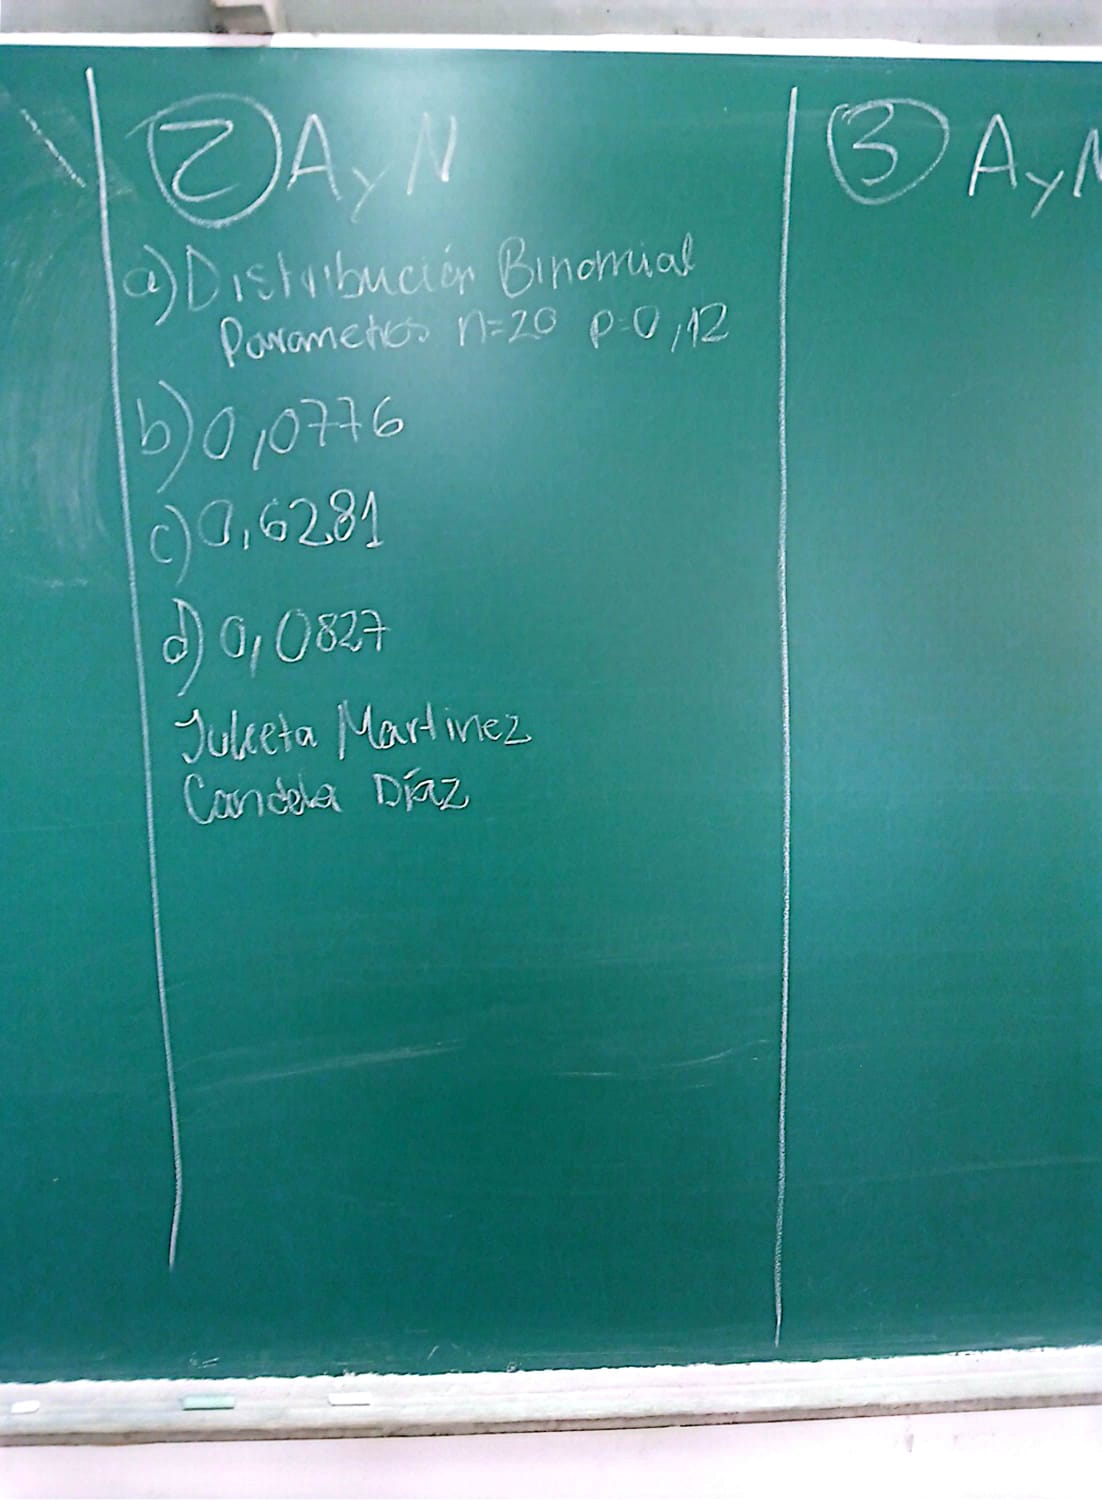
\includegraphics[width=0.4\linewidth,height=\textheight,keepaspectratio]{./IMAGENES/DISCRETAS/ej2-M.jpeg}

\begin{itemize}
\tightlist
\item
  \textbf{Marcelo, Gianella, Tania} (Ejercicio 2)

  \begin{itemize}
  \tightlist
  \item
    \begin{enumerate}
    \def\labelenumi{\alph{enumi})}
    \tightlist
    \item
      Modelo Binomial correcto: \texttt{n\ =\ 20}, \texttt{p\ =\ 0,12}.
    \end{enumerate}
  \item
    \begin{enumerate}
    \def\labelenumi{\alph{enumi})}
    \setcounter{enumi}{1}
    \tightlist
    \item
      \texttt{P(X\ =\ 0)\ =\ 0,0776} (faltó).
    \end{enumerate}
  \item
    \begin{enumerate}
    \def\labelenumi{\alph{enumi})}
    \setcounter{enumi}{2}
    \tightlist
    \item
      \texttt{2,0611e-09} (incorrecto: revisar el cálculo)
    \end{enumerate}
  \end{itemize}
\end{itemize}

\begin{Shaded}
\begin{Highlighting}[]
\NormalTok{n}\OtherTok{=}\DecValTok{20}\NormalTok{; p}\OtherTok{=}\FloatTok{0.12}
\FunctionTok{sum}\NormalTok{(}\FunctionTok{dbinom}\NormalTok{(}\DecValTok{2}\SpecialCharTok{:}\DecValTok{4}\NormalTok{,n,p))}
\CommentTok{\# o bien}
\FunctionTok{pbinom}\NormalTok{(}\DecValTok{4}\NormalTok{,n,p)}\SpecialCharTok{{-}}\FunctionTok{pbinom}\NormalTok{(}\DecValTok{1}\NormalTok{,n,p) }\CommentTok{\# ¿por qué 1?}
\end{Highlighting}
\end{Shaded}

\begin{itemize}
\tightlist
\item
  \begin{enumerate}
  \def\labelenumi{\alph{enumi})}
  \setcounter{enumi}{3}
  \tightlist
  \item
    \texttt{1,69e-05} (incorrecto). Revisar el cálculo:
    \texttt{1\ -\ pbinom(4,\ 20,\ 0.12)}.
  \end{enumerate}
\end{itemize}

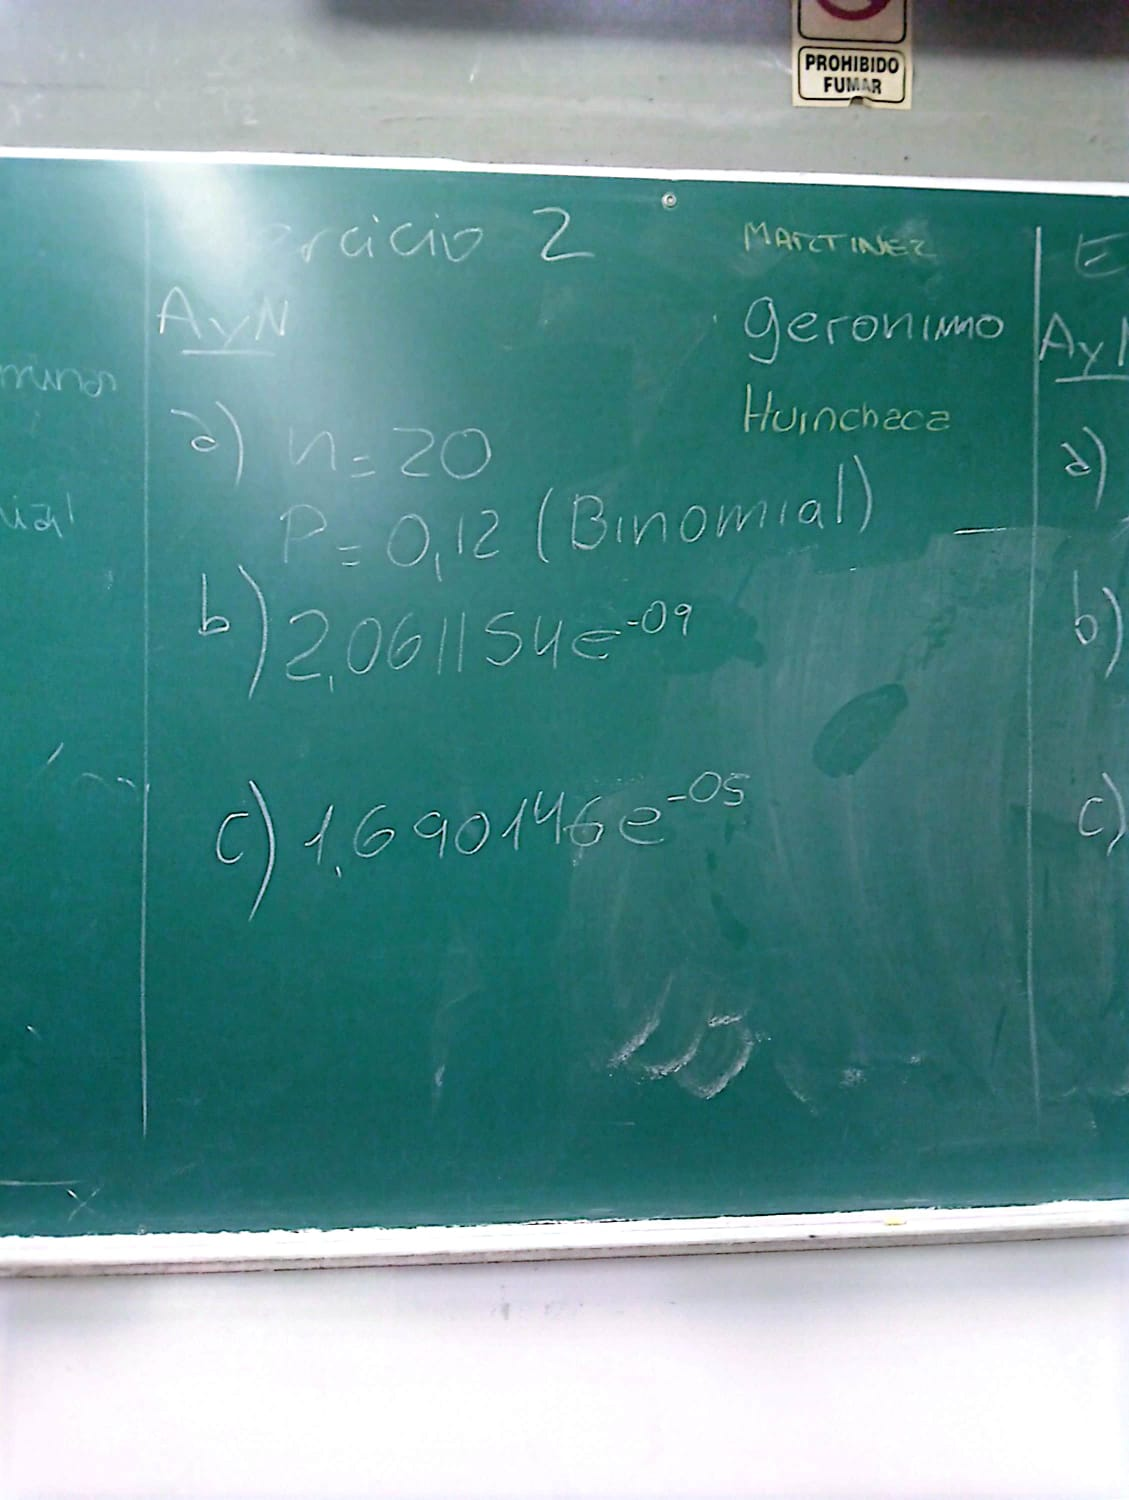
\includegraphics[width=0.4\linewidth,height=\textheight,keepaspectratio]{./IMAGENES/DISCRETAS/ej2-T.jpeg}

\begin{itemize}
\item
  \textbf{Mariela Lima, Jimena Garcia, Serena Chauque} (Ejercicio 3)

  \begin{itemize}
  \tightlist
  \item
    \begin{enumerate}
    \def\labelenumi{\alph{enumi})}
    \tightlist
    \item
      \texttt{P(Y\ =\ 4)\ =\ 0,189} (correcto; valor exacto 0,1898).
    \end{enumerate}
  \item
    \begin{enumerate}
    \def\labelenumi{\alph{enumi})}
    \setcounter{enumi}{1}
    \tightlist
    \item
      \texttt{P(Y\ ≤\ 2)\ =\ 0,17} (correcto; valor exacto 0,1736).
    \end{enumerate}
  \item
    \begin{enumerate}
    \def\labelenumi{\alph{enumi})}
    \setcounter{enumi}{2}
    \tightlist
    \item
      \texttt{P(Y\ \textgreater{}\ 6)\ =\ 0,16} (incorrecto, revisen los
      cálculos):
    \end{enumerate}
  \end{itemize}
\end{itemize}

\begin{Shaded}
\begin{Highlighting}[]
\NormalTok{lambda }\OtherTok{=} \FloatTok{4.5}
\DecValTok{1} \SpecialCharTok{{-}} \FunctionTok{ppois}\NormalTok{(}\DecValTok{5}\NormalTok{, lambda) }\CommentTok{\# ¿por qué 5?}
\end{Highlighting}
\end{Shaded}

\begin{enumerate}
\def\labelenumi{\alph{enumi})}
\setcounter{enumi}{3}
\tightlist
\item
  No se pidió por falta de tiempo.
\end{enumerate}

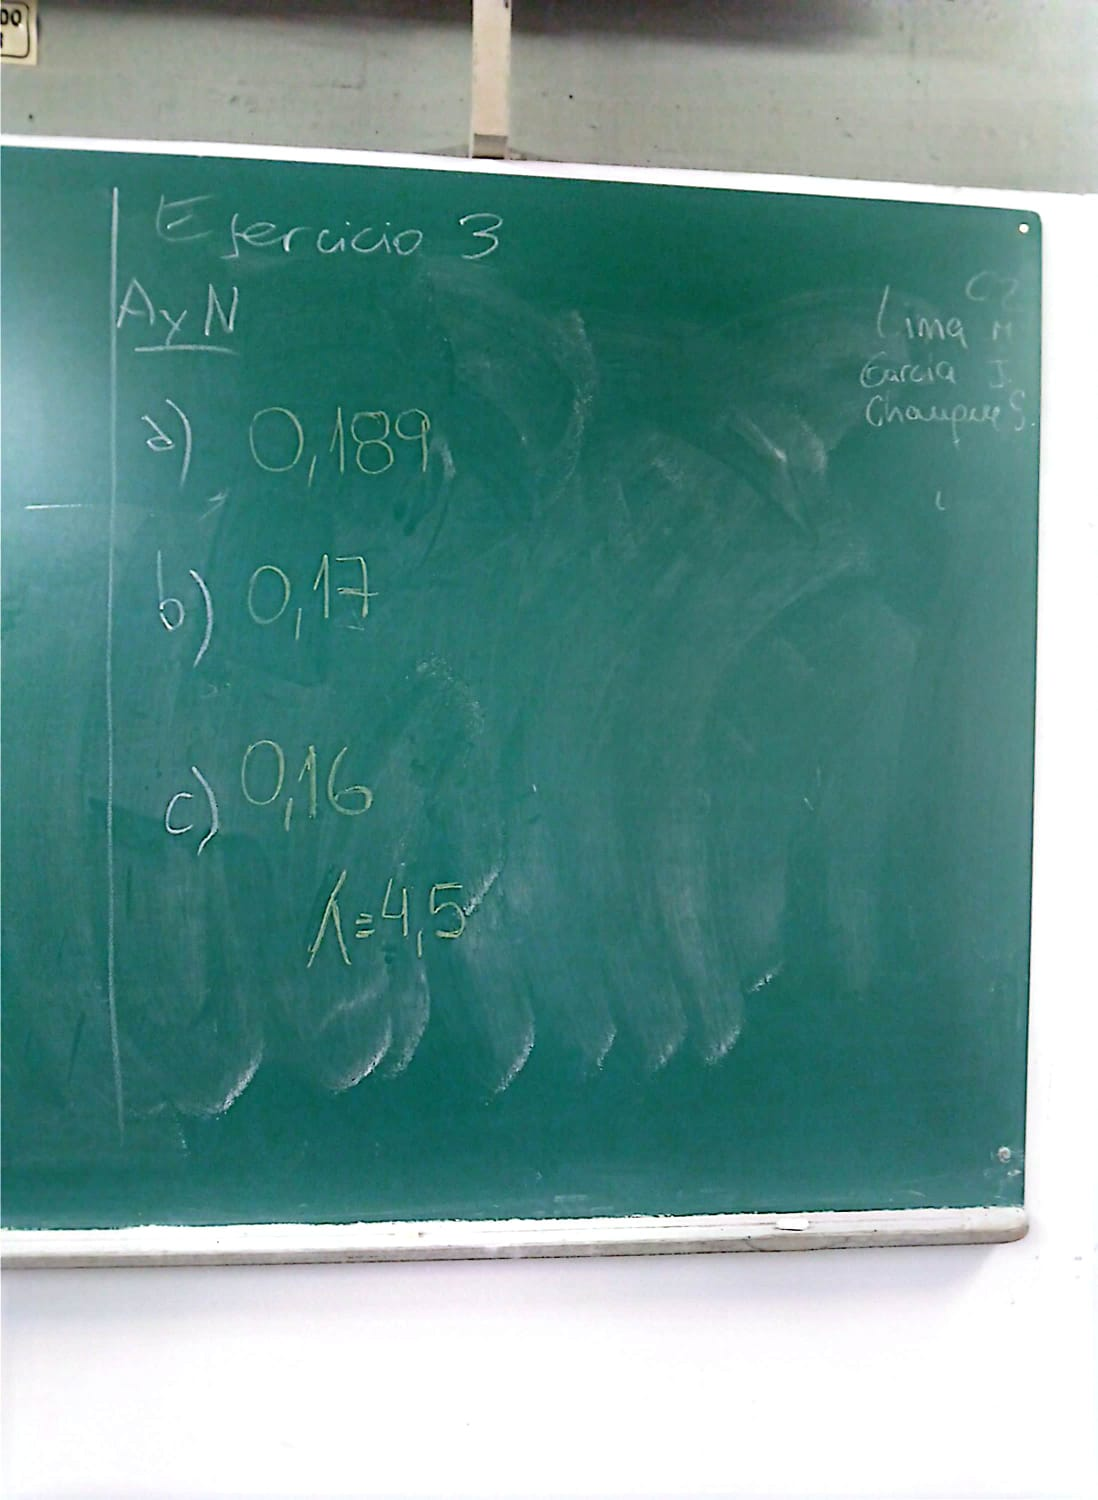
\includegraphics[width=0.4\linewidth,height=\textheight,keepaspectratio]{./IMAGENES/DISCRETAS/ej3-T.jpeg}

\begin{itemize}
\item
  \textbf{Irina Ritú, Cassandra Gutierrez Cortez, Iara Balanza, Rocío
  Cruz} (Ejercicio 4)

  \begin{itemize}
  \tightlist
  \item
    \begin{enumerate}
    \def\labelenumi{\alph{enumi})}
    \tightlist
    \item
      \texttt{P(Y\ =\ 0)\ =\ 0,16} (correcto, a 4 decimales es 0,1653,
      por lo tanto 0,17 a dos decimales).
    \end{enumerate}
  \item
    \begin{enumerate}
    \def\labelenumi{\alph{enumi})}
    \setcounter{enumi}{1}
    \tightlist
    \item
      \texttt{P(Y\ =\ 2)\ =\ 0,26} (correcto, pero el redondeo a dos
      decimales es 0,27, y a 4 decimales es 0,2678).
    \end{enumerate}
  \item
    \begin{enumerate}
    \def\labelenumi{\alph{enumi})}
    \setcounter{enumi}{2}
    \tightlist
    \item
      \texttt{P(Y\ \textgreater{}\ 3)\ =\ 0,10} (revisar los cálculos):
    \end{enumerate}
  \end{itemize}
\end{itemize}

\begin{Shaded}
\begin{Highlighting}[]
\NormalTok{lambda }\OtherTok{=} \FloatTok{1.8}
\DecValTok{1} \SpecialCharTok{{-}} \FunctionTok{ppois}\NormalTok{(}\DecValTok{2}\NormalTok{, lambda) }\CommentTok{\# ¿por qué 2 y no 3?}
\end{Highlighting}
\end{Shaded}

\begin{itemize}
\tightlist
\item
  \begin{enumerate}
  \def\labelenumi{\alph{enumi})}
  \setcounter{enumi}{3}
  \tightlist
  \item
    \texttt{4} (Correcto)
  \end{enumerate}
\end{itemize}

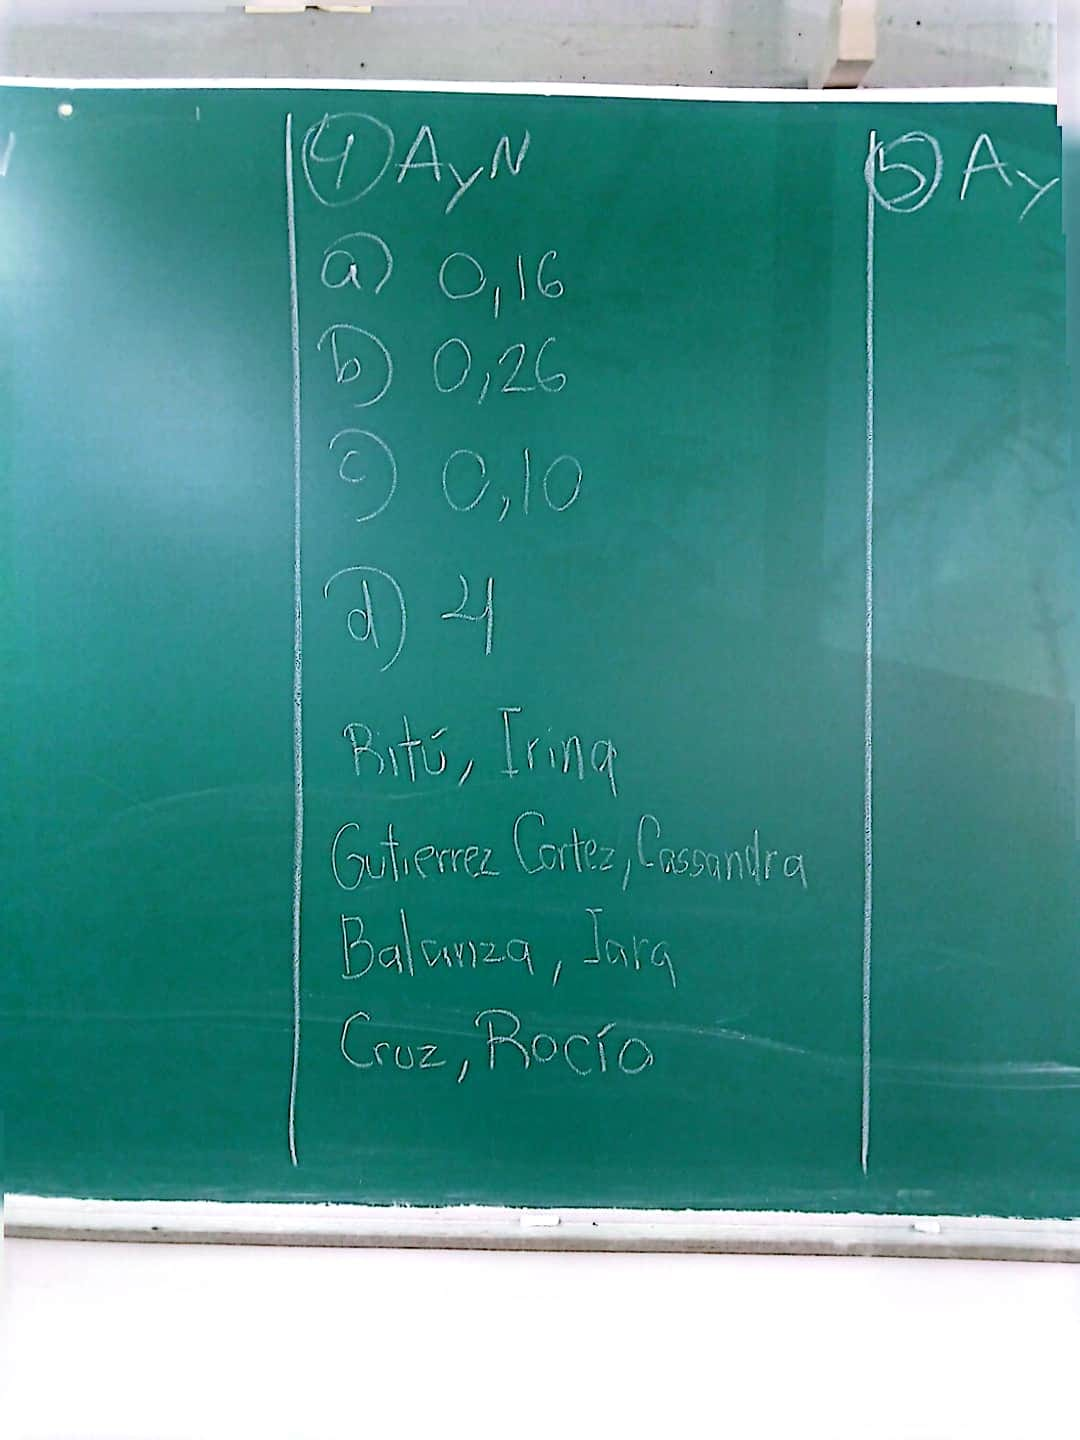
\includegraphics[width=0.4\linewidth,height=\textheight,keepaspectratio]{./IMAGENES/DISCRETAS/ej4-M.jpeg}

\section{Micro-ejercicios de aplicación
(optativos)}\label{micro-ejercicios-de-aplicaciuxf3n-optativos-3}

Los siguientes micro-ejercicios te permitirán practicar los conceptos
revisados en esta unidad. Puedes copiar y pegar las preguntas en un
script de R local, o bien utilizar \texttt{webR}, que es la versión
\emph{online} de R, disponible en esta guía.

\texttt{Nota}: los ejercicios están inspirados en trabajos científicos
publicados, pero contienen datos simulados. Por lo tanto, los resultados
obtenidos deben interpretarse únicamente con fines didácticos y no como
evidencia científica.

La finalidad es familiarizarse con el análisis estadístico y con el uso
de R a partir de situaciones similares a las que pueden encontrarse en
investigaciones reales.

\begin{Shaded}
\begin{Highlighting}[]

\CommentTok{\#  Instrucciones generales}
\CommentTok{\#  {-}{-}{-}{-}{-}{-}{-}{-}{-}{-}{-}{-}{-}{-}{-}{-}{-}{-}{-}{-}{-}{-}{-}}
\CommentTok{\#  En cada ejercicio:}
\CommentTok{\#    (a) identifique la variable aleatoria, el modelo probabilístico y sus parámetros}
\CommentTok{\#    (b) plantee la función de probabilidad y/o acumulada en notación estadística}
\CommentTok{\#    (c) seleccione e implemente la función de R correspondiente (dbinom, pbinom, qbinom, dpois, ppois, qpois)}
\CommentTok{\#    (d) interprete la probabilidad calculada, el cuantil o los parámetros en el contexto biológico}
\CommentTok{\#    (e) elabore una conclusión o síntesis en el contexto del problema ecológico / biológico}
\CommentTok{\#}
\CommentTok{\# =============================================================================}

\CommentTok{\#  Funciones disponibles (R base):}
\CommentTok{\#}
\CommentTok{\#    dbinom(x, size, prob)   \# Función de probabilidad de masa Binomial P(X = x)}
\CommentTok{\#    pbinom(q, size, prob)   \# Función de distribución acumulada Binomial P(X \textless{}= q)}
\CommentTok{\#    qbinom(p, size, prob)   \# Cuantil de la distribución Binomial}
\CommentTok{\#    rbinom(n, size, prob)   \# Generación de valores aleatorios Binomial}
\CommentTok{\#}
\CommentTok{\#    dpois(x, lambda)        \# Función de probabilidad de masa Poisson P(X = x)}
\CommentTok{\#    ppois(q, lambda)        \# Función de distribución acumulada Poisson P(X \textless{}= q)}
\CommentTok{\#    qpois(p, lambda)        \# Cuantil de la distribución Poisson}
\CommentTok{\#    rpois(n, lambda)        \# Generación de valores aleatorios Poisson}
\CommentTok{\#}
\CommentTok{\#    plot(x, y, ...)         \# Gráfico de puntos para distribuciones discretas}
\CommentTok{\#    barplot(height, ...)    \# Gráfico de barras para distribuciones discretas}
\CommentTok{\#    data.frame(...)         \# Tabla de datos para comparar modelos}
\CommentTok{\#}
\CommentTok{\#  Estadísticos "manuales" (esperanza y varianza):}
\CommentTok{\#    Esperanza Binomial:  E\_X = n * p}
\CommentTok{\#    Varianza Binomial:   Var\_X = n * p * (1 {-} p)}
\CommentTok{\#    Esperanza Poisson:   E\_X = lambda}
\CommentTok{\#    Varianza Poisson:    Var\_X = lambda}
\CommentTok{\#}
\CommentTok{\# =============================================================================}


\CommentTok{\# ─────────────────────────────────────────────────────────────────────────────}
\CommentTok{\#  SECCIÓN 1 — DISTRIBUCIÓN BINOMIAL}
\CommentTok{\# ─────────────────────────────────────────────────────────────────────────────}

\CommentTok{\# Ejercicio B1}
\CommentTok{\# {-}{-}{-}{-}{-}{-}{-}{-}{-}{-}{-}{-}}
\CommentTok{\# En un programa de conservación y restauración de bosques altoandinos en la}
\CommentTok{\# Puna jujeña (departamento Susques), se evalúa la capacidad germinativa}
\CommentTok{\# de semillas de Queñoa (Polylepis tomentella). En ensayos de laboratorio bajo}
\CommentTok{\# condiciones de temperatura y humedad reguladas, la probabilidad de que una}
\CommentTok{\# semilla viable germine con éxito a los 21 días es p = 0.25. Un biólogo coloca}
\CommentTok{\# n = 16 semillas en una bandeja experimental con sustrato estéril.}
\CommentTok{\#}
\CommentTok{\# a) ¿Cuál es la probabilidad de que germinen exactamente 4 semillas?}
\CommentTok{\# b) ¿Cuál es la probabilidad de que germinen a lo sumo 3 semillas?}
\CommentTok{\# c) ¿Cuál es la probabilidad de que germinen más de 6 semillas?}
\CommentTok{\# d) Calcule la esperanza matemática E(X), la varianza Var(X) y el desvío}
\CommentTok{\#    estándar σ(X) del número de semillas germinadas.}
\CommentTok{\# e) Mediante la función qbinom(), determine el número mínimo de semillas}
\CommentTok{\#    germinadas tal que la probabilidad acumulada sea de al menos 90\%.}

\CommentTok{\# Su código aquí:}


\CommentTok{\# Ejercicio B2}
\CommentTok{\# {-}{-}{-}{-}{-}{-}{-}{-}{-}{-}{-}{-}}
\CommentTok{\# En investigaciones de ecofisiología vegetal en la provincia fitogeográfica}
\CommentTok{\# del Monte en Mendoza, se analiza la tolerancia al estrés hídrico de plantines}
\CommentTok{\# de Jarilla (Larrea divaricata). Se sabe por antecedentes experimentales que}
\CommentTok{\# el 18\% (p = 0.18) de los plantines muestra síntomas de marchitamiento}
\CommentTok{\# permanente tras 20 días de privación severa de riego. Un equipo de campo}
\CommentTok{\# selecciona una muestra aleatoria independiente de n = 20 plantines.}
\CommentTok{\#}
\CommentTok{\# a) ¿Cuál es la probabilidad de que ningún plantín sufra marchitamiento?}
\CommentTok{\# b) ¿Cuál es la probabilidad de que entre 2 y 5 plantines (inclusive)}
\CommentTok{\#    manifiesten marchitamiento permanente?}
\CommentTok{\# c) ¿Cuál es la probabilidad de que al menos 4 plantines se marchiten?}
\CommentTok{\# d) Grafique la función de probabilidad de masa completa P(X = x) para}
\CommentTok{\#    x = 0, 1, ..., 20 utilizando la función barplot() o plot(), agregando}
\CommentTok{\#    títulos y etiquetas claras en los ejes.}

\CommentTok{\# Su código aquí:}


\CommentTok{\# Ejercicio B3}
\CommentTok{\# {-}{-}{-}{-}{-}{-}{-}{-}{-}{-}{-}{-}}
\CommentTok{\# Durante campañas de monitoreo parasitológico e higiene biológica en la}
\CommentTok{\# Reserva de Biósfera Laguna de los Pozuelos, investigadores de la UNJu}
\CommentTok{\# evalúan la presencia de hemoparásitos en vicuñas (Vicugna vicugna) capturadas}
\CommentTok{\# temporalmente para esquila ecosustentable. Históricamente, el 12\% de los}
\CommentTok{\# individuos adultos presenta infección por protozoos sanguíneos. En una}
\CommentTok{\# jornada de muestreo se analiza la sangre de n = 15 vicuñas.}
\CommentTok{\#}
\CommentTok{\# a) ¿Cuál es la probabilidad de que exactamente 2 vicuñas presenten}
\CommentTok{\#    hemoparásitos?}
\CommentTok{\# b) ¿Cuál es la probabilidad de que a lo sumo 1 vicuña esté infectada?}
\CommentTok{\# c) ¿Cuál es la probabilidad de encontrar 3 o más vicuñas infectadas en}
\CommentTok{\#    el grupo?}
\CommentTok{\# d) Si el protocolo sanitario establece alerta epidemiológica cuando más de}
\CommentTok{\#    4 individuos resultan positivos, ¿cuál es la probabilidad de activar dicha}
\CommentTok{\#    alerta en esta muestra?}
\CommentTok{\# e) Calcule E(X) y σ(X) e interprete biológicamente el resultado.}

\CommentTok{\# Su código aquí:}


\CommentTok{\# Ejercicio B4}
\CommentTok{\# {-}{-}{-}{-}{-}{-}{-}{-}{-}{-}{-}{-}}
\CommentTok{\# Un estudio entomológico en la Quebrada de Humahuaca examina el grado de}
\CommentTok{\# agallamiento foliar causado por dípteros cecidógenos en Aguaribay (Schinus}
\CommentTok{\# molle). La probabilidad de que un folíolo tomado al azar presente al menos una}
\CommentTok{\# agalla bien desarrollada es p = 0.30. Un investigador examina n = 12}
\CommentTok{\# folíolos de un fuste principal.}
\CommentTok{\#}
\CommentTok{\# a) ¿Cuál es la probabilidad de encontrar exactamente 3 folíolos agallados?}
\CommentTok{\# b) ¿Cuál es la probabilidad de que menos de 3 folíolos presenten agallas?}
\CommentTok{\# c) ¿Cuál es la probabilidad de que al menos la mitad de los folíolos}
\CommentTok{\#    (6 o más) estén afectados?}
\CommentTok{\# d) Obtenga el cuantil del 95\% de la distribución con qbinom() e interprete}
\CommentTok{\#    qué representa este valor en el contexto del daño foliar.}

\CommentTok{\# Su código aquí:}


\CommentTok{\# Ejercicio B5}
\CommentTok{\# {-}{-}{-}{-}{-}{-}{-}{-}{-}{-}{-}{-}}
\CommentTok{\# En estudios demográficos de aves rapaces neotropicales, se realiza el sexado molecular de}
\CommentTok{\# pichones de Cóndor Andino (Vultur gryphus). Suponiendo una proporción de}
\CommentTok{\# sexos 1:1 en el momento de la eclosión (p = 0.50 para hembras), se analizan}
\CommentTok{\# n = 10 pichones nacidos en la presente temporada reproductiva.}
\CommentTok{\#}
\CommentTok{\# a) ¿Cuál es la probabilidad de que exactamente 5 pichones sean hembras?}
\CommentTok{\# b) ¿Cuál es la probabilidad de que el número de hembras se encuentre entre}
\CommentTok{\#    4 y 6 (inclusive)?}
\CommentTok{\# c) ¿Cuál es la probabilidad de observar un sesgo severo con más de 7 hembras?}
\CommentTok{\# d) Calcule la esperanza matemática y la varianza de la variable aleatoria X}
\CommentTok{\#    (número de pichones hembra en la nidada).}

\CommentTok{\# Su código aquí:}


\CommentTok{\# Ejercicio B6}
\CommentTok{\# {-}{-}{-}{-}{-}{-}{-}{-}{-}{-}{-}{-}}
\CommentTok{\# En poblaciones naturales de anfibios de las Yungas jujeñas, la frecuencia}
\CommentTok{\# de un alelo recesivo que produce una coloración melánica atípica en el Sapo}
\CommentTok{\# de Yunga (Rhinella rumbolli) genera una prevalencia del fenotipo del 8\%}
\CommentTok{\# (p = 0.08) en estados larvarios. Se recolecta una muestra al azar de}
\CommentTok{\# n = 25 renacuajos en un cuerpo de agua semipermanente.}
\CommentTok{\#}
\CommentTok{\# a) ¿Cuál es la probabilidad de que ninguno de los renacuajos muestre el}
\CommentTok{\#    fenotipo melánico?}
\CommentTok{\# b) ¿Cuál es la probabilidad de que exactamente 2 renacuajos sean melánicos?}
\CommentTok{\# c) ¿Cuál es la probabilidad de hallar al menos 3 renacuajos melánicos?}
\CommentTok{\# d) Determine la mediana de la distribución utilizando qbinom(0.5, ...).}
\CommentTok{\# e) Calcule el valor esperado E(X) y el desvío estándar σ(X) de renacuajos}
\CommentTok{\#    melánicos en muestras de este tamaño.}

\CommentTok{\# Su código aquí:}


\CommentTok{\# ─────────────────────────────────────────────────────────────────────────────}
\CommentTok{\#  SECCIÓN 2 — DISTRIBUCIÓN DE POISSON}
\CommentTok{\# ─────────────────────────────────────────────────────────────────────────────}

\CommentTok{\# Ejercicio P1}
\CommentTok{\# {-}{-}{-}{-}{-}{-}{-}{-}{-}{-}{-}{-}}
\CommentTok{\# En evaluaciones de la calidad ecológica de cursos de agua de montaña en el}
\CommentTok{\# Río Grande (sector Tilcara), se utiliza el recuento de ninfas de insectos}
\CommentTok{\# acuáticos del orden Ephemeroptera como bioindicador de aguas oligotróficas.}
\CommentTok{\# Los muestreos históricos con red de Surber (superficie estándar de 0.1 m²)}
\CommentTok{\# indican un promedio de λ = 4.2 ninfas por unidad de muestra.}
\CommentTok{\#}
\CommentTok{\# a) ¿Cuál es la probabilidad de que en una muestra de 0.1 m² no se registre}
\CommentTok{\#    ninguna ninfa de Ephemeroptera?}
\CommentTok{\# b) ¿Cuál es la probabilidad de encontrar exactamente 4 ninfas en la muestra?}
\CommentTok{\# c) ¿Cuál es la probabilidad de encontrar más de 6 ninfas en esa misma área?}
\CommentTok{\# d) Si el área de muestreo se duplica a 0.2 m² (parámetro λ\_nuevo = 8.4),}
\CommentTok{\#    ¿cuál es la probabilidad de encontrar al menos 5 ninfas de Ephemeroptera?}

\CommentTok{\# Su código aquí:}


\CommentTok{\# Ejercicio P2}
\CommentTok{\# {-}{-}{-}{-}{-}{-}{-}{-}{-}{-}{-}{-}}
\CommentTok{\# Durante monitoreos de biodiversidad nocturna de mamíferos voladores en la}
\CommentTok{\# selva pedemontana del Parque Nacional Calilegua, se utilizan redes de niebla}
\CommentTok{\# para capturar murciélagos frugívoros (Sturnira lilium). En un intervalo de}
\CommentTok{\# muestreo estándar de 4 horas, se registra un promedio de λ = 2.5 capturas por}
\CommentTok{\# red desplegada.}
\CommentTok{\#}
\CommentTok{\# a) ¿Cuál es la probabilidad de que en una red no se capture ningún individuo}
\CommentTok{\#    durante el período de muestreo?}
\CommentTok{\# b) ¿Cuál es la probabilidad de capturar entre 2 y 4 murciélagos (inclusive)?}
\CommentTok{\# c) ¿Cuál es la probabilidad de que se capturen más de 5 individuos en una red?}
\CommentTok{\# d) Utilizando la función qpois(), determine el número de capturas X a partir}
\CommentTok{\#    del cual se acumula al menos el 90\% de probabilidad.}

\CommentTok{\# Su código aquí:}


\CommentTok{\# Ejercicio P3}
\CommentTok{\# {-}{-}{-}{-}{-}{-}{-}{-}{-}{-}{-}{-}}
\CommentTok{\# En investigaciones liquenológicas sobre fustes de Aliso del Cerro (Alnus}
\CommentTok{\# acuminata) en los bosques montanos de Yala, se cuenta la densidad de talos}
\CommentTok{\# de líquenes crustosos por cuadrícula de madera de 10 cm x 10 cm. El promedio}
\CommentTok{\# observado es de λ = 3.6 talos por cuadrícula.}
\CommentTok{\#}
\CommentTok{\# a) ¿Cuál es la probabilidad de observar una cuadrícula completamente limpia}
\CommentTok{\#    sin ningún talo (X = 0)?}
\CommentTok{\# b) ¿Cuál es la probabilidad de hallar exactamente 3 talos de liquen?}
\CommentTok{\# c) ¿Cuál es la probabilidad de hallar 6 o más talos en una cuadrícula?}
\CommentTok{\# d) Grafique la función de probabilidad de Poisson para λ = 3.6 en el rango}
\CommentTok{\#    x = 0, 1, ..., 12 mediante barplot() o plot(), identificando la moda.}

\CommentTok{\# Su código aquí:}


\CommentTok{\# Ejercicio P4}
\CommentTok{\# {-}{-}{-}{-}{-}{-}{-}{-}{-}{-}{-}{-}}
\CommentTok{\# En el laboratorio de microbiología ambiental de la FCA{-}UNJu, se efectúa el}
\CommentTok{\# recuento de bacterias solubilizadoras de fósforo (Pseudomonas fluorescens) en}
\CommentTok{\# placas Petri con agar selectivo, a partir de diluciones de suelo forestal de}
\CommentTok{\# Yungas. El recuento promedio por campo microscópico es de λ = 5.0 colonias.}
\CommentTok{\#}
\CommentTok{\# a) ¿Cuál es la probabilidad de observar exactamente 5 colonias en un campo?}
\CommentTok{\# b) ¿Cuál es la probabilidad de observar menos de 3 colonias (X \textless{}= 2)?}
\CommentTok{\# c) ¿Cuál es la probabilidad de observar más de 8 colonias en un campo?}
\CommentTok{\# d) ¿Cuál es el valor más probable (moda) de la distribución? Verifique su}
\CommentTok{\#    respuesta calculando dpois(4:6, lambda = 5.0).}

\CommentTok{\# Su código aquí:}


\CommentTok{\# Ejercicio P5}
\CommentTok{\# {-}{-}{-}{-}{-}{-}{-}{-}{-}{-}{-}{-}}
\CommentTok{\# En estudios de conservación de ungulados autóctonos amenazados en los}
\CommentTok{\# pastizales de neblina de las Serranías de Zapla, se realiza el registro de}
\CommentTok{\# huellas de Taruca (Hippocamelus antisensis) sobre transectas de 500 metros.}
\CommentTok{\# La tasa promedio de avistamiento de pisadas frescas es de λ = 1.8 pisadas por}
\CommentTok{\# transecta.}
\CommentTok{\#}
\CommentTok{\# a) ¿Cuál es la probabilidad de recorre una transecta de 500 m y no hallar}
\CommentTok{\#    ninguna pisada de Taruca?}
\CommentTok{\# b) ¿Cuál es la probabilidad de registrar exactamente 2 pisadas?}
\CommentTok{\# c) Si la transecta se extiende a 1000 metros (distancia doble, λ = 3.6),}
\CommentTok{\#    ¿cuál es la probabilidad de registrar más de 4 pisadas?}
\CommentTok{\# d) Verifique cuantitativamente que para la distribución de Poisson la}
\CommentTok{\#    esperanza matemática E(X) es igual a la varianza Var(X).}

\CommentTok{\# Su código aquí:}


\CommentTok{\# Ejercicio P6}
\CommentTok{\# {-}{-}{-}{-}{-}{-}{-}{-}{-}{-}{-}{-}}
\CommentTok{\# En renovales de Cedro Coya (Cedrela lilloi) bajo dosel forestal en las}
\CommentTok{\# Yungas de Jujuy, la ocurrencia de perforaciones foliares producidas por}
\CommentTok{\# coleópteros defoliadores sigue un proceso de Poisson con una media de}
\CommentTok{\# λ = 2.2 perforaciones por hoja compuesta.}
\CommentTok{\#}
\CommentTok{\# a) ¿Cuál es la probabilidad de que una hoja no presente ninguna perforación?}
\CommentTok{\# b) ¿Cuál es la probabilidad de que una hoja compuesta tenga entre 1 y 3}
\CommentTok{\#    perforaciones (inclusive)?}
\CommentTok{\# c) ¿Cuál es la probabilidad de encontrar más de 5 perforaciones en una hoja?}
\CommentTok{\# d) En una rama que contiene 5 hojas compuestas (intervalo acumulado de}
\CommentTok{\#    λ\_total = 11.0), ¿cuál es la probabilidad de contar a lo sumo 8}
\CommentTok{\#    perforaciones en total?}

\CommentTok{\# Su código aquí:}


\CommentTok{\# ─────────────────────────────────────────────────────────────────────────────}
\CommentTok{\#  SECCIÓN 3 — APROXIMACIÓN BINOMIAL–POISSON}
\CommentTok{\# ─────────────────────────────────────────────────────────────────────────────}
\CommentTok{\#}
\CommentTok{\#  Condiciones de aplicabilidad:}
\CommentTok{\#    · Tamaño muestral grande (n \textgreater{}= 100, o n \textgreater{}= 50 si p es muy pequeño)}
\CommentTok{\#    · Probabilidad de éxito muy pequeña (p \textless{}= 0.05, "eventos raros")}
\CommentTok{\#    · Parámetro de tasa moderado (λ = n * p \textless{} 10)}
\CommentTok{\#}
\CommentTok{\#  En cada ejercicio:}
\CommentTok{\#    (i)   verifique el cumplimiento de los supuestos para la aproximación}
\CommentTok{\#    (ii)  calcule la probabilidad mediante la aproximación de Poisson P(λ)}
\CommentTok{\#    (iii) calcule la probabilidad exacta mediante la Binomial Bi(n, p)}
\CommentTok{\#    (iv)  compare ambos resultados y evalúe la calidad de la aproximación}


\CommentTok{\# Ejercicio A1}
\CommentTok{\# {-}{-}{-}{-}{-}{-}{-}{-}{-}{-}{-}{-}}
\CommentTok{\# En investigaciones de genética forestal sobre especies autóctonas del NOA,}
\CommentTok{\# la frecuencia de mutaciones clorofílicas espontáneas (albinismo parcial) en}
\CommentTok{\# la germinación de Lapacho Amarillo (Tabebuia serratifolia) es de p = 0.015.}
\CommentTok{\# Un biólogo examina un lote de n = 200 plántulas recién germinadas.}
\CommentTok{\#}
\CommentTok{\# a) Verifique las condiciones de aplicabilidad de la aproximación de Poisson}
\CommentTok{\#    e indique el parámetro λ = n * p.}
\CommentTok{\# b) Utilizando la aproximación de Poisson P(λ), calcule P(X = 0), P(X \textless{}= 2)}
\CommentTok{\#    y P(X \textgreater{}= 4).}
\CommentTok{\# c) Utilizando la distribución Binomial exacta Bi(200, 0.015), calcule los}
\CommentTok{\#    mismos valores de probabilidad.}
\CommentTok{\# d) Compare numéricamente ambos métodos e interprete la exactitud de la}
\CommentTok{\#    aproximación para la toma de decisiones ecológicas.}

\CommentTok{\# Su código aquí:}


\CommentTok{\# Ejercicio A2}
\CommentTok{\# {-}{-}{-}{-}{-}{-}{-}{-}{-}{-}{-}{-}}
\CommentTok{\# En el vivero de la FCA{-}UNJu, se evalúa la susceptibilidad de alvéolos de}
\CommentTok{\# inoculación de Aliso del Cerro (Alnus acuminata) al ataque de oomicetes}
\CommentTok{\# patógenos del género Phytophthora. La probabilidad de infección individual en}
\CommentTok{\# alvéolos bajo condiciones controladas es de p = 0.02. Se inspecciona una}
\CommentTok{\# bandeja forestal con n = 150 alvéolos.}
\CommentTok{\#}
\CommentTok{\# a) Verifique los requisitos para aproximar por Poisson y calcule λ.}
\CommentTok{\# b) Mediante la aproximación de Poisson, calcule P(X = 0), P(X = 1) y}
\CommentTok{\#    P(X \textgreater{}= 3).}
\CommentTok{\# c) Mediante la distribución Binomial exacta, calcule las mismas}
\CommentTok{\#    probabilidades.}
\CommentTok{\# d) Construya una tabla comparativa en R utilizando la función data.frame()}
\CommentTok{\#    con las columnas: x, Binomial\_Exacta, Poisson\_Aproximada y Diferencia.}

\CommentTok{\# Su código aquí:}


\CommentTok{\# Ejercicio A3}
\CommentTok{\# {-}{-}{-}{-}{-}{-}{-}{-}{-}{-}{-}{-}}
\CommentTok{\# En estudios de contaminación por microplásticos en la cuenca del Río San}
\CommentTok{\# Francisco (Jujuy), la probabilidad de que una mojarra (Sproattus spp.)}
\CommentTok{\# contenga fibras de microplástico en su estómago en tramos de cabecera es de}
\CommentTok{\# p = 0.025. Se disecan n = 120 ejemplares capturados durante una campaña.}
\CommentTok{\#}
\CommentTok{\# a) Verifique las condiciones de la aproximación e indique λ = n * p.}
\CommentTok{\# b) Con la aproximación de Poisson, calcule P(X \textless{}= 2) y P(X \textgreater{}= 5).}
\CommentTok{\# c) Con la distribución Binomial exacta, calcule los mismos valores.}
\CommentTok{\# d) Calcule el error relativo porcentual en la estimación de P(X \textless{}= 2)}
\CommentTok{\#    definido como |P\_pois {-} P\_binom| / P\_binom * 100.}

\CommentTok{\# Su código aquí:}


\CommentTok{\# Ejercicio A4}
\CommentTok{\# {-}{-}{-}{-}{-}{-}{-}{-}{-}{-}{-}{-}}
\CommentTok{\# En controles de calidad de formulaciones bioplaguicidas a base de Bacillus}
\CommentTok{\# thuringiensis para el control de larvas de insectos en cultivos de la}
\CommentTok{\# Quebrada de Humahuaca, la probabilidad de encontrar una espora atípica no}
\CommentTok{\# viable en alícuotas microscópicas es de p = 0.01. Se analizan n = 250}
\CommentTok{\# alícuotas independientes.}
\CommentTok{\#}
\CommentTok{\# a) Indique los parámetros n y p de la Binomial y determine el valor de λ}
\CommentTok{\#    para la aproximación de Poisson.}
\CommentTok{\# b) Usando la Poisson aproximada, calcule la probabilidad de observar}
\CommentTok{\#    exactamente 0, 1, 2 y 3 esporas atípicas.}
\CommentTok{\# c) Usando la Binomial exacta, calcule las mismas probabilidades.}
\CommentTok{\# d) Si el criterio de rechazo del lote biológico requiere encontrar 5 o más}
\CommentTok{\#    esporas atípicas (X \textgreater{}= 5), calcule la probabilidad de rechazo con ambos}
\CommentTok{\#    modelos y determine si la decisión técnica se altera.}

\CommentTok{\# Su código aquí:}


\CommentTok{\# Ejercicio A5}
\CommentTok{\# {-}{-}{-}{-}{-}{-}{-}{-}{-}{-}{-}{-}}
\CommentTok{\# En relictos de bosques de Polylepis pepei en ambientes de alta montaña en la}
\CommentTok{\# Puna de Jujuy, la aparición de malformaciones foliares teratológicas debidas}
\CommentTok{\# a daño por congelamiento extremo tiene una probabilidad de p = 0.03. Se}
\CommentTok{\# inspecciona una muestra de n = 100 plántulas en una ladera expuesta.}
\CommentTok{\#}
\CommentTok{\# a) Verifique si se cumplen los supuestos para la aproximación de Poisson e}
\CommentTok{\#    indique el parámetro λ.}
\CommentTok{\# b) Mediante la distribución de Poisson, calcule P(X \textless{}= 1), P(X = 3) y}
\CommentTok{\#    P(X \textgreater{}= 4).}
\CommentTok{\# c) Mediante la distribución Binomial exacta, calcule las mismas}
\CommentTok{\#    probabilidades.}
\CommentTok{\# d) Elabore un gráfico comparativo de barras utilizando barplot() para}
\CommentTok{\#    x = 0, 1, ..., 8 contrastando dpois(0:8, lambda) y dbinom(0:8, 100, 0.03).}

\CommentTok{\# Su código aquí:}


\CommentTok{\# Ejercicio A6}
\CommentTok{\# {-}{-}{-}{-}{-}{-}{-}{-}{-}{-}{-}{-}}
\CommentTok{\# En monitoreos parasitológicos e histopatológicos de la Trucha Marrón (Salmo}
\CommentTok{\# trutta) introducida en arroyos de la cuenca de Yala, la presencia de cuerpos}
\CommentTok{\# de inclusión virales en cortes histológicos de tejido hepático ocurre con}
\CommentTok{\# una probabilidad de p = 0.008. Un equipo examina n = 300 cortes.}
\CommentTok{\#}
\CommentTok{\# a) Verifique los requisitos para aproximar por Poisson y determine λ.}
\CommentTok{\# b) Utilizando la aproximación de Poisson, calcule P(X = 0), P(X = 2) y}
\CommentTok{\#    P(X \textgreater{}= 3).}
\CommentTok{\# c) Utilizando la distribución Binomial exacta, calcule los mismos valores.}
\CommentTok{\# d) Calcule la probabilidad de encontrar entre 1 y 4 cortes afectados}
\CommentTok{\#    (inclusive) según ambos modelos y comente el grado de concordancia.}

\CommentTok{\# Su código aquí:}


\CommentTok{\# =============================================================================}
\end{Highlighting}
\end{Shaded}

\bookmarksetup{startatroot}

\chapter{Trabajo Práctico 4: Distribución
Normal}\label{trabajo-pruxe1ctico-4-distribuciuxf3n-normal}

Objetivos del Trabajo Práctico El trabajo práctico tiene como objetivos:
(1) Reconocer situaciones en las que una variable biológica o ambiental
continua puede modelarse adecuadamente mediante una distribución Normal,
identificando sus parámetros (μ y σ); (2) Interpretar los parámetros de
la distribución Normal en términos de la ubicación (media) y la
dispersión (desvío estándar) del fenómeno bajo estudio; (3) Calcular e
interpretar probabilidades acumuladas, de intervalo y cuantiles a partir
de la función de distribución Normal, utilizando las funciones pnorm() y
qnorm() de R; (4) Aplicar la estandarización (transformación Z) de forma
manual y contrastarla con el cálculo directo en la escala original
mediante R; (5) Simular observaciones de una variable Normal con rnorm()
y contrastar las propiedades empíricas de la distribución (regla
empírica 68-95-99,7\%) con los resultados teóricos; y (6) Interpretar
los resultados probabilísticos obtenidos en el marco de la práctica
profesional en Ciencias Biológicas.

\begin{tcolorbox}[enhanced jigsaw, arc=.35mm, bottomrule=.15mm, bottomtitle=1mm, breakable, colback=white, colbacktitle=quarto-callout-important-color!10!white, colframe=quarto-callout-important-color-frame, coltitle=black, left=2mm, leftrule=.75mm, opacityback=0, opacitybacktitle=0.6, rightrule=.15mm, title=\textcolor{quarto-callout-important-color}{\faExclamation}\hspace{0.5em}{Lectura Sugerida para el Trabajo Práctico}, titlerule=0mm, toprule=.15mm, toptitle=1mm]

Se recomienda a los estudiantes consultar el libro \textbf{«Apuntes de
Bioestadística. Con ejercicios resueltos»} para profundizar los
conceptos teóricos y metodológicos desarrollados en este marco:

\begin{itemize}
\tightlist
\item
  \textbf{Unidad 6: Distribución Normal}: Consultar la definición formal
  de la distribución, sus parámetros (μ, σ) y sus propiedades
  características (simetría, campo de definición, curtosis constante),
  así como la transformación de estandarización o tipificación (Z).
\item
  \textbf{Unidad 6: Cálculo de Probabilidades y Cuantiles}: Revisar el
  uso de la función de distribución acumulada para el cálculo de
  probabilidades de cola e intervalo, la obtención de cuantiles, y las
  propiedades empíricas de la distribución Normal (68-95-99,7\%).
\end{itemize}

Como lecturas complementarias, se sugiere también revisar la unidad
\emph{«Modelos probabilísticos»} del libro \textbf{«Estadística y
Biometría»} de Balzarini et al.; la unidad \emph{«Normal distribution»}
del libro \textbf{«Biostatistics with R: An Introductory Guide for Field
Biologists»} de Leps; y la unidad \emph{«Statistical Models»} del libro
\textbf{«Data Analysis for the Life Sciences»} de Irizarry et al.

\end{tcolorbox}

\section{Generalidades}\label{generalidades-2}

La distribución Normal (o gaussiana) es, posiblemente, la distribución
continua de probabilidad más importante de la estadística. Numerosas
variables biológicas y ambientales de naturaleza continua como
longitudes, pesos, biomasas, tasas fisiológicas, tienden a distribuirse
de forma aproximadamente simétrica alrededor de un valor central, y ese
patrón es el que este modelo permite describir formalmente. Comprender
sus propiedades constituye, además, la base sobre la cual se apoyan los
métodos paramétricos de la estadística inferencial que se abordarán en
unidades posteriores.

\subsection{¿Qué es y qué la
caracteriza?}\label{quuxe9-es-y-quuxe9-la-caracteriza}

Una variable aleatoria continua X sigue una distribución Normal, X
\textasciitilde{} N(μ, σ), cuando su densidad de probabilidad tiene
forma de campana: simétrica y centrada en la media (μ), con una
dispersión determinada por el desvío estándar (σ). Su campo de
definición abarca todos los valores reales, y su forma (apuntamiento y
colas) es siempre la misma independientemente de los valores de μ y σ.

\subsection{Tipificación (Estandarización
Z)}\label{tipificaciuxf3n-estandarizaciuxf3n-z}

Trabajar con infinitas combinaciones posibles de μ y σ resultaría poco
práctico, por lo que se recurre a la \textbf{estandarización o
tipificación}: la transformación Z = (X − μ) / σ convierte cualquier
variable Normal en una variable Normal estándar, Z \textasciitilde{}
N(0, 1), expresada en unidades de desvío estándar respecto de la media.
Esta transformación permite generalizar los cálculos de probabilidad y
comparar directamente observaciones que provienen de variables con
escalas o unidades completamente distintas (por ejemplo, un largo de ala
en milímetros frente a una biomasa en gramos por metro cuadrado).

\subsection{Probabilidades, cuantiles y la regla
empírica}\label{probabilidades-cuantiles-y-la-regla-empuxedrica}

A partir del modelo Normal, trabajando en la escala original o en la
escala Z, es posible resolver dos tipos de preguntas complementarias:
dado un valor de la variable, calcular la probabilidad acumulada
asociada (mediante \texttt{pnorm()}); o, a la inversa, dado un valor de
probabilidad, obtener el valor de la variable (cuantil) que la determina
(mediante \texttt{qnorm()}). Como aproximación rápida, la \textbf{regla
empírica} establece que, en toda distribución Normal, aproximadamente el
68\%, el 95\% y el 99,7\% de las observaciones se concentran dentro de
1, 2 y 3 desvíos estándar de la media, respectivamente; esta propiedad
puede además verificarse empíricamente simulando observaciones con
\texttt{rnorm()}.

Bajo ciertas condiciones, la distribución Normal también permite
aproximar otras distribuciones de probabilidad, como la Binomial
estudiada en la unidad anterior.

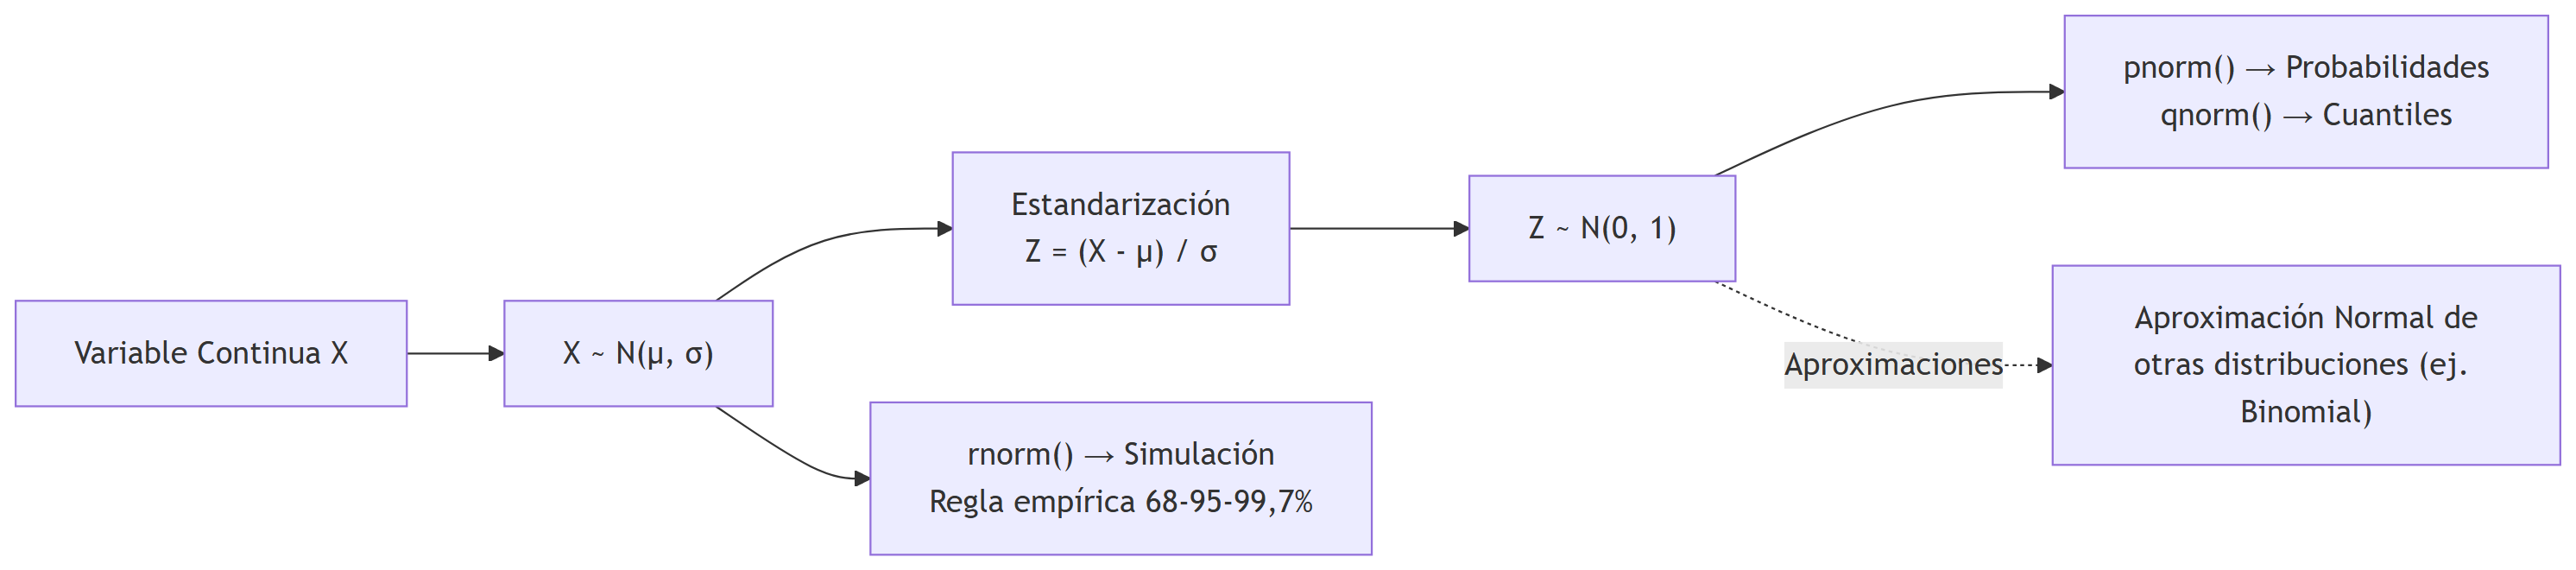
\includegraphics[width=13.74in,height=3.04in]{07_normal_files/figure-latex/mermaid-figure-1.png}

Marco conceptual de la Unidad de Distribución Normal

\section{\texorpdfstring{\textbf{Actividad de
pre-clase}}{Actividad de pre-clase}}\label{actividad-de-pre-clase-1}

Deberá copiar y pegar el siguiente \emph{prompt} dentro del chat del
cuaderno de \emph{Notebooklm}. Luego deberá copiar y pegar la respuesta
generada por la IA en un archivo .txt o bien en un documento de word o
similar.
\texttt{Se\ le\ solicitará\ la\ presentación\ del\ ejercicio\ durante\ la\ clase}.

\begin{Shaded}
\begin{Highlighting}[]

\NormalTok{Actúa como un asistente de Bioestadística de segundo año de la Licenciatura en Ciencias Biológicas. }
\NormalTok{La próxima clase veremos Distribución Normal o Gaussiana: propiedades, regla empírica, tipificación y cálculo de probabilidades.}

\NormalTok{Debes sugerirme UNA pregunta para hacerle al profesor al finalizar la clase. La pregunta debe:}
\NormalTok{{-} No ser una definición.}
\NormalTok{{-} Vincular el tema con un problema biológico real.}
\end{Highlighting}
\end{Shaded}

\textbf{Preguntas subidas al AV}

\emph{Comentarios generales}

Durante la clase hemos respondido brevemente algunos de los aportes que
han subido. A manera de síntesis, se observa que el cuaderno de géminis
les propone una pregunta que de alguna manera trata de resolver la
relación entre los datos empíricos (reales) y cuáles son las condiciones
y/o limitaciones de tratar de modelarlos suponiendo que fueron generados
por un proceso normal. Un aspecto que se repite con frecuencia en las
preguntas se relaciona con las variables que en la naturaleza sólo
pueden adoptar valores positivos, pero que al tratar de modelarlas por
medio de una distribución gaussiana, ésta podría asumir valores
negativos (por ejemplo, si el CV es elevado y \(\mu\) es próximo a 0.

Desde una perspectiva estadística, es necesario comprender los límites
de validez de la aproximación normal. En esos casos, la contribución del
análisis no consiste en descartar el modelo, sino en reconocer que la
normalidad es una aproximación útil en el centro de la distribución,
pero potencialmente poco representativa en los extremos de la
distribución. La aplicación de transformaciones de la variable para
aproximar a una distribución normal (por ejemplo la transformación
logarítmica) debe ser utilizada con cautela en determinadas
aplicaciones, se sugiere la lectura del ejemplo desarrollado sobre
análisis de materia orgánica en el predio de Severino, en la guía
Apuntes de Bioestadística con ejercicios resueltos.

Con respecto a la tipificación \(Z = \frac{X - \mu}{\sigma}\) y la regla
empírica (\(68\%,95\%,99,7\%\)), asumamos un grado aceptable de robustez
cuando el objetivo es estimar proporciones en la zona central de la
distribución (alrededor de la media), aun en presencia de asimetrías
moderadas. Pero si la asimetría observada en los datos es grande, las
estimaciones de probabilidad son poco confiables bajo el supuesto de
normalidad. Por el contrario, es posible presentar cuantiles en escala
tipificada aún para variables no normales, como una forma de simplificar
su lectura e interpretación. Se sugiere investigar acerca del Índice
Estandarizado de Precipitaciones (SPI), como un ejemplo de lo anterior.

\href{./ACTIVIDADES\%20CLASE/NORMAL/pre-clase_normal.txt}{Preguntas
generadas por la IA para este práctico (txt)}

\section{\texorpdfstring{\textbf{Actividad de
clase}}{Actividad de clase}}\label{actividad-de-clase-1}

\begin{itemize}
\item
  \textbf{Serena Chauque y Gianella Martínez} (Ejercicio 1)

  \begin{itemize}
  \tightlist
  \item
    \begin{enumerate}
    \def\labelenumi{\alph{enumi})}
    \tightlist
    \item
      Parámetros correctos; en sintaxis de R raramente usaremos las
      notaciones \(\mu\) y \(\sigma\), sino algo como
      \texttt{mu\ =\ 3.5}, \texttt{sigma\ =\ 0.6}.
    \end{enumerate}
  \item
    \begin{enumerate}
    \def\labelenumi{\alph{enumi})}
    \setcounter{enumi}{1}
    \tightlist
    \item
      \texttt{P(X\ ≤\ 2.8)\ =\ 0,1217} (correcto).
    \end{enumerate}
  \item
    \begin{enumerate}
    \def\labelenumi{\alph{enumi})}
    \setcounter{enumi}{2}
    \tightlist
    \item
      \texttt{P(X\ \textgreater{}\ 4.2)\ =\ 0,1217} (correcto; calculado
      mediante \texttt{1\ -\ pnorm(4.2,\ 3.5,\ 0.6)}).
    \end{enumerate}
  \item
    \begin{enumerate}
    \def\labelenumi{\alph{enumi})}
    \setcounter{enumi}{3}
    \tightlist
    \item
      \texttt{P(3.0\ ≤\ X\ ≤\ 4.0)\ =\ 0,5953} (correcto; resta de
      acumuladas
      \texttt{pnorm(4,\ 3.5,\ 0.6)\ -\ pnorm(3,\ 3.5,\ 0.6)}).
    \end{enumerate}
  \end{itemize}
\item
  \textbf{Baldo, Santiago; Muñoz, Paloma; Aramayo, Antonella} (Ejercicio
  1)

  \begin{itemize}
  \tightlist
  \item
    \begin{enumerate}
    \def\labelenumi{\alph{enumi})}
    \tightlist
    \item
      Parámetros correctos: \texttt{mu\ =\ 3.5}, \texttt{sigma\ =\ 0.6};
      en sintaxis de R raramente usaremos las notaciones \(\mu\) y
      \(\sigma\), sino algo como \texttt{mu\ =\ 3.5},
      \texttt{sigma\ =\ 0.6}.
    \end{enumerate}
  \item
    \begin{enumerate}
    \def\labelenumi{\alph{enumi})}
    \setcounter{enumi}{1}
    \tightlist
    \item
      \texttt{P(X\ ≤\ 2.8)\ =\ 0,1216} (12,16\%) (correcto, cuidado con
      los decimales, estrictamente el resultado se aproxima a 0,1217).
    \end{enumerate}
  \item
    \begin{enumerate}
    \def\labelenumi{\alph{enumi})}
    \setcounter{enumi}{2}
    \tightlist
    \item
      \texttt{P(X\ \textgreater{}\ 4.2)\ =\ 0,1216} (12,16\%) (correcto,
      cuidado con los decimales, estrictamente el resultado se aproxima
      a 0,1217).
    \end{enumerate}
  \item
    \begin{enumerate}
    \def\labelenumi{\alph{enumi})}
    \setcounter{enumi}{3}
    \tightlist
    \item
      \texttt{P(3.0\ ≤\ X\ ≤\ 4.0)\ =\ 0,5953} (59,53\%) (correcto).
    \end{enumerate}
  \end{itemize}
\item
  \textbf{Martínez, Julieta; Diaz, Candela} (Ejercicio 2)

  \begin{itemize}
  \tightlist
  \item
    \begin{enumerate}
    \def\labelenumi{\alph{enumi})}
    \tightlist
    \item
      \texttt{qnorm(0.10,\ 28.4,\ 3.2)\ =\ 24,2990} g/kg (correcto).
    \end{enumerate}
  \item
    \begin{enumerate}
    \def\labelenumi{\alph{enumi})}
    \setcounter{enumi}{1}
    \tightlist
    \item
      \texttt{qnorm(0.95,\ 28.4,\ 3.2)\ =\ 33,6635} g/kg (correcto).
    \end{enumerate}
  \item
    \begin{enumerate}
    \def\labelenumi{\alph{enumi})}
    \setcounter{enumi}{2}
    \tightlist
    \item
      Intervalo reportado \texttt{{[}24,29;\ 31,6{]}} (incorrecto). Para
      abarcar el 90\% simétrico central corresponde evaluar percentiles
      5 y 95: \texttt{qnorm(0.05,\ 28.4,\ 3.2)\ =\ 23,1365} y
      \texttt{qnorm(0.95,\ 28.4,\ 3.2)\ =\ 33,6635}. Intervalo correcto:
      \texttt{{[}23,14;\ 33,66{]}} g/kg.
    \end{enumerate}
  \item
    \begin{enumerate}
    \def\labelenumi{\alph{enumi})}
    \setcounter{enumi}{3}
    \tightlist
    \item
      Interpretación conceptual adecuada, sin embargo no es
      estrictamente necesario el empleo de valores estandarizados o
      tipificados.
    \end{enumerate}
  \end{itemize}
\item
  \textbf{Jimenez, Antonela; Garcia, Jimena; Lima, Abigail} (Ejercicio
  3)

  \begin{itemize}
  \tightlist
  \item
    \begin{enumerate}
    \def\labelenumi{\alph{enumi})}
    \tightlist
    \item
      Estandarización manual:
      \texttt{z\ =\ (45.0\ -\ 32.0)\ /\ 8.5\ =\ 1,5294} (correcto).
    \end{enumerate}
  \item
    \begin{enumerate}
    \def\labelenumi{\alph{enumi})}
    \setcounter{enumi}{1}
    \tightlist
    \item
      \texttt{P(Z\ ≤\ 1,5294)\ =\ 0,9369} (correcto).
    \end{enumerate}
  \item
    \begin{enumerate}
    \def\labelenumi{\alph{enumi})}
    \setcounter{enumi}{2}
    \tightlist
    \item
      Verificación en escala original:
      \texttt{pnorm(45,\ 32,\ 8.5)\ =\ 0,9369} (correcto).
    \end{enumerate}
  \item
    d)Faltó concluir sobre la posición del individuo dentro de la cola
    superior de la estructura del rodal.
  \end{itemize}
\item
  \textbf{Gonzalez, Arnaldo; Avendaño, Kyara; Vega, Leandro; Colodro,
  Silvia} (Ejercicio 3)

  \begin{itemize}
  \tightlist
  \item
    \begin{enumerate}
    \def\labelenumi{\alph{enumi})}
    \tightlist
    \item
      Estandarización manual:
      \texttt{z\ =\ (45.0\ -\ 32.0)\ /\ 8.5\ =\ 1,5294} (correcto).
    \end{enumerate}
  \item
    \begin{enumerate}
    \def\labelenumi{\alph{enumi})}
    \setcounter{enumi}{1}
    \tightlist
    \item
      \texttt{P(Z\ ≤\ 1,5294)\ =\ 0,9368} (93,68\%) (correcto).
    \end{enumerate}
  \item
    \begin{enumerate}
    \def\labelenumi{\alph{enumi})}
    \setcounter{enumi}{2}
    \tightlist
    \item
      Verificación directa: \texttt{pnorm(45,\ 32,\ 8.5)\ =\ 0,9368}
      (correcto).
    \end{enumerate}
  \item
    \begin{enumerate}
    \def\labelenumi{\alph{enumi})}
    \setcounter{enumi}{3}
    \tightlist
    \item
      Está bien la interpretación, faltaría ajustarla. El individuo
      estudiado presenta una DAP elevado en relación a la distribución
      de la población, tanto que se estima en casi un 94\% el porcentaje
      de individuos con DAP por debajo de 45 cm.
    \end{enumerate}
  \end{itemize}
\item
  \textbf{Ritu, Irina; Balanza Almada, Iara; Gutierrez Cortez, Casandra}
  (Ejercicio B4)

  \begin{itemize}
  \tightlist
  \item
    \begin{enumerate}
    \def\labelenumi{\alph{enumi})}
    \tightlist
    \item
      Sintaxis: \texttt{rnorm(60,\ 65.0,\ 11.2)} (correcto).
    \end{enumerate}
  \item
    \begin{enumerate}
    \def\labelenumi{\alph{enumi})}
    \setcounter{enumi}{1}
    \tightlist
    \item
      Estadísticos muestrales simulados: media = \texttt{65,73} g,
      desvío estándar = \texttt{10,19} g (correctos, son valores
      plausibles en la distribución).
    \end{enumerate}
  \item
    \begin{enumerate}
    \def\labelenumi{\alph{enumi})}
    \setcounter{enumi}{2}
    \tightlist
    \item
      Proporción empírica informada \texttt{\textless{}\ 50} g:
      \texttt{0,05} (5\%) (faltaría indicar cómo llegaron a esa
      estimación).
    \end{enumerate}
  \item
    \begin{enumerate}
    \def\labelenumi{\alph{enumi})}
    \setcounter{enumi}{3}
    \tightlist
    \item
      Probabilidad teórica:
      \texttt{P(X\ ≤\ 50)\ =\ pnorm(50,\ 65,\ 11.2)\ =\ 0,0902} (9,02\%)
      (correcto).
    \end{enumerate}
  \end{itemize}
\end{itemize}

\textbf{Producciones}

\href{./ACTIVIDADES\%20CLASE/NORMAL/normal.pdf}{Producciones de la
comisión del martes (PDF)}

\href{./ACTIVIDADES\%20CLASE/NORMAL/normal2.pdf}{Producciones de la
comisión del viernes (PDF)}

\section{Micro-ejercicios de aplicación
(optativos)}\label{micro-ejercicios-de-aplicaciuxf3n-optativos-4}

Los siguientes micro-ejercicios te permitirán practicar los conceptos
revisados en esta unidad. Puedes copiar y pegar las preguntas en un
script de R local, o bien utilizar \texttt{webR}, que es la versión
\emph{online} de R, disponible en esta guía.

\texttt{Nota}: los ejercicios están inspirados en trabajos científicos
publicados, pero contienen datos simulados. Por lo tanto, los resultados
obtenidos deben interpretarse únicamente con fines didácticos y no como
evidencia científica.

La finalidad es familiarizarse con el análisis estadístico y con el uso
de R a partir de situaciones similares a las que pueden encontrarse en
investigaciones reales.

\begin{Shaded}
\begin{Highlighting}[]

\CommentTok{\# =============================================================================}
\CommentTok{\#  Bioestadística — Facultad de Ciencias Agrarias {-} UNJu — Año 2026}
\CommentTok{\#  Ejercicios Optativos: Distribución Normal o Gaussiana}
\CommentTok{\# =============================================================================}
\CommentTok{\#}
\CommentTok{\#  Instrucciones generales}
\CommentTok{\#  {-}{-}{-}{-}{-}{-}{-}{-}{-}{-}{-}{-}{-}{-}{-}{-}{-}{-}{-}{-}{-}{-}{-}}
\CommentTok{\#  En cada ejercicio:}
\CommentTok{\#    (a) identifique la variable aleatoria, sus unidades y los parámetros (μ, σ)}
\CommentTok{\#    (b) plantee el cálculo de probabilidad o cuantil en notación estadística}
\CommentTok{\#    (c) realice la estandarización Z cuando corresponda y seleccione la función de R adecuada (pnorm, qnorm, rnorm, dnorm)}
\CommentTok{\#    (d) interprete la probabilidad calculada, el cuantil o los parámetros en el contexto biológico}
\CommentTok{\#    (e) elabore una conclusión o síntesis en el contexto del problema biológico}
\CommentTok{\#}
\CommentTok{\# =============================================================================}

\CommentTok{\#  Funciones disponibles (R base):}
\CommentTok{\#}
\CommentTok{\#    pnorm(q, mean = 0, sd = 1, lower.tail = TRUE)  \# Calcula probabilidad acumulada P(X \textless{}= q)}
\CommentTok{\#    qnorm(p, mean = 0, sd = 1, lower.tail = TRUE)  \# Calcula cuantil x\_p correspondiente a probabilidad p}
\CommentTok{\#    rnorm(n, mean = 0, sd = 1)                     \# Genera n observaciones aleatorias normales}
\CommentTok{\#    dnorm(x, mean = 0, sd = 1)                     \# Evalúa función de densidad de probabilidad f(x)}
\CommentTok{\#}
\CommentTok{\#  Estadísticos y fórmulas "manuales":}
\CommentTok{\#    Estandarización Z:            z = (x {-} mu) / sigma}
\CommentTok{\#    Estandarización inversa:         x = mu + z * sigma}
\CommentTok{\#    Regla Empírica:               mu +/{-} 1*sigma (\textasciitilde{}68\%), mu +/{-} 2*sigma (\textasciitilde{}95\%), mu +/{-} 3*sigma (\textasciitilde{}99.7\%)}
\CommentTok{\#    Aproximación Normal{-}Binomial: mu = n * p, sigma = sqrt(n * p * (1 {-} p))}
\CommentTok{\#}
\CommentTok{\# =============================================================================}


\CommentTok{\# ─────────────────────────────────────────────────────────────────────────────}
\CommentTok{\#  SECCIÓN 1 — PROBABILIDADES ACUMULADAS Y DE INTERVALO}
\CommentTok{\# ─────────────────────────────────────────────────────────────────────────────}

\CommentTok{\# Ejercicio N1}
\CommentTok{\# {-}{-}{-}{-}{-}{-}{-}{-}{-}{-}{-}{-}}
\CommentTok{\# En investigaciones sobre regeneración natural de bosques secos en la Quebrada}
\CommentTok{\# de Humahuaca (Jujuy), se estudia la morfometría de vainas de Algarrobo Blanco}
\CommentTok{\# (Prosopis alba). Registros biométricos indican que la longitud de las vainas (cm)}
\CommentTok{\# se distribuye normalmente con media μ = 16.2 cm y desvío estándar σ = 2.4 cm.}
\CommentTok{\#}
\CommentTok{\#  X: Longitud de la vaina de Prosopis alba (cm)}
\CommentTok{\#  X \textasciitilde{} N(μ = 16.2, σ = 2.4)}
\CommentTok{\#}
\CommentTok{\# a) Identifique la variable aleatoria, sus unidades e ingrese los}
\CommentTok{\#    parámetros μ y σ en objetos de R.}
\CommentTok{\# b) ¿Cuál es la probabilidad de que una vaina seleccionada al azar presente}
\CommentTok{\#    una longitud menor o igual a 13.5 cm?}
\CommentTok{\# c) ¿Cuál es la probabilidad de encontrar una vaina con una longitud superior}
\CommentTok{\#    a 19.0 cm?}
\CommentTok{\# d) ¿Cuál es la probabilidad de que la longitud de una vaina se encuentre entre}
\CommentTok{\#    14.0 cm y 18.0 cm?}
\CommentTok{\# e) En un lote muestral de N = 120 vainas colectadas en campo, ¿cuántas vainas}
\CommentTok{\#    se espera que tengan una longitud comprendida entre 14.0 cm y 18.0 cm?}

\CommentTok{\# Su código aquí:}


\CommentTok{\# Ejercicio N2}
\CommentTok{\# {-}{-}{-}{-}{-}{-}{-}{-}{-}{-}{-}{-}}
\CommentTok{\# En ensayos de caracterización ecofisiológica de ecotipos de Papa Andina}
\CommentTok{\# (Solanum tuberosum subsp. andigenum) en Tilcara, se mide la concentración de}
\CommentTok{\# clorofila foliar (unidades SPAD) mediante clorofilómetro óptico. Se asume que}
\CommentTok{\# la variable sigue una distribución normal con μ = 42.5 SPAD y σ = 5.2 SPAD.}
\CommentTok{\#}
\CommentTok{\#  X: Contenido de clorofila foliar en Papa Andina (SPAD)}
\CommentTok{\#  X \textasciitilde{} N(μ = 42.5, σ = 5.2)}
\CommentTok{\#}
\CommentTok{\# a) Defina la variable en R y configure el modelo probabilístico.}
\CommentTok{\# b) Plantee y calcule la probabilidad de que una planta presente un nivel de}
\CommentTok{\#    clorofila menor o igual a 35.0 SPAD (indicativo de deficiencia de nitrógeno).}
\CommentTok{\# c) Determine la probabilidad de que una planta supere los 50.0 SPAD de clorofila.}
\CommentTok{\# d) Sobre un total de N = 80 plantas evaluadas en la parcela experimental,}
\CommentTok{\#    ¿cuántas se espera que manifiesten deficiencia foliar (\textless{}= 35.0 SPAD)?}
\CommentTok{\# e) Elabore una síntesis sobre el impacto de estas probabilidades en la}
\CommentTok{\#    evaluación del estado nutricional del cultivo.}

\CommentTok{\# Su código aquí:}


\CommentTok{\# ─────────────────────────────────────────────────────────────────────────────}
\CommentTok{\#  SECCIÓN 2 — CUANTILES, PERCENTILES Y UMBRALES DE CRITERIO}
\CommentTok{\# ─────────────────────────────────────────────────────────────────────────────}

\CommentTok{\# Ejercicio N3}
\CommentTok{\# {-}{-}{-}{-}{-}{-}{-}{-}{-}{-}{-}{-}}
\CommentTok{\# En monitoreos herpetológicos en humedales de alta montaña en la Puna jujeña,}
\CommentTok{\# se evalúa la biomasa corporal (g) de renacuajos del Sapo Andino (Rhinella}
\CommentTok{\# spinulosa) en estadios larvales avanzados. Se estableció que el peso sigue}
\CommentTok{\# una distribución normal con media μ = 3.8 g y desvío estándar σ = 0.75 g.}
\CommentTok{\#}
\CommentTok{\#  X: Peso corporal de renacuajos de Rhinella spinulosa (g)}
\CommentTok{\#  X \textasciitilde{} N(μ = 3.8, σ = 0.75)}
\CommentTok{\#}
\CommentTok{\# a) Ingrese los parámetros de la distribución en objetos de R.}
\CommentTok{\# b) Mediante la función qnorm(), determine el peso máximo por debajo del cual}
\CommentTok{\#    se ubica el 15\% de los renacuajos con menor masa corporal (Percentil 15).}
\CommentTok{\# c) Calcule el umbral de peso por encima del cual se encuentra el 10\% de los}
\CommentTok{\#    individuos más desarrollados (Percentil 90).}
\CommentTok{\# d) Obtenga los límites del intervalo simétrico central que contiene al 80\% de}
\CommentTok{\#    la población de renacuajos en la cuenca.}
\CommentTok{\# e) Interprete biológicamente la utilidad de estos cuantiles para la detección}
\CommentTok{\#    de alertas por degradación del ecosistema acuático.}

\CommentTok{\# Su código aquí:}


\CommentTok{\# Ejercicio N4}
\CommentTok{\# {-}{-}{-}{-}{-}{-}{-}{-}{-}{-}{-}{-}}
\CommentTok{\# En estudios del ciclo de carbono y respiración edáfica en la Selva Pedemontana}
\CommentTok{\# del Parque Nacional Calilegua, se mide el flujo de emisión de CO2 del suelo}
\CommentTok{\# (μmol CO2 / m² s). Datos históricos muestran que la respiración del suelo}
\CommentTok{\# presenta una distribución normal con μ = 4.60 μmol CO2 / m² s y σ = 0.85 μmol CO2 / m² s.}
\CommentTok{\#}
\CommentTok{\#  X: Tasa de respiración edáfica (μmol CO2 / m² s)}
\CommentTok{\#  X \textasciitilde{} N(μ = 4.60, σ = 0.85)}
\CommentTok{\#}
\CommentTok{\# a) Cargue los parámetros en objetos de R.}
\CommentTok{\# b) Determine el primer cuartil (Q1 o Percentil 25) del flujo de CO2.}
\CommentTok{\# c) Verifique que el segundo cuartil (Q2 o Mediana) coincide exactamente con}
\CommentTok{\#    la media poblacional μ = 4.60 μmol CO2 / m² s.}
\CommentTok{\# d) Obtenga el cuantil del 95\% (Percentil 95) para la emisión respiratoria.}
\CommentTok{\# e) Discuta la relevancia de los cuantiles para caracterizar la variabilidad de}
\CommentTok{\#    la actividad biológica en suelos forestales de Yungas.}

\CommentTok{\# Su código aquí:}


\CommentTok{\# ─────────────────────────────────────────────────────────────────────────────}
\CommentTok{\#  SECCIÓN 3 — ESTANDARIZACIÓN Z, REGLA EMPÍRICA Y PROPIEDADES DE LA NORMAL}
\CommentTok{\# ─────────────────────────────────────────────────────────────────────────────}

\CommentTok{\# Ejercicio N5}
\CommentTok{\# {-}{-}{-}{-}{-}{-}{-}{-}{-}{-}{-}{-}}
\CommentTok{\# En investigaciones ecofisiológicas y conservación de avifauna amenazada en las}
\CommentTok{\# Serranías de Zenta (Jujuy), se mide la envergadura alar (cm) de machos adultos}
\CommentTok{\# de Cóndor Andino (Vultur gryphus). La variable sigue una distribución normal}
\CommentTok{\# con μ = 295.0 cm y σ = 12.0 cm. En una jornada de captura temporal para colocar}
\CommentTok{\# un emisor satelital, se registró un individuo con una envergadura x = 318.0 cm.}
\CommentTok{\#}
\CommentTok{\#  X: Envergadura alar en machos de Vultur gryphus (cm)}
\CommentTok{\#  X \textasciitilde{} N(μ = 295.0, σ = 12.0)}
\CommentTok{\#}
\CommentTok{\# a) Cargue en objetos de R los parámetros μ, σ y el valor observado x = 318.0.}
\CommentTok{\# b) Realice la estandarización manual calculando el estadístico z = (x {-} mu) / sigma}
\CommentTok{\#    e interprete el valor obtenido en términos de desvíos estándar.}
\CommentTok{\# c) Calcule la probabilidad acumulada P(Z \textless{}= z) sobre la variable tipificada N(0,1)}
\CommentTok{\#    utilizando la función pnorm(z).}
\CommentTok{\# d) Verifique la equivalencia probabilística calculando P(X \textless{}= 318.0) en la escala}
\CommentTok{\#    original mediante pnorm(318.0, mean = mu, sd = sigma).}
\CommentTok{\# e) Calcule P(X \textgreater{} 318.0) y concluya sobre la posición morfológica relativa de}
\CommentTok{\#    este ejemplar dentro de la población.}

\CommentTok{\# Su código aquí:}


\CommentTok{\# Ejercicio N6}
\CommentTok{\# {-}{-}{-}{-}{-}{-}{-}{-}{-}{-}{-}{-}}
\CommentTok{\# En un vivero forestal, se monitorea el crecimiento en altura (cm)}
\CommentTok{\# de plántulas de 1 año de Cedro Coya (Cedrela lilloi) para programas de enriquecimiento.}
\CommentTok{\# La altura se distribuye normalmente con media μ = 58.0 cm y desvío estándar σ = 7.5 cm.}
\CommentTok{\#}
\CommentTok{\#  X: Altura total de plántulas de Cedrela lilloi (cm)}
\CommentTok{\#  X \textasciitilde{} N(μ = 58.0, σ = 7.5)}
\CommentTok{\#}
\CommentTok{\# a) Ingrese los parámetros en objetos de R.}
\CommentTok{\# b) Mediante la regla empírica (mu +/{-} 1*sigma, mu +/{-} 2*sigma, mu +/{-} 3*sigma),}
\CommentTok{\#    calcule los rangos de altura que contienen aproximadamente al 68\%, 95\% y}
\CommentTok{\#    99.7\% central de las plántulas.}
\CommentTok{\# c) Compruebe las probabilidades teóricas exactas para cada intervalo utilizando}
\CommentTok{\#    la función pnorm().}
\CommentTok{\# d) Si un lote consta de N = 500 plántulas, ¿cuántas se espera que midan entre}
\CommentTok{\#    43.0 cm y 73.0 cm (intervalo de mu +/{-} 2*sigma)?}
\CommentTok{\# e) Redacte una síntesis sobre el uso de la regla empírica para la rápida inspección}
\CommentTok{\#    de calidad en viveros forestales.}

\CommentTok{\# Su código aquí:}


\CommentTok{\# Ejercicio N7}
\CommentTok{\# {-}{-}{-}{-}{-}{-}{-}{-}{-}{-}{-}{-}}
\CommentTok{\# En estudios de fisiología adaptativa en mamíferos de alta montaña, se examina}
\CommentTok{\# la frecuencia cardíaca en reposo (latidos/minuto) de hembras de Taruca}
\CommentTok{\# (Hippocamelus antisensis). La variable se distribuye normalmente con media}
\CommentTok{\# μ = 62.0 lat/min y desvío estándar σ = 6.0 lat/min.}
\CommentTok{\#}
\CommentTok{\#  X: Frecuencia cardíaca en reposo de Hippocamelus antisensis (lat/min)}
\CommentTok{\#  X \textasciitilde{} N(μ = 62.0, σ = 6.0)}
\CommentTok{\#}
\CommentTok{\# a) Defina los parámetros poblacionales en R.}
\CommentTok{\# b) Para una hembra con x = 74.0 lat/min, calcule el valor Z estandarizado y la}
\CommentTok{\#    probabilidad de registrar una frecuencia cardíaca aún mayor (P(X \textgreater{} 74.0)).}
\CommentTok{\# c) Determine mediante qnorm() los límites exactos del intervalo simétrico}
\CommentTok{\#    central que abarca el 95\% de las frecuencias cardíacas de la población.}
\CommentTok{\# d) Compare el intervalo simétrico exacto obtenido en c) con la aproximación de}
\CommentTok{\#    la regla empírica (mu +/{-} 2*sigma).}
\CommentTok{\# e) Comente la importancia ecofisiológica del control de la frecuencia cardíaca}
\CommentTok{\#    como indicador de estrés ambiental en la fauna autóctona.}

\CommentTok{\# Su código aquí:}


\CommentTok{\# ─────────────────────────────────────────────────────────────────────────────}
\CommentTok{\#  SECCIÓN 4 — SIMULACIÓN MUESTRAL Y APROXIMACIÓN NORMAL DE LA BINOMIAL}
\CommentTok{\# ─────────────────────────────────────────────────────────────────────────────}

\CommentTok{\# Ejercicio N8}
\CommentTok{\# {-}{-}{-}{-}{-}{-}{-}{-}{-}{-}{-}{-}}
\CommentTok{\# En investigaciones sobre frutales nativos en la localidad de Yala, se estudia}
\CommentTok{\# el peso de fruto fresco (g) en colectas de Tomate de Árbol (Solanum betaceum).}
\CommentTok{\# El peso sigue una distribución normal N(μ = 82.0, σ = 9.5).}
\CommentTok{\#}
\CommentTok{\#  X: Peso del fruto fresco de Solanum betaceum (g)}
\CommentTok{\#  X \textasciitilde{} N(μ = 82.0, σ = 9.5)}
\CommentTok{\#}
\CommentTok{\# a) Fije la semilla aleatoria con set.seed(123) y genere una muestra simulada}
\CommentTok{\#    de n = 100 frutos utilizando la función rnorm().}
\CommentTok{\# b) Calcule la media muestral y el desvío estándar muestral de los datos simulados}
\CommentTok{\#    utilizando mean() y sd(), y compárelos con los parámetros teóricos.}
\CommentTok{\# c) Determine la proporción empírica de frutos simulados que presentaron un}
\CommentTok{\#    peso menor o igual a 70.0 g.}
\CommentTok{\# d) Calcule la probabilidad teórica exacta P(X \textless{}= 70.0) mediante pnorm().}
\CommentTok{\# e) Evalúe el grado de coincidencia entre la proporción empírica obtenida en la}
\CommentTok{\#    simulación y el valor teórico esperado.}

\CommentTok{\# Su código aquí:}


\CommentTok{\# Ejercicio N9}
\CommentTok{\# {-}{-}{-}{-}{-}{-}{-}{-}{-}{-}{-}{-}}
\CommentTok{\# En estudios de dinámica poblacional e ictiología en la cuenca del Río San}
\CommentTok{\# Francisco (Jujuy), se evalúa la longitud estándar (cm) de juveniles de Sábalo}
\CommentTok{\# (Prochilodus lineatus). Se asume una distribución normal N(μ = 24.5, σ = 3.2).}
\CommentTok{\#}
\CommentTok{\#  X: Longitud estándar de juveniles de Prochilodus lineatus (cm)}
\CommentTok{\#  X \textasciitilde{} N(μ = 24.5, σ = 3.2)}
\CommentTok{\#}
\CommentTok{\# a) Simule una muestra de n = 1000 peces utilizando rnorm() para representar un}
\CommentTok{\#    muestreo biológico en época de cardumen.}
\CommentTok{\# b) Obtenga la media y el desvío estándar de la muestra generada.}
\CommentTok{\# c) Determine la proporción empírica de ejemplares que superan los 30.0 cm de}
\CommentTok{\#    longitud (talla mínima para un ensayo experimental de captura).}
\CommentTok{\# d) Compare la proporción empírica con la probabilidad teórica P(X \textgreater{} 30.0)}
\CommentTok{\#    calculada con pnorm().}
\CommentTok{\# e) Concluya sobre la utilidad de las simulaciones Monte Carlo para el diseño}
\CommentTok{\#    de planes de manejo pesquero y fiscalización ambiental.}

\CommentTok{\# Su código aquí:}


\CommentTok{\# Ejercicio N10}
\CommentTok{\# {-}{-}{-}{-}{-}{-}{-}{-}{-}{-}{-}{-}{-}}
\CommentTok{\# En evaluaciones de fitopatología agrícola en la Quebrada de Humahuaca, se}
\CommentTok{\# analiza la prevalencia de mildiu (Peronospora variabilis) en plantas de Quinoa.}
\CommentTok{\# La probabilidad individual de infección en una planta es p = 0.28. Un técnico}
\CommentTok{\# agrónomo inspecciona una muestra de n = 50 plantas independientes en un lote.}
\CommentTok{\#}
\CommentTok{\#  Variable original: X \textasciitilde{} Binomial(n = 50, p = 0.28)}
\CommentTok{\#}
\CommentTok{\# a) Verifique el cumplimiento de los requisitos para aplicar la aproximación}
\CommentTok{\#    Normal a la Binomial (n * p \textgreater{} 5 y n * (1 {-} p) \textgreater{} 5).}
\CommentTok{\# b) Calcule los parámetros de la distribución Normal aproximada:}
\CommentTok{\#    μ = n * p   y   σ = sqrt(n * p * (1 {-} p)).}
\CommentTok{\# c) Utilizando la aproximación Normal con corrección por continuidad (+0.5),}
\CommentTok{\#    calcule la probabilidad de que a lo sumo 18 plantas estén infectadas}
\CommentTok{\#    P(X \textless{}= 18) ≈ P(X\textquotesingle{} \textless{}= 18.5) mediante la función pnorm().}
\CommentTok{\# d) Si se inspeccionan N = 120 parcelas similares de n = 50 plantas cada una,}
\CommentTok{\#    ¿en cuántas parcelas se espera encontrar como máximo 18 plantas infectadas?}
\CommentTok{\# e) Elabore una síntesis comparativa sobre la ventaja analítica y computacional}
\CommentTok{\#    de emplear la aproximación Normal cuando el tamaño muestral es mediano a grande.}

\CommentTok{\# Su código aquí:}


\CommentTok{\# =============================================================================}
\end{Highlighting}
\end{Shaded}

\bookmarksetup{startatroot}

\chapter*{Primer Parcial \textbar{} 2026}\label{primer-parcial-2026}
\addcontentsline{toc}{chapter}{Primer Parcial \textbar{} 2026}

\markboth{Primer Parcial \textbar{} 2026}{Primer Parcial \textbar{}
2026}

El primer \texttt{parcial\ de\ Bioestadística\ 2026} tendrá lugar
durante la semana del 21 al 25 de septiembre de 2026:
\texttt{Martes\ 22/09\ de\ 14.00\ a\ 16.00\ (Comisión\ de\ la\ tarde)},
y
\texttt{viernes\ 25/09\ de\ 10.15\ a\ 12.15\ (Comisión\ de\ la\ mañana)},
en el \textbf{Aula 3A}.

\begin{tcolorbox}[enhanced jigsaw, arc=.35mm, bottomrule=.15mm, bottomtitle=1mm, breakable, colback=white, colbacktitle=quarto-callout-important-color!10!white, colframe=quarto-callout-important-color-frame, coltitle=black, left=2mm, leftrule=.75mm, opacityback=0, opacitybacktitle=0.6, rightrule=.15mm, title=\textcolor{quarto-callout-important-color}{\faExclamation}\hspace{0.5em}{Pautas}, titlerule=0mm, toprule=.15mm, toptitle=1mm]

\begin{itemize}
\item
  El parcial será \textbf{presencial,} y podrá ser realizado en grupos
  de hasta \textbf{2 (dos) personas}. Deberán contar con una computadora
  ya que deberán realizar cálculos estadísticos (tomar las previsiones
  con tiempo, \emph{como tener cargada la computadora, o bien traer
  zapatilla}).
\item
  Al ingresar al Aula, \textbf{deberán dejar sus celulares en un
  recipiente que se les proporcionará.} No necesitarán conexión a
  internet para poder resolver el cuestionario. No obstante, la
  resolución será a ``libro abierto'', por lo que les resultará de
  utilidad conformar un ``script madre'' donde anoten todas las
  funciones que hayan utilizado en las actividades de entrenamiento,
  para utilizarlas durante el parcial.
\item
  El formato de entrega será \textbf{escrito, y deberán colocar todas
  las respuestas en la hoja suministrada}. Además de la entrega, los
  parciales deberán \textbf{ser defendidos/validados en forma oral},
  para lo cual deberán acercarse a la cátedra hasta el día
  \textbf{viernes 09/10/2026}. Preferentemente en el horario de
  consulta, o bien coordinar con el profesor el horario para el resto de
  los días/horas de la semana.
\end{itemize}

\end{tcolorbox}

\begin{tcolorbox}[enhanced jigsaw, arc=.35mm, bottomrule=.15mm, bottomtitle=1mm, breakable, colback=white, colbacktitle=quarto-callout-tip-color!10!white, colframe=quarto-callout-tip-color-frame, coltitle=black, left=2mm, leftrule=.75mm, opacityback=0, opacitybacktitle=0.6, rightrule=.15mm, title=\textcolor{quarto-callout-tip-color}{\faLightbulb}\hspace{0.5em}{Clase de Consulta}, titlerule=0mm, toprule=.15mm, toptitle=1mm]

El día \textbf{jueves 10 de septiembre de 2026 de 14.00 a 16.00}
tendremos una clase de consulta, en forma virtual. Se compartirá enlace
a través del foro del Aula Virtual. Trabajaremos todos los temas vistos,
hasta distribuciones discretas.

No olviden completar \texttt{la\ encuesta\ de\ retroalimentación}
disponible en el Aula Virtual hasta el lunes 07/09, para poder organizar
mejor la clase de consulta.

\end{tcolorbox}

\section*{Resultados del primer
parcial}\label{resultados-del-primer-parcial}
\addcontentsline{toc}{section}{Resultados del primer parcial}

\markright{Resultados del primer parcial}

Se presentan las calificaciones obtenidas en el primer parcial de
Bioestadística 2026, en su formato escrito. Recuerden que los parciales
deberán \textbf{ser defendidos/validados en forma oral}, para lo cual
deberán acercarse a la cátedra hasta el día \textbf{viernes 09/10/2026}.
Preferentemente en el horario de consulta, o bien coordinar con el
profesor el horario para el resto de los días/horas de la semana.
\textbf{NOTA:} Los grupos que no alcanzaron la nota de promoción (7)
continúen cursando en modalidad promocional. Hacia el final de la
cursada se habilitará una instancia para recuperar los incisos no
aprobados, de forma tal que podrán aumentar la calificación. Los
cuestionarios prácticos correspondientes a la primera parte de la
cursada estarán habilitados hasta el 02/10/2026 para su resolución. En
caso de que algún cuestionario quede sin aprobar, deberán rehacer el
primer parcial.

\begin{table}
\centering
\caption{\label{tab:unnamed-chunk-2}Calificaciones del Primer Parcial de Bioestadística - FCA UNJu 2026}
\centering
\begin{tabular}[t]{l|c|>{}c}
\hline
\cellcolor[HTML]{D9E1F2}{\textbf{Apellido y Nombre}} & \cellcolor[HTML]{D9E1F2}{\textbf{Comisión}} & \cellcolor[HTML]{D9E1F2}{\textbf{Nota}}\\
\hline
Lima, Mariela; García, Jimena & 2 & \textbf{8.8}\\
\hline
Gutiérrez Cortez, Casandra; Ritú, Irina Leticia & 1 & \textbf{8.0}\\
\hline
Jiménez Serra, Antonella & 2 & \textbf{7.0}\\
\hline
Colodro, Silvia Verónica; Gómez, Benjamín Alejandro & 2 & \textbf{8.0}\\
\hline
Baldo, Santiago; Muñoz, Paloma & 1 & \textbf{9.6}\\
\hline
Balanza, Iara Guadalupe; Cruz, Rocío Belén & 1 & \textbf{9.5}\\
\hline
Aramayo, Antonella; Díaz, Candela & 1 & \textbf{6.0}\\
\hline
Avendaño, Kiara Celeste; Vega Villafañe, Leandro & 1 & \textbf{9.0}\\
\hline
González, Arnaldo; Chauque, Serena Josefina & 1 / 2 & \textbf{7.0}\\
\hline
Martínez, Gianella & 2 & \textbf{5.5}\\
\hline
\end{tabular}
\end{table}

\begin{itemize}
\tightlist
\item
  \href{./PRIMER\%20PARCIAL/RESOLUCIÓN\%20PARCIAL\%201.R}{PROPUESTA DE
  RESOLUCIÓN}
\item
  \href{./PRIMER\%20PARCIAL/anotaciones\%20primer\%20parcial\%202026.txt}{DEVOLUCIÓN}
\end{itemize}

\bookmarksetup{startatroot}

\chapter{Trabajo Práctico 5: Inferencia con Muestras
Grandes}\label{trabajo-pruxe1ctico-5-inferencia-con-muestras-grandes}

Objetivos del Trabajo Práctico El objetivo de esta unidad es que el
estudiante construya las bases de la inferencia estadística a partir de
muestras, comprendiendo el rol de la Ley de los Grandes Números y el
Teorema Central del Límite como fundamentos teóricos. A partir de ellos,
se busca que el estudiante sea capaz de: (1) Distinguir entre parámetros
poblacionales y estadísticos muestrales, y entender su relación; (2)
Utilizar estimadores puntuales y construir intervalos de confianza,
interpretando correctamente su significado; (3) Formular y evaluar
contrastes de hipótesis, incorporando los conceptos de nivel de
significación y error; (4) Justificar, en términos probabilísticos, el
uso de aproximaciones basadas en muestras grandes; y (5) Aplicar estos
procedimientos en diferentes situaciones, evaluando la validez de los
supuestos involucrados.

\begin{tcolorbox}[enhanced jigsaw, arc=.35mm, bottomrule=.15mm, bottomtitle=1mm, breakable, colback=white, colbacktitle=quarto-callout-important-color!10!white, colframe=quarto-callout-important-color-frame, coltitle=black, left=2mm, leftrule=.75mm, opacityback=0, opacitybacktitle=0.6, rightrule=.15mm, title=\textcolor{quarto-callout-important-color}{\faExclamation}\hspace{0.5em}{Lectura Sugerida para el Trabajo Práctico}, titlerule=0mm, toprule=.15mm, toptitle=1mm]

Se recomienda a los estudiantes consultar el libro \textbf{«Apuntes de
Bioestadística. Con ejercicios resueltos»} para profundizar los
conceptos teóricos y metodológicos desarrollados en este marco:

\begin{itemize}
\tightlist
\item
  \textbf{Unidad 7: Teorema Central del Límite y Ley de los Grandes
  Números}: Consultar las condiciones de aplicabilidad de ambos
  resultados, su interpretación, y el ajuste por corrección de población
  finita cuando la muestra representa una fracción no despreciable de la
  población.
\item
  \textbf{Unidad 7: Estimación Puntual, Intervalos de Confianza y Prueba
  de Hipótesis}: Revisar las propiedades de un buen estimador
  (insesgadez, error estándar), la construcción e interpretación de un
  intervalo de confianza, y los pasos de una prueba de hipótesis
  (planteo de hipótesis, nivel de significación, estadístico de prueba,
  regla de decisión, y los errores de Tipo I y Tipo II).
\end{itemize}

Como lecturas complementarias, se sugiere también revisar la unidad
\emph{«Estimación de Parámetros y Contraste de Hipótesis»} del libro
\textbf{«Estadística y Biometría»} de Balzarini et al.; la unidad
\emph{«Inference»} del libro \textbf{«Data Analysis for the Life
Sciences»} de Irizarry et al.; y las unidades \emph{«Testing
Hypotheses»} y \emph{«Goodness-of-Fit Test»} del libro
\textbf{«Biostatistics with R»} de Leps y Smilauer.

\end{tcolorbox}

\section{Generalidades}\label{generalidades-3}

En las unidades anteriores se trabajó con distribuciones de probabilidad
cuyos parámetros se asumían conocidos. En la práctica, muchas veces esos
parámetros poblacionales rara vez se conocen: lo habitual es contar
únicamente con una muestra, y a partir de ella inferir las
características de la población de la que proviene. La
\textbf{Estadística Inferencial} es la rama de la estadística que se
ocupa de estimar de forma inductiva características poblacionales
(parámetros) a partir de lo observado en una muestra probabilística
(estadísticos).

\subsection{Muestras grandes}\label{muestras-grandes}

El desarrollo de la inferencia a partir de muestras grandes se apoya en
dos postulados teóricos: La \textbf{Ley de los Grandes Números}
establece que, a medida que aumenta el tamaño de una muestra aleatoria,
el promedio muestral converge en probabilidad al verdadero valor del
parámetro poblacional que se busca estimar. Por su parte, el
\textbf{Teorema Central del Límite (TCL)} establece que, si el tamaño
muestral es suficientemente grande, la distribución del promedio
muestral se aproxima a una distribución Normal, independientemente de
cuál sea la distribución de la variable original. Ambos postulados
permiten construir procedimientos de inferencia válidos aun sin conocer
la distribución exacta de la variable en estudio, y son la razón por la
cual esta unidad requiere trabajar con muestras de tamaño grande.

\subsection{Parámetro, estadístico y
estimador}\label{paruxe1metro-estaduxedstico-y-estimador}

Para avanzar en la inferencia es necesario distinguir tres conceptos: Un
\textbf{parámetro} es una característica de la población (por ejemplo,
una media o una proporción poblacional) cuyo valor es constante pero, en
general, desconocido. Un \textbf{estadístico} es cualquier función
calculada a partir de una muestra aleatoria (por ejemplo, la media o la
proporción muestral). Cuando ese estadístico se utiliza para aproximar
el valor de un parámetro, se lo denomina \textbf{estimador} del mismo. A
partir de esta distinción, existen tres formas de abordar la estimación
de un parámetro: la \textbf{estimación puntual} (proponer un único valor
que lo aproxime), la \textbf{estimación por intervalo de confianza}
(proponer un rango de valores plausibles, asociado a un nivel de
confianza), y la \textbf{prueba de hipótesis} (contrastar formalmente
una conjetura sobre el parámetro frente a la evidencia muestral
disponible, controlando la probabilidad de los errores de Tipo I y Tipo
II).

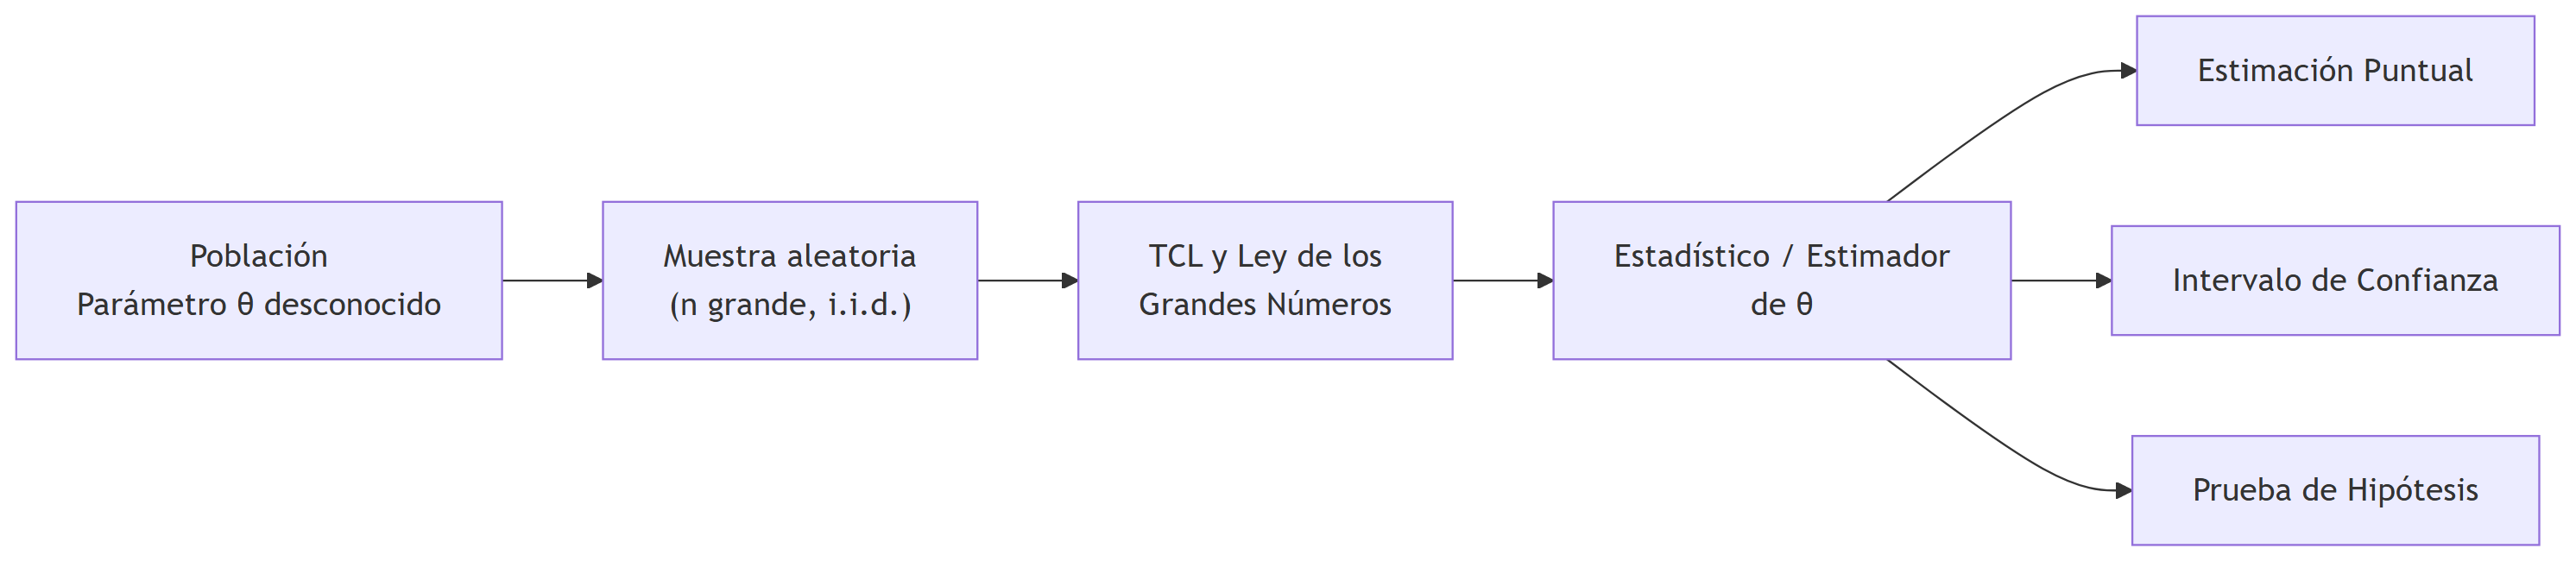
\includegraphics[width=13.29in,height=2.9in]{08_inferencia_muestras_grandes_files/figure-latex/mermaid-figure-1.png}

Marco conceptual de la Unidad de Inferencia con Muestras Grandes

\section{\texorpdfstring{\textbf{Actividad de
pre-clase}}{Actividad de pre-clase}}\label{actividad-de-pre-clase-2}

Deberá copiar y pegar el siguiente \emph{prompt} dentro del chat del
cuaderno de \emph{Notebooklm}. Luego deberá copiar y pegar la respuesta
generada por la IA en un archivo .txt o bien en un documento de word o
similar.
\texttt{Se\ le\ solicitará\ la\ presentación\ del\ ejercicio\ durante\ la\ clase}.

\begin{Shaded}
\begin{Highlighting}[]
\NormalTok{Actúa como un asistente de Bioestadística de segundo año de la Licenciatura en Ciencias Biológicas. }
\NormalTok{La próxima clase veremos Inferencia con muestras grandes}\SpecialCharTok{:} 
  \SpecialCharTok{{-}}\NormalTok{ Inferencia de la media poblacional con muestras grandes o cuando se conoce sigma}
  \SpecialCharTok{{-}}\NormalTok{ Inferencia de una proporción poblacional}
  \SpecialCharTok{{-}}\NormalTok{ Inferencia de la comparación de }\DecValTok{2}\NormalTok{ proporciones poblacionales.}
\NormalTok{Debes sugerirme UNA pregunta para hacerle al profesor al finalizar la clase. La pregunta debe}\SpecialCharTok{:}
\SpecialCharTok{{-}}\NormalTok{ No ser una definición.}
\SpecialCharTok{{-}}\NormalTok{ Vincular el tema con un problema biológico real.}
\NormalTok{Nota}\SpecialCharTok{:}\NormalTok{ No proponer una pregunta por tema, elegir un tema y sobre el mismo proponer una pregunta.}
\end{Highlighting}
\end{Shaded}

\section{Micro-ejercicios de aplicación
(optativos)}\label{micro-ejercicios-de-aplicaciuxf3n-optativos-5}

Los siguientes micro-ejercicios te permitirán practicar los conceptos
revisados en esta unidad. Puedes copiar y pegar las preguntas en un
script de R local, o bien utilizar \texttt{webR}, que es la versión
\emph{online} de R, disponible en esta guía.

\texttt{Nota}: los ejercicios están inspirados en trabajos científicos
publicados, pero contienen datos simulados. Por lo tanto, los resultados
obtenidos deben interpretarse únicamente con fines didácticos y no como
evidencia científica.

La finalidad es familiarizarse con el análisis estadístico y con el uso
de R a partir de situaciones similares a las que pueden encontrarse en
investigaciones reales.

\begin{Shaded}
\begin{Highlighting}[]

\CommentTok{\# =============================================================================}
\CommentTok{\# EJERCICIOS OPTATIVOS DE R: INFERENCIA ESTADISTICA EN MUESTRAS GRANDES}
\CommentTok{\# =============================================================================}
\CommentTok{\#}
\CommentTok{\# Este archivo contiene 15 ejercicios practicos divididos en 3 bloques}
\CommentTok{\# tematicos:}
\CommentTok{\#   {-} Bloque 1: Inferencia sobre la Media Poblacional (mu)              {-} 5 ejercicios}
\CommentTok{\#   {-} Bloque 2: Inferencia sobre una Proporcion Poblacional (p)         {-} 5 ejercicios}
\CommentTok{\#   {-} Bloque 3: Inferencia para Dos Proporciones Poblacionales (p1{-}p2)  {-} 5 ejercicios}
\CommentTok{\#}
\CommentTok{\# Cada ejercicio incluye contexto biologico, datos de entrada y consignas}
\CommentTok{\# especificas. Complete el codigo en R en los espacios indicados.}


\CommentTok{\# \#\#\#\#\#\#\#\#\#\#\#\#\#\#\#\#\#\#\#\#\#\#\#\#\#\#\#\#\#\#\#\#\#\#\#\#\#\#\#\#\#\#\#\#\#\#\#\#\#\#\#\#\#\#\#\#\#\#\#\#\#\#\#\#\#\#\#\#\#\#\#\#\#\#\#\#\#}
\CommentTok{\# BLOQUE 1: INFERENCIA SOBRE LA MEDIA POBLACIONAL (mu) CON MUESTRAS GRANDES}
\CommentTok{\# \#\#\#\#\#\#\#\#\#\#\#\#\#\#\#\#\#\#\#\#\#\#\#\#\#\#\#\#\#\#\#\#\#\#\#\#\#\#\#\#\#\#\#\#\#\#\#\#\#\#\#\#\#\#\#\#\#\#\#\#\#\#\#\#\#\#\#\#\#\#\#\#\#\#\#\#\#}

\CommentTok{\# {-}{-}{-}{-}{-}{-}{-}{-}{-}{-}{-}{-}{-}{-}{-}{-}{-}{-}{-}{-}{-}{-}{-}{-}{-}{-}{-}{-}{-}{-}{-}{-}{-}{-}{-}{-}{-}{-}{-}{-}{-}{-}{-}{-}{-}{-}{-}{-}{-}{-}{-}{-}{-}{-}{-}{-}{-}{-}{-}{-}{-}{-}{-}{-}{-}{-}{-}{-}{-}{-}{-}{-}{-}{-}{-}{-}{-}}
\CommentTok{\# EJERCICIO 1: Concentracion de Hemoglobina en Peces de un Rio Contaminado}
\CommentTok{\# {-}{-}{-}{-}{-}{-}{-}{-}{-}{-}{-}{-}{-}{-}{-}{-}{-}{-}{-}{-}{-}{-}{-}{-}{-}{-}{-}{-}{-}{-}{-}{-}{-}{-}{-}{-}{-}{-}{-}{-}{-}{-}{-}{-}{-}{-}{-}{-}{-}{-}{-}{-}{-}{-}{-}{-}{-}{-}{-}{-}{-}{-}{-}{-}{-}{-}{-}{-}{-}{-}{-}{-}{-}{-}{-}{-}{-}}

\CommentTok{\# Contexto:}
\CommentTok{\# Un equipo de ecotoxicologia evalua el impacto de efluentes industriales en}
\CommentTok{\# el bienestar fisiologico de una especie de pez nativo. }
\CommentTok{\# Se sabe que la concentracion media normal de hemoglobina en}
\CommentTok{\# aguas no contaminadas es de mu\_0 = 9.0 g/dL y sigma = 1.6 g/dL. Se toma una muestra aleatoria}
\CommentTok{\# de n = 120 peces en la zona afectada.}
\CommentTok{\#}
\CommentTok{\# Datos: n = 120, x\_barra = 8.4 g/dL, sigma = 1.6 g/dL, alpha = 0.05.}
\CommentTok{\#}
\CommentTok{\# Consignas:}
\CommentTok{\# 1. Construya un intervalo de confianza del 95\% para la concentracion}
\CommentTok{\#    media poblacional de hemoglobina (mu) en la zona afectada usando}
\CommentTok{\#    qnorm().}
\CommentTok{\# 2. Plantee y ejecute una prueba Z unilateral izquierda para determinar si}
\CommentTok{\#    la concentracion media es significativamente inferior a 9.0 g/dL.}
\CommentTok{\# 3. Calcule el valor p mediante pnorm() e indique la decision estadistica.}

\NormalTok{n }\OtherTok{=} \DecValTok{120}
\NormalTok{x\_bar }\OtherTok{=} \FloatTok{8.4}
\NormalTok{sigma }\OtherTok{=} \FloatTok{1.6}
\NormalTok{mu\_0 }\OtherTok{=} \FloatTok{9.0}
\NormalTok{alpha }\OtherTok{=} \FloatTok{0.05}

\CommentTok{\# 1. Intervalo de Confianza del 95\% para mu}
\CommentTok{\# Su código aquí:}



\CommentTok{\# 2 y 3. Estadístico Z, valor p y decisión (H0: mu \textgreater{}= 9.0 vs H1: mu \textless{} 9.0)}
\CommentTok{\# Su código aquí:}



\CommentTok{\# {-}{-}{-}{-}{-}{-}{-}{-}{-}{-}{-}{-}{-}{-}{-}{-}{-}{-}{-}{-}{-}{-}{-}{-}{-}{-}{-}{-}{-}{-}{-}{-}{-}{-}{-}{-}{-}{-}{-}{-}{-}{-}{-}{-}{-}{-}{-}{-}{-}{-}{-}{-}{-}{-}{-}{-}{-}{-}{-}{-}{-}{-}{-}{-}{-}{-}{-}{-}{-}{-}{-}{-}{-}{-}{-}{-}{-}}
\CommentTok{\# EJERCICIO 2: Biomasa Seca de Plantulas de Pinus taeda bajo Fertilizante Organomineral}
\CommentTok{\# {-}{-}{-}{-}{-}{-}{-}{-}{-}{-}{-}{-}{-}{-}{-}{-}{-}{-}{-}{-}{-}{-}{-}{-}{-}{-}{-}{-}{-}{-}{-}{-}{-}{-}{-}{-}{-}{-}{-}{-}{-}{-}{-}{-}{-}{-}{-}{-}{-}{-}{-}{-}{-}{-}{-}{-}{-}{-}{-}{-}{-}{-}{-}{-}{-}{-}{-}{-}{-}{-}{-}{-}{-}{-}{-}{-}{-}}

\CommentTok{\# Contexto:}
\CommentTok{\# En un ensayo silvicultural, se aplica un biofertilizante a n = 150}
\CommentTok{\# plantulas de Pinus taeda. Transcurridos 6 meses, se mide el peso seco de}
\CommentTok{\# la parte aerea (en gramos). Se obtiene una media muestral de}
\CommentTok{\# x\_barra = 14.8 g y s = 2.5 g.}
\CommentTok{\# Nota: aproxime s a sigma, por tamaño muestral.}
\CommentTok{\#}
\CommentTok{\# Datos: n = 150, x\_barra = 14.8 g, s = 2.5 g, nivel de confianza = 99\%.}
\CommentTok{\#}
\CommentTok{\# Consignas:}
\CommentTok{\# 1. Calcule el intervalo de confianza del 99\% para la biomasa seca}
\CommentTok{\#    promedio poblacional.}
\CommentTok{\# 2. ¿Qué tamaño muestral n se requeriría si se desea estimar la biomasa}
\CommentTok{\#    media con un margen de error máximo de E = 0.30 g al 99\% de}
\CommentTok{\#    confianza?}

\NormalTok{n }\OtherTok{=} \DecValTok{150}
\NormalTok{x\_bar }\OtherTok{=} \FloatTok{14.8}
\NormalTok{s }\OtherTok{=} \FloatTok{2.5}
\NormalTok{confianza }\OtherTok{=} \FloatTok{0.99}
\NormalTok{alpha }\OtherTok{=} \DecValTok{1} \SpecialCharTok{{-}}\NormalTok{ confianza}

\CommentTok{\# 1. Intervalo de Confianza del 99\%}
\CommentTok{\# Su código aquí:}



\CommentTok{\# 2. Tamaño Muestral Necesario para E = 0.30 g}
\NormalTok{E }\OtherTok{=} \FloatTok{0.30}
\CommentTok{\# Su código aquí:}



\CommentTok{\# {-}{-}{-}{-}{-}{-}{-}{-}{-}{-}{-}{-}{-}{-}{-}{-}{-}{-}{-}{-}{-}{-}{-}{-}{-}{-}{-}{-}{-}{-}{-}{-}{-}{-}{-}{-}{-}{-}{-}{-}{-}{-}{-}{-}{-}{-}{-}{-}{-}{-}{-}{-}{-}{-}{-}{-}{-}{-}{-}{-}{-}{-}{-}{-}{-}{-}{-}{-}{-}{-}{-}{-}{-}{-}{-}{-}{-}}
\CommentTok{\# EJERCICIO 3: Tasa Metabolica Basal en Roedores Silvestres (Akodon azarae)}
\CommentTok{\# {-}{-}{-}{-}{-}{-}{-}{-}{-}{-}{-}{-}{-}{-}{-}{-}{-}{-}{-}{-}{-}{-}{-}{-}{-}{-}{-}{-}{-}{-}{-}{-}{-}{-}{-}{-}{-}{-}{-}{-}{-}{-}{-}{-}{-}{-}{-}{-}{-}{-}{-}{-}{-}{-}{-}{-}{-}{-}{-}{-}{-}{-}{-}{-}{-}{-}{-}{-}{-}{-}{-}{-}{-}{-}{-}{-}{-}}

\CommentTok{\# Contexto:}
\CommentTok{\# Un ecofisiologo evalua el consumo de oxigeno en reposo (mL O2 / g*h) en}
\CommentTok{\# una poblacion silvestre de Akodon azarae en invierno. El valor de}
\CommentTok{\# referencia historico de primavera es mu\_0 = 2.00 mL O2 / g*h y sigma = 0.42 mL O2 / g*h. Se captura}
\CommentTok{\# y mide a n = 100 individuos.}
\CommentTok{\#}
\CommentTok{\# Datos: n = 100, x\_barra = 2.15, sigma = 0.42, mu\_0 = 2.00, alpha = 0.01.}
\CommentTok{\#}
\CommentTok{\# Consignas:}
\CommentTok{\# 1. Realice una prueba Z bilateral para determinar si la tasa metabolica}
\CommentTok{\#    difiere del valor de primavera.}
\CommentTok{\# 2. Calcule el valor p exacto empleando pnorm() e interprete la decision a}
\CommentTok{\#    un nivel alpha = 0.01.}

\NormalTok{n }\OtherTok{=} \DecValTok{100}
\NormalTok{x\_bar }\OtherTok{=} \FloatTok{2.15}
\NormalTok{sigma }\OtherTok{=} \FloatTok{0.42}
\NormalTok{mu\_0 }\OtherTok{=} \FloatTok{2.00}
\NormalTok{alpha }\OtherTok{=} \FloatTok{0.01}

\CommentTok{\# 1 y 2. Estadístico Z, valor p bilateral y decisión}
\CommentTok{\# Su código aquí:}



\CommentTok{\# {-}{-}{-}{-}{-}{-}{-}{-}{-}{-}{-}{-}{-}{-}{-}{-}{-}{-}{-}{-}{-}{-}{-}{-}{-}{-}{-}{-}{-}{-}{-}{-}{-}{-}{-}{-}{-}{-}{-}{-}{-}{-}{-}{-}{-}{-}{-}{-}{-}{-}{-}{-}{-}{-}{-}{-}{-}{-}{-}{-}{-}{-}{-}{-}{-}{-}{-}{-}{-}{-}{-}{-}{-}{-}{-}{-}{-}}
\CommentTok{\# EJERCICIO 4: Longitud Corporal de una Poblacion de Anuros Amenazados}
\CommentTok{\# {-}{-}{-}{-}{-}{-}{-}{-}{-}{-}{-}{-}{-}{-}{-}{-}{-}{-}{-}{-}{-}{-}{-}{-}{-}{-}{-}{-}{-}{-}{-}{-}{-}{-}{-}{-}{-}{-}{-}{-}{-}{-}{-}{-}{-}{-}{-}{-}{-}{-}{-}{-}{-}{-}{-}{-}{-}{-}{-}{-}{-}{-}{-}{-}{-}{-}{-}{-}{-}{-}{-}{-}{-}{-}{-}{-}{-}}

\CommentTok{\# Contexto:}
\CommentTok{\# En el marco de un programa de conservacion de anfibios, se mide la}
\CommentTok{\# longitud hocico{-}cloaca (LHC, en mm) de n = 200 ejemplares adultos}
\CommentTok{\# capturados y liberados. Se observa una media de x\_barra = 54.2 mm y}
\CommentTok{\# s = 6.8 mm.}
\CommentTok{\# Nota: aproxime s con sigma, por tamaño muestral.}
\CommentTok{\#}
\CommentTok{\# Datos: n = 200, x\_barra = 54.2 mm, s = 6.8 mm.}
\CommentTok{\#}
\CommentTok{\# Consignas:}
\CommentTok{\# 1. Obtenga los intervalos de confianza para la media poblacional mu al}
\CommentTok{\#    90\% y 95\%.}
\CommentTok{\# 2. Calcule y compare la amplitud de ambos intervalos. Explique el efecto}
\CommentTok{\#    de elevar la confianza.}

\NormalTok{n }\OtherTok{=} \DecValTok{200}
\NormalTok{x\_bar }\OtherTok{=} \FloatTok{54.2}
\NormalTok{s }\OtherTok{=} \FloatTok{6.8}

\CommentTok{\# 1. IC del 90\% e IC del 95\%}
\CommentTok{\# Su código aquí:}



\CommentTok{\# 2. Amplitud de los intervalos}
\CommentTok{\# Su código aquí:}



\CommentTok{\# {-}{-}{-}{-}{-}{-}{-}{-}{-}{-}{-}{-}{-}{-}{-}{-}{-}{-}{-}{-}{-}{-}{-}{-}{-}{-}{-}{-}{-}{-}{-}{-}{-}{-}{-}{-}{-}{-}{-}{-}{-}{-}{-}{-}{-}{-}{-}{-}{-}{-}{-}{-}{-}{-}{-}{-}{-}{-}{-}{-}{-}{-}{-}{-}{-}{-}{-}{-}{-}{-}{-}{-}{-}{-}{-}{-}{-}}
\CommentTok{\# EJERCICIO 5: Concentracion de Clorofila a en Fitoplancton Estuarino}
\CommentTok{\# {-}{-}{-}{-}{-}{-}{-}{-}{-}{-}{-}{-}{-}{-}{-}{-}{-}{-}{-}{-}{-}{-}{-}{-}{-}{-}{-}{-}{-}{-}{-}{-}{-}{-}{-}{-}{-}{-}{-}{-}{-}{-}{-}{-}{-}{-}{-}{-}{-}{-}{-}{-}{-}{-}{-}{-}{-}{-}{-}{-}{-}{-}{-}{-}{-}{-}{-}{-}{-}{-}{-}{-}{-}{-}{-}{-}{-}}

\CommentTok{\# Contexto:}
\CommentTok{\# Se monitorea la densidad fitoplanctonica mediante la concentracion de}
\CommentTok{\# clorofila a (ug/L) en un estuario. Un nivel medio superior a}
\CommentTok{\# mu\_0 = 11.5 ug/L indica un estado inicial de eutrofizacion. Se colectan}
\CommentTok{\# n = 180 muestras de agua independientes. Se considera que sigma = 3.1 ug/L.}
\CommentTok{\#}
\CommentTok{\# Datos: n = 180, x\_barra = 12.3 ug/L, sigma = 3.1 ug/L, mu\_0 = 11.5 ug/L,}
\CommentTok{\# alpha = 0.05.}
\CommentTok{\#}
\CommentTok{\# Consignas:}
\CommentTok{\# 1. Plantee las hipotesis para la prueba unilateral derecha}
\CommentTok{\#    (H0: mu \textless{}= 11.5 vs H1: mu \textgreater{} 11.5).}
\CommentTok{\# 2. Calcule el estadistico Z, el valor p y determine si hay evidencia de}
\CommentTok{\#    eutrofizacion.}

\NormalTok{n }\OtherTok{=} \DecValTok{180}
\NormalTok{x\_bar }\OtherTok{=} \FloatTok{12.3}
\NormalTok{sigma }\OtherTok{=} \FloatTok{3.1}
\NormalTok{mu\_0 }\OtherTok{=} \FloatTok{11.5}
\NormalTok{alpha }\OtherTok{=} \FloatTok{0.05}

\CommentTok{\# 1 y 2. Estadístico Z, valor p y conclusión}
\CommentTok{\# Su código aquí:}



\CommentTok{\# \#\#\#\#\#\#\#\#\#\#\#\#\#\#\#\#\#\#\#\#\#\#\#\#\#\#\#\#\#\#\#\#\#\#\#\#\#\#\#\#\#\#\#\#\#\#\#\#\#\#\#\#\#\#\#\#\#\#\#\#\#\#\#\#\#\#\#\#\#\#\#\#\#\#\#\#\#}
\CommentTok{\# BLOQUE 2: INFERENCIA SOBRE UNA PROPORCION POBLACIONAL (p) CON MUESTRAS GRANDES}
\CommentTok{\# \#\#\#\#\#\#\#\#\#\#\#\#\#\#\#\#\#\#\#\#\#\#\#\#\#\#\#\#\#\#\#\#\#\#\#\#\#\#\#\#\#\#\#\#\#\#\#\#\#\#\#\#\#\#\#\#\#\#\#\#\#\#\#\#\#\#\#\#\#\#\#\#\#\#\#\#\#}

\CommentTok{\# {-}{-}{-}{-}{-}{-}{-}{-}{-}{-}{-}{-}{-}{-}{-}{-}{-}{-}{-}{-}{-}{-}{-}{-}{-}{-}{-}{-}{-}{-}{-}{-}{-}{-}{-}{-}{-}{-}{-}{-}{-}{-}{-}{-}{-}{-}{-}{-}{-}{-}{-}{-}{-}{-}{-}{-}{-}{-}{-}{-}{-}{-}{-}{-}{-}{-}{-}{-}{-}{-}{-}{-}{-}{-}{-}{-}{-}}
\CommentTok{\# EJERCICIO 6: Prevalencia de un Hemoparasito en Aves Migratorias}
\CommentTok{\# {-}{-}{-}{-}{-}{-}{-}{-}{-}{-}{-}{-}{-}{-}{-}{-}{-}{-}{-}{-}{-}{-}{-}{-}{-}{-}{-}{-}{-}{-}{-}{-}{-}{-}{-}{-}{-}{-}{-}{-}{-}{-}{-}{-}{-}{-}{-}{-}{-}{-}{-}{-}{-}{-}{-}{-}{-}{-}{-}{-}{-}{-}{-}{-}{-}{-}{-}{-}{-}{-}{-}{-}{-}{-}{-}{-}{-}}

\CommentTok{\# Contexto:}
\CommentTok{\# Un estudio ornitologico analiza la presencia de Plasmodium relictum}
\CommentTok{\# mediante frotis sanguineo en n = 250 aves migratorias capturadas en una}
\CommentTok{\# estacion biologica. Se detecta la infeccion en x = 45 individuos.}
\CommentTok{\#}
\CommentTok{\# Datos: n = 250, x = 45, alpha = 0.05.}
\CommentTok{\#}
\CommentTok{\# Consignas:}
\CommentTok{\# 1. Calcule la estimacion puntual p\_estimado y el intervalo de confianza}
\CommentTok{\#    del 95\% de Wald (usando aproximacion normal).}
\CommentTok{\# 2. Obtenga el intervalo de confianza empleando la funcion prop.test() con}
\CommentTok{\#    correct = FALSE y compare los limites.}

\NormalTok{n }\OtherTok{=} \DecValTok{250}
\NormalTok{x }\OtherTok{=} \DecValTok{45}
\NormalTok{alpha }\OtherTok{=} \FloatTok{0.05}

\CommentTok{\# 1. Estimación puntual e IC de Wald (manual)}
\CommentTok{\# Su código aquí:}



\CommentTok{\# 2. IC utilizando prop.test()}
\CommentTok{\# Su código aquí:}



\CommentTok{\# {-}{-}{-}{-}{-}{-}{-}{-}{-}{-}{-}{-}{-}{-}{-}{-}{-}{-}{-}{-}{-}{-}{-}{-}{-}{-}{-}{-}{-}{-}{-}{-}{-}{-}{-}{-}{-}{-}{-}{-}{-}{-}{-}{-}{-}{-}{-}{-}{-}{-}{-}{-}{-}{-}{-}{-}{-}{-}{-}{-}{-}{-}{-}{-}{-}{-}{-}{-}{-}{-}{-}{-}{-}{-}{-}{-}{-}}
\CommentTok{\# EJERCICIO 7: Tasa de Germinacion de Semillas de Schinus molle bajo Estres Hidrico}
\CommentTok{\# {-}{-}{-}{-}{-}{-}{-}{-}{-}{-}{-}{-}{-}{-}{-}{-}{-}{-}{-}{-}{-}{-}{-}{-}{-}{-}{-}{-}{-}{-}{-}{-}{-}{-}{-}{-}{-}{-}{-}{-}{-}{-}{-}{-}{-}{-}{-}{-}{-}{-}{-}{-}{-}{-}{-}{-}{-}{-}{-}{-}{-}{-}{-}{-}{-}{-}{-}{-}{-}{-}{-}{-}{-}{-}{-}{-}{-}}

\CommentTok{\# Contexto:}
\CommentTok{\# Para evaluar el uso de Schinus molle en restauracion ecologica de zonas}
\CommentTok{\# aridas, se somete a n = 400 semillas a un potencial hidrico reducido. Se}
\CommentTok{\# busca probar si la tasa de germinacion supera el umbral minimo del 60\%}
\CommentTok{\# (p\_0 = 0.60). Al finalizar el ensayo, germinan x = 268 semillas.}
\CommentTok{\#}
\CommentTok{\# Datos: n = 400, x = 268, p\_0 = 0.60, alpha = 0.05.}
\CommentTok{\#}
\CommentTok{\# Consignas:}
\CommentTok{\# 1. Formule la hipotesis unilateral derecha (H0: p \textless{}= 0.60 vs H1: p \textgreater{} 0.60).}
\CommentTok{\# 2. Calcule el estadistico de prueba Z usando el error estandar bajo H0 y}
\CommentTok{\#    halle el valor p correspondiente.}

\NormalTok{n }\OtherTok{=} \DecValTok{400}
\NormalTok{x }\OtherTok{=} \DecValTok{268}
\NormalTok{p\_0 }\OtherTok{=} \FloatTok{0.60}
\NormalTok{alpha }\OtherTok{=} \FloatTok{0.05}

\CommentTok{\# 1 y 2. Estadístico Z bajo H0, valor p y decisión}
\CommentTok{\# Su código aquí:}



\CommentTok{\# {-}{-}{-}{-}{-}{-}{-}{-}{-}{-}{-}{-}{-}{-}{-}{-}{-}{-}{-}{-}{-}{-}{-}{-}{-}{-}{-}{-}{-}{-}{-}{-}{-}{-}{-}{-}{-}{-}{-}{-}{-}{-}{-}{-}{-}{-}{-}{-}{-}{-}{-}{-}{-}{-}{-}{-}{-}{-}{-}{-}{-}{-}{-}{-}{-}{-}{-}{-}{-}{-}{-}{-}{-}{-}{-}{-}{-}}
\CommentTok{\# EJERCICIO 8: Resistencia Antibiotica en Cepas Ambientales de Pseudomonas aeruginosa}
\CommentTok{\# {-}{-}{-}{-}{-}{-}{-}{-}{-}{-}{-}{-}{-}{-}{-}{-}{-}{-}{-}{-}{-}{-}{-}{-}{-}{-}{-}{-}{-}{-}{-}{-}{-}{-}{-}{-}{-}{-}{-}{-}{-}{-}{-}{-}{-}{-}{-}{-}{-}{-}{-}{-}{-}{-}{-}{-}{-}{-}{-}{-}{-}{-}{-}{-}{-}{-}{-}{-}{-}{-}{-}{-}{-}{-}{-}{-}{-}}

\CommentTok{\# Contexto:}
\CommentTok{\# Un laboratorio de microbiologia ambiental evalua la presencia de}
\CommentTok{\# resistencia a la ceftazidima en n = 300 cepas de Pseudomonas aeruginosa}
\CommentTok{\# aisladas de efluentes. Se observan x = 72 cepas resistentes.}
\CommentTok{\#}
\CommentTok{\# Datos: n = 300, x = 72, alpha = 0.01.}
\CommentTok{\#}
\CommentTok{\# Consignas:}
\CommentTok{\# 1. Construya el intervalo de confianza del 99\% para la proporcion}
\CommentTok{\#    poblacional de cepas resistentes.}
\CommentTok{\# 2. Calcule el tamaño muestral necesario para una investigacion posterior}
\CommentTok{\#    si se desea estimar p con un margen de error maximo de E = 0.03 al}
\CommentTok{\#    95\% de confianza, utilizando:}
\CommentTok{\#      a) La proporcion piloto estimada (p\_estimado).}
\CommentTok{\#      b) El criterio conservador (p = 0.5).}

\NormalTok{n }\OtherTok{=} \DecValTok{300}
\NormalTok{x }\OtherTok{=} \DecValTok{72}
\NormalTok{alpha\_99 }\OtherTok{=} \FloatTok{0.01}

\CommentTok{\# 1. IC del 99\% para p}
\CommentTok{\# Su código aquí:}



\CommentTok{\# 2. Tamaños muestrales para E = 0.03 y confianza del 95\%}
\NormalTok{E }\OtherTok{=} \FloatTok{0.03}
\CommentTok{\# Su código aquí:}



\CommentTok{\# {-}{-}{-}{-}{-}{-}{-}{-}{-}{-}{-}{-}{-}{-}{-}{-}{-}{-}{-}{-}{-}{-}{-}{-}{-}{-}{-}{-}{-}{-}{-}{-}{-}{-}{-}{-}{-}{-}{-}{-}{-}{-}{-}{-}{-}{-}{-}{-}{-}{-}{-}{-}{-}{-}{-}{-}{-}{-}{-}{-}{-}{-}{-}{-}{-}{-}{-}{-}{-}{-}{-}{-}{-}{-}{-}{-}{-}}
\CommentTok{\# EJERCICIO 9: Frecuencia del Fenotipo Melanico en Mariposas Urbanas}
\CommentTok{\# {-}{-}{-}{-}{-}{-}{-}{-}{-}{-}{-}{-}{-}{-}{-}{-}{-}{-}{-}{-}{-}{-}{-}{-}{-}{-}{-}{-}{-}{-}{-}{-}{-}{-}{-}{-}{-}{-}{-}{-}{-}{-}{-}{-}{-}{-}{-}{-}{-}{-}{-}{-}{-}{-}{-}{-}{-}{-}{-}{-}{-}{-}{-}{-}{-}{-}{-}{-}{-}{-}{-}{-}{-}{-}{-}{-}{-}}

\CommentTok{\# Contexto:}
\CommentTok{\# En un estudio de melanismo en lepidopteros, se monitorea la proporcion de}
\CommentTok{\# mariposas de fenotipo oscuro en un area industrializada. Registros}
\CommentTok{\# historicos reportan p\_0 = 0.28. En la presente temporada se capturan}
\CommentTok{\# n = 500 mariposas, de las cuales x = 115 presentan fenotipo oscuro.}
\CommentTok{\#}
\CommentTok{\# Datos: n = 500, x = 115, p\_0 = 0.28, alpha = 0.05.}
\CommentTok{\#}
\CommentTok{\# Consignas:}
\CommentTok{\# 1. Realice una prueba Z bilateral para verificar si la frecuencia del}
\CommentTok{\#    fenotipo ha variado respecto del valor historico.}
\CommentTok{\# 2. Calcule el valor p bilateral e interprete la decision estadistica a un}
\CommentTok{\#    nivel de significacion del 5\%.}

\NormalTok{n }\OtherTok{=} \DecValTok{500}
\NormalTok{x }\OtherTok{=} \DecValTok{115}
\NormalTok{p\_0 }\OtherTok{=} \FloatTok{0.28}
\NormalTok{alpha }\OtherTok{=} \FloatTok{0.05}

\CommentTok{\# 1 y 2. Estadístico Z, valor p bilateral y decisión}
\CommentTok{\# Su código aquí:}



\CommentTok{\# {-}{-}{-}{-}{-}{-}{-}{-}{-}{-}{-}{-}{-}{-}{-}{-}{-}{-}{-}{-}{-}{-}{-}{-}{-}{-}{-}{-}{-}{-}{-}{-}{-}{-}{-}{-}{-}{-}{-}{-}{-}{-}{-}{-}{-}{-}{-}{-}{-}{-}{-}{-}{-}{-}{-}{-}{-}{-}{-}{-}{-}{-}{-}{-}{-}{-}{-}{-}{-}{-}{-}{-}{-}{-}{-}{-}{-}}
\CommentTok{\# EJERCICIO 10: Ingestion de Microplasticos en Merluza del Atlantico Sur}
\CommentTok{\# {-}{-}{-}{-}{-}{-}{-}{-}{-}{-}{-}{-}{-}{-}{-}{-}{-}{-}{-}{-}{-}{-}{-}{-}{-}{-}{-}{-}{-}{-}{-}{-}{-}{-}{-}{-}{-}{-}{-}{-}{-}{-}{-}{-}{-}{-}{-}{-}{-}{-}{-}{-}{-}{-}{-}{-}{-}{-}{-}{-}{-}{-}{-}{-}{-}{-}{-}{-}{-}{-}{-}{-}{-}{-}{-}{-}{-}}

\CommentTok{\# Contexto:}
\CommentTok{\# Un estudio de contaminacion marina analiza el contenido estomacal de}
\CommentTok{\# n = 350 ejemplares de merluza (Merluccius hubbsi). Se constata presencia}
\CommentTok{\# de microplasticos en x = 189 individuos.}
\CommentTok{\#}
\CommentTok{\# Datos: n = 350, x = 189, alpha = 0.05.}
\CommentTok{\#}
\CommentTok{\# Consignas:}
\CommentTok{\# 1. Verifique en R si se cumplen las condiciones para la aproximacion}
\CommentTok{\#    normal: n * p\_estimado \textgreater{}= 5 y n * (1 {-} p\_estimado) \textgreater{}= 5.}
\CommentTok{\# 2. Construya un intervalo de confianza del 95\% para la prevalencia}
\CommentTok{\#    poblacional de ingesta de microplasticos.}

\NormalTok{n }\OtherTok{=} \DecValTok{350}
\NormalTok{x }\OtherTok{=} \DecValTok{189}
\NormalTok{alpha }\OtherTok{=} \FloatTok{0.05}

\CommentTok{\# 1. Verificación analítica de supuestos}
\CommentTok{\# Su código aquí:}



\CommentTok{\# 2. Intervalo de Confianza del 95\%}
\CommentTok{\# Su código aquí:}



\CommentTok{\# \#\#\#\#\#\#\#\#\#\#\#\#\#\#\#\#\#\#\#\#\#\#\#\#\#\#\#\#\#\#\#\#\#\#\#\#\#\#\#\#\#\#\#\#\#\#\#\#\#\#\#\#\#\#\#\#\#\#\#\#\#\#\#\#\#\#\#\#\#\#\#\#\#\#\#\#\#}
\CommentTok{\# BLOQUE 3: INFERENCIA PARA DOS PROPORCIONES POBLACIONALES (PI1 {-} PI2)}
\CommentTok{\# \#\#\#\#\#\#\#\#\#\#\#\#\#\#\#\#\#\#\#\#\#\#\#\#\#\#\#\#\#\#\#\#\#\#\#\#\#\#\#\#\#\#\#\#\#\#\#\#\#\#\#\#\#\#\#\#\#\#\#\#\#\#\#\#\#\#\#\#\#\#\#\#\#\#\#\#\#}

\CommentTok{\# {-}{-}{-}{-}{-}{-}{-}{-}{-}{-}{-}{-}{-}{-}{-}{-}{-}{-}{-}{-}{-}{-}{-}{-}{-}{-}{-}{-}{-}{-}{-}{-}{-}{-}{-}{-}{-}{-}{-}{-}{-}{-}{-}{-}{-}{-}{-}{-}{-}{-}{-}{-}{-}{-}{-}{-}{-}{-}{-}{-}{-}{-}{-}{-}{-}{-}{-}{-}{-}{-}{-}{-}{-}{-}{-}{-}{-}}
\CommentTok{\# EJERCICIO 11: Mortalidad Larvaria de Aedes aegypti con dos Larvicidas Biologicos}
\CommentTok{\# {-}{-}{-}{-}{-}{-}{-}{-}{-}{-}{-}{-}{-}{-}{-}{-}{-}{-}{-}{-}{-}{-}{-}{-}{-}{-}{-}{-}{-}{-}{-}{-}{-}{-}{-}{-}{-}{-}{-}{-}{-}{-}{-}{-}{-}{-}{-}{-}{-}{-}{-}{-}{-}{-}{-}{-}{-}{-}{-}{-}{-}{-}{-}{-}{-}{-}{-}{-}{-}{-}{-}{-}{-}{-}{-}{-}{-}}

\CommentTok{\# Contexto:}
\CommentTok{\# Se evalua la eficacia comparativa de dos tratamientos biologicos para el}
\CommentTok{\# control de Aedes aegypti:}
\CommentTok{\#   {-} Tratamiento 1 (Bacillus thuringiensis): n1 = 200 larvas, x1 = 168}
\CommentTok{\#     muertas.}
\CommentTok{\#   {-} Tratamiento 2 (Spinosad): n2 = 220 larvas, x2 = 154 muertas.}
\CommentTok{\#}
\CommentTok{\# Datos: n1 = 200, x1 = 168; n2 = 220, x2 = 154; alpha = 0.05.}
\CommentTok{\#}
\CommentTok{\# Consignas:}
\CommentTok{\# 1. Estime las proporciones muestrales de mortalidad p1\_estimado y}
\CommentTok{\#    p2\_estimado.}
\CommentTok{\# 2. Construya un intervalo de confianza del 95\% para la diferencia de}
\CommentTok{\#    proporciones p1 {-} p2.}
\CommentTok{\# 3. Calcule la proporcion combinada p\_combinada y realice la prueba Z para}
\CommentTok{\#    probar H0: p1 = p2 vs H1: p1 != p2.}

\NormalTok{n1 }\OtherTok{=} \DecValTok{200}\NormalTok{; x1 }\OtherTok{=} \DecValTok{168}
\NormalTok{n2 }\OtherTok{=} \DecValTok{220}\NormalTok{; x2 }\OtherTok{=} \DecValTok{154}
\NormalTok{alpha }\OtherTok{=} \FloatTok{0.05}

\CommentTok{\# 1, 2 y 3. Proporciones, IC del 95\% para p1 {-} p2 y Prueba Z con p combinada}
\CommentTok{\# Su código aquí:}



\CommentTok{\# {-}{-}{-}{-}{-}{-}{-}{-}{-}{-}{-}{-}{-}{-}{-}{-}{-}{-}{-}{-}{-}{-}{-}{-}{-}{-}{-}{-}{-}{-}{-}{-}{-}{-}{-}{-}{-}{-}{-}{-}{-}{-}{-}{-}{-}{-}{-}{-}{-}{-}{-}{-}{-}{-}{-}{-}{-}{-}{-}{-}{-}{-}{-}{-}{-}{-}{-}{-}{-}{-}{-}{-}{-}{-}{-}{-}{-}}
\CommentTok{\# EJERCICIO 12: Seroprevalencia de Hantavirus en Roedores de Dos Habitats}
\CommentTok{\# {-}{-}{-}{-}{-}{-}{-}{-}{-}{-}{-}{-}{-}{-}{-}{-}{-}{-}{-}{-}{-}{-}{-}{-}{-}{-}{-}{-}{-}{-}{-}{-}{-}{-}{-}{-}{-}{-}{-}{-}{-}{-}{-}{-}{-}{-}{-}{-}{-}{-}{-}{-}{-}{-}{-}{-}{-}{-}{-}{-}{-}{-}{-}{-}{-}{-}{-}{-}{-}{-}{-}{-}{-}{-}{-}{-}{-}}

\CommentTok{\# Contexto:}
\CommentTok{\# Un estudio eco{-}epidemiologico compara la seroprevalencia de Hantavirus en}
\CommentTok{\# roedores silvestres en dos tipos de habitats:}
\CommentTok{\#   {-} Habitat 1 (Agroecosistema perturbado): n1 = 180, x1 = 36}
\CommentTok{\#     seropositivos.}
\CommentTok{\#   {-} Habitat 2 (Bosque nativo conservado): n2 = 160, x2 = 16}
\CommentTok{\#     seropositivos.}
\CommentTok{\#}
\CommentTok{\# Datos: n1 = 180, x1 = 36; n2 = 160, x2 = 16; alpha = 0.05.}
\CommentTok{\#}
\CommentTok{\# Consignas:}
\CommentTok{\# 1. Calcule la proporcion combinada p\_combinada bajo la hipotesis de}
\CommentTok{\#    homogeneidad.}
\CommentTok{\# 2. Pruebe si la prevalencia es significativamente mayor en el}
\CommentTok{\#    agroecosistema (H0: p1 \textless{}= p2 vs H1: p1 \textgreater{} p2).}

\NormalTok{n1 }\OtherTok{=} \DecValTok{180}\NormalTok{; x1 }\OtherTok{=} \DecValTok{36}
\NormalTok{n2 }\OtherTok{=} \DecValTok{160}\NormalTok{; x2 }\OtherTok{=} \DecValTok{16}
\NormalTok{alpha }\OtherTok{=} \FloatTok{0.05}

\CommentTok{\# 1 y 2. Proporción combinada, estadístico Z y valor p unilateral derecho}
\CommentTok{\# Su código aquí:}



\CommentTok{\# {-}{-}{-}{-}{-}{-}{-}{-}{-}{-}{-}{-}{-}{-}{-}{-}{-}{-}{-}{-}{-}{-}{-}{-}{-}{-}{-}{-}{-}{-}{-}{-}{-}{-}{-}{-}{-}{-}{-}{-}{-}{-}{-}{-}{-}{-}{-}{-}{-}{-}{-}{-}{-}{-}{-}{-}{-}{-}{-}{-}{-}{-}{-}{-}{-}{-}{-}{-}{-}{-}{-}{-}{-}{-}{-}{-}{-}}
\CommentTok{\# EJERCICIO 13: Exito Reproductivo de Aves Marinas en Colonias Insulares vs. Costeras}
\CommentTok{\# {-}{-}{-}{-}{-}{-}{-}{-}{-}{-}{-}{-}{-}{-}{-}{-}{-}{-}{-}{-}{-}{-}{-}{-}{-}{-}{-}{-}{-}{-}{-}{-}{-}{-}{-}{-}{-}{-}{-}{-}{-}{-}{-}{-}{-}{-}{-}{-}{-}{-}{-}{-}{-}{-}{-}{-}{-}{-}{-}{-}{-}{-}{-}{-}{-}{-}{-}{-}{-}{-}{-}{-}{-}{-}{-}{-}{-}}

\CommentTok{\# Contexto:}
\CommentTok{\# Se evalua la tasa de exito reproductivo (nidos que logran emancipacion de}
\CommentTok{\# al menos un pichon) en colonias de cormoranes en dos ubicaciones:}
\CommentTok{\#   {-} Colonia Isla (protegida de depredadores terrestres): n1 = 310 nidos,}
\CommentTok{\#     x1 = 217 exitosos.}
\CommentTok{\#   {-} Colonia Costera (expuesta a disturbio humano): n2 = 290 nidos,}
\CommentTok{\#     x2 = 168 exitosos.}
\CommentTok{\#}
\CommentTok{\# Datos: n1 = 310, x1 = 217; n2 = 290, x2 = 168; alpha = 0.01.}
\CommentTok{\#}
\CommentTok{\# Consignas:}
\CommentTok{\# 1. Obtenga las tasas muestrales de exito reproductivo.}
\CommentTok{\# 2. Pruebe si la tasa de exito en la isla es mayor que en la costa a un}
\CommentTok{\#    nivel de significacion alpha = 0.01.}

\NormalTok{n1 }\OtherTok{=} \DecValTok{310}\NormalTok{; x1 }\OtherTok{=} \DecValTok{217}
\NormalTok{n2 }\OtherTok{=} \DecValTok{290}\NormalTok{; x2 }\OtherTok{=} \DecValTok{168}
\NormalTok{alpha }\OtherTok{=} \FloatTok{0.01}

\CommentTok{\# 1 y 2. Tasas muestrales, estadístico Z y conclusión}
\CommentTok{\# Su código aquí:}



\CommentTok{\# {-}{-}{-}{-}{-}{-}{-}{-}{-}{-}{-}{-}{-}{-}{-}{-}{-}{-}{-}{-}{-}{-}{-}{-}{-}{-}{-}{-}{-}{-}{-}{-}{-}{-}{-}{-}{-}{-}{-}{-}{-}{-}{-}{-}{-}{-}{-}{-}{-}{-}{-}{-}{-}{-}{-}{-}{-}{-}{-}{-}{-}{-}{-}{-}{-}{-}{-}{-}{-}{-}{-}{-}{-}{-}{-}{-}{-}}
\CommentTok{\# EJERCICIO 14: Resistencia a Acaricidas en Poblaciones de Acaros (Tetranychus urticae)}
\CommentTok{\# {-}{-}{-}{-}{-}{-}{-}{-}{-}{-}{-}{-}{-}{-}{-}{-}{-}{-}{-}{-}{-}{-}{-}{-}{-}{-}{-}{-}{-}{-}{-}{-}{-}{-}{-}{-}{-}{-}{-}{-}{-}{-}{-}{-}{-}{-}{-}{-}{-}{-}{-}{-}{-}{-}{-}{-}{-}{-}{-}{-}{-}{-}{-}{-}{-}{-}{-}{-}{-}{-}{-}{-}{-}{-}{-}{-}{-}}

\CommentTok{\# Contexto:}
\CommentTok{\# Se analiza la frecuencia de una mutacion genotipica asociada a}
\CommentTok{\# resistencia a acaricidas organofosforados en acaros fitofagos procedentes}
\CommentTok{\# de dos parcelas agricolas:}
\CommentTok{\#   {-} Parcela A (Manejo convencional intensivo): n1 = 400, x1 = 260}
\CommentTok{\#     resistentes.}
\CommentTok{\#   {-} Parcela B (Manejo organico/testigo): n2 = 350, x2 = 70 resistentes.}
\CommentTok{\#}
\CommentTok{\# Datos: n1 = 400, x1 = 260; n2 = 350, x2 = 70; alpha = 0.01.}
\CommentTok{\#}
\CommentTok{\# Consignas:}
\CommentTok{\# 1. Construya el intervalo de confianza del 99\% para la diferencia de}
\CommentTok{\#    proporciones p1 {-} p2.}
\CommentTok{\# 2. Calcule el Riesgo Relativo estimado RR = p1\_estimado / p2\_estimado e}
\CommentTok{\#    interprételo biologicamente.}

\NormalTok{n1 }\OtherTok{=} \DecValTok{400}\NormalTok{; x1 }\OtherTok{=} \DecValTok{260}
\NormalTok{n2 }\OtherTok{=} \DecValTok{350}\NormalTok{; x2 }\OtherTok{=} \DecValTok{70}
\NormalTok{alpha }\OtherTok{=} \FloatTok{0.01}

\CommentTok{\# 1 y 2. IC del 99\% para p1 {-} p2 y cálculo de Riesgo Relativo (RR)}
\CommentTok{\# Su código aquí:}



\CommentTok{\# {-}{-}{-}{-}{-}{-}{-}{-}{-}{-}{-}{-}{-}{-}{-}{-}{-}{-}{-}{-}{-}{-}{-}{-}{-}{-}{-}{-}{-}{-}{-}{-}{-}{-}{-}{-}{-}{-}{-}{-}{-}{-}{-}{-}{-}{-}{-}{-}{-}{-}{-}{-}{-}{-}{-}{-}{-}{-}{-}{-}{-}{-}{-}{-}{-}{-}{-}{-}{-}{-}{-}{-}{-}{-}{-}{-}{-}}
\CommentTok{\# EJERCICIO 15: Blanqueamiento en Corales (Acropora palmata) bajo Estres Termico}
\CommentTok{\# {-}{-}{-}{-}{-}{-}{-}{-}{-}{-}{-}{-}{-}{-}{-}{-}{-}{-}{-}{-}{-}{-}{-}{-}{-}{-}{-}{-}{-}{-}{-}{-}{-}{-}{-}{-}{-}{-}{-}{-}{-}{-}{-}{-}{-}{-}{-}{-}{-}{-}{-}{-}{-}{-}{-}{-}{-}{-}{-}{-}{-}{-}{-}{-}{-}{-}{-}{-}{-}{-}{-}{-}{-}{-}{-}{-}{-}}

\CommentTok{\# Contexto:}
\CommentTok{\# En un experimento de simulacion de cambio climatico, fragmentos de coral}
\CommentTok{\# (Acropora palmata) son expuestos a dos tratamientos termicos en acuarios}
\CommentTok{\# de flujo continuo:}
\CommentTok{\#   {-} Control (26 °C): n1 = 250 fragmentos, x1 = 25 presentan}
\CommentTok{\#     blanqueamiento.}
\CommentTok{\#   {-} Estres Termico (30 °C): n2 = 250 fragmentos, x2 = 115 presentan}
\CommentTok{\#     blanqueamiento.}
\CommentTok{\#}
\CommentTok{\# Datos: n1 = 250, x1 = 25; n2 = 250, x2 = 115; alpha = 0.05.}
\CommentTok{\#}
\CommentTok{\# Consignas:}
\CommentTok{\# 1. Ejecute la prueba de hipotesis bilateral utilizando prop.test() con}
\CommentTok{\#    correct = FALSE.}
\CommentTok{\# 2. Verifique analiticamente la relacion chi{-}cuadrado = Z\^{}2 calculando el}
\CommentTok{\#    estadistico Z de dos proporciones al cuadrado.}

\NormalTok{n1 }\OtherTok{=} \DecValTok{250}\NormalTok{; x1 }\OtherTok{=} \DecValTok{25}
\NormalTok{n2 }\OtherTok{=} \DecValTok{250}\NormalTok{; x2 }\OtherTok{=} \DecValTok{115}
\NormalTok{alpha }\OtherTok{=} \FloatTok{0.05}

\CommentTok{\# 1 y 2. Prueba con prop.test() y verificación analítica de Chi{-}cuadrado vs Z\^{}2}
\CommentTok{\# Su código aquí:}



\CommentTok{\# =============================================================================}
\CommentTok{\# FIN DEL ARCHIVO DE EJERCICIOS OPTATIVOS (GUIA DE TRABAJO)}
\CommentTok{\# =============================================================================}
\end{Highlighting}
\end{Shaded}

\bookmarksetup{startatroot}

\chapter*{Segunda Parte de la Cursada \textbar{}
2026}\label{segunda-parte-de-la-cursada-2026}
\addcontentsline{toc}{chapter}{Segunda Parte de la Cursada \textbar{}
2026}

\markboth{Segunda Parte de la Cursada \textbar{} 2026}{Segunda Parte de
la Cursada \textbar{} 2026}

¡¡¡Le damos las gracias a los profes de Epistemología!!!

Dr.~Marcos Vaira, Dr.~José Urquizo, Dra. Sofía Alcalde

\bookmarksetup{startatroot}

\chapter{Trabajo Práctico 6: Inferencia con Muestras Chicas:
Distribución Chi
Cuadrado}\label{trabajo-pruxe1ctico-6-inferencia-con-muestras-chicas-distribuciuxf3n-chi-cuadrado}

Objetivos del Trabajo Práctico El objetivo de esta unidad es que el
estudiante comprenda y utilice herramientas de inferencia estadística en
contextos de muestras donde no es apropiado recurrir a aproximaciones
normales. En particular, se busca que el estudiante sea capaz de: (1)
Reconocer situaciones en las que el tamaño muestral limita el uso de
resultados asintóticos como el Teorema Central del Límite; (2)
Comprender el origen y las propiedades de la Distribución Chi-cuadrado,
en relación con la variabilidad muestral; (3) Interpretar y utilizar el
concepto de grados de libertad en la construcción de estadísticos y en
la selección de distribuciones teóricas adecuadas; (4) Realizar
inferencia sobre la varianza poblacional mediante estadísticos basados
en la distribución Chi-cuadrado, incluyendo estimación por intervalos y
contrastes de hipótesis; (5) Aplicar pruebas basadas en la distribución
Chi-cuadrado en contextos de bondad de ajuste e independencia,
reconociendo sus supuestos y limitaciones; y (6) Evaluar críticamente la
adecuación de estos procedimientos en problemas reales, distinguiendo
entre enfoques paramétricos y no paramétricos.

\begin{tcolorbox}[enhanced jigsaw, arc=.35mm, bottomrule=.15mm, bottomtitle=1mm, breakable, colback=white, colbacktitle=quarto-callout-important-color!10!white, colframe=quarto-callout-important-color-frame, coltitle=black, left=2mm, leftrule=.75mm, opacityback=0, opacitybacktitle=0.6, rightrule=.15mm, title=\textcolor{quarto-callout-important-color}{\faExclamation}\hspace{0.5em}{Lectura Sugerida para el Trabajo Práctico}, titlerule=0mm, toprule=.15mm, toptitle=1mm]

Se recomienda a los estudiantes consultar la unidad 8 del libro
\textbf{«Apuntes de Bioestadística. Con ejercicios resueltos»} para
profundizar los conceptos metodológicos desarrollados en este marco:

\begin{itemize}
\tightlist
\item
  \textbf{Unidad 8: Muestreo Exacto y Distribución Chi-Cuadrado}:
  Consultar el concepto de grados de libertad, las propiedades de la
  distribución (asimetría, campo de definición, comportamiento según los
  grados de libertad) y las pruebas de normalidad (Shapiro-Wilk,
  Kolmogorov-Smirnov, Q-Q plot) como condición previa de aplicación.
\item
  \textbf{Unidad 8: Inferencia de la Varianza Poblacional}: Revisar la
  estimación puntual, la construcción de un intervalo de confianza y el
  contraste de hipótesis para la varianza de una población normal.
\item
  \textbf{Unidad 8: Pruebas de Bondad de Ajuste e Independencia}:
  Prestar atención al planteo de hipótesis, al cálculo de frecuencias
  esperadas y al uso de la función \texttt{chisq.test()} para el ajuste
  a proporciones teóricas y para tablas de contingencia.
\end{itemize}

Como lecturas complementarias, se sugiere también revisar la unidad
\emph{«Inference / Association Tests»} del libro \textbf{«Data Analysis
for the Life Sciences»} de Irizarry et al.; la unidad \emph{«DNA
Analysis with Microarrays»} del libro \textbf{«Introduction to
Bioinformatics with R»} de Lin et al.; la unidad \emph{«Chi-Squared
Test»} de Weaver et al.; y la unidad \emph{«Estudios de Correlación y
Asociación»} del libro \textbf{«Estadística y Biometría»} de Balzarini
et al.

\end{tcolorbox}

\section{Generalidades}\label{generalidades-4}

En la unidad anterior se trabajó con muestras suficientemente grandes
como para apoyarse en el Teorema Central del Límite. Sin embargo, cuando
el tamaño muestral es reducido, este resultado deja de ser confiable, y
con él, la aproximación Normal de los estadísticos muestrales. Para esos
casos, la \textbf{Teoría del Muestreo Exacto} proporciona un conjunto de
distribuciones teóricas: Chi-cuadrado, t de Student y F de
Fisher-Snedecor, que permiten realizar inferencia con validez exacta,
sin depender de propiedades asintóticas. Todas ellas están estrechamente
vinculadas a la distribución Normal y quedan definidas por un parámetro
común: los \textbf{grados de libertad}.

\subsection{Pruebas de normalidad}\label{pruebas-de-normalidad}

Puesto que los métodos de esta unidad asumen (en lugar de aproximar) la
normalidad poblacional, resulta indispensable verificar dicho supuesto
antes de aplicarlos. Para ello se recurre a \textbf{pruebas de
normalidad}: la prueba de Shapiro-Wilk, de uso extendido en muestras
pequeñas y moderadas, y la prueba de Kolmogorov-Smirnov, que compara la
distribución empírica con la distribución acumulada teórica Normal. De
forma complementaria, el \textbf{gráfico Q-Q (cuantil-cuantil)} permite
una evaluación visual: si los puntos se distribuyen en torno a la recta
identidad, la distribución empírica de los datos puede considerarse
aproximadamente Normal. Solo una vez verificado este supuesto tiene
sentido avanzar hacia los procedimientos basados en la distribución
Chi-cuadrado.

\subsection{Aplicaciones de la distribución
Chi-cuadrado}\label{aplicaciones-de-la-distribuciuxf3n-chi-cuadrado}

La distribución Chi-cuadrado es asimétrica, se define exclusivamente por
sus grados de libertad, y tiende a hacerse más simétrica a medida que
estos aumentan. En Ciencias Biológicas, encuentra dos grandes campos de
aplicación. Por un lado, un uso \textbf{paramétrico}: la inferencia
sobre la \textbf{varianza poblacional} de una variable normal
(estimación puntual, intervalo de confianza y prueba de hipótesis), por
ejemplo comparar la variabilidad de una medida morfométrica normal
frente a un valor de referencia. Por otro lado, un uso \textbf{no
paramétrico o de distribución libre}, orientado al análisis de
frecuencias observadas: las \textbf{pruebas de bondad de ajuste}, que
evalúan si una distribución de frecuencias (por ejemplo, de genotipos o
fenotipos) se ajusta a una proporción teórica esperada, y las
\textbf{pruebas de independencia}, que evalúan si dos variables de
clasificación (por ejemplo, especie y hábitat, o raza y fecundidad)
están asociadas entre sí a partir de una tabla de contingencia. Cabe
mencionar que, cuando las tablas de contingencia son pequeñas (en
particular las de 2x2 con frecuencias esperadas bajas), suelen emplearse
ajustes como la corrección de continuidad de Yates y/o la prueba exacta
de Fisher.

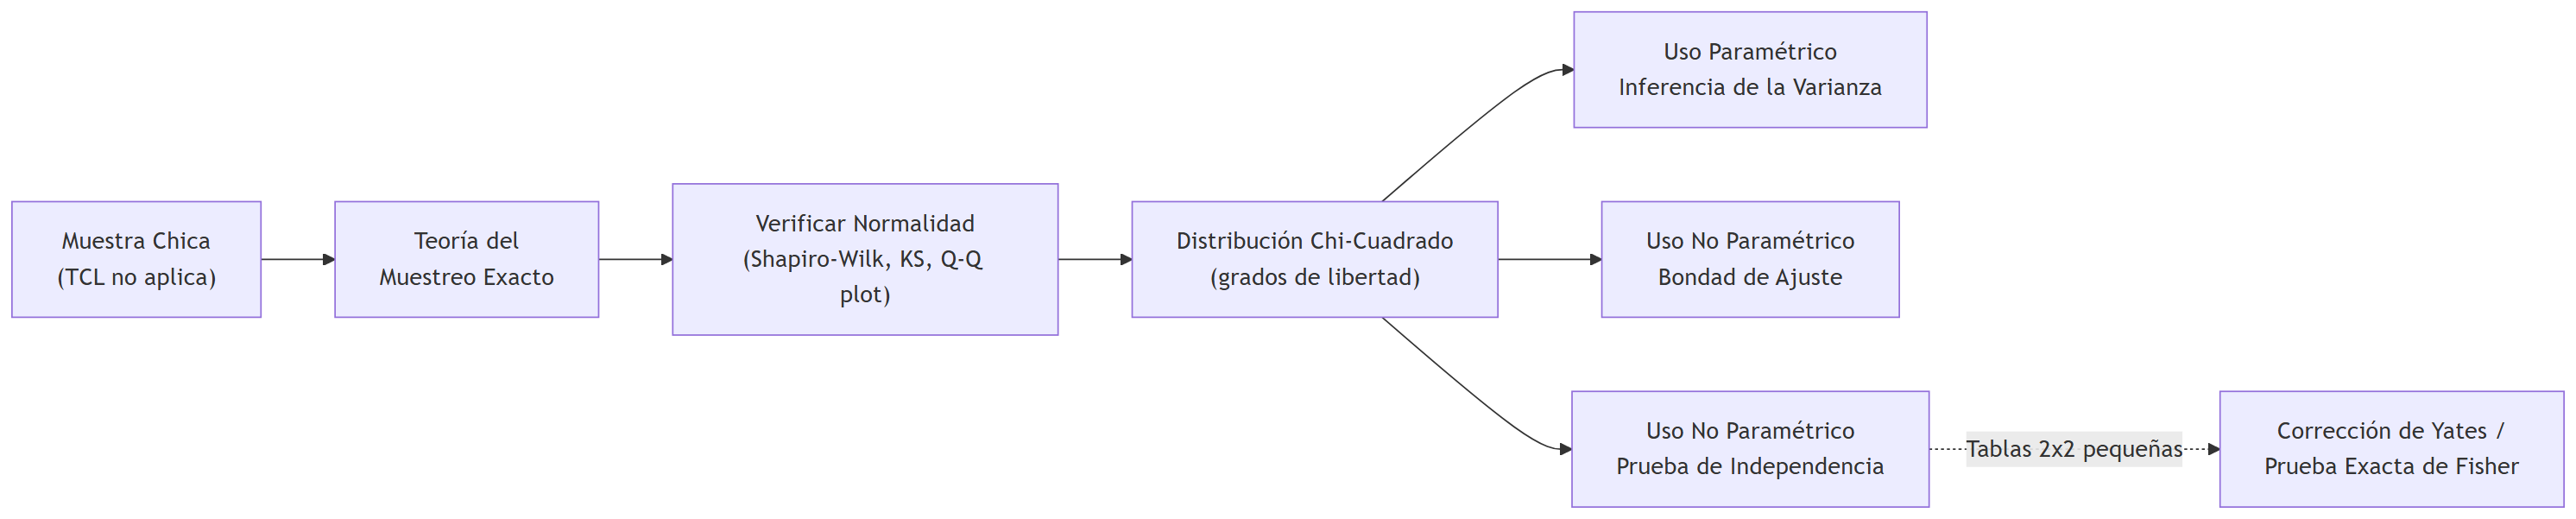
\includegraphics[width=18.1in,height=3.65in]{09_inferencia_muestras_chicas_chi_files/figure-latex/mermaid-figure-1.png}

Marco conceptual de la Unidad de Inferencia con Muestras Chicas
(Chi-Cuadrado)

\section{\texorpdfstring{\textbf{Actividad de
pre-clase}}{Actividad de pre-clase}}\label{actividad-de-pre-clase-3}

Deberá subir las siguientes producciones realizadas durante la cursada
de Epistemología 2026 al cuaderno de \emph{notebooklm}, y preguntarle
cuál es la pregunta de investigación y los objetivos propuestos en cada
uno. En clase se le pedirá que conteste a estas preguntas.

\begin{itemize}
\tightlist
\item
  \href{./TRABAJOS\%20EPIST/006_chi/Grupo\%203_Sem\%202_2026.docx}{GRUPO
  3}
\item
  \href{./TRABAJOS\%20EPIST/006_chi/Ecology\%20Journal-Vol.\%206\%20No.\%202\%20(2024)1738334681.pdf}{Ecology
  Journal-Vol. 6 No.~2 (2024)1738334681.pdf}
\item
  \href{./TRABAJOS\%20EPIST/006_chi/Grupo\%205_SEMINARIO\%202_22-06-26\%20(2).docx}{GRUPO
  5}
\item
  \href{./TRABAJOS\%20EPIST/006_chi/GRUPO\%2012_SEMINARIO2_2026.docx}{GRUPO
  12}
\item
  \href{./TRABAJOS\%20EPIST/006_chi/GRUPO\%2014_SEM2_2026.docx}{GRUPO
  14}
\item
  \href{./TRABAJOS\%20EPIST/006_chi/006_chi_2026.r}{SCRIPT DE R}
\end{itemize}

\section{Micro-ejercicios de aplicación
(optativos)}\label{micro-ejercicios-de-aplicaciuxf3n-optativos-6}

Los siguientes son ejercicios tomados de algunos de los recursos
bibliográficos sugeridos.

\begin{Shaded}
\begin{Highlighting}[]
\CommentTok{\# Inferencia de la varianza poblacional ($\textbackslash{}sigma\^{}2$ / desvío estándar):}
\CommentTok{\# }
\CommentTok{\# Ejemplo 1: Estimación por IC del 95\% para la varianza en residuos de plaguicidas en leche (Apuntes Bioestadística CER, pág. 358).}
\CommentTok{\# Ejemplo 2: Prueba de hipótesis para la desviación estándar en máquinas embotelladoras (Triola, pág. 438).}
\CommentTok{\# Ejemplo 3: Intervalo de confianza del 99\% para la variabilidad del mamífero más pequeño del mundo (Triola, pág. 374).}
\CommentTok{\# Ejemplo 4: Estimación de la desviación estándar sobre el índice de masa corporal (IMC). (Triola, pág. 374).}
\CommentTok{\# }
\CommentTok{\# Prueba de independencia (Tablas de contingencia):}
\CommentTok{\# }
\CommentTok{\# Ejemplo 1: Asociación entre raza vacuna y éxito de fecundidad (Apuntes Bioestadística CER, pág. 363).}
\CommentTok{\# Ejemplo 2: Independencia entre contenido de sacarosa y aptitud industrial en caña de azúcar (Apuntes Bioestadística CER, pág. 370).}
\CommentTok{\# Ejemplo 3: Relación entre condición corporal de vacas y éxito en inseminación artificial (Balzarini et al., pág. 274).}
\CommentTok{\# Ejemplo 4: Evaluación de la exactitud de pruebas poligráficas (Triola, pág. 618).}
\CommentTok{\# Ejemplo 5: Prueba de detección de cáncer de vejiga mediante perros entrenados (Triola, pág. 618).}
\CommentTok{\# }
\CommentTok{\# Ajuste a distribución teórica (Poisson, Binomial, Normal):}
\CommentTok{\# }
\CommentTok{\# Ejemplo 1: Prueba de bondad de ajuste a un modelo discreto Binomial (n=3, p=1/3) (Triola, pág. 605).}
\CommentTok{\# Ejemplo 2: Ajuste de frecuencias observadas de CI a una distribución Normal (mu=100, sigma=15) (Triola, págs. 605{-}606).}
\CommentTok{\# Ejemplo 3: Prueba de concordancia de datos agrupados frente a una curva Normal (Triola, pág. 605).}
\CommentTok{\# }
\CommentTok{\# Prueba de frecuencias esperadas (Proporciones teóricas / Equiprobabilidad / Vectores):}
\CommentTok{\# }
\CommentTok{\# Ejemplo 1: Ajuste de proporciones fenotípicas observadas al ratio mendeliano 1:2:1 (Apuntes Bioestadística CER, pág. 362).}
\CommentTok{\# Ejemplo 2: Segregación independiente de 3 caracteres mendelianos con 8 clases fenotípicas (Balzarini et al., pág. 255).}
\CommentTok{\# Ejemplo 3: Prueba de equiprobabilidad en las 6 caras de un dado cargado (Triola, pág. 601).}
\CommentTok{\# Ejemplo 4: Verificación de frecuencias genotípicas observadas frente al modelo 25\%{-}50\%{-}25\% (Triola, pág. 604).}
\CommentTok{\# Ejemplo 5: Contraste de frecuencias observadas de color de ojos frente a proporciones teóricas predichas (Triola, pág. 603).}
\end{Highlighting}
\end{Shaded}

\bookmarksetup{startatroot}

\chapter{Trabajo Práctico 7: Inferencia con Muestras Chicas:
Distribuciones F de Snedecor y t de
Student}\label{trabajo-pruxe1ctico-7-inferencia-con-muestras-chicas-distribuciones-f-de-snedecor-y-t-de-student}

Objetivos del Trabajo Práctico Al finalizar esta unidad, el estudiante
deberá comprender y utilizar las distribuciones F y t de Student como
técnicas de inferencia en muestras pequeñas provenientes de poblaciones
normales. En particular, se busca que el estudiante sea capaz de: (1)
Reconocer los contextos en los que corresponde utilizar cada
distribución, en función del tamaño muestral, el tipo de parámetro de
interés y la información disponible; (2) Comprender la construcción de
los estadísticos asociados a ambas distribuciones y el rol de los grados
de libertad en su comportamiento; (3) Aplicar la distribución t en la
estimación de medias (intervalos de confianza) y en contrastes de
hipótesis para una y dos muestras, interpretando correctamente los
resultados; (4) Utilizar la distribución F para comparar varianzas, como
base del análisis de varianza (ANOVA); (5) Interpretar los resultados de
los contrastes en términos del problema aplicado, evitando una lectura
meramente mecánica del p-valor; y (6) Evaluar los supuestos involucrados
(normalidad, independencia, homogeneidad de varianzas) y su impacto
sobre la validez de las conclusiones.

\begin{tcolorbox}[enhanced jigsaw, arc=.35mm, bottomrule=.15mm, bottomtitle=1mm, breakable, colback=white, colbacktitle=quarto-callout-important-color!10!white, colframe=quarto-callout-important-color-frame, coltitle=black, left=2mm, leftrule=.75mm, opacityback=0, opacitybacktitle=0.6, rightrule=.15mm, title=\textcolor{quarto-callout-important-color}{\faExclamation}\hspace{0.5em}{Lectura Sugerida para el Trabajo Práctico}, titlerule=0mm, toprule=.15mm, toptitle=1mm]

Se recomienda a los estudiantes consultar los siguientes recursos para
profundizar los conceptos metodológicos desarrollados en este marco:

\begin{itemize}
\tightlist
\item
  \textbf{Solís, J.M.} \emph{«Apuntes de Bioestadística, Con Ejercicios
  Resueltos»}: unidad 9 \emph{«Inferencia Estadística con muestras
  pequeñas. Distribuciones F y t.»}.
\item
  \textbf{Irizarry, R. A.} \emph{«Data Analysis for the Life Sciences»}:
  unidad \emph{«Inference»}.
\item
  \textbf{Weaver et al.}: unidad \emph{«t-test»}.
\item
  \textbf{Lepš, J. y Šmilauer, P.} \emph{«Biostatistics with R»}:
  unidades 5 y 6.
\item
  \textbf{Balzarini et al.} \emph{«Estadística y Biometría»}: unidad
  \emph{«Comparación de dos poblaciones»}.
\end{itemize}

\end{tcolorbox}

\section{Generalidades}\label{generalidades-5}

En la unidad anterior se presentó la Teoría del Muestreo Exacto a partir
de la distribución Chi-cuadrado. En esta unidad se completa ese marco
con dos distribuciones más: la \textbf{F de Snedecor} y la \textbf{t de
Student}. Ambas permiten realizar inferencia con validez exacta en
muestras pequeñas, siempre que la variable de interés provenga de una
población \textbf{normal}, y ambas quedan definidas por sus
\textbf{grados de libertad}.

\subsection{La distribución F de
Snedecor}\label{la-distribuciuxf3n-f-de-snedecor}

La distribución F es la distribución del cociente entre dos variables
Chi-cuadrado. Su aplicación central es la \textbf{comparación de
varianzas} entre grupos: dadas dos muestras independientes de
poblaciones normales, el cociente de sus varianzas muestrales sigue una
distribución F con dos parámetros, los grados de libertad del numerador
y del denominador. Es una distribución asimétrica positiva, y su alcance
excede la comparación de dos varianzas: es la base de los contrastes en
el \textbf{análisis de varianza (ANOVA)} y en regresión, que serán
retomados en unidades posteriores. Una advertencia importante es que la
prueba F es especialmente sensible a los desvíos de la normalidad.

\subsection{La distribución t de
Student}\label{la-distribuciuxf3n-t-de-student}

La distribución t es la alternativa para la inferencia sobre
\textbf{medias} cuando la variable es normal, el tamaño muestral es
pequeño (o no es aplicable el Teorema Central del Límite) y el desvío
estándar poblacional es \textbf{desconocido}. Es simétrica, con forma de
campana similar a la Normal pero con colas más pesadas, y se aproxima a
la Normal a medida que aumentan los grados de libertad. Con ella es
posible realizar estimación puntual, intervalos de confianza y
contrastes de hipótesis para una media, y para la diferencia entre dos
medias en tres situaciones: grupos independientes con varianzas
homogéneas, grupos independientes con varianzas heterogéneas, y grupos
apareados.

\subsection{Supuestos y orden de
trabajo}\label{supuestos-y-orden-de-trabajo}

Los procedimientos de esta unidad asumen normalidad, independencia de
las observaciones (salvo en el caso de grupos apareados, donde se
trabaja sobre las diferencias) y, en una de las versiones de la prueba t
para dos muestras, homogeneidad de varianzas. Por ello, resulta
indispensable \textbf{verificar los supuestos antes de inferir}: la
normalidad mediante la prueba de Shapiro-Wilk y el gráfico Q-Q, y la
homogeneidad de varianzas mediante la prueba F.

La comparación de varianzas puede ser un \textbf{objetivo en sí mismo}
(por ejemplo, evaluar si un tratamiento modifica la variabilidad de una
respuesta), pero también funciona como \textbf{prueba a priori} al
comparar dos medias de grupos independientes: su resultado indica qué
versión de la prueba t corresponde aplicar, con varianza combinada si
las varianzas son homogéneas, o con grados de libertad ajustados
(Satterthwaite) si no lo son.

Finalmente, en todos los casos el resultado de cada contraste debe
interpretarse en términos del problema aplicado, y no limitarse a
comparar el p-valor con el nivel de significación.

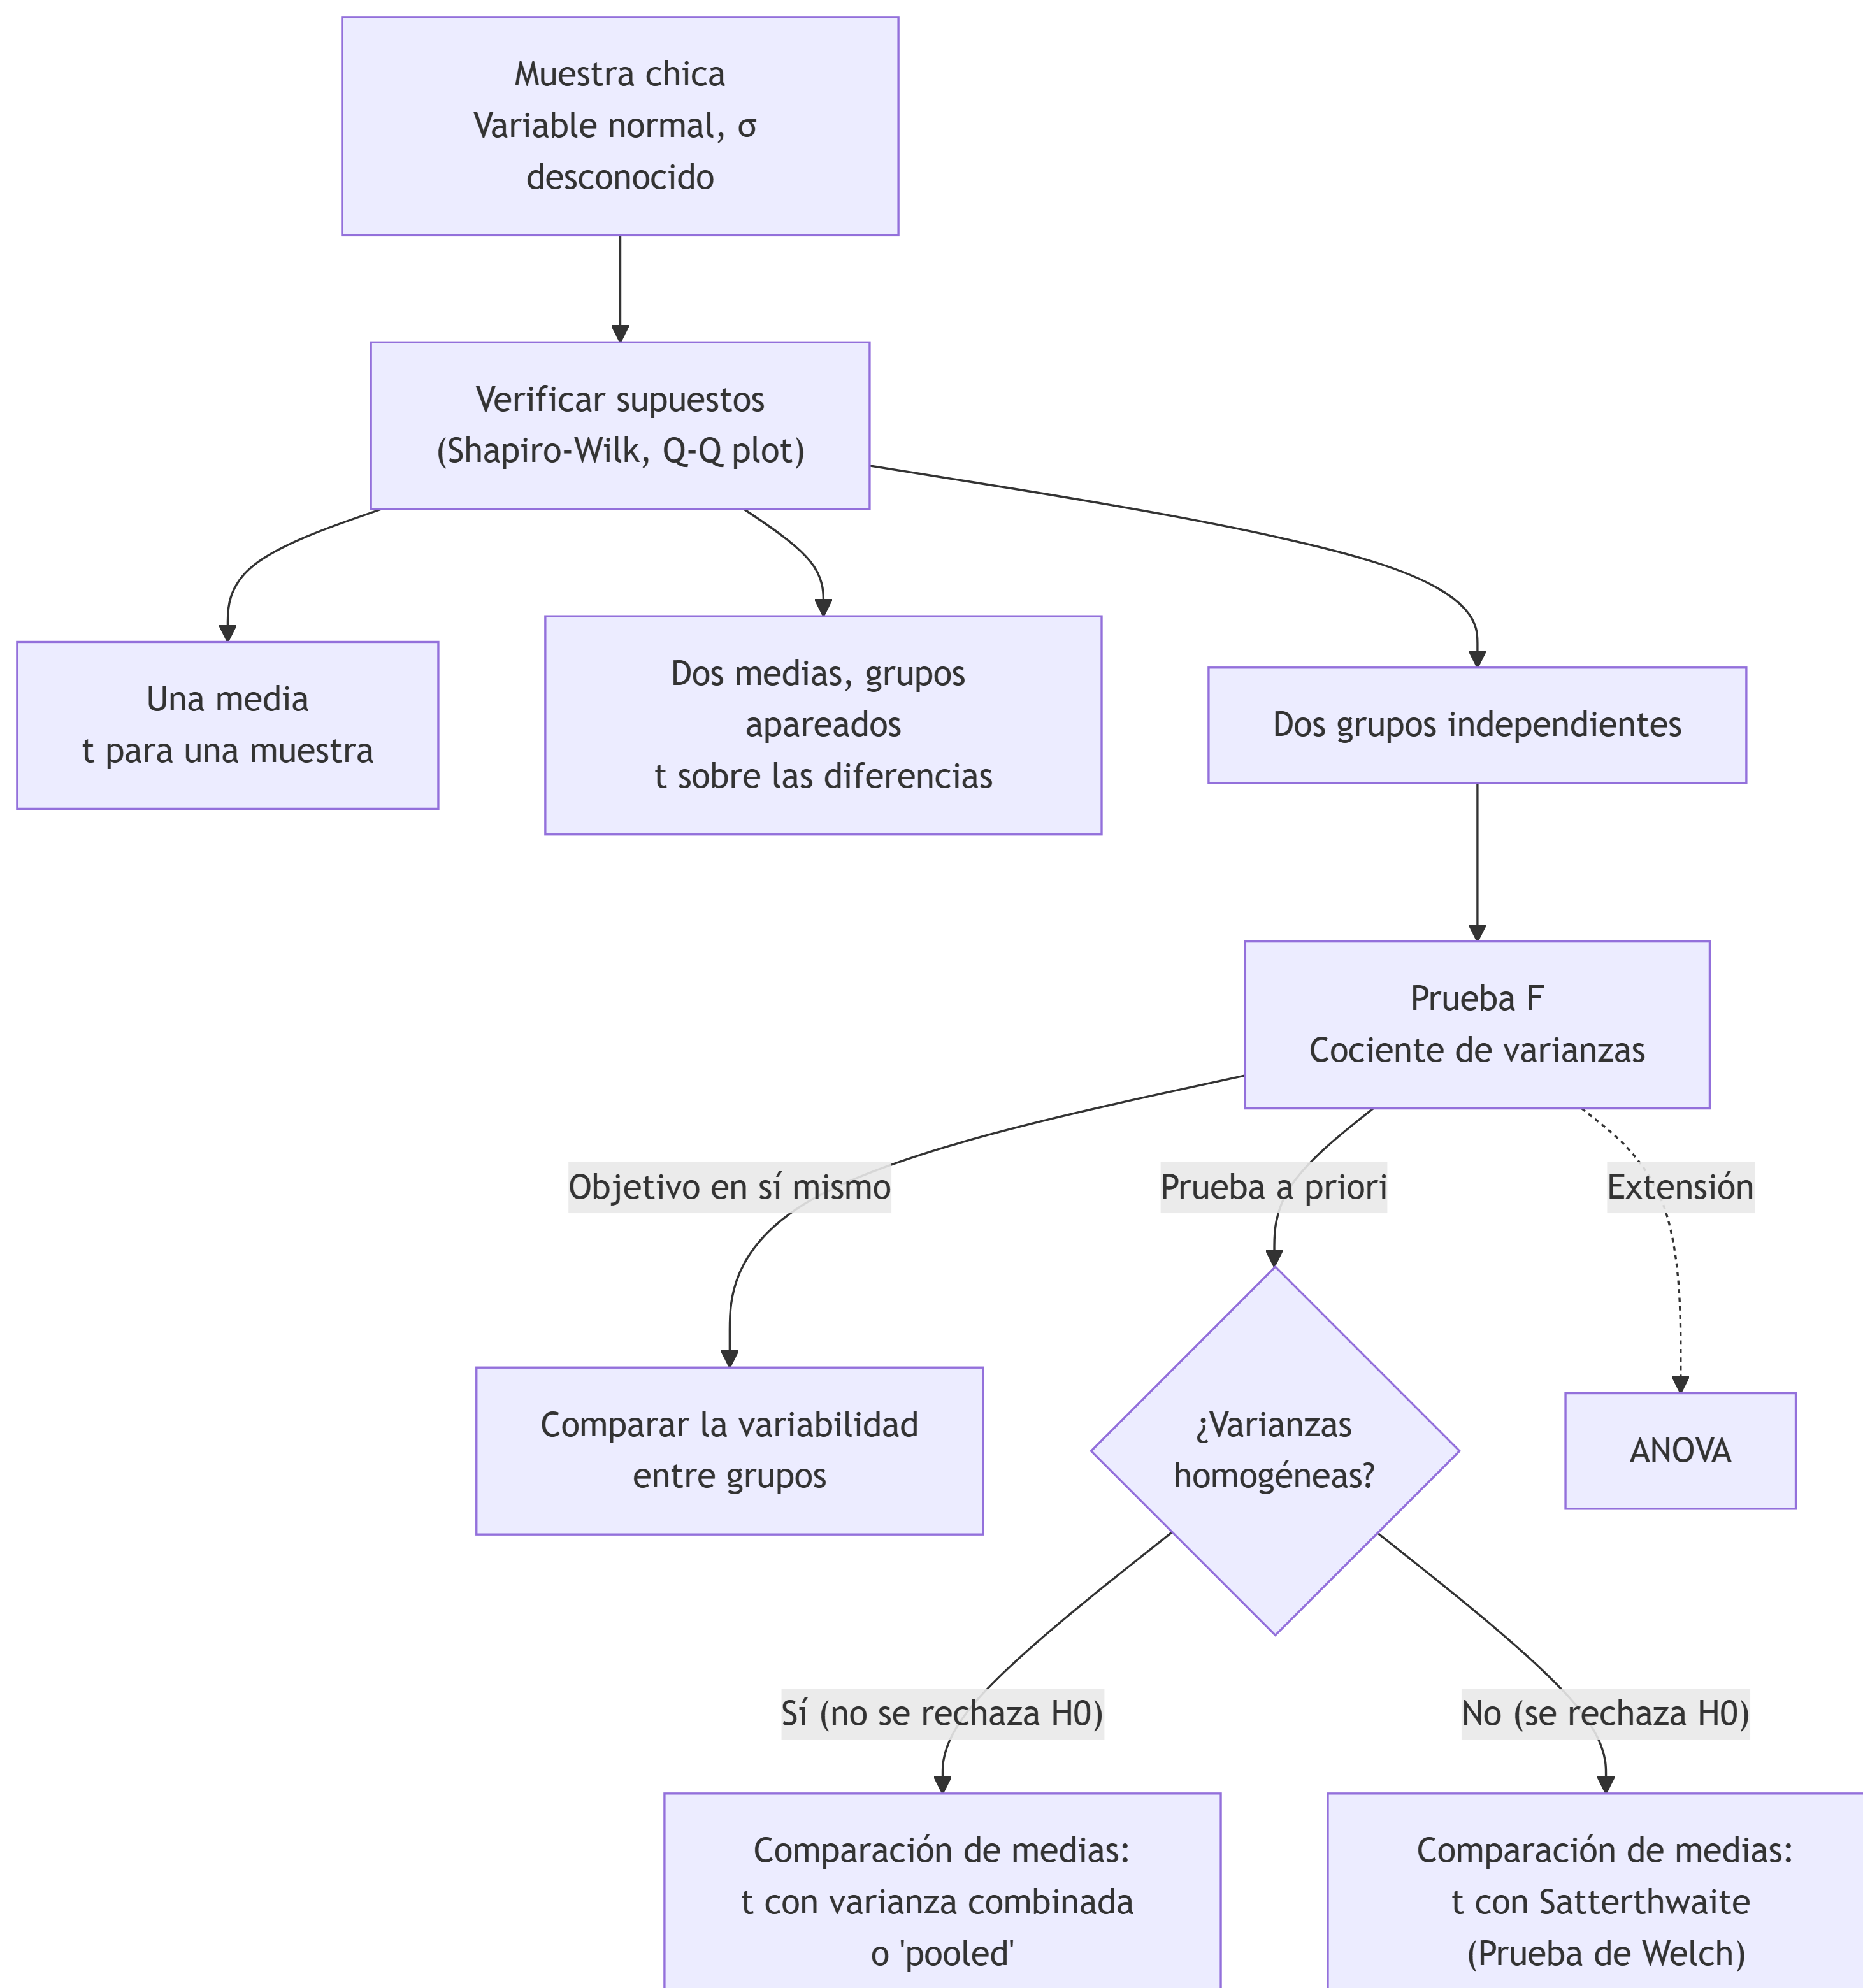
\includegraphics[width=9.26in,height=9.88in]{10_inferencia_muestras_chicas_tyf_files/figure-latex/mermaid-figure-1.png}

Marco conceptual de la Unidad de Inferencia con Muestras Chicas (F y t)

\section{\texorpdfstring{\textbf{Actividad de
pre-clase}}{Actividad de pre-clase}}\label{actividad-de-pre-clase-4}

Deberá subir las siguientes producciones realizadas durante la cursada
de Epistemología 2026 al cuaderno de \emph{notebooklm}, y preguntarle
cuál es la pregunta de investigación y los objetivos propuestos en cada
uno de los trabajos de los grupos 6 y 14. En clase se le pedirá que
conteste a estas preguntas. Además, deberá pedirle a la IA, basándose en
los ejercicios guiados de la primera parte del script de R, que
construya un flujo de trabajo común, transversal a las 5 situaciones
ejemplificadas, que le permitan esquematizar sus análisis.

\begin{itemize}
\tightlist
\item
  \href{./TRABAJOS\%20EPIST/tyf2026/007_tyf_2026.r}{007\_tyf\_2026.r}
\item
  \href{./TRABAJOS\%20EPIST/tyf2026/GRUPO\%2014_SEM2_2026.docx}{GRUPO
  14\_SEM2\_2026.docx}
\item
  \href{./TRABAJOS\%20EPIST/tyf2026/GRUPO\%206_\%20SEMINARIO\%202_2026.docx}{GRUPO
  6\_ SEMINARIO 2\_2026.docx}
\end{itemize}

\section{Micro-ejercicios de aplicación
(optativos)}\label{micro-ejercicios-de-aplicaciuxf3n-optativos-7}

Los siguientes micro-ejercicios te permitirán practicar los conceptos
revisados en esta unidad. Puedes copiar y pegar las preguntas en un
script de R local, o bien utilizar \texttt{webR}, que es la versión
\emph{online} de R, disponible en esta guía.

\texttt{Nota}: los ejercicios están inspirados en trabajos científicos
publicados, pero contienen datos simulados. Por lo tanto, los resultados
obtenidos deben interpretarse únicamente con fines didácticos y no como
evidencia científica.

La finalidad es familiarizarse con el análisis estadístico y con el uso
de R a partir de situaciones similares a las que pueden encontrarse en
investigaciones reales.

\begin{Shaded}
\begin{Highlighting}[]

\CommentTok{\# Identifique en cada caso la prueba estadística adecuada.}


\CommentTok{\# ─────────────────────────────────────────────────────────────────────────────}
\CommentTok{\# EJERCICIO 1 {-} PESO DE 100 SEMILLAS DE QUINUA (Chenopodium quinoa)}
\CommentTok{\# ─────────────────────────────────────────────────────────────────────────────}
\CommentTok{\#}
\CommentTok{\# Se evalúa la calidad fisiológica de un ecotipo de quinua (Chenopodium quinoa) cultivado en la Puna jujeña. El peso estándar promedio de referencia para 100 semillas de esta variedad es µ₀ = 3.20 g. Un investigador toma una muestra aleatoria de 12 lotes de 100 semillas.}
\CommentTok{\#}
\CommentTok{\# Peso de 100 semillas de quinua en gramos (g):}
\NormalTok{peso\_quinua }\OtherTok{=} \FunctionTok{c}\NormalTok{(}\FloatTok{3.12}\NormalTok{, }\FloatTok{3.08}\NormalTok{, }\FloatTok{3.15}\NormalTok{, }\FloatTok{3.05}\NormalTok{, }\FloatTok{3.10}\NormalTok{, }\FloatTok{3.14}\NormalTok{, }\FloatTok{3.07}\NormalTok{, }\FloatTok{3.09}\NormalTok{, }\FloatTok{3.11}\NormalTok{, }\FloatTok{3.06}\NormalTok{, }\FloatTok{3.13}\NormalTok{, }\FloatTok{3.08}\NormalTok{)}
\CommentTok{\#}
\CommentTok{\# a) Identifique la variable aleatoria bajo estudio, su tipo y el parámetro de interés.}
\CommentTok{\# b) Plantee las hipótesis nula (H0) y alternativa (H₁) para determinar si el peso medio difiere del estándar de 3.20 g a un nivel α = 0.05.}
\CommentTok{\# c) Calcule manualmente la media muestral, la desviación estándar y el estadístico de prueba t.}
\CommentTok{\# d) Determine el p{-}valor, tome una decisión estadística y construya el intervalo de confianza bilateral del 95\%.}
\CommentTok{\# e) Verifique sus resultados utilizando la función t.test() de R e interprete la conclusión en el contexto agronómico.}

\CommentTok{\# Su código aquí:}

\CommentTok{\# ─────────────────────────────────────────────────────────────────────────────}


\CommentTok{\# ─────────────────────────────────────────────────────────────────────────────}
\CommentTok{\# EJERCICIO 2 {-} Comparación de variabilidad en el peso de frutos de pimiento}
\CommentTok{\# ─────────────────────────────────────────────────────────────────────────────}
\CommentTok{\# Un horticultor desea saber si dos modalidades de fertirriego (Sistemas A y B)}
\CommentTok{\# producen diferencias en la uniformidad (variabilidad) del peso de los frutos.}
\CommentTok{\#}
\CommentTok{\# a) Formule las hipótesis correspondientes únicamente para evaluar la variabilidad (varianzas).}
\CommentTok{\# b) Defina la variable respuesta y el factor en estudio.}
\CommentTok{\# c) Aplique la prueba F de Snedecor en R con α = 0.05.}
\CommentTok{\# d) Responda si uno de los sistemas produce frutos de peso más uniforme que el otro.}
\CommentTok{\#}
\CommentTok{\# Datos de peso de fruto (g):}
\NormalTok{x1 }\OtherTok{=} \FunctionTok{c}\NormalTok{(}\DecValTok{185}\NormalTok{, }\DecValTok{190}\NormalTok{, }\DecValTok{188}\NormalTok{, }\DecValTok{182}\NormalTok{, }\DecValTok{187}\NormalTok{, }\DecValTok{189}\NormalTok{)   }\CommentTok{\# Sistema A}
\NormalTok{x2 }\OtherTok{=} \FunctionTok{c}\NormalTok{(}\DecValTok{170}\NormalTok{, }\DecValTok{205}\NormalTok{, }\DecValTok{165}\NormalTok{, }\DecValTok{210}\NormalTok{, }\DecValTok{180}\NormalTok{, }\DecValTok{195}\NormalTok{)   }\CommentTok{\# Sistema B}

\CommentTok{\# Su código aquí:}

\CommentTok{\# ─────────────────────────────────────────────────────────────────────────────}


\CommentTok{\# ─────────────────────────────────────────────────────────────────────────────}
\CommentTok{\# EJERCICIO 3 {-} Efecto de un inoculante micorrícico en la masa radicular (Apareado)}
\CommentTok{\# ─────────────────────────────────────────────────────────────────────────────}
\CommentTok{\# Para evaluar el efecto de un inoculante con micorrizas, se midió el volumen}
\CommentTok{\# radicular (cm³) en plantines de tomate en un diseño de pares formados por}
\CommentTok{\# similitud de tamaño inicial. Un individuo de cada par recibió inoculante y el otro actuó como control.}
\CommentTok{\#}
\CommentTok{\# a) ¿Por qué este diseño requiere una prueba t de Student para muestras apareadas?}
\CommentTok{\# b) Plantee H0 y H₁ para evaluar si el inoculante incrementa el volumen radicular.}
\CommentTok{\# c) Ejecute la prueba t apareada en R usando alfa = 0.01.}
\CommentTok{\# d) Redacte la conclusión biológica en función del p{-}valor hallado.}
\CommentTok{\#}
\CommentTok{\# Datos de volumen radicular (cm³):}
\NormalTok{x1 }\OtherTok{=} \FunctionTok{c}\NormalTok{(}\FloatTok{12.3}\NormalTok{, }\FloatTok{14.1}\NormalTok{, }\FloatTok{11.5}\NormalTok{, }\FloatTok{13.0}\NormalTok{, }\FloatTok{15.2}\NormalTok{, }\FloatTok{12.8}\NormalTok{)   }\CommentTok{\# Control}
\NormalTok{x2 }\OtherTok{=} \FunctionTok{c}\NormalTok{(}\FloatTok{15.0}\NormalTok{, }\FloatTok{16.8}\NormalTok{, }\FloatTok{13.9}\NormalTok{, }\FloatTok{15.5}\NormalTok{, }\FloatTok{18.0}\NormalTok{, }\FloatTok{15.1}\NormalTok{)   }\CommentTok{\# Inoculado}

\CommentTok{\# Su código aquí:}

\CommentTok{\# ─────────────────────────────────────────────────────────────────────────────}


\CommentTok{\# ─────────────────────────────────────────────────────────────────────────────}
\CommentTok{\# EJERCICIO 4 {-} Comparación de la capacidad de germinación en dos lotes de semilla}
\CommentTok{\# ─────────────────────────────────────────────────────────────────────────────}
\CommentTok{\# Un laboratorio de análisis de semillas evalúa el vigor germinativo (\%) de dos}
\CommentTok{\# lotes de semillas de maíz (Lote 1 y Lote 2) almacenados bajo distintas condiciones.}
\CommentTok{\#}
\CommentTok{\# a) Identifique las variables, los objetivos y plantee las hipótesis H0 y H₁.}
\CommentTok{\# b) Verifique la homogeneidad de varianzas entre ambos lotes con la prueba F (α = 0.05).}
\CommentTok{\# c) Realice la prueba t de Student adecuada según el resultado de las varianzas.}
\CommentTok{\# d) Interprete el p{-}valor obtenido y elabore una conclusión técnico{-}agronómica.}
\CommentTok{\#}
\CommentTok{\# Datos de porcentaje de germinación (\%):}
\NormalTok{x1 }\OtherTok{=} \FunctionTok{c}\NormalTok{(}\DecValTok{88}\NormalTok{, }\DecValTok{92}\NormalTok{, }\DecValTok{85}\NormalTok{, }\DecValTok{89}\NormalTok{, }\DecValTok{90}\NormalTok{, }\DecValTok{87}\NormalTok{)   }\CommentTok{\# Lote 1}
\NormalTok{x2 }\OtherTok{=} \FunctionTok{c}\NormalTok{(}\DecValTok{78}\NormalTok{, }\DecValTok{82}\NormalTok{, }\DecValTok{80}\NormalTok{, }\DecValTok{75}\NormalTok{, }\DecValTok{84}\NormalTok{, }\DecValTok{79}\NormalTok{)   }\CommentTok{\# Lote 2}

\CommentTok{\# Su código aquí:}

\CommentTok{\# ─────────────────────────────────────────────────────────────────────────────}


\CommentTok{\# ─────────────────────────────────────────────────────────────────────────────}
\CommentTok{\# EJERCICIO 5 {-} DIÁMETRO A LA ALTURA DEL PECHO EN ALGARROBO BLANCO (Prosopis alba)}
\CommentTok{\# ─────────────────────────────────────────────────────────────────────────────}
\CommentTok{\#}
\CommentTok{\# En un proyecto de restauración ecológica en la cuenca del Río Grande, se mide el Diámetro a la Altura del Pecho (DAP) en una parcela de regeneración de algarrobo blanco (Prosopis alba). Se desea verificar si el DAP medio difiere del valor objetivo de desarrollo de 12.0 cm fijado para esa etapa fenológica.}
\CommentTok{\#}
\CommentTok{\# Diámetro a la Altura del Pecho (DAP) en centímetros (cm):}
\NormalTok{dap\_algarrobo }\OtherTok{=} \FunctionTok{c}\NormalTok{(}\FloatTok{11.2}\NormalTok{, }\FloatTok{11.8}\NormalTok{, }\FloatTok{12.1}\NormalTok{, }\FloatTok{11.5}\NormalTok{, }\FloatTok{11.9}\NormalTok{, }\FloatTok{11.4}\NormalTok{, }\FloatTok{11.7}\NormalTok{, }\FloatTok{12.0}\NormalTok{, }\FloatTok{11.3}\NormalTok{, }\FloatTok{11.6}\NormalTok{, }\FloatTok{11.8}\NormalTok{, }\FloatTok{11.5}\NormalTok{, }\FloatTok{12.2}\NormalTok{, }\FloatTok{11.6}\NormalTok{)}
\CommentTok{\#}
\CommentTok{\# a) Defina la variable de interés, la unidad de medida y la hipótesis estadística a contrastar.}
\CommentTok{\# b) Plantee la prueba t para una muestra con α = 0.05.}
\CommentTok{\# c) Obtenga el estadístico t calculado, los grados de libertad y el p{-}valor correspondiente.}
\CommentTok{\# d) Construya e interprete el intervalo de confianza del 95\% para el DAP promedio poblacional.}
\CommentTok{\# e) Redacte una síntesis técnica dirigida al equipo de manejo forestal.}

\CommentTok{\# Su código aquí:}

\CommentTok{\# ─────────────────────────────────────────────────────────────────────────────}


\CommentTok{\# ─────────────────────────────────────────────────────────────────────────────}
\CommentTok{\# EJERCICIO 6 {-} Resistencia a la penetración del suelo con dos tipos de labranza}
\CommentTok{\# ─────────────────────────────────────────────────────────────────────────────}
\CommentTok{\# Se desea comprobar si la labranza reducida genera una mayor resistencia a la}
\CommentTok{\# penetración del suelo (MPa) a 20 cm de profundidad en comparación con la labranza}
\CommentTok{\# convencional. Se tomaron muestras pequeñas independientes en parcelas contiguas.}
\CommentTok{\#}
\CommentTok{\# a) Defina el tipo de prueba (unilateral o bilateral) e identifique el parámetro a comparar.}
\CommentTok{\# b) Formule H0 y H₁ considerando α = 0.05.}
\CommentTok{\# c) Evalúe la hipótesis de igualdad de varianzas.}
\CommentTok{\# d) Ejecute la prueba t para dos muestras independientes e indique la decisión final.}
\CommentTok{\#}
\CommentTok{\# Datos de resistencia a la penetración (MPa):}
\NormalTok{x1 }\OtherTok{=} \FunctionTok{c}\NormalTok{(}\FloatTok{2.4}\NormalTok{, }\FloatTok{2.7}\NormalTok{, }\FloatTok{2.9}\NormalTok{, }\FloatTok{2.5}\NormalTok{, }\FloatTok{2.8}\NormalTok{)   }\CommentTok{\# Labranza Reducida}
\NormalTok{x2 }\OtherTok{=} \FunctionTok{c}\NormalTok{(}\FloatTok{1.8}\NormalTok{, }\FloatTok{2.1}\NormalTok{, }\FloatTok{1.9}\NormalTok{, }\FloatTok{2.0}\NormalTok{, }\FloatTok{1.7}\NormalTok{)   }\CommentTok{\# Labranza Convencional}

\CommentTok{\# Su código aquí:}

\CommentTok{\# ─────────────────────────────────────────────────────────────────────────────}


\CommentTok{\# ─────────────────────────────────────────────────────────────────────────────}
\CommentTok{\# EJERCICIO 7 {-} CONCENTRACIÓN DE CLOROFILA TOTAL EN Nicotiana tabacum}
\CommentTok{\# ─────────────────────────────────────────────────────────────────────────────}
\CommentTok{\#}
\CommentTok{\# Se evalúa el efecto del estrés hídrico moderado en plantas de tabaco (Nicotiana tabacum). En condiciones normales de riego, la concentración media histórica de clorofila total es de µ₀ = 45.0 µg/cm². Se mide la concentración foliar de clorofila en 10 plantas sometidas al tratamiento hídrico restringido.}
\CommentTok{\#}
\CommentTok{\# Concentración de clorofila total medida en microgramos por centímetro cuadrado (µg/cm²):}
\NormalTok{clorofila }\OtherTok{=} \FunctionTok{c}\NormalTok{(}\FloatTok{41.2}\NormalTok{, }\FloatTok{43.5}\NormalTok{, }\FloatTok{39.8}\NormalTok{, }\FloatTok{42.0}\NormalTok{, }\FloatTok{40.5}\NormalTok{, }\FloatTok{41.8}\NormalTok{, }\FloatTok{42.2}\NormalTok{, }\FloatTok{38.9}\NormalTok{, }\FloatTok{40.1}\NormalTok{, }\FloatTok{41.0}\NormalTok{)}
\CommentTok{\#}
\CommentTok{\# a) Indique la variable explicativa y la variable respuesta, detallando la escala de medición.}
\CommentTok{\# b) Formule las hipótesis H0 y H₁ con notación matemática adecuada (µ₀ = 45.0 µg/cm²).}
\CommentTok{\# c) Implemente en R el cálculo manual del estadístico tc, p{-}valor e intervalo de confianza del 95\%.}
\CommentTok{\# d) Aplique la función t.test() para contrastar los resultados obtenidos manualmente.}
\CommentTok{\# e) ¿Qué efecto biológico sobre el aparato fotosintético sugiere la evidencia observada?}

\CommentTok{\# Su código aquí:}

\CommentTok{\# ─────────────────────────────────────────────────────────────────────────────}


\CommentTok{\# ─────────────────────────────────────────────────────────────────────────────}
\CommentTok{\# EJERCICIO 8 {-} TIEMPO DE METAMORFOSIS EN RENACUAJOS DE Gastrotheca christiani}
\CommentTok{\# ─────────────────────────────────────────────────────────────────────────────}
\CommentTok{\#}
\CommentTok{\# En un estudio ecofisiológico en bosques de Yungas, se registra la duración en días de la fase larval de la rana marsupial (Gastrotheca christiani). El tiempo medio de metamorfosis reportado como patrón de referencia es µ₀ = 60 días. Se analizan 15 individuos criado en condiciones de microhábitat controlado.}
\CommentTok{\#}
\CommentTok{\# Tiempo de metamorfosis registrado en días (días):}
\NormalTok{dias\_metamorfosis }\OtherTok{=} \FunctionTok{c}\NormalTok{(}\DecValTok{56}\NormalTok{, }\DecValTok{58}\NormalTok{, }\DecValTok{55}\NormalTok{, }\DecValTok{57}\NormalTok{, }\DecValTok{59}\NormalTok{, }\DecValTok{54}\NormalTok{, }\DecValTok{58}\NormalTok{, }\DecValTok{56}\NormalTok{, }\DecValTok{57}\NormalTok{, }\DecValTok{55}\NormalTok{, }\DecValTok{60}\NormalTok{, }\DecValTok{56}\NormalTok{, }\DecValTok{57}\NormalTok{, }\DecValTok{58}\NormalTok{, }\DecValTok{55}\NormalTok{)}
\CommentTok{\#}
\CommentTok{\# a) Identifique la unidad experimental, la variable medida y el tamaño de muestra (n).}
\CommentTok{\# b) Establezca las hipótesis estadísticas bilaterales a un nivel de significación del 5\% (α = 0.05).}
\CommentTok{\# c) Calcule el estadístico de prueba t y determine si cae en la región de rechazo.}
\CommentTok{\# d) Construya el intervalo de confianza bilateral al 95\% para la media del tiempo de metamorfosis.}
\CommentTok{\# e) Elabore la conclusión biológica vinculando el resultado con las condiciones del microhábitat.}

\CommentTok{\# Su código aquí:}

\CommentTok{\# ─────────────────────────────────────────────────────────────────────────────}


\CommentTok{\# ─────────────────────────────────────────────────────────────────────────────}
\CommentTok{\# EJERCICIO 9 {-} CONCENTRACIÓN DE FLAVONOIDES TOTALES EN Polylepis tomentella}
\CommentTok{\# ─────────────────────────────────────────────────────────────────────────────}
\CommentTok{\#}
\CommentTok{\# Se analiza el contenido de metabolitos secundarios (flavonoides totales) en extractos foliares de queñoa (Polylepis tomentella) provenientes de la Prepuna. El estándar de calidad para extractos medicinales requiere un nivel medio de µ₀ = 18.50 mg/g de tejido seco. Se analiza una muestra de 11 arbustos.}
\CommentTok{\#}
\CommentTok{\# Concentración de flavonoides en miligramos por gramo de tejido seco (mg/g):}
\NormalTok{flavonoides }\OtherTok{=} \FunctionTok{c}\NormalTok{(}\FloatTok{16.8}\NormalTok{, }\FloatTok{17.2}\NormalTok{, }\FloatTok{16.5}\NormalTok{, }\FloatTok{17.0}\NormalTok{, }\FloatTok{16.9}\NormalTok{, }\FloatTok{17.4}\NormalTok{, }\FloatTok{16.6}\NormalTok{, }\FloatTok{17.1}\NormalTok{, }\FloatTok{16.7}\NormalTok{, }\FloatTok{17.3}\NormalTok{, }\FloatTok{16.8}\NormalTok{)}
\CommentTok{\#}
\CommentTok{\# a) Plantee las hipótesis nula y alternativa para el contenido medio de flavonoides a α = 0.05.}
\CommentTok{\# b) Compute la media muestral, el desvío estándar muestral y el error estándar de la media.}
\CommentTok{\# c) Calcule el valor del estadístico t, los grados de libertad y el p{-}valor bilateral.}
\CommentTok{\# d) Indique si la concentración media observada satisface el estándar de calidad requerido (µ₀ = 18.50 mg/g).}
\CommentTok{\# e) Ejecute la verificación mediante t.test() en R y redacte la síntesis final del problema.}

\CommentTok{\# Su código aquí:}

\CommentTok{\# =============================================================================}
\end{Highlighting}
\end{Shaded}

\bookmarksetup{startatroot}

\chapter{Trabajo Práctico 8: Análisis de Correlación y
Regresión}\label{trabajo-pruxe1ctico-8-anuxe1lisis-de-correlaciuxf3n-y-regresiuxf3n}

Objetivos del Trabajo Práctico Esta unidad tiene como objetivos que el
estudiante sea capaz de: (1) Cuantificar e interpretar la intensidad y
dirección de la asociación lineal entre dos variables numéricas mediante
el coeficiente de correlación de Pearson, distinguiendo entre asociación
y causalidad; (2) Formular, estimar e interpretar un modelo de regresión
lineal simple, identificando el significado de sus parámetros (pendiente
e intercepto) en el contexto del problema; (3) Evaluar la calidad del
ajuste del modelo mediante medidas como el coeficiente de determinación
\(R^2\), analizando su alcance y limitaciones; (4) Analizar los
supuestos del modelo de regresión lineal (linealidad, independencia,
homocedasticidad y normalidad de los errores) a partir de herramientas
gráficas y analíticas; y (5) Utilizar el modelo ajustado para realizar
predicciones e inferencias, interpretando los resultados en términos del
fenómeno estudiado y reconociendo el alcance de la extrapolación.

\begin{tcolorbox}[enhanced jigsaw, arc=.35mm, bottomrule=.15mm, bottomtitle=1mm, breakable, colback=white, colbacktitle=quarto-callout-important-color!10!white, colframe=quarto-callout-important-color-frame, coltitle=black, left=2mm, leftrule=.75mm, opacityback=0, opacitybacktitle=0.6, rightrule=.15mm, title=\textcolor{quarto-callout-important-color}{\faExclamation}\hspace{0.5em}{Lectura Sugerida para el Trabajo Práctico}, titlerule=0mm, toprule=.15mm, toptitle=1mm]

Se recomienda a los estudiantes consultar los siguientes recursos para
profundizar los conceptos metodológicos desarrollados en este marco:

\begin{itemize}
\tightlist
\item
  \textbf{Solís, J.M.} \emph{«Apuntes de Bioestadística, Con Ejercicios
  Resueltos»}: unidad 10 \emph{«Análisis de correlación y regresión.»}.
\item
  \textbf{Lepš, J. y Šmilauer, P.} \emph{«Biostatistics with R»}:
  unidades 12 y 13.
\item
  \textbf{Weaver et al.}: unidades 10 y 11.
\item
  \textbf{Balzarini et al.} \emph{«Estadística y Biometría»}: unidad
  \emph{«Análisis de regresión»}.
\end{itemize}

\end{tcolorbox}

\section{Generalidades}\label{generalidades-6}

En esta unidad se extiende el análisis a poblaciones
\textbf{bivariantes}, es decir, aquellas en las que cada unidad
elemental aporta dos mediciones numéricas. En la unidad de Chi-cuadrado
ya se había realizado un tratamiento bivariado, pero con variables
categóricas (pruebas de independencia y de homogeneidad). Ahora ambas
variables son cuantitativas, y la asociación entre ellas puede abordarse
desde dos enfoques complementarios: el \textbf{análisis de correlación
lineal} y el \textbf{análisis de regresión}. En este Trabajo Práctico se
trabaja con el caso más simple, la regresión lineal con una única
variable predictora.

\subsection{Correlación lineal:
concepto}\label{correlaciuxf3n-lineal-concepto}

La correlación lineal es una medida del grado y el sentido de la
asociación lineal entre dos variables numéricas: indica si, cuando una
variable cambia, la otra tiende a cambiar también de forma lineal y en
una dirección determinada. En este enfoque no se distingue entre
variable dependiente e independiente. Se cuantifica mediante el
\textbf{coeficiente de correlación de Pearson (r)}, estimador del
coeficiente poblacional (ρ), y es posible contrastar mediante una prueba
de hipótesis si la correlación poblacional es distinta de cero, positiva
o negativa. El primer paso de cualquier análisis bivariado es el
\textbf{diagrama de dispersión}, cuyo patrón de puntos informa sobre la
fuerza y la dirección de la relación antes de calcular cualquier medida.
Cabe recordar que una correlación mide asociación, no causalidad.

\subsection{Estimación del modelo de Regresión lineal
simple}\label{estimaciuxf3n-del-modelo-de-regresiuxf3n-lineal-simple}

La regresión lineal simple busca la recta que mejor ajusta a los datos,
para estimar la media de una variable respuesta (Y) a partir de una
variable predictora (X) cuando la relación entre ambas es lineal. Se
trata de una relación con una compornente determinística y una
componente no determinística: a la parte explicada por la recta se le
suma un término aleatorio (el residuo), sobre el que se asume
normalidad, independencia y varianza constante. Los parámetros del
modelo tienen una lectura directa en el problema: la \textbf{pendiente}
indica cuántas unidades cambia Y por cada incremento unitario de X, y el
\textbf{intercepto} es el valor esperado de Y cuando X vale cero. La
calidad del ajuste se resume con el \textbf{coeficiente de determinación
(\(R^2\))}, que expresa la proporción de la variabilidad de Y explicada
por X; un \(R^2\) bajo indica que, aun siendo válido el modelo, su
utilidad práctica puede ser limitada. Por ejemplo, la relación entre el
ancho y el largo de las hojas de un árbol, o entre la biomasa y el
rendimiento de un cultivo, pueden abordarse con este esquema.

\subsection{Diagnóstico, predicción y sus
límites}\label{diagnuxf3stico-predicciuxf3n-y-sus-luxedmites}

Antes de interpretar un modelo es necesario evaluar si es adecuado. Para
ello se examinan gráficamente los \textbf{residuos estudentizados frente
a los valores predichos}: bajo los supuestos del modelo, deben
distribuirse al azar en torno a cero, sin patrones reconocibles. De
forma complementaria, la \textbf{distancia de Cook} permite identificar
observaciones influyentes, es decir, aquellas cuya presencia o ausencia
modifica los coeficientes ajustados en forma notoria; este punto se
menciona aquí como anticipo y se retoma en la guía de la unidad.

Una vez ajustado el modelo, puede utilizarse para predecir. Según el
interés de la investigación, la estimación se expresa de dos maneras:
mediante un \textbf{intervalo de confianza} para la respuesta media de
todas las unidades con un mismo valor de X, o mediante un
\textbf{intervalo de predicción} para una nueva observación individual,
que siempre es más amplio porque incorpora la variabilidad aleatoria
propia de cada individuo. Ambos se estrechan alrededor de los valores
medios de X e Y, y se ensanchan hacia los extremos. Por último, las
predicciones solo son confiables dentro del rango de valores de X
observado: fuera de él, la \textbf{extrapolación} carece de respaldo en
los datos. En la guía, estos análisis se resuelven con las funciones
\texttt{cor.test()}, \texttt{lm()} y \texttt{predict()} de R, y se
muestran también procedimientos equivalentes en InfoStat, LibreOffice
Calc, Python y Julia.

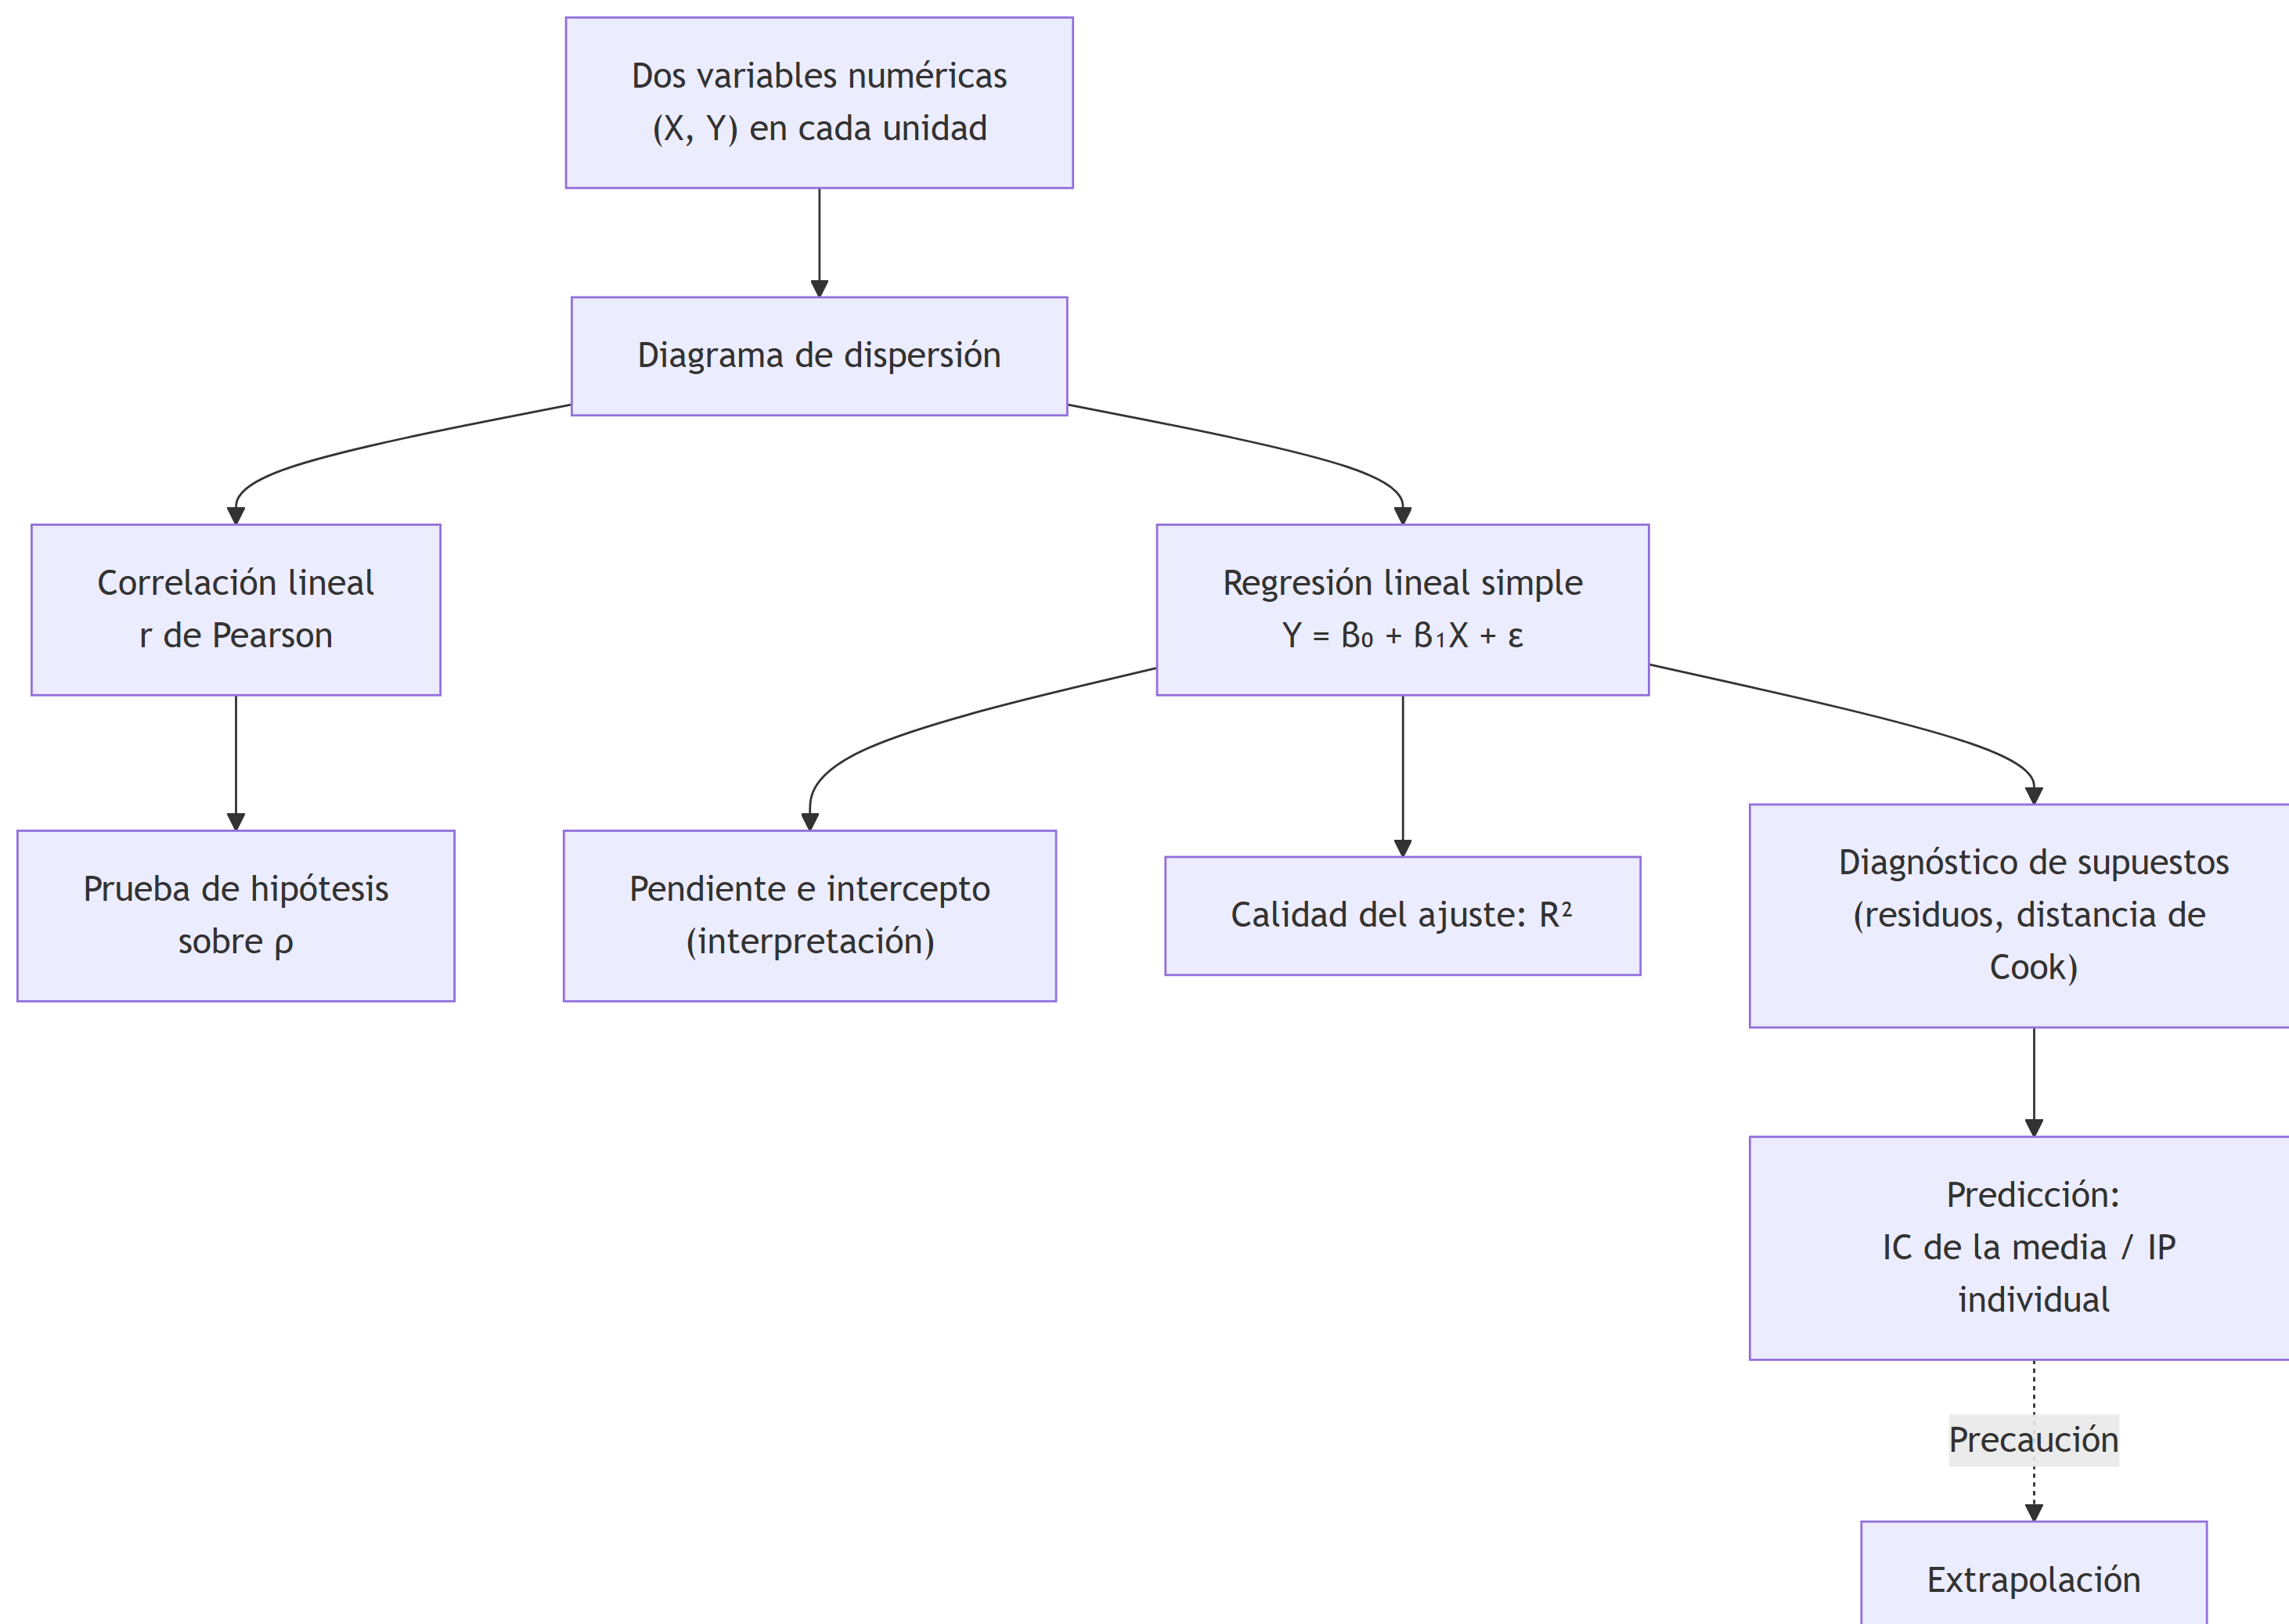
\includegraphics[width=11.13in,height=7.9in]{11_corryreg_files/figure-latex/mermaid-figure-1.png}

Marco conceptual de la Unidad de Análisis de Correlación y Regresión

\section{\texorpdfstring{\textbf{Actividad de
pre-clase}}{Actividad de pre-clase}}\label{actividad-de-pre-clase-5}

Deberá subir los siguientes archivos al cuaderno de \emph{notebooklm}, y
preguntarle cuál es la pregunta de investigación y los objetivos
propuestos en el trabajo del grupo 14.

Además, deberá pedirle a la IA, basándose en los ejercicios guiados de
la primera parte del script de R, que construya un flujo de trabajo
común que le permitan esquematizar sus análisis (la dinámica de la clase
será similar a la clase anterior).

\begin{itemize}
\tightlist
\item
  \href{./TRABAJOS\%20EPIST/reg/008_corr_y_reg_2026.r}{008\_corr\_y\_reg\_2026.r}
\item
  \href{./TRABAJOS\%20EPIST/reg/GRUPO\%2014_SEM2_2026.docx}{GRUPO
  14\_SEM2\_2026.docx}
\end{itemize}

\section{Micro-ejercicios de aplicación
(optativos)}\label{micro-ejercicios-de-aplicaciuxf3n-optativos-8}

Los siguientes micro-ejercicios te permitirán practicar los conceptos
revisados en esta unidad. Puedes copiar y pegar las preguntas en un
script de R local, o bien utilizar \texttt{webR}, que es la versión
\emph{online} de R, disponible en esta guía.

\texttt{Nota}: los ejercicios están inspirados en trabajos científicos
publicados, pero contienen datos simulados. Por lo tanto, los resultados
obtenidos deben interpretarse únicamente con fines didácticos y no como
evidencia científica.

La finalidad es familiarizarse con el análisis estadístico y con el uso
de R a partir de situaciones similares a las que pueden encontrarse en
investigaciones reales.

\begin{Shaded}
\begin{Highlighting}[]

\CommentTok{\# ─────────────────────────────────────────────────────────────────────────────}
\CommentTok{\# EJERCICIO 1 {-} LIBERACIÓN DE NITRÓGENO Y FÓSFORO SEGÚN LA PROFUNDIDAD EN EMBALSES}
\CommentTok{\# ─────────────────────────────────────────────────────────────────────────────}
\CommentTok{\#}
\CommentTok{\# Contexto: En un estudio sobre dinámica de nutrientes en embalses de agua dulce, se evalúa la relación entre la profundidad del punto de muestreo (m) y la concentración de fósforo total (mg/L) presente en la columna de agua.}
\CommentTok{\# Referencia: GRUPO 4 {-} Liberación de Nitrógeno y Fósforo por el sedimento de los embalses.}
\CommentTok{\# (Datos simulados con fines didácticos)}
\CommentTok{\#}
\CommentTok{\# Profundidad de muestreo (m):}
\NormalTok{profundidad }\OtherTok{=} \FunctionTok{c}\NormalTok{(}\DecValTok{1}\NormalTok{, }\DecValTok{3}\NormalTok{, }\DecValTok{5}\NormalTok{, }\DecValTok{8}\NormalTok{, }\DecValTok{10}\NormalTok{, }\DecValTok{12}\NormalTok{, }\DecValTok{15}\NormalTok{, }\DecValTok{18}\NormalTok{, }\DecValTok{20}\NormalTok{, }\DecValTok{22}\NormalTok{, }\DecValTok{25}\NormalTok{)}

\CommentTok{\# Concentración de Fósforo (mg/L):}
\NormalTok{fosfatos }\OtherTok{=} \FunctionTok{c}\NormalTok{(}\FloatTok{0.012}\NormalTok{, }\FloatTok{0.018}\NormalTok{, }\FloatTok{0.022}\NormalTok{, }\FloatTok{0.035}\NormalTok{, }\FloatTok{0.041}\NormalTok{, }\FloatTok{0.050}\NormalTok{, }\FloatTok{0.068}\NormalTok{, }\FloatTok{0.082}\NormalTok{, }\FloatTok{0.095}\NormalTok{, }\FloatTok{0.108}\NormalTok{, }\FloatTok{0.125}\NormalTok{)}

\CommentTok{\# a) Identifique la pregunta de investigación, los objetivos, la variable respuesta y la variable predictora.}
\CommentTok{\# b) Genere un gráfico de dispersión e interprete la relación observada entre la profundidad y la concentración de fósforo.}
\CommentTok{\# c) Calcule el coeficiente de correlación lineal de Pearson (r) e interprete su signo y magnitud.}
\CommentTok{\# d) Plantee las hipótesis H0 y H1 para evaluar si la correlación es positiva significativa (α = 0.05). Ejecute cor.test().}
\CommentTok{\# e) Justifique si corresponde ajustar un modelo de regresión lineal simple. De ser así, obtenga la recta de ajuste y R2.}
\CommentTok{\# f) Rehaga el gráfico de dispersión agregando la recta ajustada. Prediga la concentración de fósforo a 14 m de profundidad.}

\CommentTok{\# Su código aquí:}

\CommentTok{\# ─────────────────────────────────────────────────────────────────────────────}


\CommentTok{\# ─────────────────────────────────────────────────────────────────────────────}
\CommentTok{\# EJERCICIO 2 {-} RELACIÓN ENTRE TURBIDEZ Y pH EN AMBIENTES PERIGLACIARES}
\CommentTok{\# ─────────────────────────────────────────────────────────────────────────────}
\CommentTok{\#}
\CommentTok{\# Contexto: En un monitoreo de calidad de agua en arroyos de alta montaña, se investiga si existe relación entre la profundidad de visibilidad del Disco de Secchi (cm, indicador inverso de turbidez) y el pH del agua en cuencas con influencia minera.}
\CommentTok{\# Referencia: GRUPO 6 {-} Calidad de agua en ambientes periglaciares: comparación entre áreas con y sin actividad minera.}
\CommentTok{\# (Datos simulados con fines didácticos)}
\CommentTok{\#}
\CommentTok{\# Profundidad de Disco de Secchi (cm):}
\NormalTok{secchi }\OtherTok{=} \FunctionTok{c}\NormalTok{(}\DecValTok{45}\NormalTok{, }\DecValTok{50}\NormalTok{, }\DecValTok{60}\NormalTok{, }\DecValTok{65}\NormalTok{, }\DecValTok{75}\NormalTok{, }\DecValTok{80}\NormalTok{, }\DecValTok{90}\NormalTok{, }\DecValTok{95}\NormalTok{, }\DecValTok{105}\NormalTok{, }\DecValTok{110}\NormalTok{, }\DecValTok{120}\NormalTok{)}

\CommentTok{\# pH del agua:}
\NormalTok{ph }\OtherTok{=} \FunctionTok{c}\NormalTok{(}\FloatTok{5.2}\NormalTok{, }\FloatTok{5.4}\NormalTok{, }\FloatTok{5.8}\NormalTok{, }\FloatTok{6.0}\NormalTok{, }\FloatTok{6.3}\NormalTok{, }\FloatTok{6.5}\NormalTok{, }\FloatTok{6.8}\NormalTok{, }\FloatTok{7.0}\NormalTok{, }\FloatTok{7.1}\NormalTok{, }\FloatTok{7.3}\NormalTok{, }\FloatTok{7.5}\NormalTok{)}

\CommentTok{\# a) Defina la variable dependiente (y) y la variable independiente (x) en este ensayo ecotoxicológico.}
\CommentTok{\# b) Realice el diagrama de dispersión inicial y estime el coeficiente de correlación r.}
\CommentTok{\# c) Plantee H0 y H1 para comprobar si la correlación lineal es distinta de cero (prueba bilateral, α = 0.05).}
\CommentTok{\# d) Ajuste el modelo de regresión lineal simple y determine la recta estimada y el coeficiente R2.}
\CommentTok{\# e) Grafique los puntos junto con la línea de regresión y estime el pH esperado para una transparencia de Secchi de 85 cm.}

\CommentTok{\# Su código aquí:}

\CommentTok{\# ─────────────────────────────────────────────────────────────────────────────}


\CommentTok{\# ─────────────────────────────────────────────────────────────────────────────}
\CommentTok{\# EJERCICIO 3 {-} CRECIMIENTO DE POROTO EN REGOLITO MARCIANO SIMULADO}
\CommentTok{\# ─────────────────────────────────────────────────────────────────────────────}
\CommentTok{\#}
\CommentTok{\# Contexto: En un ensayo de exobiología agrícola, se analiza cómo se relaciona la proporción de regolito marciano simulado (\%) mezclado con sustrato orgánico y la altura final del tallo (cm) en Phaseolus vulgaris en estadio fenológico V4.}
\CommentTok{\# Referencia: GRUPO 9 {-} Evaluación del crecimiento vegetativo de Phaseolus vulgaris en regolito marciano simulado.}
\CommentTok{\# (Datos simulados con fines didácticos)}
\CommentTok{\#}
\CommentTok{\# Proporción de regolito marciano (\%):}
\NormalTok{regolito }\OtherTok{=} \FunctionTok{c}\NormalTok{(}\DecValTok{0}\NormalTok{, }\DecValTok{10}\NormalTok{, }\DecValTok{20}\NormalTok{, }\DecValTok{30}\NormalTok{, }\DecValTok{40}\NormalTok{, }\DecValTok{50}\NormalTok{, }\DecValTok{60}\NormalTok{, }\DecValTok{70}\NormalTok{, }\DecValTok{80}\NormalTok{, }\DecValTok{90}\NormalTok{, }\DecValTok{100}\NormalTok{)}

\CommentTok{\# Altura del tallo a los 30 días (cm):}
\NormalTok{altura\_tallo }\OtherTok{=} \FunctionTok{c}\NormalTok{(}\FloatTok{28.5}\NormalTok{, }\FloatTok{27.2}\NormalTok{, }\FloatTok{25.8}\NormalTok{, }\FloatTok{24.1}\NormalTok{, }\FloatTok{22.0}\NormalTok{, }\FloatTok{19.8}\NormalTok{, }\FloatTok{17.5}\NormalTok{, }\FloatTok{15.2}\NormalTok{, }\FloatTok{12.9}\NormalTok{, }\FloatTok{10.1}\NormalTok{, }\FloatTok{7.5}\NormalTok{)}

\CommentTok{\# a) Reconozca la variable predictora, la variable respuesta y el objetivo del ensayo.}
\CommentTok{\# b) Elabore el gráfico de dispersión inicial y calcule el coeficiente de correlación r.}
\CommentTok{\# c) Efectúe la prueba t para r con hipótesis alternativa unilateral izquierda (α = 0.05).}
\CommentTok{\# d) Calcule e interprete la pendiente (b1), la ordenada al origen (b0) y el coeficiente de determinación (R2).}
\CommentTok{\# e) Rehaga el gráfico con la recta de ajuste y calcule la altura estimada para un sustrato con 45\% de regolito.}

\CommentTok{\# Su código aquí:}

\CommentTok{\# ─────────────────────────────────────────────────────────────────────────────}


\CommentTok{\# ─────────────────────────────────────────────────────────────────────────────}
\CommentTok{\# EJERCICIO 4 {-} RESISTENCIA BACTERIANA: DOSIS DE AMOXICILINA Y HALO DE INHIBICIÓN}
\CommentTok{\# ─────────────────────────────────────────────────────────────────────────────}
\CommentTok{\#}
\CommentTok{\# Contexto: Se evalúa la respuesta de cepas de Streptococcus pyogenes frente a concentraciones crecientes de Amoxicilina (µg/mL) en ensayos de antibiograma, registrando el diámetro del halo de inhibición (mm).}
\CommentTok{\# Referencia: GRUPO 11 {-} Análisis de la resistencia bacteriana de Streptococcus pyogenes por administración de Amoxicilina.}
\CommentTok{\# (Datos simulados con fines didácticos)}
\CommentTok{\#}
\CommentTok{\# Concentración de Amoxicilina (µg/mL):}
\NormalTok{dosis }\OtherTok{=} \FunctionTok{c}\NormalTok{(}\DecValTok{2}\NormalTok{, }\DecValTok{4}\NormalTok{, }\DecValTok{8}\NormalTok{, }\DecValTok{16}\NormalTok{, }\DecValTok{32}\NormalTok{, }\DecValTok{64}\NormalTok{, }\DecValTok{128}\NormalTok{, }\DecValTok{256}\NormalTok{)}

\CommentTok{\# Diámetro del halo de inhibición (mm):}
\NormalTok{halo }\OtherTok{=} \FunctionTok{c}\NormalTok{(}\FloatTok{12.5}\NormalTok{, }\FloatTok{15.0}\NormalTok{, }\FloatTok{18.2}\NormalTok{, }\FloatTok{21.5}\NormalTok{, }\FloatTok{24.8}\NormalTok{, }\FloatTok{27.2}\NormalTok{, }\FloatTok{30.1}\NormalTok{, }\FloatTok{33.0}\NormalTok{)}

\CommentTok{\# a) Identifique las variables y explicite el tipo de escala de medición de cada una.}
\CommentTok{\# b) Represente gráficamente los datos mediante un diagrama de dispersión.}
\CommentTok{\# c) Determine la fuerza y sentido de la asociación mediante el coeficiente r de Pearson.}
\CommentTok{\# d) Plantee las hipótesis estadísticas bilaterales (α = 0.01) y decida sobre la significación de la correlación.}
\CommentTok{\# e) Ajuste el modelo lineal por lm(), reporte el R2 e interprete la pendiente del modelo en el contexto microbiológico.}

\CommentTok{\# Su código aquí:}

\CommentTok{\# ─────────────────────────────────────────────────────────────────────────────}


\CommentTok{\# ─────────────────────────────────────────────────────────────────────────────}
\CommentTok{\# EJERCICIO 5 {-} TEMPERATURA MEDIA Y GERMINACIÓN EN ECOTIPOS DE QUINUA}
\CommentTok{\# ─────────────────────────────────────────────────────────────────────────────}
\CommentTok{\#}
\CommentTok{\# Contexto: En un estudio ecofisiológico en la Puna jujeña, se analiza la relación entre la temperatura media de incubación (°C) y el tiempo necesario para alcanzar el 50\% de germinación (horas) en semillas de quinua (Chenopodium quinoa).}
\CommentTok{\# (Datos simulados con fines didácticos)}
\CommentTok{\#}
\CommentTok{\# Temperatura de incubación (°C):}
\NormalTok{temp }\OtherTok{=} \FunctionTok{c}\NormalTok{(}\DecValTok{8}\NormalTok{, }\DecValTok{10}\NormalTok{, }\DecValTok{12}\NormalTok{, }\DecValTok{15}\NormalTok{, }\DecValTok{18}\NormalTok{, }\DecValTok{20}\NormalTok{, }\DecValTok{22}\NormalTok{, }\DecValTok{25}\NormalTok{, }\DecValTok{28}\NormalTok{, }\DecValTok{30}\NormalTok{)}

\CommentTok{\# Tiempo para alcanzar T50 de germinación (horas):}
\NormalTok{t50\_horas }\OtherTok{=} \FunctionTok{c}\NormalTok{(}\DecValTok{96}\NormalTok{, }\DecValTok{82}\NormalTok{, }\DecValTok{70}\NormalTok{, }\DecValTok{55}\NormalTok{, }\DecValTok{42}\NormalTok{, }\DecValTok{35}\NormalTok{, }\DecValTok{28}\NormalTok{, }\DecValTok{22}\NormalTok{, }\DecValTok{18}\NormalTok{, }\DecValTok{15}\NormalTok{)}

\CommentTok{\# a) Defina la variable independiente (x) y la variable dependiente (y).}
\CommentTok{\# b) Construya el diagrama de dispersión inicial e interprete la tendencia de los puntos.}
\CommentTok{\# c) Obtenga el coeficiente de correlación de Pearson (r) y realice la prueba t de significación unilateral izquierda (α = 0.05).}
\CommentTok{\# d) Estime la ecuación de regresión lineal y el coeficiente R2.}
\CommentTok{\# e) Superponga la recta de ajuste sobre el gráfico de dispersión y estime el T50 a una temperatura de 16 °C.}

\CommentTok{\# Su código aquí:}

\CommentTok{\# =============================================================================}
\end{Highlighting}
\end{Shaded}

\bookmarksetup{startatroot}

\chapter{Actividad de campo: inventario forestal en una parcela en el
Campo Experimental Emilio Navea -
Severino}\label{actividad-de-campo-inventario-forestal-en-una-parcela-en-el-campo-experimental-emilio-navea---severino}

Objetivos del Trabajo Práctico En esta actividad vamos a realizar
algunas de las mediciones usualmente requeridas en un inventario
forestal. En particular, vamos a tomar las medidas \emph{perímetro a la
altura del pecho} (en caso de contar con forcípula y/o con cinta
diamétrica, tomaremos el \emph{Diámetro a la altura del pecho} o DAP),
\emph{altura de fuste} y \emph{posición sociológica}. Sólo trabajaremos
con individuos cuyo DAP sea mayor a 10 cm. Este trabajo fue realizado
anteriormente por la cohorte 2023 de estudiantes de biología. Por lo
tanto, vampos a proponer las siguientes preguntas de investigación
orientadoras:

\begin{enumerate}
\def\labelenumi{\arabic{enumi}.}
\item
  ¿Existe un crecimiento en el área transversal media entre momentos?
  (Según cada tipo de parcela). Nota 1: en clase vamos a definir esta
  variable. Nota 2: llamaremos momento 1 a 2023 y momento 2 a 2026.

  \begin{enumerate}
  \def\labelenumii{\arabic{enumii}.}
  \setcounter{enumii}{1}
  \item
    ¿Hay diferencias en la composición de las categorías de posición
    sociológicas entre momentos?
  \item
    ¿Hay diferencias en las estimaciones de área transversal media según
    el tipo de parcela?
  \item
    ¿Puede asumirse una relación o asociación entre el DAP y la altura
    de fuste de tipo lineal?
  \end{enumerate}
\end{enumerate}

Luego, aplicaremos los métodos estadísticos necesarios para
responderlas, lo cual constituye el objetivo central de este trabajo.

\textbf{NOTA IMPORTANTE: } A campo no realizaremos ningún cálculo. Las
actividades de campo se realizan únicamente para recopilar datos en
forma directa a partir de los instrumentos correspondientes (salvo casos
muy puntuales).

Tu navegador no soporta el elemento video.

\begin{tcolorbox}[enhanced jigsaw, arc=.35mm, bottomrule=.15mm, bottomtitle=1mm, breakable, colback=white, colbacktitle=quarto-callout-note-color!10!white, colframe=quarto-callout-note-color-frame, coltitle=black, left=2mm, leftrule=.75mm, opacityback=0, opacitybacktitle=0.6, rightrule=.15mm, title=\textcolor{quarto-callout-note-color}{\faInfo}\hspace{0.5em}{Lectura obligatoria antes de la salida a campo.}, titlerule=0mm, toprule=.15mm, toptitle=1mm]

\begin{itemize}
\tightlist
\item
  \href{./SALIDA_A_CAMPO/BIO2026_SALIDA_A_CAMPO.pdf}{BIO2026\_SALIDA\_A\_CAMPO.pdf}
\end{itemize}

\end{tcolorbox}

\bookmarksetup{startatroot}

\chapter{Trabajo Práctico 9: Métodos No Paramétricos o de Distribución
Libre}\label{trabajo-pruxe1ctico-9-muxe9todos-no-paramuxe9tricos-o-de-distribuciuxf3n-libre}

Objetivos del Trabajo Práctico El objetivo de esta unidad es que el
estudiante comprenda y aplique métodos de inferencia estadística cuando
no se cumplen los supuestos de los enfoques paramétricos. En particular,
que sea capaz de: (1) Reconocer situaciones en las que no es apropiado
utilizar pruebas paramétricas, ya sea por el tamaño muestral, la
presencia de asimetría o la existencia de valores atípicos; (2)
Comprender los fundamentos de las pruebas de distribución libre y su
diferencia conceptual con los métodos paramétricos; (3) Seleccionar e
implementar pruebas no paramétricas adecuadas según el tipo de variable
(ordinal, nominal o cuantitativa no normal) y el diseño del estudio; (4)
Interpretar los resultados de pruebas basadas en rangos o frecuencias,
vinculándolos con el problema aplicado; y (5) Comparar el desempeño de
métodos paramétricos y no paramétricos, evaluando ventajas y
limitaciones y en distintos contextos.

\begin{tcolorbox}[enhanced jigsaw, arc=.35mm, bottomrule=.15mm, bottomtitle=1mm, breakable, colback=white, colbacktitle=quarto-callout-important-color!10!white, colframe=quarto-callout-important-color-frame, coltitle=black, left=2mm, leftrule=.75mm, opacityback=0, opacitybacktitle=0.6, rightrule=.15mm, title=\textcolor{quarto-callout-important-color}{\faExclamation}\hspace{0.5em}{Lectura Sugerida para el Trabajo Práctico}, titlerule=0mm, toprule=.15mm, toptitle=1mm]

Se recomienda a los estudiantes consultar los siguientes recursos para
profundizar los conceptos metodológicos desarrollados en este marco:

\begin{itemize}
\tightlist
\item
  \textbf{Solís, J.M. (2025).} \emph{«Notas de Bioestadística con
  ejercicios resueltos:»} Unidad 11.
\item
  \textbf{Irizarry, R.A. y Love, M.I.} \emph{«Data Analysis for the Life
  Sciences»}: unidad \emph{«Robust Summaries»}.
\item
  \textbf{Weaver et al.} \emph{«An Introduction to Statistical Analysis
  in Research: With Applications in the Biological and Life Sciences»}:
  unidades 7 y 10.
\item
  \textbf{Lepš, J. y Šmilauer, P.} \emph{«Biostatistics with R: An
  Introductory Guide for Field Biologists»}: unidad 7.
\end{itemize}

\end{tcolorbox}

\section{Generalidades}\label{generalidades-7}

Hasta este punto, la mayor parte de los métodos de inferencia se
apoyaron en el supuesto de que los datos provienen de poblaciones con
una distribución específica, principalmente la Normal. Las pruebas que
exigen este tipo de supuestos sobre los parámetros de la población se
denominan \textbf{pruebas paramétricas} (la prueba t de Student, la
prueba F o la regresión lineal simple, por ejemplo). En esta unidad se
aborda qué hacer cuando esos supuestos no se cumplen.

\subsection{Cuándo no es apropiado el enfoque
paramétrico}\label{cuuxe1ndo-no-es-apropiado-el-enfoque-paramuxe9trico}

En las ciencias de la vida, como la agronomía o la biología, es
frecuente encontrar situaciones en las que los supuestos paramétricos no
se sostienen: muestras tan pequeñas que no es posible verificar la
normalidad ni recurrir al Teorema Central del Límite; distribuciones con
fuerte asimetría o con valores muy atípicos; o variables de respuesta
medidas en escala ordinal (por ejemplo, grados de infestación de una
plaga) o disponibles solo como frecuencias. En estos casos, la media y
la varianza dejan de ser resúmenes adecuados de los datos, y resulta más
conveniente describirlos mediante medidas robustas: de posición, basadas
en rangos o basadas en frecuencias observadas.

\subsection{Qué son los métodos de distribución
libre}\label{quuxe9-son-los-muxe9todos-de-distribuciuxf3n-libre}

Los métodos de \textbf{distribución libre} o \textbf{no paramétricos} no
asumen que los datos sigan una distribución poblacional específica. En
lugar de trabajar con los valores exactos de las observaciones (y con
sus medias y varianzas), basan sus cálculos en el orden de las
observaciones, es decir, en sus \textbf{rangos}, o en las
\textbf{frecuencias observadas}. Esto los hace más robustos y flexibles,
pero tienen una contrapartida: cuando los supuestos de las pruebas
paramétricas sí se cumplen, son menos potentes, es decir, tienen menor
probabilidad de rechazar una hipótesis nula falsa. Por eso, la elección
del método debe argumentarse y justificarse.

\subsection{Cuatro pruebas para cuatro situaciones de
diseño}\label{cuatro-pruebas-para-cuatro-situaciones-de-diseuxf1o}

En la guía se estudian cuatro de las pruebas no paramétricas más
utilizadas, cada una asociada a un tipo de variable y a un diseño del
estudio:

\begin{itemize}
\tightlist
\item
  \textbf{Prueba U de Mann-Whitney}: equivalente no paramétrico de la
  prueba t para dos muestras independientes; compara los rangos de ambos
  grupos.
\item
  \textbf{Prueba de rangos con signo de Wilcoxon}: equivalente de la
  prueba t para muestras apareadas (por ejemplo, mediciones antes y
  después en los mismos individuos); trabaja con los rangos de las
  diferencias, que deben ser aproximadamente simétricas.
\item
  \textbf{Prueba de McNemar}: para variables dicotómicas en muestras
  apareadas (por ejemplo, presencia o ausencia de un patógeno en los
  mismos individuos antes y después de un tratamiento); se organiza en
  una tabla 2x2 y se centra en los pares discordantes, es decir, en los
  que cambiaron de estado.
\item
  \textbf{Correlación por rangos de Spearman}: análogo no paramétrico
  del coeficiente de Pearson; mide la asociación monotónica (no
  necesariamente lineal) entre dos variables al menos ordinales.
\end{itemize}

En la guía, cada prueba se resuelve con las funciones
\texttt{wilcox.test()}, \texttt{mcnemar.test()} y \texttt{cor.test()} de
R, y se muestran también procedimientos equivalentes en InfoStat,
LibreOffice Calc, Python y Julia.

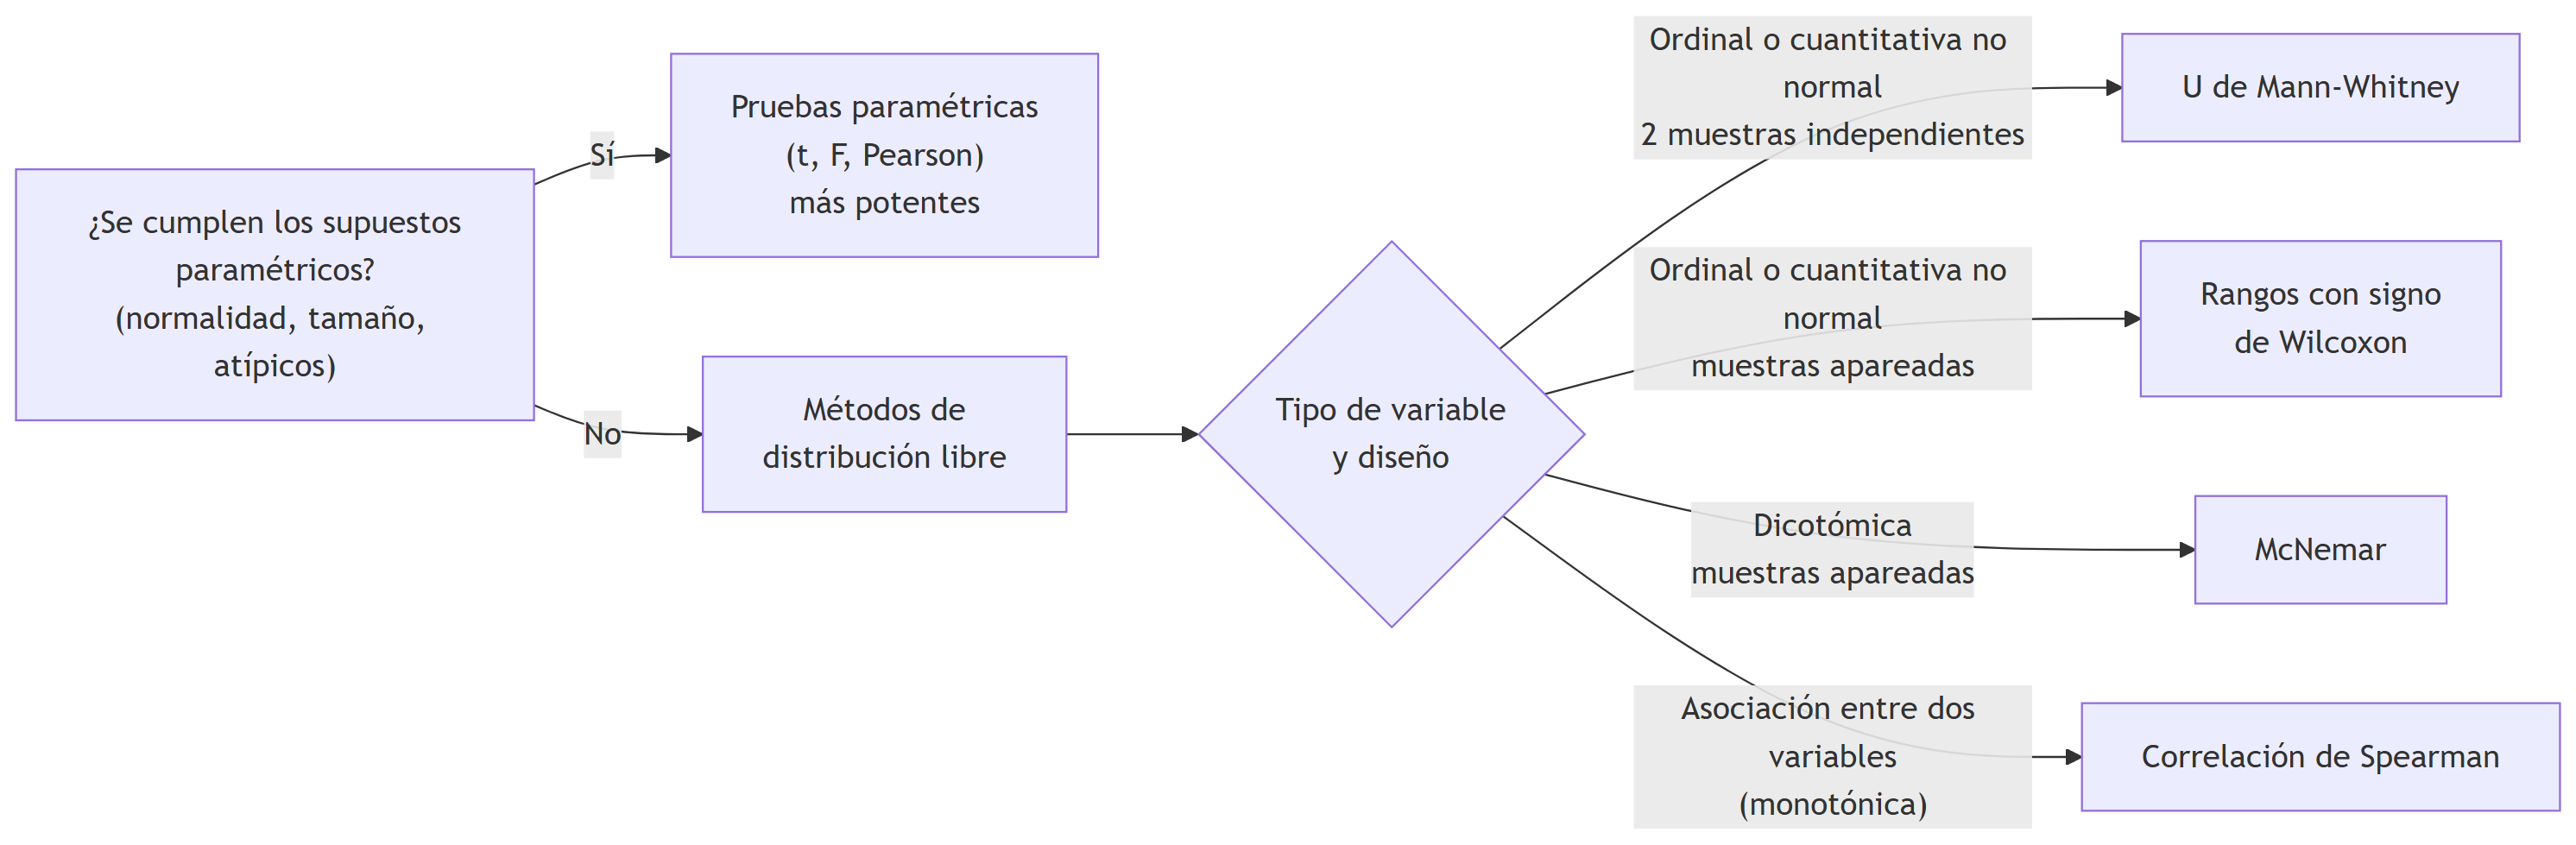
\includegraphics[width=13.47in,height=4.42in]{12_no_param_files/figure-latex/mermaid-figure-1.png}

Marco conceptual de la Unidad de Métodos No Paramétricos

\section{\texorpdfstring{\textbf{Actividad de
pre-clase}}{Actividad de pre-clase}}\label{actividad-de-pre-clase-6}

Deberá subir los siguientes archivos al cuaderno de \emph{notebooklm}, y
preguntarle cuál es la pregunta de investigación y los objetivos
propuestos en los trabajos.

Además, deberá pedirle a la IA, basándose en los ejercicios guiados de
la primera parte del script de R, que construya un flujo de trabajo
común que le permitan esquematizar sus análisis (la dinámica de la clase
será similar a la clase anterior).

\begin{itemize}
\tightlist
\item
  \href{./TRABAJOS\%20EPIST/np/009_pruebas_no_parametricas.R}{009\_pruebas\_no\_parametricas.R}
\item
  \href{./TRABAJOS\%20EPIST/np/GRUPO\%201_SEM2_2026.docx}{GRUPO
  1\_SEM2\_2026.docx}
\item
  \href{./TRABAJOS\%20EPIST/np/Grupo\%2010_\%20Seminario\%202_2026.docx}{Grupo
  10\_ Seminario 2\_2026.docx}
\item
  \href{./TRABAJOS\%20EPIST/np/GRUPO\%2011_SEMINARIO\%202_2026.docx}{GRUPO
  11\_SEMINARIO 2\_2026.docx}
\item
  \href{./TRABAJOS\%20EPIST/np/Grupo\%203_Sem\%202_2026.docx}{Grupo
  3\_Sem 2\_2026.docx}
\end{itemize}

\section{Micro-ejercicios de aplicación
(optativos)}\label{micro-ejercicios-de-aplicaciuxf3n-optativos-9}

Los siguientes micro-ejercicios te permitirán practicar los conceptos
revisados en esta unidad. Puedes copiar y pegar las preguntas en un
script de R local, o bien utilizar \texttt{webR}, que es la versión
\emph{online} de R, disponible en esta guía.

\texttt{Nota}: los ejercicios están inspirados en trabajos científicos
publicados, pero contienen datos simulados. Por lo tanto, los resultados
obtenidos deben interpretarse únicamente con fines didácticos y no como
evidencia científica.

La finalidad es familiarizarse con el análisis estadístico y con el uso
de R a partir de situaciones similares a las que pueden encontrarse en
investigaciones reales.

\begin{Shaded}
\begin{Highlighting}[]

\CommentTok{\# =============================================================================}
\CommentTok{\# EJERCICIO 1 {-} Germinación de poroto bajo estrés salino (U de Mann{-}Whitney)}
\CommentTok{\# =============================================================================}
\CommentTok{\# Pregunta estadística: ¿Difiere la mediana de semillas germinadas entre el}
\CommentTok{\# control (0 mM) y el tratamiento salino (100 mM NaCl)?}
\CommentTok{\#}
\CommentTok{\# Consignas:}
\CommentTok{\# 1. Identificar la variable respuesta (y) y la variable de grupo (x), indicando}
\CommentTok{\#    su tipo.}
\CommentTok{\# 2. Realizar un boxplot comparativo entre ambos grupos y calcular medianas e IQR.}
\CommentTok{\# 3. Plantear las hipótesis (H0 y H1) y el nivel de significancia.}
\CommentTok{\# 4. Aplicar la prueba U de Mann{-}Whitney y concluir con la decisión estadística.}

\NormalTok{germinadas\_control }\OtherTok{=} \FunctionTok{c}\NormalTok{(}\DecValTok{18}\NormalTok{, }\DecValTok{19}\NormalTok{, }\DecValTok{20}\NormalTok{, }\DecValTok{17}\NormalTok{, }\DecValTok{19}\NormalTok{, }\DecValTok{20}\NormalTok{, }\DecValTok{18}\NormalTok{, }\DecValTok{19}\NormalTok{)}
\NormalTok{germinadas\_sal     }\OtherTok{=} \FunctionTok{c}\NormalTok{(}\DecValTok{12}\NormalTok{, }\DecValTok{10}\NormalTok{, }\DecValTok{14}\NormalTok{, }\DecValTok{11}\NormalTok{, }\DecValTok{9}\NormalTok{, }\DecValTok{13}\NormalTok{, }\DecValTok{10}\NormalTok{, }\DecValTok{12}\NormalTok{)}


\CommentTok{\# =============================================================================}
\CommentTok{\# EJERCICIO 2 {-} Calidad de agua en ambientes periglaciares (Wilcoxon apareado)}
\CommentTok{\# =============================================================================}
\CommentTok{\# Pregunta estadística: ¿Difiere la mediana del índice biótico antes y después}
\CommentTok{\# del inicio de la exploración minera en las mismas estaciones?}
\CommentTok{\#}
\CommentTok{\# Consignas:}
\CommentTok{\# 1. Indicar por qué las observaciones son apareadas y qué tipo de variable es}
\CommentTok{\#    el índice biótico.}
\CommentTok{\# 2. Graficar las diferencias (antes {-} después) por estación y calcular medianas.}
\CommentTok{\# 3. Plantear las hipótesis y el nivel de significancia.}
\CommentTok{\# 4. Aplicar la prueba de rangos con signo de Wilcoxon y concluir.}

\NormalTok{indice\_antes   }\OtherTok{=} \FunctionTok{c}\NormalTok{(}\DecValTok{8}\NormalTok{, }\DecValTok{9}\NormalTok{, }\DecValTok{7}\NormalTok{, }\DecValTok{8}\NormalTok{, }\DecValTok{9}\NormalTok{, }\DecValTok{8}\NormalTok{, }\DecValTok{10}\NormalTok{, }\DecValTok{7}\NormalTok{, }\DecValTok{8}\NormalTok{)}
\NormalTok{indice\_despues }\OtherTok{=} \FunctionTok{c}\NormalTok{(}\DecValTok{5}\NormalTok{, }\DecValTok{6}\NormalTok{, }\DecValTok{4}\NormalTok{, }\DecValTok{6}\NormalTok{, }\DecValTok{5}\NormalTok{, }\DecValTok{7}\NormalTok{, }\DecValTok{6}\NormalTok{, }\DecValTok{5}\NormalTok{, }\DecValTok{4}\NormalTok{)}


\CommentTok{\# =============================================================================}
\CommentTok{\# EJERCICIO 3 {-} Desinfección de patógenos en frutos de naranjo (McNemar)}
\CommentTok{\# =============================================================================}
\CommentTok{\# Pregunta estadística: ¿Cambia la proporción de superficies con patógenos}
\CommentTok{\# presentes antes y después del tratamiento térmico?}
\CommentTok{\#}
\CommentTok{\# Consignas:}
\CommentTok{\# 1. Armar la tabla 2x2 de datos apareados (antes/después) y justificar por qué}
\CommentTok{\#    corresponde McNemar y no Chi{-}cuadrado de independencia.}
\CommentTok{\# 2. Plantear las hipótesis y el nivel de significancia.}
\CommentTok{\# 3. Aplicar la prueba de McNemar (sin y con corrección de continuidad).}
\CommentTok{\# 4. Interpretar el resultado en función de los pares discordantes.}

\NormalTok{tabla\_patogenos }\OtherTok{=} \FunctionTok{matrix}\NormalTok{(}\FunctionTok{c}\NormalTok{(}\DecValTok{3}\NormalTok{, }\DecValTok{16}\NormalTok{, }\DecValTok{1}\NormalTok{, }\DecValTok{5}\NormalTok{), }\AttributeTok{nrow =} \DecValTok{2}\NormalTok{, }\AttributeTok{byrow =} \ConstantTok{TRUE}\NormalTok{,}
                         \AttributeTok{dimnames =} \FunctionTok{list}\NormalTok{(}\AttributeTok{Antes =} \FunctionTok{c}\NormalTok{(}\StringTok{"Presente"}\NormalTok{, }\StringTok{"Ausente"}\NormalTok{),}
                                         \AttributeTok{Despues =} \FunctionTok{c}\NormalTok{(}\StringTok{"Presente"}\NormalTok{, }\StringTok{"Ausente"}\NormalTok{)))}


\CommentTok{\# =============================================================================}
\CommentTok{\# EJERCICIO 4 {-} Altitud y tolerancia al frío en ecotipos de quinua (Spearman)}
\CommentTok{\# =============================================================================}
\CommentTok{\# Pregunta estadística: ¿Existe asociación monotónica positiva entre la altitud}
\CommentTok{\# del sitio de origen y la tolerancia a la germinación en frío?}
\CommentTok{\#}
\CommentTok{\# Consignas:}
\CommentTok{\# 1. Identificar la variable independiente y la dependiente, indicando su tipo.}
\CommentTok{\# 2. Realizar el diagrama de dispersión entre ambas variables.}
\CommentTok{\# 3. Plantear las hipótesis y el nivel de significancia.}
\CommentTok{\# 4. Aplicar la correlación de Spearman e interpretar el coeficiente y la}
\CommentTok{\#    decisión estadística.}

\NormalTok{altitud         }\OtherTok{=} \FunctionTok{c}\NormalTok{(}\DecValTok{2200}\NormalTok{, }\DecValTok{2500}\NormalTok{, }\DecValTok{2800}\NormalTok{, }\DecValTok{3100}\NormalTok{, }\DecValTok{3400}\NormalTok{, }\DecValTok{3700}\NormalTok{, }\DecValTok{4000}\NormalTok{, }\DecValTok{4200}\NormalTok{)}
\NormalTok{tolerancia\_frio }\OtherTok{=} \FunctionTok{c}\NormalTok{(}\DecValTok{2}\NormalTok{, }\DecValTok{3}\NormalTok{, }\DecValTok{4}\NormalTok{, }\DecValTok{6}\NormalTok{, }\DecValTok{7}\NormalTok{, }\DecValTok{8}\NormalTok{, }\DecValTok{9}\NormalTok{, }\DecValTok{10}\NormalTok{)}


\CommentTok{\# =============================================================================}
\CommentTok{\# EJERCICIO 5 {-} Macroinvertebrados en arroyos puneños (U de Mann{-}Whitney)}
\CommentTok{\# =============================================================================}
\CommentTok{\# Pregunta estadística: ¿Es mayor la mediana de riqueza taxonómica en tramos}
\CommentTok{\# sin pastoreo que en tramos con pastoreo de camélidos?}
\CommentTok{\#}
\CommentTok{\# Consignas:}
\CommentTok{\# 1. Formular la pregunta de investigación e identificar las variables (y, x).}
\CommentTok{\# 2. Realizar el boxplot comparativo y calcular medianas e IQR.}
\CommentTok{\# 3. Plantear las hipótesis y el nivel de significancia.}
\CommentTok{\# 4. Aplicar la prueba U de Mann{-}Whitney y concluir sobre el efecto del pastoreo.}

\NormalTok{con\_pastoreo }\OtherTok{=} \FunctionTok{c}\NormalTok{(}\DecValTok{4}\NormalTok{, }\DecValTok{5}\NormalTok{, }\DecValTok{3}\NormalTok{, }\DecValTok{6}\NormalTok{, }\DecValTok{4}\NormalTok{, }\DecValTok{3}\NormalTok{, }\DecValTok{5}\NormalTok{, }\DecValTok{4}\NormalTok{)}
\NormalTok{sin\_pastoreo }\OtherTok{=} \FunctionTok{c}\NormalTok{(}\DecValTok{9}\NormalTok{, }\DecValTok{11}\NormalTok{, }\DecValTok{8}\NormalTok{, }\DecValTok{12}\NormalTok{, }\DecValTok{10}\NormalTok{, }\DecValTok{9}\NormalTok{, }\DecValTok{11}\NormalTok{, }\DecValTok{10}\NormalTok{)}
\end{Highlighting}
\end{Shaded}

\bookmarksetup{startatroot}

\chapter*{R en la web y Geogebra}\label{r-en-la-web-y-geogebra}
\addcontentsline{toc}{chapter}{R en la web y Geogebra}

\markboth{R en la web y Geogebra}{R en la web y Geogebra}

\section*{R en la web}\label{r-en-la-web}
\addcontentsline{toc}{section}{R en la web}

\markright{R en la web}

En este entorno podrás ejecutar algunas funciones de R.

\begin{Shaded}
\begin{Highlighting}[]

\NormalTok{\# Códigos acá}


\end{Highlighting}
\end{Shaded}

\begin{center}\rule{0.5\linewidth}{0.5pt}\end{center}

\section*{Paquete resumiR}\label{paquete-resumir}
\addcontentsline{toc}{section}{Paquete resumiR}

\markright{Paquete resumiR}

La cátedra de Bioestadística y Diseño Experimental de la UNJu ha
desarrollado el paquete estadístico
\href{https://r-packages.io/packages/resumiR}{\{resumiR\}}, con
funciones que permiten obtener rápidamente una serie de medidas de
resumen y gráficos para datos numéricos discretos o continuos en series
simples. También permite obtener tablas de frecuencia clásicas y
gráficos cuando se desea realizar un análisis de series agrupadas. Su
objetivo es de aplicación didáctica para la clase instroductoria de
Bioestadística utilizando el software R, para las carreras de grado las
carreras de grado y otras ofertas educativas de la Facultad de Ciencias
Agrarias de la UNJu.

\begin{center}\rule{0.5\linewidth}{0.5pt}\end{center}

\section*{GeoGebra (Visualización
interactiva)}\label{geogebra-visualizaciuxf3n-interactiva}
\addcontentsline{toc}{section}{GeoGebra (Visualización interactiva)}

\markright{GeoGebra (Visualización interactiva)}

Como complemento al uso de software estadístico especializado, se
recomienda el empleo del módulo de \textbf{Distribuciones Estadísticas
de GeoGebra}. Esta herramienta permite al estudiante seleccionar una
distribución y especificar sus parámetros para obtener de forma
inmediata la representación gráfica de la función de densidad (en
variables continuas) o de la función de probabilidad (en variables
discretas).

El valor didáctico de GeoGebra yace en su capacidad para calcular la
probabilidad en un intervalo de forma visual, lo cual coincide con el
área bajo la función de densidad o la suma de probabilidades discretas.

~

~

Integrar esta práctica ofrece las siguientes \textbf{ventajas
estratégicas}:

\begin{itemize}
\tightlist
\item
  Andamiaje visual: Antes de realizar un cálculo con un programa
  estadístico, GeoGebra permite construir un modelo mental de la
  distribución. Esto ayuda a internalizar cómo los cambios en parámetros
  alteran la forma y posición de la curva.
\item
  Validación de resultados: Funciona como un mecanismo de control para
  verificar si los valores de probabilidad obtenidos mediante software
  son consistentes con la representación geométrica.
\item
  Transición del razonamiento al pensamiento: Al facilitar la
  manipulación interactiva de los límites de un intervalo, cada
  estudiante puede explorar escenarios del tipo \emph{``¿qué pasaría
  si\ldots?''}, fortaleciendo su capacidad de pensamiento estadístico al
  conectar la teoría abstracta con una representación espacial concreta.
\end{itemize}

La utilización del simulador de GeoGebra es muy intuitiva y de fácil
apropiación por parte de los estudiantes. No obstante, durante los
encuentros presenciales se realizarán instancias de acompañamiento y
demostraciones guiadas orientadas a explicitar su funcionamiento y
vincular las acciones realizadas en el entorno interactivo con los
conceptos estadísticos subyacentes.

\bookmarksetup{startatroot}

\chapter*{Referencias}\label{referencias}
\addcontentsline{toc}{chapter}{Referencias}

\markboth{Referencias}{Referencias}

\begin{itemize}
\item
  \textbf{Apuntes de Bioestadística. Con ejercicios resueltos.} Guía
  práctica de cátedra.
\item
  Lepš, J., \& Šmilauer, P. (2020). Biostatistics with R: An
  introductory guide for field biologists. Cambridge University Press.
\item
  Balzarini, M., Di Rienzo, J., Tablada, M., Gonzalez, L., Bruno, C.,
  Córdoba, M., Robledo, W., \& Casanoves, F. (s.f.). Bioestadística:
  Primera edición. {[}Editorial desconocida{]}.
\item
  Weaver, K. F., Morales, V. C., Dunn, S. L., Godde, K., \& Weaver, P.
  F. (2018). An introduction to statistical analysis in research: With
  applications in the biological and life sciences. John Wiley \& Sons.
\item
  Irizarry, R. A., \& Love, M. I. (2021, March 17). Data analysis for
  the life sciences (Version 2021-03-17). Leanpub.
\item
  Curry, E. (2020). Introduction to bioinformatics with R: A practical
  guide for biologists. CRC Press, Taylor \& Francis Group.
\end{itemize}




\end{document}
